\documentclass[oneside,12pt,openany]{book}

\usepackage[utf8x]{inputenc}
\usepackage[T1]{fontenc}
\usepackage{graphicx}
\usepackage{aas_macros}
\usepackage[space]{grffile}
\usepackage{latexsym}
\usepackage{IEEEtrantools}
\usepackage{longtable}
\usepackage{multirow,booktabs}
\usepackage{amsfonts,amsmath,amssymb}
\usepackage[numbers]{natbib}
\usepackage{tabularx}
% \usepackage[backend=bibtex,style=numeric,natbib=true]{biblatex}
% \usepackage[style=numeric,natbib=true]{biblatex}

% \usepackage[natbib, style=apa]{biblatex}
% \usepackage[backend=biber,style=ieee, maxnames=10]{biblatex}
% \usepackage[backend=bibtex,style=authoryear,natbib=true]{biblatex} 
\setcitestyle{square}
\usepackage{url}
\usepackage{hyperref}
% \usepackage[colorlinks,citecolor=blue]{hyperref}
\usepackage{longtable}
\usepackage[onehalfspacing]{setspace}
\hypersetup{colorlinks=true,pdfborder={0 0 0},linkcolor=blue,citecolor=blue }
% \usepackage{fullpage}
% \usepackage{caption}
% \renewcommand{\textfraction}{0.05} 
%%
\usepackage[autostyle=true]{csquotes}
% \usepackage{titlesec}
\usepackage{placeins}
\usepackage{subcaption}
\graphicspath{{Figures/}} % Specifies the directory where pictures are stored
\usepackage[labelfont=bf]{caption}
\usepackage{listings}
\usepackage{float}
\usepackage{enumitem}
\usepackage[toc,page]{appendix}
\newcommand\theo[1]{\textcolor{magenta}{#1}}
% \usepackage{bm}
% \usepackage{flafter}
% \usepackage[left=5cm,top=2.0cm,bottom=1.5cm,right=2cm,bindingoffset=.5cm]{geometry}
% \usepackage[top=2cm, bottom=2cm, outer=1cm, inner=2.1cm, headsep=14pt]{geometry}
\usepackage[paper=a4paper,top=2.5cm, bottom=2cm, outer=3.8cm, inner=2.5cm, bindingoffset=.5cm]{geometry}
% \geometry{
% 	paper=a4paper, % Change to letterpaper for US letter
% 	inner=2.5cm, % Inner margin
% 	outer=3.8cm, % Outer margin
% 	bindingoffset=.5cm, % Binding offset
% 	top=1.5cm, % Top margin
% 	bottom=1.5cm, % Bottom margin
% 	%showframe, % Uncomment to show how the type block is set on the page
% }
% \usepackage{fancyhdr} 
% \fancyhf{}
% \cfoot{\thepage}
% \pagestyle{fancy}

\usepackage{fancyhdr}
\renewcommand{\chaptermark}[1]{\markboth{#1}{}}
\renewcommand{\sectionmark}[1]{\markright{#1}}
\pagestyle{fancy}
\fancyhf{}
\fancyhead[LE,RO]{\thepage}
\fancyhead[LO]{\itshape\nouppercase{\rightmark}}
\fancyhead[RE]{\itshape\nouppercase{\leftmark}}
% \fancyhead[LO]{\nouppercase{\rightmark}}
% \fancyhead[RE]{\nouppercase{\leftmark}}
\renewcommand{\headrulewidth}{1pt}

\setcounter{secnumdepth}{4}
\setcounter{tocdepth}{4}
% \DeclareMathOperator{\sinc}{sinc}
% \DeclarePairedDelimiter\ceil{\lceil}{\rceil}
% \DeclarePairedDelimiter\floor{\lfloor}{\rfloor}
% \usepackage[colorlinks=false,linkcolor=blue]{hyperref}%
%%
\captionsetup[table]{skip=10pt}
\newcommand{\bm}{\boldsymbol}
% \newcommand\numberthis{\addtocounter{equation}{1}\tag{\theequation}}
% \newcommand{\etal}{\textit{et al.}}
% \def\nl{\\\hline}

\let\cleardoublepage\clearpage
\DeclareMathOperator{\sinc}{sinc}
\begin{document}

\frontmatter
\begin{titlepage}

\newcommand{\HRule}{\rule{\linewidth}{0.5mm}} % Defines a new command for the horizontal lines, change thickness here

\center % Center everything on the page
 
%----------------------------------------------------------------------------------------
%	LOGO SECTION
%----------------------------------------------------------------------------------------


\includegraphics[width=0.4\columnwidth]{Images/Rhode}\\[1cm] % Include a department/university logo - this will require the graphicx package

%----------------------------------------------------------------------------------------

%----------------------------------------------------------------------------------------
%	TITLE SECTION
%----------------------------------------------------------------------------------------

\HRule \\[0.4cm]
{ \huge Exploring Intensity Mapping Techniques Via Simulations}\\[0.4cm]
% { \huge {\sc meqsilhouette}: Exploring Intensity Mapping Techniques Via Simulations}\\[0.4cm]
\HRule \\[1.5cm]


\begin{center}
 {\large A thesis submitted in fulfilment of the requirements for the degree of \textbf{Doctor of Philosophy}} \\
%  {\large \textbf{MASTER OF SCIENCE}} \\
 {\large in the Department of Physics and Electronics,} \\
 {\large Rhodes University}
\end{center}
\vspace{0.02\textheight}

%----------------------------------------------------------------------------------------
%	AUTHOR SECTIONSpace & Atmospheric Research Group
%----------------------------------------------------------------------------------------

\begin{minipage}{0.45\textwidth}
\begin{flushleft}\large 
\emph{Author:} \\
Theophilus  {\sc Ansah-Narh}\\
\end{flushleft}
\end{minipage}
\begin{minipage}{0.45\textwidth}

\begin{flushright} \large
\emph{Supervisors:} \\
Prof. Oleg M. {\sc Smirnov} \\
Prof. Filipe B. {\sc Abdalla} \\
Dr. Khan M. B. {\sc Asad} \\
\end{flushright}
\end{minipage}\\[2cm]

\vfill
{\large February 02, 2019}\\[4cm]
% \vfill

% {\large \today}\\[4cm]

\end{titlepage}
%%



%**** DECLARATION **************
% ******************************
\chapter*{Statement of Originality}
\vspace*{-2em}
%  I acknowledge that plagiarism is wrong and hereby declare that the work contained in this document and in the supporting software is my own, save for that which is properly acknowledged. 
% I recognise that much of the work in this thesis has already been presented in our recent paper \citep{Blecher_2016}.
% This thesis is essentially an expanded version of the paper and as the latter was published first, some of the material from it has been reproduced directly. 
% For paragraphs reproduced directly, we indent the text, place it in quotations and cite \citep{Blecher_2016} after the quotation. In addition, notes have been made at the beginning of certain sections or in the captions of figures to denote reproduction of material from our paper.

 I, {\sc Ansah-Narh} Theophilus, assert that the ideas contained in this thesis are my own, and so the thesis has not been formerly put forward for a qualification at any 
 other tertiary institution. 
 \\~\\
%  \vspace*{2em}
 \noindent Signed:\\
\rule[0.5em]{25em}{0.5pt} % This prints a line for the signature
 
\noindent Date:\\
\rule[0.5em]{25em}{0.5pt} % This prints a line to write the date
\addcontentsline{toc}{chapter}{Statement of Originality}
%%
%****** PUBLICATION **************
% ******************************
\chapter*{Publications}
\vspace*{-2em}
%%
This research is largely drawn from the following publications:

\begin{itemize}
 \item T. Ansah-Narh, F. B. Abdalla, O. M. Smirnov, K. M. B. Asad and J. R. Shaw, (2018). Simulations of Systematic Direction-dependent Instrumental Effects
in Intensity Mapping Experiments. \emph{Monthly Notices of the Royal Astronomical Society}, 481 (2), 2694--2710.

\item K. M. B. Asad, J. N. Girard, M. de Villiers, T. Ansah-Narh, K. Iheanetu, O. Smirnov, M. G. Santos, R. Lehmensiek,
K. Thorat, S. Makhathini and others, Primary Beam Effects of Radio Astronomy Antennas – II. Modelling the MeerKAT L-band beam using
holography. \emph{Monthly Notices of the Royal Astronomical Society}, accepted.
\end{itemize}

\noindent I hereby confirm that some of the text and figures from these have been reproduced directly. In addition, where I have mentioned the work published by others, credit has been given to this effect. 
%%
\addcontentsline{toc}{chapter}{Publications}
\chapter*{Abstract} 
%2 paragraphs : 1 intro, 2. Results
%Intro
%eht
 \vspace*{-2em}
% 

The study used intensity mapping technique to observe the combined radio emissions of CO and HI emanating from a diffuse source. Antenna elements with short separations like
KAT-7 (not in operation now) and SKA1-mid can be used for such observation. Despite the potential of this technique, it is subject to exact foreground reduction of continuum signal
from the Milky Way galaxy and other radio sources beyond. In addition, the signal is dominated by direction-dependent effects and the primary beam being the most serious effect,
since it controls the full intensity of the measured signal. Furthermore, the inaccuracies in the receivers, cause part of the foreground to seep into the absolute intensity, making
it difficult to observe the CO or HI signal. For the current on-going SKA instruments and future aperture arrays, these will be affected by antenna pointing errors and polarization
leakages. To address these problems, first, we create a dense set of dipole positions with a complete secondary blockage to mimic the illumination pattern of KAT-7-like dish. Second,
we use Zernike model to reconstruct MeerKAT L-band beams and then third, we try to simulate EM beams of SKA1-mid as an optical telescope. Next we perturb these beams by introducing
realistic errors in them. We then simulate these beams (true and corrupted) with the foreground to estimate for the CO and HI signal. At the end, our simulation shows that,
if we consider a correct model of the primary beam, then the intrinsic partial leakage of linear polarization ($|Q + iU|_{T} \longrightarrow I$) is given at $\approx 1.0 \%$. 
Furthermore, when we correct for the beam errors in Stokes $I$ then, it is possible to evaluate the angular spectrum of both CO and HI  at a multipole moment of $l \lesssim 50$, 
however, this is vice versa if we do calibrate for the beam erros. Finally, the study shows that, Zernike and convolution techniques are good models for intensity mapping experiments. 
%%
\addcontentsline{toc}{chapter}{Abstract}

\chapter*{Acknowledgements}
%  \vspace*{-0.2\textheight}
% \hspace*{-0.6in}
%  \raggedbottom
 \vspace*{-2em}
 The completion of this research is made up of immense inputs from many people to whom I owe a debt of gratitude. 
First and foremost, I thank my supervisors: Prof. Oleg M. Smirnov who doubles as the 
SKA Chair in Radio Astronomy Techniques and Technologies (RATT), which is hosted by Rhodes University 
and my main supervisor, particularly, for the strong affection he puts in everything he does and for his enormous understanding 
in Computational Mathematics and Radio Interferometry, Prof. Filipe B. Abdalla, for his expertise in Cosmology and Intensity Mapping Experiments and for the
patience he had in supporting me especially during the first year of the research. Also, Dr. Khan M. B. Asad for his understanding in Intensity Mapping Experiments.
I also show my appreciation to everyone who directly took part in the realisation of this work, particularly 
to Dr. Richard Shaw for helping me out with the foreground simulations and Dr. Jamie Leech for teaching me how to use the {\tt GRASP} software.
% I acknowledge many individuals, who even if in a less technical way, have been and are of vital importance for me throughout this research experience.
My course mates deserve the best recognition. Sphe, Marcel, Ridhima, Liju, Kela, Alex and the others 
have been wonderful companions throughout the study period. I would like to thank my family, Mr. Francis D. Narh (father),
Mrs. Salome Nortey (mother), Samuel Annor Narh (brother), Esther Amatsu Narh, Christiana Koryoonmaatso Narh (sisters), Patricia Opoku (wife), Adelaide and Salome (daughters) 
for their love and trust. Lastly, I am very grateful to the SKA and NRF for supporting this research.
% Without them this accomplishment would have been unachievable.
 \addcontentsline{toc}{chapter}{Acknowledgements}
% 
% This thesis is the culmination of the efforts of many individuals to whom I owe my most sincere appreciation. 
% First of all I would like to thank my supervisors: Prof. Oleg M. Smirnov who doubles as the 
% SKA Chair in Radio Astronomy Techniques and Technologies (RATT), which is hosted by Rhodes University 
% and my main supervisor, especially for the passion he brings to everything he does and for his great knowledge
% in Mathematics and Radio Interferometry, Dr. Filipe B. Abdalla, for his expertise in Cosmology and Intensity Mapping Experiments and for the
% patience he had in supporting me especially during the first year of the research. Also, Dr. Khan M. B. Asad for his understanding in Intensity Mapping Experiments.
% I would like to thank everybody who was directly involved in the realisation of this project, particularly 
% to Dr. Richard Shaw for helping me out with the foreground simulations and Dr. Jamie Leech for teaching me how to use the GRASP software.
% I acknowledge many individuals, who even if in a less technical way, have been and are of vital importance for me throughout this research experience.
% My course mates deserve the best recognition. Sphe, Marcel, Ridhima, Liju, Kela, Alex and the others 
% have been wonderful companions throughout the study period. I would like to thank my family, Mr. Francis D. Narh (father),
% Mrs. Salome Nortey (mother), Samuel Annor Narh (brother), Esther Amatsu Narh, Christiana Koryoonmaatso Narh (sisters), Patricia Opoku (wife) 
% and Adelaide Tsako Doku (daughter) for their love and trust. Lastly, I am very grateful to the SKA and NRF for supporting this research.
% Without them this accomplishment would have been unachievable.

% \chapter*{Plagiarism declaration}
%  \addcontentsline{toc}{chapter}{Plagiarism}
%  I acknowledge that plagiarism is wrong and hereby declare that the work contained in this document and in the supporting software is my own, save for that which is properly acknowledged. I recognise that much of the work in this thesis has already been presented in our recent paper \citep{Blecher_2016}. This thesis is essentially an expanded version of the paper and as the latter was published first, some of the material from it has been reproduced directly. For paragraphs reproduced directly, we indent the text, place it in quotations and cite \citep{Blecher_2016} after the quotation. In addition, notes have been made at the beginning of certain sections or in the captions of figures to denote reproduction of material from our paper.
%  \vspace{55pt}
 
% Tariq Dylan Blecher
%  \clearpage
%   \topskip0pt
%   \vspace*{\fill}
%     \begin{center}
%      \huge
% %      The {\sc meqsilhouette} source code is at present still proprietary of SKA SA as in hence unavailable to the public at the time of writing. However, we do include an appendix which details installation and usage as reference for private or future public use.
%     \end{center}
  \vspace*{\fill}
\tableofcontents
\phantomsection
\listoffigures
\addcontentsline{toc}{chapter}{\listfigurename}
\listoftables
\addcontentsline{toc}{chapter}{\listtablename}

\mainmatter % Begin numeric (1,2,3...) page numbering
% \pagestyle{fancy} % Return the page headers back to the "thesis" style
% Chapter 1

\chapter{Introduction}\label{Chapter1} % Main chapter title

 % For referencing the chapter elsewhere, use \ref{Chapter1} 

%----------------------------------------------------------------------------------------

% Define some commands to keep the formatting separated from the content 
\newcommand{\keyword}[1]{\textbf{#1}}
\newcommand{\tabhead}[1]{\textbf{#1}}
\newcommand{\code}[1]{\texttt{#1}}
\newcommand{\file}[1]{\texttt{\bfseries#1}}
\newcommand{\option}[1]{\texttt{\itshape#1}}

%\lhead{Chapter 1. \emph{Introduction}} 
%----------------------------------------------------------------------------------------
\textbf{Overview}\\
% \HRule \\[0.5cm]
\par\noindent\rule{\textwidth}{0.4pt}\\
\textit{This chapter introduces us to the general background of the research by briefly discussing the origin of the 21 cm radio line
and then moves on to discuss the significance of intensity mapping experiments. The research problems, key objectives, justification and the entire structure of the thesis 
are also outlined.}
\par\noindent\rule{\textwidth}{0.4pt}\\
% \HRule \\[1.5cm]
%
%  \enquote{spin-flip}
%----------------------------------------------------------------------------------------
\section{The 21 cm Radio Emission Line}	   \label{chap1:21cm}		
%%
% \vspace*{-2em}
Despite the fact that space is very empty and there is a great distance between the stars in the Milky Way, the gap between these
stars consists of dust and a very diffuse medium of gas. Astronomers refer to this matter and the radiation in space  as the \emph{interstellar medium} (ISM\footnote{\url{http://www-ssg.sr.unh.edu/ism/what1.html}}). The  interstellar gas can be found in molecular (mainly $\mathrm{H_{2}}$), ionic ($\mathrm{HII}$) or atomic (HI) form and 
it is composed of Hydrogen ($\approx 70\,\%$) followed by Helium ($\approx 28\,\%$) and the rest being heavy elements (Oxygen, Carbon and Nitrogen). 
The molecular and atomic Hydrogen gases are located in the colder dense regions of the ISM at ($T \sim {10-30}$)K and ($T \sim 50-100$)K respectively whilst, the ionic gas is in the warmer ($T \sim  {10^{3} - 10^{4}}$)K more dilute regions \citep{knee2001massive}.

% The simplest atom to understand among all the other kinds is the neutral hydrogen. It consists of a single proton and an electron with positive and negative charges respectively.
% These charges are attracted to each other by pulling the protons and the electrons together. 
% If the electron loses energy, then it moves closer to the proton, but if the electron gains energy, it is the vice versa. 
% Therefore, the energy released when an electron drops from a higher level to a lower level as shown in Fig.~\ref{fig:Hspin} (right  plot) 
% is known as the electromagnetic (EM) radiation. Depending on how far the electron has fallen, this can be a radio wave, visible light or even an
% ultra-violet. 
% %%

% Considering the neutral hydrogen (HI) atom in the Universe,
Nevertheless, a large portion of the hydrogen gas (mostly in atomic form) in the ISM is in the least energy state \citep{klessen2016physical}. 
Usually, both the proton and electron of a Hydrogen atom spin in the same state but, it happens very occasionally that (in every $11$ million years), 
the proton and the electron within the hydrogen atom 
will realign themselves slightly (that is, change the direction of the spin spontaneously) as shown in Fig.~\ref{fig:Hspin}, 
making the electrons to flip a little bit closer to the proton in a very specific way.
The fact that this is specific means that the frequency at which the EM radiation is given out is always the same, 
that is, the frequency is approximately $1420.406 \, \rm{MHz}$, and therefore, using large radio telescopes, radio
astronomers can observe the $21$ cm line (at  $1420.406$ MHz) even in very distant galaxies.
This 21 cm radio emission line was first proposed in the early 1940s by van de Hulst and is very famous in radio astronomy because 
it is the most powerful way of observing HI and making maps from it. 
Most often, when we observe the emission line, the distribution of this line  is Doppler shifted. This is because, a spiral galaxy rotates
in such a way that, if it is marginally edge-on to our line of sight, a portion of the HI regions
move away from us whilst others move towards us. This Doppler effect broadens the 21 cm
line into a double peak. It redshifts the radiation from the regions that move away from us
and blueshifts the vice versa.Therefore, the faster the rotation of the galaxy, the greater the
line broadening. It redshifts the radiation from the regions that move away from us
and blueshifts the vice versa.Therefore, the faster the rotation of the galaxy, the greater the
line broadening. Many academic works \citep{condon2016essential,wilson2013tools,wilson2009tools} give an in-depth explanation of this section.
% The unique wavelength this radiation has means we can actually detect the motion of the hydrogen compound to our motion. 
% This phenomenon is due to the Doppler effect. When a radio source is moving and giving out a signal or some
% kind of radiation, the fact that it is moving affects the frequency or the wavelength of that radiation. For instance, 
% relating this to our daily activities, when a siren or a car engine goes pass you, you will hear a change in the peak or tone. 
% Let assume a hydrogen atom is moving towards us and giving out radiation, then this radiation will be blueshifted with a shorter wavelength. 
% On the other hand, if the atom is moving away from us, it will be redshifted with a longer wavelength. This is really a useful extra piece of 
% information these observations give us. Using the redshift information, we will be able to determine distant galaxies in the universe. 

%%
\begin{figure}[ht]
	  \centering	     
	  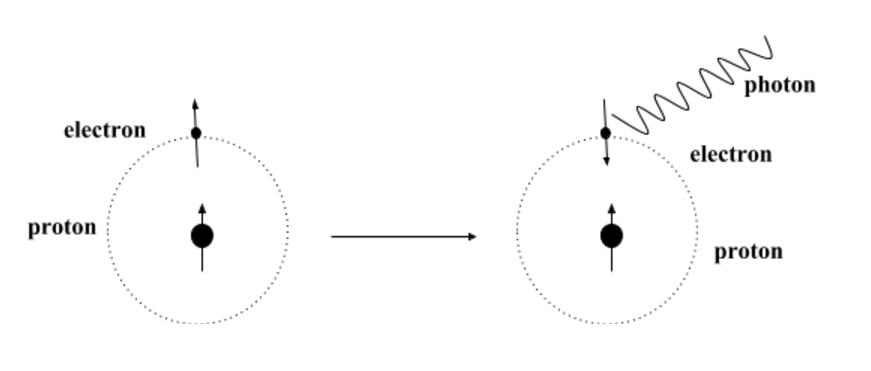
\includegraphics[width=3.8in]{c1/Hspin}	   
	  \caption{When the electron of a neutral hydrogen atom flips its spin, energy is released at a wavelength of $21\, \rm{cm}$. This figure is obtained from \cite[pg. 113]{ferrara2008first}.}
	  \label{fig:Hspin}
      \end{figure}
      \FloatBarrier
%%
The next section discusses how intensity mapping (IM) experiment is used to measure the distribution of the sky.

% %%
%----------------------------------------------------------------------------------------
% %

\section{HI Intensity Mapping} \label{chap1:h1mapping}
%%
The motivation to study cosmology in this present-day is to understand the massive size of the Universe, understand how the Universe expands and the distribution of everything. 
In order to do this, an observational time  is needed to really map out the large volume of data. Over the past two decades, the galaxy redshift surveys 
such as 2dF\footnote{\url{http://www.2dfgrs.net/}}, 6dF\footnote{\url{http://www-wfau.roe.ac.uk/6dFGS/}}, WiggleZ\footnote{\url{http://wigglez.swin.edu.au/site/}}, 
BOSS\footnote{\url{http://www.sdss3.org/surveys/boss.php}}, and SDSS\footnote{\url{http://www.sdss.org/}} 
use the optical spectroscopy to specifically observe millions of individual galaxies, determine each redshift and use these to estimate the energy distribution for each \citep{2009astro2010S.234P,1996ApJ...461...38S,1995ApJ...446..457S}. This approach really consumes a lot of time due to the map out of individual galaxies and also, it is very difficult to resolve faint sources. 
The total optical surveys used to localize the Universe in this way is approximately $1\%$ \citep{2009astro2010S.234P}.\\ %peterson200921}
%%
\indent Meanwhile, recent researches \citep{camera2014cosmology,2008PhRvL.100i1303C,2015aska.confE..19S,2015aska.confE..35W,2014MNRAS.441.3271W} on IM have shown that, this alternative approach does not resolve all the structures in the Universe but can actually provide us with a very good idea of how things are distributed as displayed in
Fig.~\ref{fig:implotb}. Here, the figure shows the variations in the simulated HI brightness temperature, where 
red indicates over-density and blue under-density, making it possible to infer from this map. From a cosmological point of view, that is sufficient enough because we can still see a lot of the features in Fig.~\ref{fig:implotb} map even though it's horribly pixelated as compared to Fig.~\ref{fig:implota}.
% %%
% 
\begin{figure}[H]
\begin{minipage}{\linewidth}
\centering
    \begin{subfigure}[b]{0.49\textwidth}
	      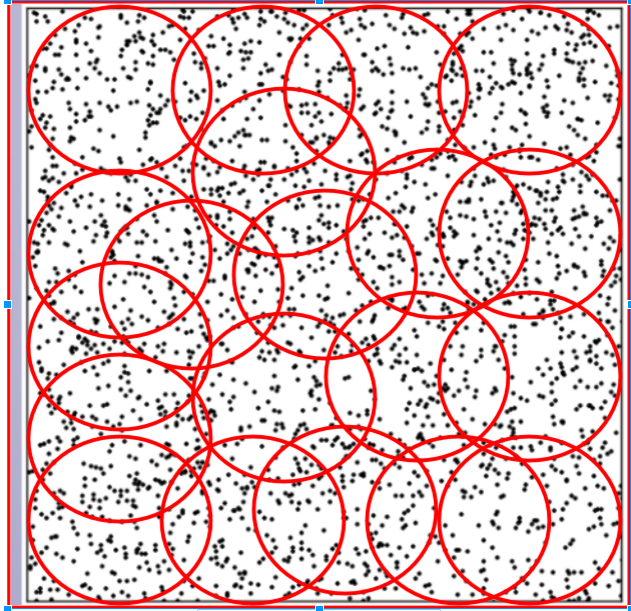
\includegraphics[width=\textwidth]{c1/g4}               
	      \caption{}                
	      \label{fig:implota}
      \end{subfigure}       
      \begin{subfigure}[b]{0.48\textwidth}
	      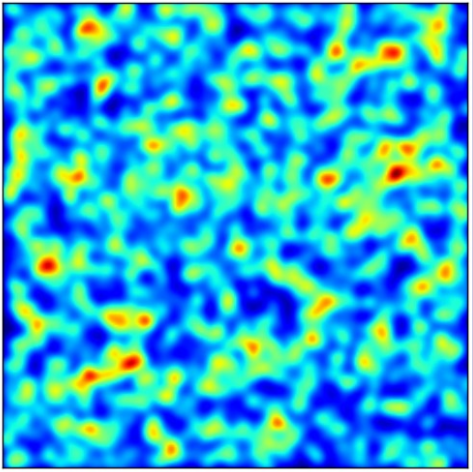
\includegraphics[width=\textwidth]{c1/g3}                
	      \caption{}               
	      \label{fig:implotb}
      \end{subfigure}        
	\end{minipage}
      \caption{Simulated variations in the 21 cm emission brightness temperature. The red rings in (a) show how to perform IM experiment by observing multiple patches in the sky with 
      the radio telescope in order to measure the 21 cm  emission to produce (b). Note that this figure is very similar to the one discussed in \citep{2009astro2010S.234P}.}%% \cite{peterson200921}
	\label{fig:implot}
\end{figure}
\FloatBarrier
% %

In terms of the observing strategy, a radio telescope (usually a big dish) is used to point and scan over the sky to measure the 21 cm spectral line. With this complementary approach, we can effectively map a large volume of the sky, since every frequency channel in the telescope will produce a different redshift of the HI. Note that, these big data obtained from the IM method can't really be achieved with any other method within the same period of time. These maps typically have a low spatial resolution, making it quite difficult to identify any single object as seen in Fig.~\ref{fig:implotb}. Nevertheless, the maps do have high redshift resolution due to the signal to noise in the instrument channels. Therefore, HI IM is the technique of integrating the spectral line flux over the whole HI mass function without selecting individual neutral objects.

Section~\ref{chap1:sec3} briefly discusses the importance of IM observational techniques and some of the current radio instruments purposely designed to perform this kind of experiment. 


% %%
% %----------------------------------------------------------------------------------------
% %%
% 
% %
\section{Significance of Intensity Mapping Techniques} \label{chap1:sec3}
%
The IM technique has the advantage of not resolving sources but instead measures diffuse sources that can be used to
generate tomographic maps of the Universe for many redshifts within the interval $0 < z < 6$ which is basically what the Square Kilometre Array (SKA) 
Phase I \citep{2010arXiv1008.2871G} is planning to do. In addition, the data produced from this technique contains spatial information that may be useful to 
measure Baryon Acoustic Oscillations (BAOs) \citep{2008PhRvL.100i1303C} which is one of the major incentive explored by the cosmologists and has led to the establishment of this method.
Measuring the BAOs for different redshifts would make us understand the expansion of the Universe. Furthermore, with the observational data from several lines, we
will also be able to cross-correlate the lines which can be used to remove the foreground from 21 cm observations. Finally,
the technique allows smaller and cheaper telescopes without long baselines such as HIRAX\footnote{{\url{https://www.acru.ukzn.ac.za/~hirax/}}}, to be used in such experiments,
hence increasing the science output in cosmology.\\
%%
\indent Presently, several IM experiments are in operation, such as the 
GBT\footnote{{\url{https://science.nrao.edu/facilities/gbt}}} (\enquote{Green Bank Telescope}), CHIME\footnote{{\url{https://chime-experiment.ca/}}} (\enquote{Canadian Hydrogen Intensity Mapping Experiment}),
Tianlai\footnote{{\url{http://tianlai.bao.ac.cn/}}} and FAST\footnote{{\url{http://fast.bao.ac.cn/en/}}} (\enquote{Five hundred metre Aperture Spherical Telescope}).
Among these instruments for IM experiments, the GBT produced the first HI signal at $z \sim 0.8$, using the cross-correlation of the redshift survey by WiggleZ 
\citep{chang2010intensity}. Moreover, the capabilities of upcoming instruments such as \enquote{dense aperture arrays for the  SKA} \citep{6051208} 
and HIRAX make it only more promising, due to the fact that, the technique is relatively \enquote{cheaper} compared to the usual galaxy surveys described 
in the first paragraph of Section~\ref{chap1:21cm}. Furthermore, these new instruments will provide a broader range of frequencies and a 
very massive survey area in order to produce HI intensity maps. Lastly, in IM, observations can be made at different redshifts either in single dish mode 
like BINGO \citep{battye2013h} or array mode like CHIME \citep{newburgh2014calibrating}.
%%
%  
% %----------------------------------------------------------------------------------------
% 
\section{Problem Identification} \label{chap1:sec4}
%
%
Radio telescopes are primarily used to intercept the signal coming from a radio source. During observation, the propagation effects and antenna feed electronics 
transform the measured signal. The direction-independent effects (DIEs) are described by the complex gains of each instrument as well as the receiver configuration. 
These effects are calibrated and corrected separately from imaging. However, the direction-dependent effects (DDEs) are much more complicated, 
since they are applied during imaging and therefore, are modified into a convolution of the measured components. This makes it 
very relevant to both calibrate the unknown DDE and then correct the known or measured one.
The ionospheric structure and the primary beam response of a two-axis mount telescope are the common sources of DDEs. They result in telescope mis-pointings
and antenna structure deformation caused by the gravitational loads acting on the dish and differential heating. These two time-varying terms go a long way to affect  
observations with the existing and upcoming instruments. For instance, the challenges put forward by ionospheric structure are particularly 
stern at very low frequencies and this can affect radio arrays like LOFAR\footnote{{\url{http://www.lofar.org/}}} \citep{2010ISPM...27...30W}. 
%%

Currently, the existing technique \citep{2015MNRAS.447..400A,2013ApJ...773...38G} used for IM requires a precise separation of the weak 21 cm line signal 
from the Galactic foreground continuum signal. This present approach is acceptable when there is  no instrumental distortion and the foreground signal is assumed
to be smooth.  However, DDEs are very crucial in physical observations and in IM experiments, the primary beam, in particular, is a challenge, 
as it modulates the intensity of the source with respect to the sky position, which is exactly what is being measured by this technique in the first place. 
In the case of Karoo Array Telescope (KAT-7\footnote{\url{http://public.ska.ac.za/kat-7}}), MeerKAT\footnote{\url{http://www.ska.ac.za/gallery/meerkat/}} and construction telescopes, these will be affected by pointing errors and DD polarization leakages. Present DD methods \citep{2011A&A...527A.106S} can not be used directly since distinct galaxies are not localized by this experiment. Hence, an improved method to resolve DDEs in a stochastic way has to be developed.
%%
%

\section{Research Objective} \label{chap1:sec5}
%%%
The key focus of this project is to develop IM techniques for mapping out primary beams of a radio telescope and then, introducing realistic errors to perturb these modelled beams.
We then attempt a correction and calibration of these distorted modelled beams and ultimately, use the final data for intensity mapping experiments. Thus, we use
these modelled beams to simulate  the complete-sky maps and then, determine the foregrounds that have corrupted the total intensity due to polarization leakage and errors in the primary beams which
have not been accounted for. The study used Oxford's Square Kilometre Array Radio-telescope (\texttt{OSKAR}\footnote{\url{http://www.oerc.ox.ac.uk/~ska/oskar2/}}),
a beamforming simulator, specifically developed to generate simulated data from large aperture arrays, such as those envisaged for the SKA Phase I, to simulate the KAT-7
notional beams. The next beams produced for this study are Zernike models reconstructed from MeerKAT holography measured beams. 
The last primary beams used in this research are obtained from the Generalized Reflector Antenna farm analysis Software Package
(\texttt{GRASP}\footnote{\url{ http://www.ticra.com/products/software/grasp}}) of electromagneTIC RAdiation (\texttt{TICRA}) software.

In addition, apart from studying the $21\, \rm{cm}$ line, there are other spectral lines such as 
CII fine-structure line \citep{2012ApJ...745...49G,2015ApJ...806..209S,2015MNRAS.450.3829Y},
Ly$\alpha$ line \citep{2017MNRAS.464..469S,Tapken:2007ja,2015ApJ...810L..12Z}, and the rotational CO lines \citep{Lidz:2011dx,padmanabhan2017constraining,vallini2017co} that detect
different physical mechanisms. Therefore, this work will use the SKA1-mid to look into CO IM for high redshift in conjunction with HI IM at low redshift. Details of this
will be discussed in Chapter~\ref{Chapter6}.
%----------------------------------------------------------------------------------------

\section{Delimitation} \label{chap1:sec6}
%
The study's main scope is to calibrate two outcomes: 
\begin{enumerate}[label=(\roman*)]
\item the effect of polarization leakage to the estimated HI and CO spectra, using realistic primary beams and \label{itm:first}
\item the inaccuracies in the estimate of~\ref{itm:first} due to the perturbations that have not been modelled in the primary beams.
\end{enumerate}
% 
% 
% %----------------------------------------------------------------------------------------

\section{Rationale and Motivation} 	\label{chap1:sec7}
%%%
Normally, when a portion of two signals leak into each other due to inadequacies in the mechanical and electrical designs of the antenna, it is referred to as the
\emph{polarization leakage}. With regard to Stokes parameters, this creates an undesired spread of the signal from the absolute intensity $I$ to polarization $QUV$  and vice-versa.
This problem is  very unique in IM experiments and since Faraday effect rotates the polarization $QU$, the polarized foregrounds are generally not uniform across 
frequency \citep{doi:10.1093/mnras/stv1107}. This challenge can go a long way to limit observations not only with the present working telescopes but even those under construction.   
The study is motivated by this and therefore, concentrates rather on the effects of the primary beam particularly, DD polarization leakage. The potential of IM has already been demonstrated \citep{2015aska.confE..35W,2008PhRvL.100i1303C,2014MNRAS.441.3271W,2008PhRvL.100p1301L,2015aska.confE..19S} and the capabilities of upcoming telescopes as mentioned in Section~\ref{chap1:sec3} make it only more promising. However, considerable research into this
technique is necessary since there are some sort of technical challenges in terms of data analysis and in particular measuring the primary beam response, which has to be overcome in order to make such an experiment work to its full potential.
%
% %---------------------------------------------------------------------------------------------------------------------------------------

\section{Thesis Layout}	 \label{chap1:sec8}
%
The study is divided into seven different chapters as follows:

Chapter~\ref{Chapter1} briefly introduces the research topic by commencing with the general background of 21 cm emission line and continues by
presenting the significance of IM experiment and clearly stating the research problem and objective. This chapter also justifies why the study is conducted 
and briefly explains how the simulations are done to produce the primary beams for various antenna types.

%   %%
Chapter~\ref{Chapter2} discusses radio telescope antennas, where we clearly look at the numerous designs, operations and performances of antennas. 
Radio array types and the concept of measurement equation are also reviewed in this chapter.  


Foregrounds and rotation measure synthesis are discussed in Chapter~\ref{Chapter3}. Here, the study mainly focused on synchrotron
emission and concisely describe how we simulate the foreground and applied rotational measures. 


Chapter~\ref{Chapter4} presents the first methodology employed in this research. In this chapter, we describe extensively the observational effects of primary beam perturbation 
of KAT-7, using the {\tt OSKAR} software package. We then go ahead to determine the polarization leakage by introducing the convolution technique to simulate the foregrounds produced 
in Chapter~\ref{Chapter3}. Here, KAT-7 is used as a conceptual example for the purposes of this study. The study moves on further to compare the energy profile of the  simulated beams and the  Jansky Very Large Array (JVLA\footnote{\url{https://science.nrao.edu/facilities/vla}}) holography measured beams. 
%%

Chapter~\ref{Chapter5} describes the second methodology of this study. In this chapter, we produce modelled beams by fitting Zernike polynomials on MeerKAT measured beams 
to compute the reconstructed beams with fewer coefficients. We then estimate the effect on IM by measuring the foregrounds in Chapter~\ref{Chapter3} with the Zernike-beams.

The third methodology in this work is presented in Chapter~\ref{Chapter6}, where we generate {\tt GRASP} simulated EM beams of SKA1-mid for bands $1, 2$ and $5$. 
These EM beams of various bands are reconstructed with the Zernike model, using the strongest Zernike coefficients (that is, selected number of coefficients) and in addition, 
we try to perturb these {\tt GRASP} beams by introducing errors in the feed coordinates to displace the feed from its principal focus. 
Finally, we perfom IM experiments by simulating the foregrounds in Chapter~\ref{Chapter3} with all these modelled beams to estimate not only HI flux at lower bands 
but also CO signals too at higher bands.
%%


Conclusions and recommendations are discussed in Chapter~\ref{Chapter7}.
%%

\chapter{Radio Antennas and Interferometry}\label{Chapter2}  % Main chapter title

% For referencing the chapter elsewhere, use \ref{Chapter1} 
% ------------------------------------------------------------------------------------------------------------------------------
% Define some commands to keep the formatting separated from the content 
% \newcommand{\keyword}[1]{\textbf{#1}}
% \newcommand{\tabhead}[1]{\textbf{#1}}
% \newcommand{\code}[1]{\texttt{#1}}
% \newcommand{\file}[1]{\texttt{\bfseries#1}}
% \newcommand{\option}[1]{\texttt{\itshape#1}}

%\lhead{Chapter 2. \emph{Radio Telescope Antennas \& Super-Synthesis Technique}}

% --------------------------------------------------------------------------------------------------------------------------------
\textbf{Overview}\\
% \HRule \\[0.4cm]
\par\noindent\rule{\textwidth}{0.4pt}\\
\textit{Chapter Two introduces us to the general antenna parameters that are significant to describing the operation and performance of an antenna. A further
discussion is made on how to mathematically derive the Stokes parameters from wave propagation. Types of radio arrays are also discussed in this section. 
Finally, a brief description of radio interferometry is given.}
\par\noindent\rule{\textwidth}{0.4pt}\\
% \HRule \\[1.5cm]
% -------------------------------------------------------------------------------------------------------------------------------------


\section{Introduction}	  \label{chap2:sec1}
%
\theo{
The fundamental laws that govern the complete EM  phenomena  can be explained by the famous Maxwell’s equations as follows: \\
%%
%%
\begin{itemize}
 \item The Gauss' law for electric field is defined as: 
 %%
 \begin{equation} \label{eq:gauss_theorem1}
 \oint \vec{\xi}. \vec{ds} = \frac{q}{\epsilon_0}
 \end{equation} 
 %%
 where the charge $q$ is circumscribed within a closed region and $\epsilon_{0}$ is electric constant (also known as electric 
permittivity of free space).   This relation means that whenever there is a charge $q$, there exist
 an electric field $\vec{\xi}$ and of course, anytime there is $\vec{\xi}$, there exist $q$.
 %% 
 \item The Gauss' law for magnetic field is defined as: 
 %%
 \begin{equation} \label{eq:gauss_theorem2}
 \oint \vec{\mathcal{B}}. \vec{ds} = 0
 \end{equation} 
 %%
 This equation shows that a magnetic field $\vec{\mathcal{B}}$ is always defined in a closed line. Here, $\vec{\mathcal{B}}$ has no 
 static point and no termination.
 %%
 \item Equation~\ref{eq:Faraday} is Faraday's law  of EM induction:
 %%
 \begin{equation} \label{eq:Faraday}
V_{k} = - \frac{d\phi_{\mathcal{B}}}{dt}  
 \end{equation}
%%
Here, the rate of change of magnetic flux is equal to the voltage induced $V_{k}$ and therefore, this induced potential difference can be expressed
as $\oint \vec{\xi}. \vec{dr} = - \frac{d}{dt} \vec{\mathcal{B}}.A$ with $A$ being the cross section area. Note that whenever there is a change in 
$\vec{\mathcal{B}}$, we obtain $\vec{\xi}$.
%%
\item The fourth equation is Ampere-Maxwell's  law and this is given as:
 %%
 \begin{equation} \label{eq:amperes}
  \oint \vec{\mathcal{B}}. \vec{dl} = \mu_{0}i_{c} + \mu_{0}\epsilon_{0}\frac{d\phi_{\xi}}{dt}  
 \end{equation}
 %%
 where $\phi_{\xi}$ is the change in electric flux, $\vec{dl}$ is the direction of the current, $i_{c}$ is the conduction current and the magnetic constant (also known as magnetic permeability of free space) is denoted $\mu_{0}$. Equation~\ref{eq:amperes} shows that, a change in an electric field creates a magnetic field.
 %%
%%
\end{itemize}
} % @@@@@@@@@@@@@@@@@@@@@@@@@@@
% 
% % Q1 
% \begin{eqnarray}
%  \begin{aligned}
%   \left\{\begin{array}{r}
%                 \triangledown \times \bm{\varepsilon}(\bm{r},t) = -\frac{\partial }{\partial t}\bm{\mathcal{B}}(\bm{r},t) - \bm{\mathcal{M}}(\bm{r},t)\\
%                    \\
%                   \triangledown \times \bm{H}(\bm{r},t) = \frac{\partial }{\partial t}\bm{\mathcal{D}}(\bm{r},t) + \bm{\mathcal{J}}(\bm{r},t)
%                    \end{array}\right.
%                    \end{aligned}
% %   \phantom{\hspace{1cm}}
%   \label{eq:Maxwell_eqxn}
% \end{eqnarray}
% % 
% where,
% 
% \noindent $\bm{\varepsilon}(\bm{r},t)$ \quad electric field \quad $V/m$,\\
% $\bm{H}(\bm{r},t)$ \quad magnetic field  \quad $A/m$,\\
% $\bm{D}(\bm{r},t)$ \quad electric induction \quad $C/m^2$,\\
% $\bm{B}(\bm{r},t)$ \quad magnetic induction \quad $Wb/m^2$,\\
% $\bm{\mathcal{J}}(\bm{r},t)$ \quad electric current density (source) \quad $A/m^2$,\\
% $\bm{\mathcal{M}}(\bm{r},t)$ \quad magnetic current density (source)  \quad $V/m^2$.
%%
\theo{
\noindent The mathematical models in these four equations give a complete characterisation  of how the fields $\vec{\xi}$ and $\vec{\mathcal{B}}$ are produced and altered by each other. The term $\oint \vec{\mathcal{B}}. \vec{dl} = \mu_{0}\epsilon_{0}\frac{d\phi_{\xi}}{dt}$  in Equation~\ref{eq:amperes} depicts the existence of wave such that, $1/\sqrt{\mu_{0} \epsilon_0}$ gives the speed of the wave. Therefore, Equations~\ref{eq:Faraday} and~\ref{eq:amperes} are responsible for the prediction of 
EM wave due to the spatial and time variations of the fields. A  comprehensive understanding of Maxwell's equations can be obtained from \citep{hampshire2018derivation,fleisch2008student}.
} % @@@@@@@@@@@@@@@@@@@@@@@@@@@

\theo{In radio astronomy, we can intercept the EM wave with a \emph{radio telescope}. The instrument operates in a reception mode such that the electric current induced on the input terminals, converts into a radio frequency (RF) signal and we can observe the signal at different ranges, called \textit{bands}. 
Next, we present on the parameters of an antenna.} % @@@@@@@@@@@@@@@@@@@@@@@@@@@
% as presented in Table~\ref{table:1} according to the Institute of Electrical and Electronics Engineers (IEEE) standard. The KAT-7 can
% observe at L-band frequency which is very good for investigating HI IM experiments.

%
\section{Antenna Parameters} \label{chap2:sec2}
%
% \vspace*{-2em}
\theo{
The antennas we use in radio astronomy are devices that receive radio waves from the free
space and convert them into electrical signals. Numerous designs of an antenna make
it necessary to define how the instrument operates. This requires a clear understanding of
the parameters of the antenna and therefore, in this section, we present a review of some fundamental
parameters of an antenna discussed by \cite{Balanis2005}. 
} % @@@@@@@@@@@@@@@@@@@@@@@@@@@
% -------------------------------------------------------------------------------------------------------------------------------------

%
\subsection{Antenna Field Regions}	   \label{chap2:fzones}
%
\theo{
The antenna field zones illustrate how antenna radiates with respect to its position. There are basically three main classes of field zones 
as depicted in Fig.~\ref{fig:amp-pattern} and briefly discussed below:
  %
\begin{itemize}
 \item \textit{Reactive near-field}: It is the immediate region surrounding the antenna where electric and magnetic fields are mostly not in phase. The energy in this region usually turns back
 to the antenna in a regenerative manner (thus, there is back and forth oscillation of energy) hence, storing the energy is this region \citep{8251376}.
% 
%  The energy in this region oscillates towards and away from the antenna, making it purely reactive
%  and storing the energy completely. 
%  This makes both the electric and magnetic fields out of phase.
 The radius of this zone is computed as $r_1 < 0.62\left(\frac{D^3}{\lambda}\right)^{1/2}$, where $r$ is the separation
 from the antenna surface, $D$ is the size of the antenna and $\lambda$ is the wavelength in metres.
 The frequency of the EM wave is related to the wavelength such that, $\lambda = \frac{c}{\nu}$ where, $c \approx 3.0 \times 10^8 \,\mathrm{m/s} $ is the speed of light and $\nu$ 
 is the frequency in Hz. 
%  In Fig.~\ref{fig:amp-pattern}, we can clearly observe that there is no form of radiation in this field.
%
\item \textit{Radiating near-field} (also known as the \textit{Fresnel} region): It is the next region after the reactive near-field where the field distribution begins to have some 
regular pattern as displayed in  Fig.~\ref{fig:amp-pattern}. Thus, part of the energy obtained in this region converts into radiation. This is because in this zone, 
the EM fields are not directly in or out of phase hence, making the field strength to become less reactive as compared to the immediate field zone. 
The radius of this zone is determined as $r_2 < 0.62\,D^{2}/\lambda$.
%%
\item \textit{Far-field} (also known as the \textit{Fraunhofer} region): This region exists at a distance $r_3 > 2\,D^{2}/\lambda$. The reactive fields are no longer present and only the 
radiation fields exist. Here, the EM fields are directly orthogonal with constant amplitude. Furthermore, the 
general radiation pattern in this region remains the same regardless of the distance from the antenna. 
 \end{itemize}
%%
\noindent Therefore, as the space from the antenna changes from the near to the far fields, the radiation pattern of an antenna also varies in shape in terms of amplitude and phase.
In Fig.~\ref{fig:amp-pattern}, the radiation pattern is almost uniformly distributed in the reactive near-field region and gradually creates smooth lobes at the radiating near-field
and eventually, gets fully formed  at the far-field with minor and major lobes. In radio astronomy, the antenna of a radio telescope operates in the far-field of the feed system 
to produce the desired illumination of the antenna.
%%
  } % @@@@@@@@@@@@@@@@@@@@@@@@@@@
 % ++++++++++++++++++++++++++++++++++++++++++++++
% Fig. 2
% ++++++++++++++++++++++++++++++++++++++++++++++
%
%
\begin{figure}[H] %{\columnwidth}
	    \centering	
	    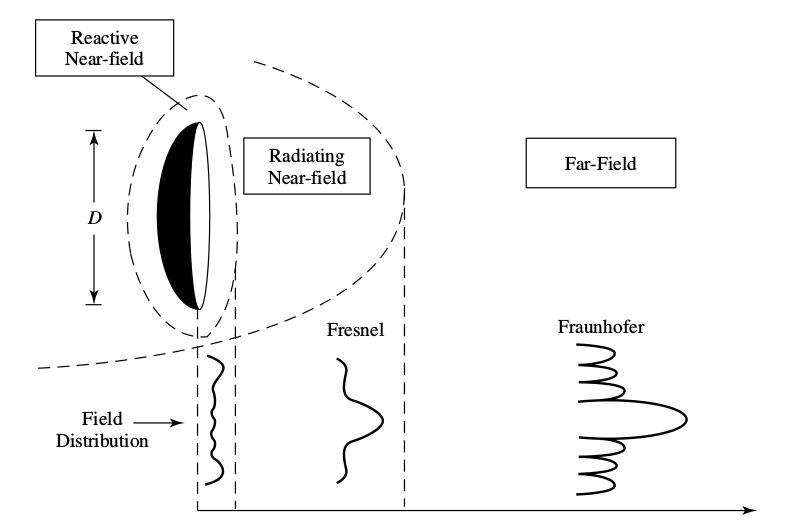
\includegraphics[width=12cm, height=9cm]{c2/amp-pattern}	   	   
	    \caption{An illustration of the various field distributions at each field zone. \emph{Source}: This figure  is reproduced from  \citep[pg. 35]{Balanis2005} 
	    but originally produced by \citep{482029}.}
	    \label{fig:amp-pattern}
       \end{figure}
  \FloatBarrier   
%%

% \begin{figure}[H]
% \centering
%  \begin{subfigure}{\columnwidth}     
%                 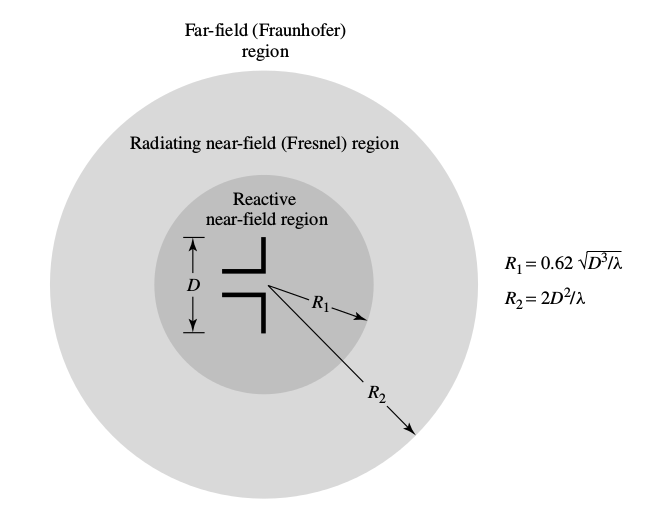
\includegraphics[width=\linewidth]{c2/field-regions2}               
%                 \caption{}                
%                 \label{fig:hg1}
%         \end{subfigure} 
%         %%
%         \begin{subfigure}{\columnwidth}
%                 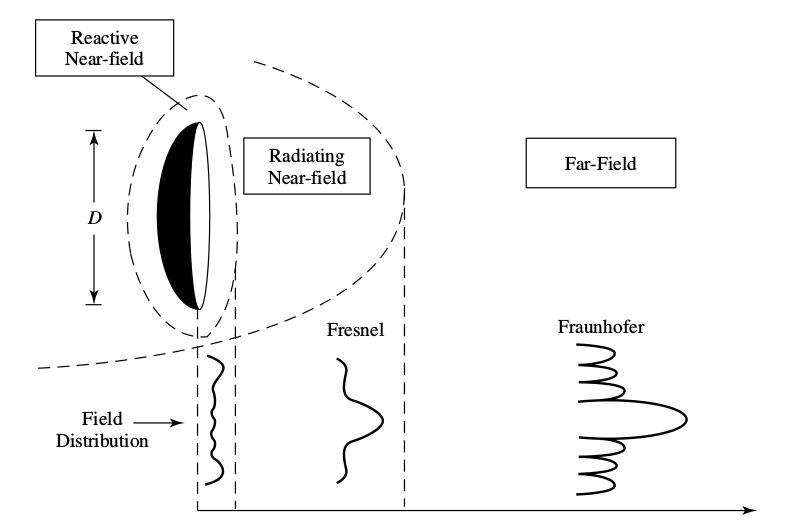
\includegraphics[width=\linewidth]{c2/amp-pattern}                
%                 \caption{}               
%                \label{fig:hg2}
%         \end{subfigure}        
%          \caption{The different field regions of an antenna. Source: This figure  is reproduced from  \citep[p. 34]{Balanis2005}.}%          
%          \label{fig:hgg}
%   \end{figure}
% \FloatBarrier


%
\subsection{Radiation Patterns}	   \label{chap2:RadiationPattern}
%
It is a visual description of the radiation properties of the antenna. The pattern of the antenna is mostly in 3D and measured in steradians, but 
can also be projected in a linear scale as shown in Fig.~\ref{fig:radiation-pattern}.  There are actually two main types of this pattern, namely:
%%
 \begin{itemize}[noitemsep]
  \item \emph{Field pattern}:- This is the amplitude of the electric field radiated by the antenna in the space coordinate. From the two plots  in Fig.~\ref{fig:radiation-pattern}, we have the maximum radiation in the vertical region and the field region can be calculated by taking the Half Power Beam Width (HPBW) of the radiation pattern. The HPBW is the angular distance at the point of $0.707$ of the maximum radiation.
  \item \emph{Power pattern}:- It is the square of the magnitude of the electric field the antenna radiates with respect to the space position. Here, the HPBW is computed at the point of $0.5$ of the maximum power radiated. The angular distance of this half power point of the maximum radiation is known as HPBW.
 \end{itemize}
%
\begin{figure}[H] %{\columnwidth}
	    \centering	
	    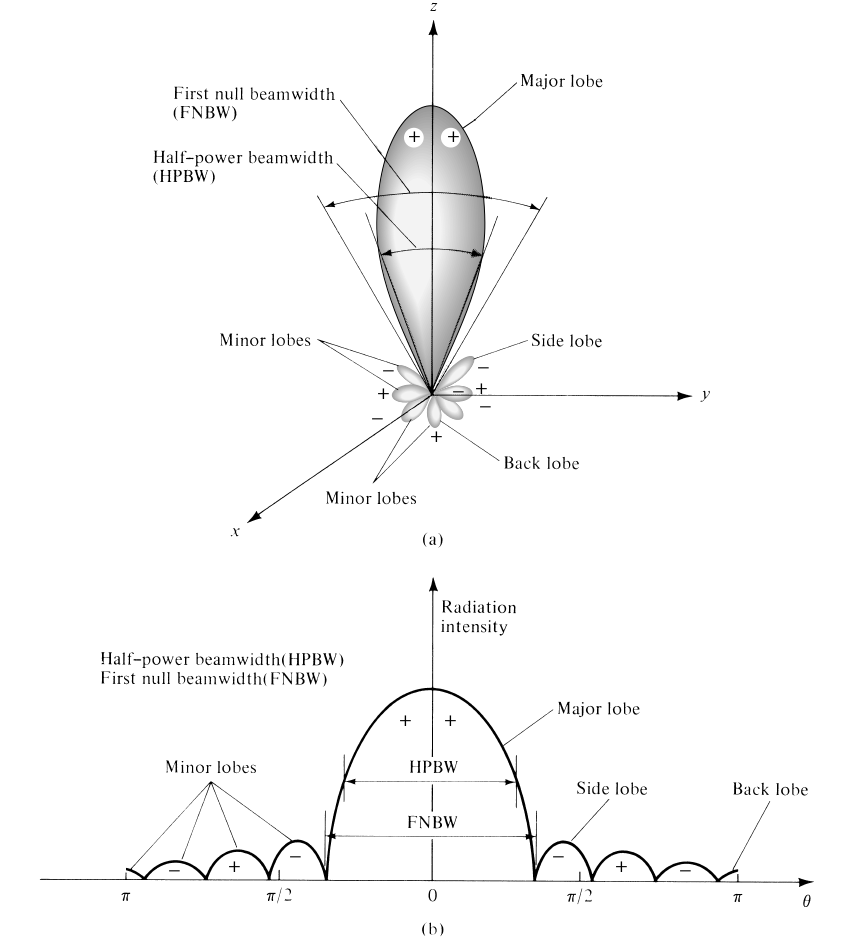
\includegraphics[width=10cm, height=12cm]{c2/radiation-pattern}
% 	    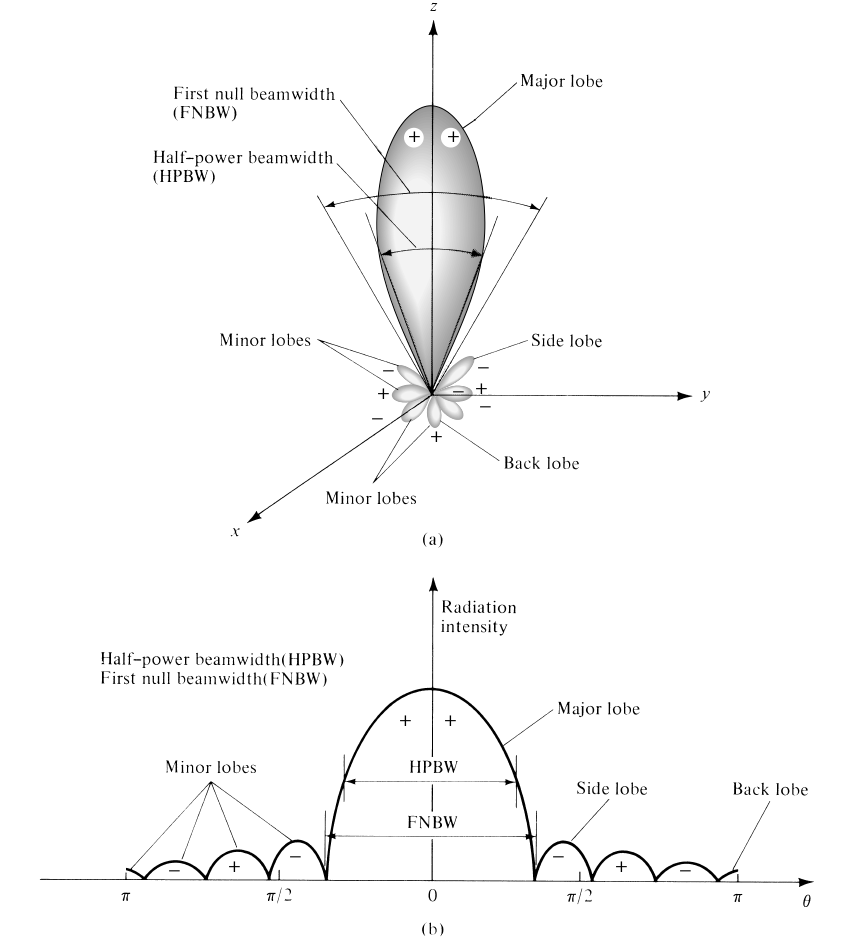
\includegraphics[width=\linewidth]{c2/radiation-pattern}	   	   
	    \caption{(a) Antenna radiation pattern showing the various lobes in angular scales.  (b) Linear projection of the pattern in (a).
	            \emph{Source}: Obtained from \citep[pg. 30]{Balanis2005}}
	    \label{fig:radiation-pattern}
       \end{figure}
  \FloatBarrier   
%%
The portion of the radiation in which the power is accommodated by the antenna is known as \emph{lobes}. We can observe from Fig.~\ref{fig:radiation-pattern} that in one
direction there is maximum power radiation and other directions there are less power radiation. The maximum power radiated in whatever direction is giving us a big lobe
of radiation known as the  \emph{major lobe}. The lobes other than the major lobe are termed  \emph{minor lobes}. These minor lobes are partitioned into \emph{side lobes} 
and \emph{back lobe}. In addition, there are certain directions where radiation drops to zero. The adjacent directions to the major lobe where the radiation drops zero
are known as \emph{null} directions. The null direction close to the major lobe is called the \emph{first null}.
%%

Depending on the shape of the radiation pattern in free space, we have different kinds, namely:
 \begin{itemize}
  \item \emph{Isotropic radiation pattern}:- As the name suggests, between halves there is equal power radiation in all directions. This type of pattern is practically not realistic 
  but the ideal case.
  \item \emph{Directional radiation pattern}:- Fig.~\ref{fig:radiation-pattern} is a typical example of directional antennas such as Cassegrain and Offset Gregorian dishes. 
  Here, we have the maximum radiation  in one direction and zero or less radiation in the other directions.
   \item \emph{Omni-directional radiation pattern}:- It is when the radiation is not in one direction but in equal orthogonal planes.
 \end{itemize}

%%
\subsection{Radiation Intensity}	   \label{chap2:RadiationIntensity}
%% 
This is the power flow per unit solid angle. It can be expressed as;
\begin{equation} \label{eq:rad_intensity}
   \Phi_{\rm rad} = r^{2}\Psi_{\rm rad}    %\frac{r^2}{2\eta}|\bm{E}(r, \theta, \phi)|^2 %   
 \end{equation} 
%  %
 where, $ \Phi_{\rm rad}$ is the radiation intensity  in $\rm Wsr^{-1}$, $\Psi_{\rm rad}$ is the intensity of the electric-field in $\rm Wm^{-2}$ and
 $r $ is the radius of the electric field component.

\subsection{Gain}	   \label{chap2:gain}
%%
The gain of an antenna is the maximum intensity in one direction to the intensity provided by the antenna if the power is radiated uniformly. Mathematically, we can define
this as;

\begin{equation}  \label{eq:gain}
   G = 4\pi\frac{ \Phi_{\rm rad}(\theta, \phi)}{P_{\rm in}}\, \mbox{(dimensionless)}    
 \end{equation} 
 %
where, $\Phi_{\rm rad}(\theta, \phi)$ is the radiation intensity in the direction $(\theta, \phi)$ and $P_{\rm in}$ is the overall accepted power. 

 
 \section{EM Wave Polarization}	   \label{chap2:WavePolarisation}
 %%
 Consider a target source emits an EM wave such that this wave is said to be unpolarized, that is, the electric field of this wave oscillates in every possible position in a plane that is perpendicular to the direction of propagation in the positive $z$ as displayed in Fig.~\ref{fig:emwave}. From Fig.~\ref{fig:emwave}, if the unpolarized wave passes through the polarizing element M1, then M1 will discard all the horizontal components and choose the components in its preferred direction. As a result, the wave that comes out is going to be polarized in the same phase as M1. 
%  a vertical polarizing element 
 %
\begin{figure}[ht]
	    \centering	    
	    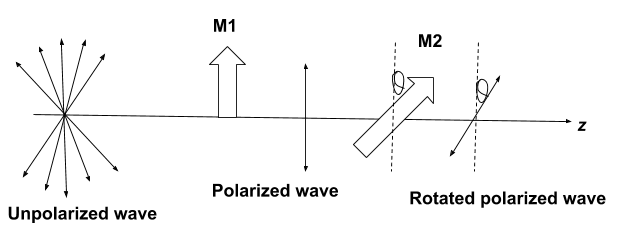
\includegraphics[width=4.2in]{c2/emwave}
	    %\vspace{5 mm}	   
	    \caption{The diagram shows how a polarizing element can polarize an unpolarized wave and also rotate the direction of incoming polarized wave.}
	    \label{fig:emwave}
       \end{figure}
  \FloatBarrier 
%%
 Note that, a polarizing element does not only polarized wave but can also rotate the wave. For instance, if the polarized wave in Fig.~\ref{fig:emwave} goes through
 the polarizer M2  at an angle $\theta$ with respect to the vertical, then M2 ignores all the wave components that are not along the preferred direction  and accepts those along
 angle $\theta$. Therefore, the output wave will still be polarized but rotated at an angle $\theta$. If $\theta = 90^\circ$, then M2 will have horizontal direction that it prefers
 by getting rid of all the vertical parts of the incoming wave. Hence, if M1 is vertical and M2 is horizontal, there would not be any wave that goes through M2.
 
 In Fig.~\ref{fig:emwave}, if we let the electric field $\vec{\xi}$, to be  polarized vertically and propagating in the direction $z$, then the magnetic field $\vec{\mathcal{B}}$ 
 is polarized horizontally (perpendicularly). Here, $\vec{\xi}$  and $\vec{\mathcal{B}}$ conform with the wave equation such that 
 the $\vec{\xi}$ units in the $(x,y)$ coordinates  of a plane-wave can be defined  as Equation~\ref{eq:wav_defn}:
 %%
\begin{subequations}
\begin{align}
\xi_{\rm x}(z, t) & =\, \xi_{\rm 1}\, \cos\{\omega t - \beta z + \varphi_{\rm x} \} \label{eq:wav_defna} \\
\xi_{\rm y}(z, t)  & =\, \xi_{\rm 2}\, \cos\{\omega t - \beta z + \varphi_{\rm y} \} \label{eq:wav_defnb}
%\phantom{\hspace{1cm}}  
 \end{align} 
 \label{eq:wav_defn}
\end{subequations}
%
%
\noindent where, the constant terms $\xi_{\rm 1}$ and $\xi_{\rm 2}$ characterise the maximum amplitude of $(x, y)$ components respectively, 
the radial frequency is $\omega = 2\pi \nu$, the ellipticity measure is expressed as $\beta = 2 \pi / \lambda$ 
and $\varphi_{\rm x}, \varphi_{\rm y}$ are phases of $\xi_{\rm x}$ and $\xi_{\rm y}$ respectively.
Equations~\ref{eq:wav_defna} and \ref{eq:wav_defnb} represent the two linearly polarized waves in the horizontal and vertical orientations respectively. Rewriting
Equation~\ref{eq:wav_defn} vectorially, we get Equation~\ref{eq:add_wav}:
%% Q5
\begin{subequations}
\begin{align}  
   \bm{\xi}(z, t)  & =\, \bm{\hat{x}}\xi_{\rm x}(z, t) + \bm{\hat{y}}\xi_{\rm y}(z, t)\\
		& =\, \bm{\hat{x}}\xi_{\rm 1}\, cos\{\omega t - \beta z + \varphi_{\rm x} \} + \bm{\hat{y}}\xi_{\rm 2}\, cos\{\omega t - \beta z + \varphi_{\rm y} \}   
 \end{align} 
 \label{eq:add_wav}
\end{subequations} 
 % 
 where, $\bm{\hat{x}},\bm{\hat{y}} = $ unit vectors in $x$ and $y$ directions. Therefore, at $z = 0$, Equation~\ref{eq:add_wav} becomes:
 
 
 %% Q6
\begin{equation}  
   \bm{\xi}(t)  = \bm{\hat{x}}\xi_{\rm 1}\, cos\{\omega t + \varphi_{\rm x} \} + \bm{\hat{y}}\xi_{\rm 2}\, cos\{\omega t + \varphi_{\rm y} \}  
  \label{eq:at_z}
 \end{equation} 
 % 
 
\noindent As clearly presented in \cite{Kraus1966}, by eliminating the time $t$ in Equation~\ref{eq:at_z}, we obtain the most general expression of an ellipse as
given in Equation~\ref{eq:gen_wav}:
%% Q7
\begin{equation}  
   a\xi_{\rm x}^2 - b\xi_{\rm x}\xi_{\rm y} + c\xi_{\rm y}^2  = 1  
  \label{eq:gen_wav}
 \end{equation} 
 
\noindent where, $a = 1/\xi_{\rm 1}^2\, \sin^{2}(\varphi)$, $b = 2\, \cos(\varphi)/\xi_{\rm 1}\xi_{\rm 2}\, \sin^{2}(\varphi)$, $c = 1/\xi_{\rm 2}^2\, \sin^{2}(\varphi)$ 
and $\varphi = \varphi_{\rm y} - \varphi_{\rm x}$.

Equation~\ref{eq:gen_wav} shows that at any specific time $t$, the locus of points characterised by the propagation of $\xi_{\rm x}$ and $\xi_{\rm y}$ will trace out this curve. In 
Equation~\ref{eq:gen_wav}, the product term $\xi_{\rm x}\xi_{\rm y}$ actually shows a rotated ellipse. Obviously,  if $\xi_{\rm 1} = 0$,  Equation~\ref{eq:add_wav} becomes linearly 
polarized in the vertical orientation, and vice versa if $\xi_{\rm 2} = 0$. When $\varphi = +90$ and $\xi_{\rm 1} = \xi_{\rm 2}$,
a \textit{left circularly polarized} wave is produced and  when $\varphi = -90$, it is known to be \textit{right circularly polarized}.


 % -------------------------------------------------------------------------------------------------------------------------------------

\subsection{Derivation of the Stokes Polarization Parameters}	   \label{chap2:sec3.1}
%
Section~\ref{chap2:WavePolarisation} dealt with fully polarized waves where, $\xi_{\rm 1},\xi_{\rm 2}$ and $\varphi$ are considered constants. 
A monochromatic (i.e. single-frequency) radiation is of that form. However, generally, in radio observation, the emission from astronomical objects expands
across a multi-frequency range and the bandwidth $\Delta \nu$, consists of incoherently polarized waves due to the superposition of independent waves of different polarizations.
In this section, we present a review of the formulation of Stokes parameters discussed by \cite{Kraus1966}. If we assume two plane waves are orthogonal and let $z = 0$ in Equation~\ref{eq:wav_defn}, 
we get  Equation~\ref{eq:plane_wav}:
% consider a pair of plane waves that are orthogonal to each other at a point in space and choosing  :
%% Q8
\begin{subequations}
\begin{align}
\xi_{x}(t) & =\, \xi_{\rm 1}(t)\, \cos\{\omega t  + \varphi_{\rm x} (t) \} \label{eq:plane_wava} \\
\xi_{y}(t)  & =\, \xi_{\rm 2}(t)\, \cos\{\omega t + \varphi_{\rm y}(t) \} \label{eq:plane_wavb}
%\phantom{\hspace{1cm}}  
  \end{align}
  \label{eq:plane_wav}
\end{subequations}
%
The time variations of $\xi_{\rm 1}(t),  \xi_{\rm 2}(t), \varphi_{\rm x} (t)$ and $\varphi_{\rm y} (t)$ are very slow compared to that of the mean frequency, 
$\nu \,(\omega = 2\pi \nu)$ which is of the order of the bandwidth $\Delta \nu$. Eliminating $\omega t $ term explicitly between Equations~\ref{eq:plane_wava} and \ref{eq:plane_wavb}
we get a similar expression in Equation~\ref{eq:gen_wav}:
%
%% Q9
\begin{equation}
  \begin{aligned}
   \frac{\xi_{\rm x}^2(t)}{\xi_{\rm 1}^{2}(t)} - 2 \frac{\xi_{\rm x}(t)\xi_{\rm y}(t)}{\xi_{1}(t)\xi_{2}(t)}\cos\, \varphi(t)  + \frac{\xi_{\rm y}^2(t)}{\xi_{2}^{2}(t)}  = \sin^{2}\, \varphi (t)
  \end{aligned}
%    \phantom{\hspace{1cm}}
  \label{eq:similar}
 \end{equation} 
%
where, $\varphi(t) = \varphi_{\rm y}(t) - \varphi_{\rm x}(t)$. Equation~\ref{eq:similar} reduces into Equation~\ref{eq:gen_wav} when monochromatic radiation is considered,
making $\xi_{\rm x}$ and $\xi_{\rm y}$ implicitly time dependent.

In order to measure the intensity of a radio wave, we compute the average per the time of observation and  assume the time taken to be infinite because 
it takes a lot time to oscillate per cycle. The time average for Equation~\ref{eq:similar} is therefore represented as:
%
%% Q10
\begin{equation}
  \begin{aligned}
   \frac{\langle \xi_{\rm x}^{2}(t)\rangle}{\xi_{\rm 1}^{2}} - 2 \frac{\langle \xi_{\rm x}(t)\xi_{\rm y}(t)\rangle}{\xi_{\rm 1}\xi_{\rm 2}}\cos\, \varphi  +
   \frac{\langle \xi_{\rm y}^{2}(t)\rangle}{\xi_{\rm 2}^{2}}  = \sin^{2}\, \varphi 
   \end{aligned}
%    \phantom{\hspace{1cm}}
  \label{eq:time_avg}
 \end{equation} 
%
where the symbol $\langle \, \rangle$ denotes the time average and 
%
%% Q11
\begin{equation}
  \begin{aligned}
   \langle \xi_{\rm i}(t)\xi_{\rm j}(t)\rangle = \lim_{T \to \infty} \int\limits_0^T \, \xi_{\rm i}(t)\xi_{\rm j}(t) dt, \quad i, j = x, y
  \end{aligned}
%    \phantom{\hspace{1cm}}
  \label{eq:avg_wav}
 \end{equation} 
%
% 
Multiply Equation~\ref{eq:time_avg} by $4\xi_{\rm 1}^{2}\xi_{\rm 2}^{2}$  and then use Equation~\ref{eq:avg_wav} to compute the average terms in Equation~\ref{eq:time_avg} to get:

%% Q14 
\begin{equation}
  \begin{aligned}
   2\xi_{\rm 1}^{2}\xi_{\rm 2}^{2} - (2\xi_{\rm 1}\xi_{\rm 2}\, \cos\, \varphi )^2 + 2\xi_{\rm 1}^{2}\xi_{\rm 2}^{2} = (2\xi_{\rm 1}\xi_{\rm 2}\, \sin\, \varphi )^2
  \end{aligned}
%    \phantom{\hspace{1cm}}
  \label{eq:wavq}
 \end{equation} 
% %
Representing Equation~\ref{eq:wavq} in perfect square form, we add and subtract $\xi_{1}^{4} + \xi_{2}^{4}$ to get:
%% Q15
\begin{equation}
  \begin{aligned}
   (\xi_{\rm 1}^{2} + \xi_{\rm 2}^{2})^2 - (2\xi_{\rm 1}\xi_{\rm 2}\, \cos\, \varphi )^2 - (\xi_{\rm 1}^{2} - \xi_{\rm 2}^{2})^2 = (2\xi_{\rm 1}\xi_{\rm 2}\, \sin\, \varphi )^2
  \end{aligned}
%    \phantom{\hspace{1cm}}
  \label{eq:deduce}
 \end{equation} 
% %
We can deduce the intensities from Equation~\ref{eq:deduce}:
%% Q16
\begin{subequations}\label{eq:stok}
\begin{align}
P_{\rm I}  & =\,  \xi_{\rm 1}^{2} + \xi_{\rm 2}^{2}	 	\label{eq:stoka} \\
P_{\rm Q} & =\,  \xi_{\rm 1}^{2} - \xi_{\rm 2}^{2} 		\label{eq:stokb} \\
P_{\rm U}  & =\,  2\xi_{\rm 1}\xi_{\rm 2}\, \cos\, \varphi 		\label{eq:stokc} \\ 
P_{\rm V}  & =\,  2\xi_{\rm 1}\xi_{\rm 2}\, \sin\, \varphi  	\label{eq:stokd} 
%\phantom{\hspace{1cm}}
\end{align}
\end{subequations}
%

% \noindent Equation~\ref{eq:stok} is then expressed as:
% % % Q17
% \begin{equation}
%   \begin{aligned}
%    I^2 = Q^2 \, + \, U^2 \, + \, V^2
%   \end{aligned}
% %    \phantom{\hspace{1cm}}
%   \label{eq:intensity}
%  \end{equation} 
%  
\noindent  $I, Q, U\, \textrm{and}\, V$ in Equation~\ref{eq:stok} are the real quantities of Stokes parameters with $I$ being the total intensity. 
 The parameter $Q$ characterises the linear horizontal or vertical polarization; that of $U$ characterises the amount of linear $\pm 45^\circ$ polarization 
 and $V$ represents circular polarization. We can calculate the degree of polarization $P_{\rm {deg}}$, for a given state of polarization:
%% Q18
\begin{equation}
  \begin{aligned}
   P_{\rm deg} = \frac{I_{\rm pol}}{I_{\rm tot}} = \frac{(Q^2 \, + \, U^2 \, + \, V^2)^{1/2}}{I}, \quad 0 \leq P_{\rm deg} \leq 1
  \end{aligned}
   \phantom{\hspace{1cm}}
  \label{eq:q18}
 \end{equation} 
% %
However, ignoring the time average approach and expressing Equations~\ref{eq:plane_wava} and~\ref{eq:plane_wavb} in terms of complex amplitudes to obtain Equation~\ref{eq:q19}:
% \noindent where, $I_{pol}$ is the intensity of the sum of the polarization components and $I_{tot}$ is the total intensity of the signal. $P_{deg} = 1$ 
% relates to completely polarized light, $P_{deg} = 0$ relates to unpolarized light and $0 < P_{deg} < 1$ relates to partially polarized light.
% 
% \noindent The Stokes parameters can also be obtained by ignoring the time average approach and expressing Equations~\ref{eq:plane_wava} and~\ref{eq:plane_wavb} in terms of complex amplitudes:
%% Q19
\begin{subequations}
\begin{align}
\xi_{\rm x}(t) & =\, \xi_{\rm x}\, \exp\{i\omega t \}   \label{eq:q19a} \\
\xi_{\rm y}(t) & =\, \xi_{\rm y}\, \exp\{i\omega t \} 	\label{eq:q19b}
\end{align}
\label{eq:q19}
\end{subequations}
% %
where $\xi_{x} = \xi_{1}\, \exp\{i \varphi_{x} \}$ and $\xi_{y} = \xi_{2}\, \exp\{i \varphi_{y} \}$ are  the complex amplitudes. 
The Stokes polarization parameters from these complex amplitudes are:
% %% Q20
\begin{subequations}
%\begin{eqnarray}
\begin{align}
P_{\rm I}  & =\,  \xi_{\rm x}\xi_{\rm x}^{*} + \xi_{\rm y}\xi_{\rm y}^{*}	 	\label{eq:q20a} \\
P_{\rm Q}  & =\,  \xi_{\rm x}\xi_{\rm x}^{*} - \xi_{\rm y}\xi_{\rm y}^{*}		\label{eq:q20b} \\
P_{\rm U}  & =\, \xi_{x}\xi_{y}^{*} + \xi_{y}\xi_{x}^{*} 		\label{eq:q20c} \\ 
P_{\rm V}  & =\,  i(\xi_{\rm x}\xi_{\rm y}^{*} - \xi_{\rm y}\xi_{\rm x}^{*})		\label{eq:q20d} 
\end{align}
\label{eq:q20}
%\phantom{\hspace{1cm}}  
%\end{eqnarray}
\end{subequations}
% %
% 
These Stokes terms can be used to describe the full polarization state of a signal, for instance, the foregrounds are mostly presented in Stokes parameters.
Chapter~\ref{Chapter4} gives a further detail on how to formulate the Stokes parameters in 
terms of the column matrix to obtain not only measurable intensities but also observables too.
% For a more general discussion on wave polarization see \citep{bkk8,bkk7,bkk9,bkk10,bkk11}. 
% % 
% In short, when an antenna intercepts an EM wave then the polarized instrument depends on the position of observation.
% \noindent Substituting Equations~\ref{eq:q19a} and ~\ref{eq:q19b} into Equation~\ref{eq:q20}, we reproduce the expression in Equation~\ref{eq:q16}. 
% 
% The Stokes parameters give a full characterisation of any polarization state of a plane wave. In Chapter~\ref{Chapter4}, we discuss further on how to formulate the Stokes parameters in
% terms of the column matrix to obtain not only measurable intensities but also observables too. For a more general discussion on wave polarization see \citep{bkk8,bkk7,bkk9,bkk10,bkk11}. 
% 
% In short, an EM wave received by an antenna consists of both electric and magnetic fields. If we are to track the curve traced by the tip of the
% electric field vector, in some fixed location in space, we will get, as time varies, a curve referred to as the polarization ellipse. 
% Also, for a specified location we would generally get different curves, that is to say, the antenna polarization is dependent upon the direction of observation.
%  %
% % -------------------------------------------------------------------------------------------------------------------------------------

 
  \section{Antenna Arrays}	   \label{chap2:sec4}
  %
  Array antenna (also known as interferometer) is the connection of at least two spatially distributed  antennas used to measure or direct the radiation intensity of a source 
  towards a desired angular sector in order to have an improved performance over a single antenna. One unique property of an interferometer is that the beam pattern can be changed when we 
  electronically steer or scan the antenna elements towards some other direction by changing their relative amplitudes and phases. 
  This operation can not be done with a single dish since the beam pattern remains constant. 
%   The use of an array for an observation
%   gives us the opportunity to impose a particular desired array pattern without changing its physical dimensions. Furthermore, by manipulating the received signals from the individual antenna elements in different ways, we can achieve many signal processing
% functions, such as spatial filtering \citep{2009arXiv0910.2865A,2000astro.ph..8239L,2008ISTSP...2..613W}, interference suppression 
% \citep{2008ISTSP...2..670B,2010arXiv1008.5066L,2005RaSc...40.5S11M}, gain enhancement \citep{2008arXiv0809.0208Y}, 
% target tracking \citep{2015PASA...32...17W,2015A&A...573A..99D}, etc.
% %%

% -------------------------------------------------------------------------------------------------------------------------------------

%  (\theta,\phi) = (\vartheta,\varphi)
%
\subsection{Mathematical Formulation of Antenna Array}	    \label{chap2:sec4.1}
%
\theo{
Consider $N$ antenna elements with corresponding radiated electric field $\bar{E}_{k}(\theta,\phi)\mid_{k = 1, 2,3, \ldots, N}$ such that the
angle of elevation and azimuth of these elements are defined  within the range of $-90^{\circ} \leq \theta \leq 90^{\circ}$
and $-180^{\circ}  \leq \phi  \leq 180^{\circ}$ respectively. Then, the overall electric field $\bar{E}(\theta,\phi)$ can be expressed as:
% % Q21
\begin{equation}
  \begin{aligned}
   \bar{E}(\theta,\phi) = \sum_{n = 1}^{N} \, w_{n} \bar{E}_{n}(\theta,\phi)\exp \{i\xi \psi_{n}(\theta,\phi) \}
  \end{aligned}
%    \phantom{\hspace{1cm}}
  \label{eq:q21}
 \end{equation} 
%
where, the element location is $\psi_{n} = x_{n}\sin\, \theta \cos \, \phi + y_{n}\sin\, \theta \sin \, \phi + z_{n}\cos \, \theta $, $\xi = \frac{2\pi}{\lambda}$ is the wavenumber,
$w_{n}|_{n = 1, 2, 3, \ldots, N}$ are the elements complex weights. If the antenna elements are identical, Equation~\ref{eq:q21} becomes;
%
%% Q22
\begin{equation}
  \begin{aligned}
   \bar{E}(\theta,\phi) = \bar{E}_{1}(\theta,\phi)\, \sum_{n = 1}^{N} \, w_{n} \exp \{i\xi \psi_{n}(\theta,\phi) \}
  \end{aligned}
%    \phantom{\hspace{1cm}}
  \label{eq:q22}
 \end{equation} 
%
where $\bar{E}_{1}(\theta,\phi)$ is the element factor and $ \sum_{n = 1}^{N} \, w_{n} \exp \{i\xi \psi_{n}(\theta,\phi) \}$ is the array factor (AF). Equation~\ref{eq:q22}
characterises the \textit{array pattern multiplication}. Assuming we place $N$ antenna elements uniformly linear on a particular 
axis with uniform spacing $n\Delta|_{n = 0, 1, 2, 3,\ldots, N - 1 }$, then:
%
%% Q23
\begin{equation}
  \begin{aligned}
   AF = \sum_{n = 0}^{N-1} \, w_{n} \exp \{i\xi n\Delta \cos\, \theta \}
  \end{aligned}
%    \phantom{\hspace{1cm}}
  \label{eq:q23}
 \end{equation} 
%
where $w_{n} = \exp \{-i\xi n\Delta \, \cos \, \theta_0 \}$. Hence, substituting this into  Equation~\ref{eq:q23}, we get:
%%
%
\begin{equation}
  \begin{aligned}
   AF = \sum_{n = 0}^{N-1} \, (\exp \{i\gamma\})^n, \quad \gamma = \xi\Delta(\cos \theta - \cos \theta_{0})
  \end{aligned}
%    \phantom{\hspace{1cm}}
  \label{eq:af23}
 \end{equation} 
%%
%
% (\exp \{i\gamma\})^n$. letting $\gamma = \xi\Delta(\cos \theta - \cos \theta_{0})$, 
%
\noindent From the geometrical progression theory, we can recall that: 
$$ \sum_{n = 0}^{\infty}\alpha^n = \frac{1}{1 - \alpha}, \alpha \neq 1 \, \mathrm{and} \, \sum_{n = 0}^{N - 1}\alpha^n = \frac{1 - \alpha^N}{1 - \alpha}, \alpha \neq 1$$.
%%
\noindent Applying these two theories to Equation~\ref{eq:af23}, we obtain Equation~\ref{eq:q24}:
% Q24
\begin{subequations}\label{eq:q24}
 \begin{align}
   AF & =\, \frac{1 \, - \, \exp \{ iN\gamma\}}{1 \, - \, \exp \{ i\gamma\}}	\label{eq:q24a}\\ 
     & =\, \frac{\exp \{ iN\gamma/ 2\}}{\exp \{ i\gamma/ 2\}}\frac{\exp \{ iN\gamma/ 2\} - \exp \{ -iN\gamma/ 2\}}{\exp \{ i\gamma/ 2\}-\exp \{ -i\gamma/ 2\}}	\label{eq:q24b}\\ 
      & =\,  \exp \{ i(N - 1)\gamma / 2\}\,\frac{\sin \, (N\gamma/2)}{\sin \, (\gamma/2)} 	\label{eq:q24c}
%        & =\, \exp \{i(N -1)\xi\, \Delta/2 ( \cos\, \theta -  \cos\, \theta_0) \}\,\frac{\sin \, \{ \xi N (\Delta/2)( \cos\, \theta -  \cos\, \theta_0) \}}{
%        \sin \, \{ \xi (\Delta/2)( \cos\, \theta -  \cos\, \theta_0) \}} \label{eq:q24d}
 \end{align}  
 \end{subequations}
%
%
\noindent Since $\sin(Nx)/\sin(x)$ behaves like $N\sinc(x)$, ignoring the phase factor produces Equation~\ref{eq:q26}:
%
%
% %% Q25
% \begin{equation}
%   \begin{aligned}
%    AF = \frac{1}{N} \,  \frac{\sin \, \{ \xi N (\Delta/2)( \cos\, \theta -  \cos\, \theta_0) \}}{
%        \sin \, \{ \xi (\Delta/2)( \cos\, \theta -  \cos\, \theta_0)\}}
%   \end{aligned}
%    \phantom{\hspace{1cm}}
%   \label{eq:q26}
%  \end{equation} 
% %
%
% Q25
\begin{equation}
  \begin{aligned}
   AF = N\sinc  \gamma/2
  \end{aligned}
%    \phantom{\hspace{1cm}}
  \label{eq:q26}
 \end{equation} 
 %
 %
% 
\noindent Therefore, the maximum value of Equation~\ref{eq:q26} occurs when $\gamma = 0$, making $AF = N$. 
% -------------------------------------------------------------------------------------------------------------------------------------
}  % @@@@@@@@@@@@@@@@@@@@@@@@@@@

%
\subsection{Beam-forming}	  	\label{chap2:Beam-forming}
%

The combination of multiple signals with different complex weights from different receiving antenna elements forms a new radiation pattern.
This technique is known as \textit{beam-forming} and can be done in analogue components such as LOFAR with high-band antennas (HBA)
or after the signal is digitised, such as in the LOFAR stations. The algorithms used to generate the technique can be classified into \textit{coherent},
\textit{incoherent} and \textit{multi-pixel beam-former} methods. The application of coherent beam-forming allows a narrow beam to be formed and, 
therefore provides a higher gain which is very useful, for example, during pulsar observation.  Coherent beam-forming increases the sensitivity in narrow FoV.
Unlike coherent beam-forming, incoherent beam-forming does not affect FoV but increases the overall sensitivity. This kind of algorithm is very useful 
when searching for rare events where the location of occurrence is not known. The application of a multi-pixel beam-former like the 
\enquote{Giant Metre wave Radio Telescope} (GMRT\footnote{\url{ http://gmrt.ncra.tifr.res.in/}}) integrates the 
sensitivity of the other two methods by using a \enquote{recorded base-band data} \citep{2012MNRAS.427L..90R} where there is a direct receiving of raw voltage samples 
from the interferometer into an array of storage disks. The technique used for observing pulsars mostly in extended sources can be made more efficiently, 
using the multi-pixel beam-former approach as shown in \cite{deng2017observing}.


% % -------------------------------------------------------------------------------------------------------------------------------------
% 
% %
\subsection{Types of Radio Arrays}	  \label{chap2:sec4.3}
%
In this subsection, we discuss the main types of antenna receiving elements that can be used for radio interferometric observations. The advantages and disadvantages are also
discussed.
%
% -------------------------------------------------------------------------------------------------------------------------------------

\subsubsection{Phased-Array Feeds (PAFs)}	   \label{chap2:sec4.3.1}
%
Generally, a single dish has one pixel and only records the total power captured within its primary beam at any given time. We can produce an image by pointing the single
beam at different directions and then project the output on a sky grid. PAF is a feed design of an antenna dish that consists of elements at reflector focus. 
It is mainly made up of antennas, hardware for signal processing and amplifiers.
% A feed design for a dish, which incorporates multiple feeds instead of the single \enquote{pixel} feed, is referred to as a \enquote{Phased-Array Feed} (PAF). 
This new technology in radio astronomy is the same as having several arrays pointing at different places simultaneously. Its feed
horn is electrically large and collects nearly all focused signal energy. Imaging with an array of multi-beam antennas gives a good resolution and increase in FoV. 
This increase in FoV comes at a cost of each receiving element requiring its own isolated analogue front-end and digital back-end, making the feed more expensive.
This is a new technology undergoing development and currently, PAFs have a higher system temperature and more limited analogue bandwidth than a feed with single pixel.
Even though calibration and how to handle the big data of these new instruments are some of the challenges, their design and ongoing state of development serve as a pathfinder for the SKA \citep{6051207}. 
Some of the PAF-based arrays are the \enquote{Aperture Tile In Focus} (APERTIF\footnote{\url{https://www.astron.nl/astronomy-group/apertif/apertif}}) \citep{oosterloo2009apertif} 
which is an upgrade on  \enquote{Westerbork Synthesis Radio Telescope} (WSRT) and 
\enquote{Australian Square Kilometre Array Pathfinder} (ASKAP\footnote{\url{ http://www.atnf.csiro.au/projects/askap/index.html}}) \citep{johnston2009science}
as displayed in Fig.~\ref{fig:pafs}.
%%
%	+++++++++++++++++++++++++++++++++++++++++++
%	PAFs
%	++++++++++++++++++++++++++++++++++++++++++++
%
\begin{figure}[ht]
	    \centering	    
	    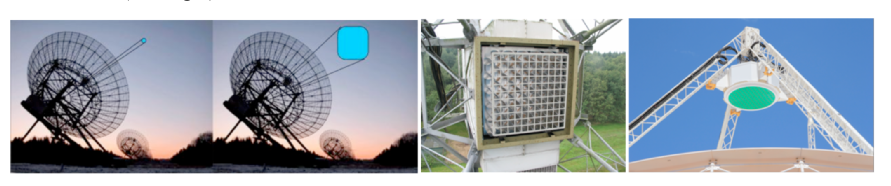
\includegraphics[width=5.8in]{c2/wsrt}
	    %\vspace{5 mm}	   
	    \caption{PAFs showing the wide gain in the FoV. The third image from the left is the installation of APERTIF on WSRT. 
	    The last image from the left displays the PAFs fixed on ASKAP.  \emph{Source}: Reproduced from \cite{garrett2013radio}.
	    }
	    \label{fig:pafs}
       \end{figure}
  \FloatBarrier 
  %
% -------------------------------------------------------------------------------------------------------------------------------------

%
\subsubsection{Transiting Arrays}	   \label{chap2:sec4.3.2}
%
Unlike a dish that can track a particular point in the sky over many hours, a transiting array has elements with limited mobility and allows the sky
to drift through the primary beam of the elements. Its feed has an effective primary beam which is large compared to that of a dish.
As a source enters into the beam, it starts with a small apparent flux, then gradually increases until the source peaks at the zenith. It then decreases as it moves 
across the beam side lobes until it finally sets at the horizon. Some of the  transiting arrays are \enquote{Precision Array for Probing the Epoch of Reionization} (PAPER)
\citep{parsons2010precision},  \enquote{Long Wavelength Array} (LWA) \citep{ellingson2013design}, Medicina Northern Cross and 
the \enquote{Murchison Widefield Array} (MWA\footnote{\url{ http://www.mwatelescope.org/}}) \citep{2009IEEEP..97.1497L} as shown in Fig.~\ref{fig:paper}. Note that
some of the transit arrays such as CHIME, Tianlai, HIRAX, and UTMOST\footnote{\url{https://astronomy.swin.edu.au/research/utmost/}} use collecting elements.
There are obvious cost advantages to building an array with no moving parts. Such arrays have wide FoV and can have the individual elements
placed close together. This allows for large-scale structure experiments, such as Epoch of Reionization (EoR) and BAO studies. 
The disadvantages compared to dishes create a new challenge for calibration and imaging. The individual elements are less sensitive compared to a dish, so more
elements are needed, which requires larger correlator systems. In addition, as the sky transits, the apparent flux of sources changes, so the primary beam must be well known in order 
to get back to the intrinsic flux of the sky. Depending on the scale of the primary beam, a transiting array has a set amount of time per day in which a
section of the sky can be observed. This means that a deep integration of a region of sky is not possible without observing it for many days.
%
%
%	+++++++++++++++++++++++++++++++++++++++++++
%	Transiting Arrays
%	++++++++++++++++++++++++++++++++++++++++++++
%
\begin{figure}[ht]
\centering	    
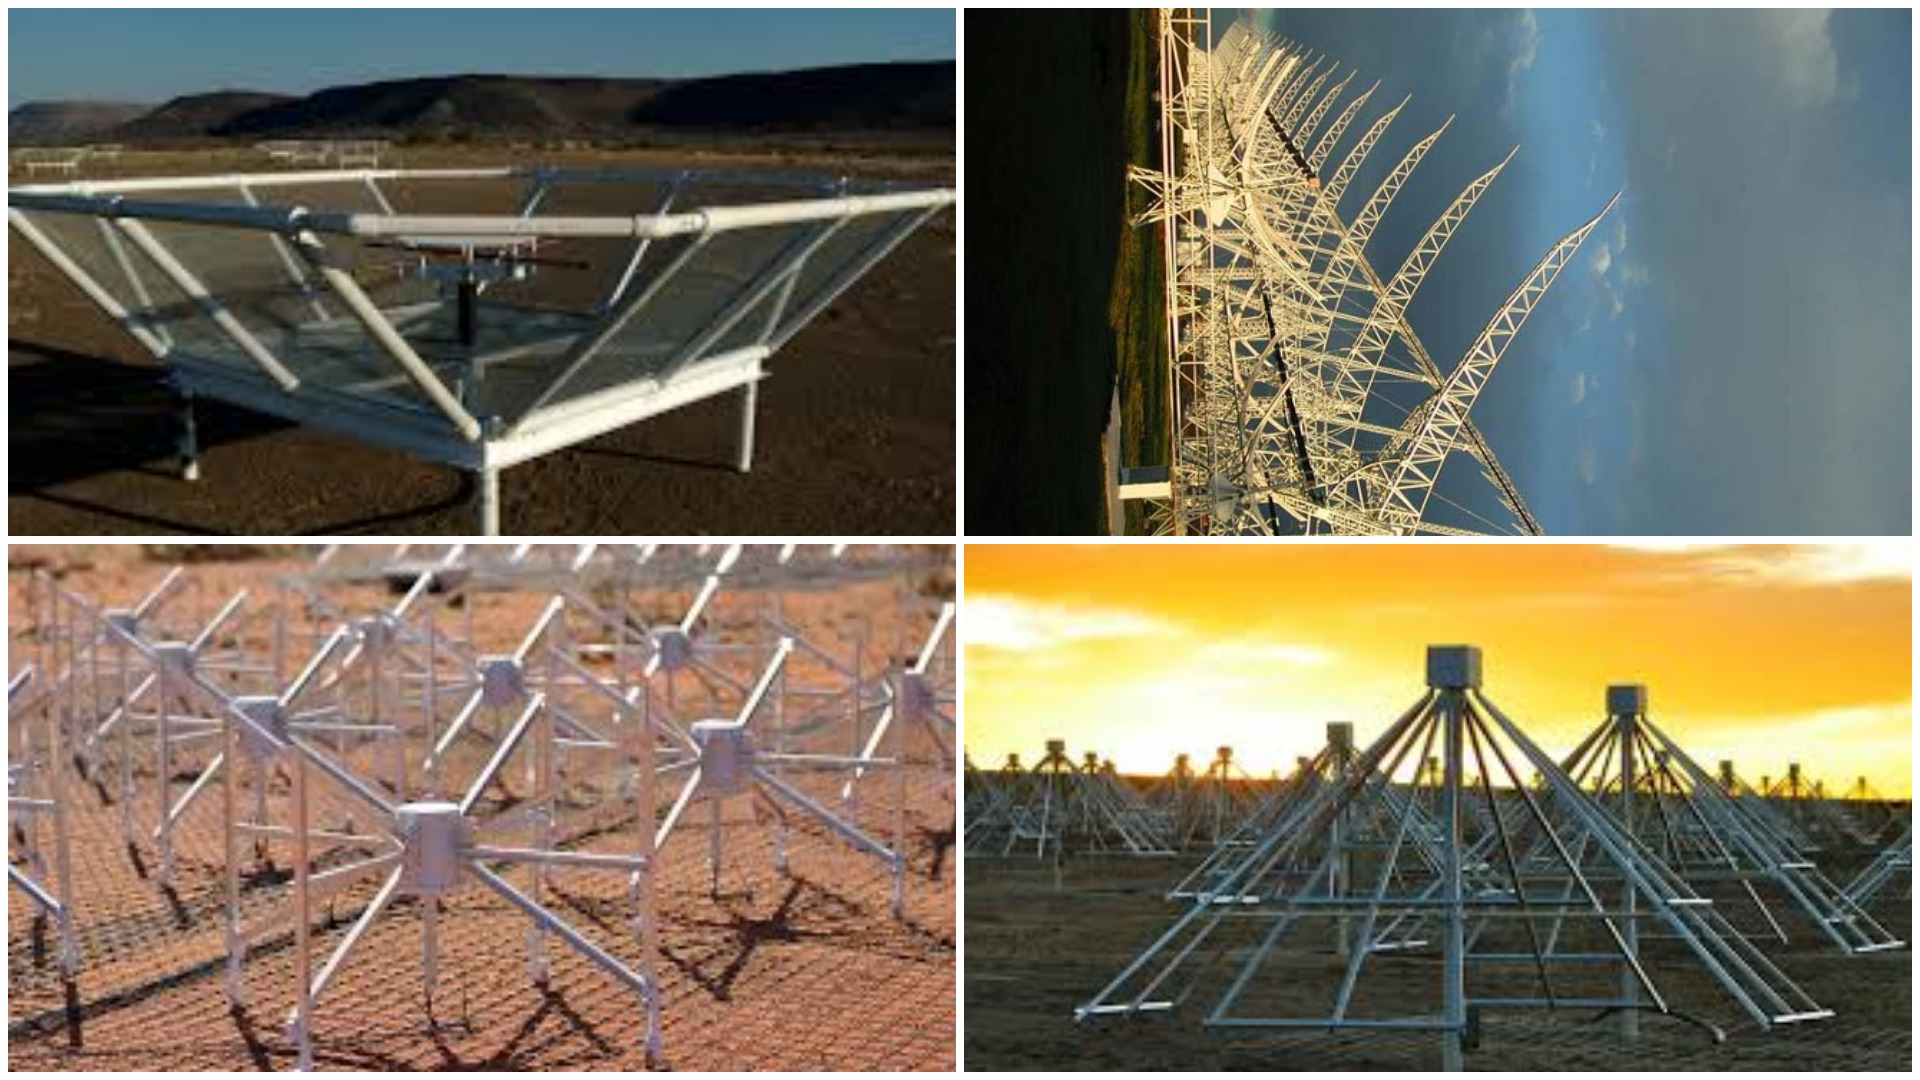
\includegraphics[width=5.8in]{c2/paper-lwa-mwa-cross}
%\vspace{5 mm}	   
\caption{Transiting Arrays:- PAPER (top-left), LWA (bottom-left),  Medicina Northern Cross(top-right) and MWA (bottom-right).}
\label{fig:paper}
\end{figure}
  \FloatBarrier 
  %
  
  % -------------------------------------------------------------------------------------------------------------------------------------

  
\subsubsection{Aperture Arrays}	   \label{chap2:sec4.3.3}
%
We can convert a transiting array into a digital dish to form an \textit{aperture array}. This makes it possible to point the digital dish in many directions of the sky 
simultaneously. The idea with an aperture array is that by updating the beamforming weights, the beam of the aperture array can track a region of the sky. The aperture array takes
advantages from both dishes and transiting arrays. The main cost is the analogue and digital electronics to build such an array. For this reason, aperture arrays are 
mainly used for low-frequency science, such as LOFAR as in Fig.~\ref{fig:lofar} and the future SKA-LOW shown in Fig.~\ref{fig:daa}, as the Dense Aperture Array (DAA) 
components are cheaper. With improved technology, the price of higher frequency components will make it possible to increase the observable frequency. A second issue with aperture arrays is that the primary beam changes, depending on pointing location 
and frequency. As the beam is a weighted sum of all the individual elements there is limited precision to the beam shape. There is a design difference of sparse 
and dense aperture arrays. When the elements of the aperture array are placed closer than $\lambda/2$ observing wavelength the array is \textit{dense}. The array is
fully sampling the wavefront and there are no beam artefacts, such as \textit{grating lobes} (a type of side lobe) which introduces significant structure into the beam. 
If the elements are further apart than $\lambda/2$ then these side lobes structures appear and limit the sensitivity and FoV. For a single observing frequency,
designing an aperture array is simple as all the elements are spaced at $\lambda/2$. However, for wide-band arrays, if the elements are placed at $\lambda_{i}/2$
for a wavelength $\lambda_{i}$ , then for any wavelength $< \lambda_{i}$ the array configuration under-samples that observing wavelength and introduces large grating lobes. 
Therefore, a balance between observing bandwidth, cost and dense versus sparse trade-off must be made during the array design.



%	+++++++++++++++++++++++++++++++++++++++++++
%	Aperture Arrays
%	++++++++++++++++++++++++++++++++++++++++++++
%
\begin{figure}[ht]
    \centering	    
    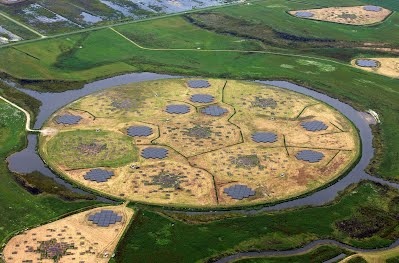
\includegraphics[width=4.2in]{c2/lofar}
    %\vspace{5 mm}	   
    \caption{Aperture Array:- LOFAR.}
    \label{fig:lofar}
\end{figure}
  \FloatBarrier 
  %
%
%	+++++++++++++++++++++++++++++++++++++++++++
%	future Aperture Array
%	++++++++++++++++++++++++++++++++++++++++++++
%
\begin{figure}[ht]
    \centering	    
    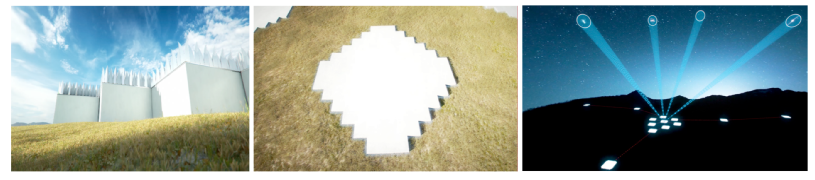
\includegraphics[width=5.8in]{c2/DAA}
    %\vspace{5 mm}	   
    \caption{SKA-2 Dense Aperture Arrays precursor telescope.}
    \label{fig:daa}
\end{figure}
  \FloatBarrier 
%   %
A more detailed discussion on radio arrays can be seen in \cite{techreport-minimal3}.
%

  % -------------------------------------------------------------------------------------------------------------------------------------
 
  \section{Power gained from Radio Sources}	   \label{chap2:sec5a0}
  
The receivers of a radio telescope are very sensitive to the orientation state of the incoming radiation. More generally, in radio astronomy, two receivers are 
attached to each receiving feedhorn, with a splitter feeding horizontally polarized radiation to one receiver
and vertically polarized radiation to the other. The sum of what is obtained in each polarization is known as the \emph{total intensity}. In each polarization, 
the power $P_{w}$ received per unit bandwidth from an element of solid angle of the sky is defined as Equation~\ref{eq:pwr};
%%
\begin{equation} \label{eq:pwr}
P_{w} = \frac{1}{2}A_{e}\iint\limits_{\varOmega}\, B_{s}(\theta,\phi)P_{n}(\theta,\phi)\, d\varOmega 
\end{equation}

\noindent where $A_{e} = $ effective aperture (collecting area) of antenna $\mathrm{[m^{-2}]}$,\\
$B_{s}(\theta,\phi) = $ brightness distribution of radio emission across the sky $\mathrm{[Wm^{-2}Hz^{-1}sr^{-1}]}$,\\
$P_{n}(\theta,\phi) =$ normalised power (beam) pattern of the antenna,\\
$d\varOmega = \sin\theta\, d\theta d\phi$, element of solid angle $\mathrm{[sr]}$.
%%

 In radio astronomy, what we are mostly interested in is the integral of the brightness over a radio source say $S$. The notation $S$ defined in Equation~\ref{eq:flx}
 is the \emph{flux density}: 
%%
\begin{equation} \label{eq:flx}
 S = \iint\limits_{source} \, B_{s}(\theta,\phi) \, d\varOmega
\end{equation}
%%

\noindent Consider the radio source is observed with a radio telescope with the power pattern $P_{n}(\theta, \phi)$, then, 
the observed flux density is computed by the product of the integral of the brightness distribution and the antenna beam pattern:

%%
\begin{equation} \label{eq:flxa}
 S_{0} = \iint\limits_{source} \, B_{s}(\theta,\phi)P_{n}(\theta,\phi) \, d\varOmega
\end{equation}
%%

\noindent In Equation~\ref{eq:flxa}, if we have a radio point source at the phase centre of the beam, then, $P_{n}(\theta,\phi)\simeq 1$ and $S \simeq S_0$, but if the 
source is extended with simple geometry, then simple analytic function will enable $S_0$ to be corrected and this is discussed in the \cite{Gaylard2012} technical report. 
The SI unit of flux density is usually expressed in $\mathrm{Wm^{-2}Hz^{-1}}$. Nevertheless, the radio emission is not very strong because it is emitted from a distant radio source,
and the unit is mostly expressed as Jansky [Jy] which is named after the radio astronomer Karl Jansky. Here,  $1 \mathrm{Jy} \equiv \mathrm{10^{-26} Wm^{-2}Hz^{-1}}$.


%  \section{Brightness Temperature and Antenna Temperature}	   \label{chap2:sec5a}
%  
%  Radio astronomy can be seen as a blend of astronomy and the fundamental of electric circuit theory. Therefore, a
%  radio telescope can be considered as an electric circuit and the source being observed
% can be taken as a resistor at a specific temperature connected to the first amplifier in the receiver
% (by radio waves rather than by wires). For some astronomical sources, the temperature that is determined can be 
% meaningful as a physical temperature or not, depending on the radiation mechanism involved,
% and we therefore, refer to the \emph{brightness temperature} $T_{B}$ for these emitters. For instance, the gas producing the emission may have a physical temperature of  $< 200$ K, but
% the very intense stimulated emission of the maser could have a $T_{B}$ of $1012$ K. $T_{B}$ can be related to the Rayleigh-Jeans law:
% %%
% \begin{equation} \label{eq:ray}
%  T_{B} = \frac{\lambda^{2}}{2k_{B}\varOmega}S \,\mathrm{[WHz^{-1}]}
% \end{equation}
% 
% where $\lambda$ the wavelength, $k_{B}$ the Boltzmann constant, $\varOmega$ the beam solid angle and $S$ the flux density of a source, all in mks units.  
% For a Gaussian beam, its solid angle $\varOmega$  is related to the HPBW $\theta$ by:
% %%
% \begin{equation} \label{eq:omega}
%  \varOmega = \frac{\pi\theta^2}{4\ln 2} %\mathrm{[radians]}
% \end{equation}
% 
% If we observe the radiation from a discrete source which has an effective temperature $T_{B}$ and subtends a solid
% angle $\varOmega$, the source flux density is simply the product of the brightness and the source solid
% angle:
% 
% \begin{equation} \label{eq:src}
%  S = \frac{2k_{B}T_{B}\varOmega}{\lambda^{2}}\, \mathrm{[Wm^{-2}Hz^{-1}]}
% \end{equation}
% %%
% 
% More generally, if the temperature distribution over the emitter is not uniform, the flux density becomes the integral of the temperature distribution over the object:
% \begin{equation} \label{eq:gsrc}
%  S = \frac{2k_{B}}{\lambda^{2}}\iint\limits_{source} T_{B}(\theta, \phi)\, d\varOmega\, \mathrm{[Wm^{-2}Hz^{-1}]}
% \end{equation}

 
  \section{Basic Concepts of Radio Interferometry}	   \label{chap2:Interferometry}
  %
  
  Radio Interferometry is the process of using at least two radio elements to observe astronomical sources. When we synthesize the signals
  from the array along with the electronics we term it the interferometer. For a single telescope, the angular resolution is approximated as 
  $\theta_R \simeq \rm wavelength \, of \, the \,signal (\lambda) / \rm  dish\, diameter (D)$. 
  This means for a particular $\lambda$, if we are interested in a better resolution, then we need to build a telescope with a very large diameter. This is practically tedious and very expensive. Meanwhile, for an interferometer, it modifies $D$ to 
  the longest baseline $\lvert \vec{B} \rvert$. This separation accesses the effective diameter of the array. So, it is more cost effective and realistic to build an interferometer than a very large single dish.
  Therefore, a real-time interferometer for a flat-sky (that is, narrow field of view) is a set of complex visibilities defined in 2D Fourier transform as presented in
  Equation~\ref{eq:vis} :
  %%
  \begin{equation} \label{eq:vis}
 \Lambda_{\rm ab}^{vis}(u, v) = \iint\, A_{\rm ab}^{beam}(\gamma_1,  \gamma_2)I_{\rm ab}^{sky}(\gamma_1,  \gamma_2)\exp[-2\pi j (u\gamma_1 + v\gamma_2)] d\gamma_1 d \gamma_2       %\frac{2k_{B}T_{B}\varOmega}{\lambda^{2}}\, \mathrm{[Wm^{-2}Hz^{-1}]}
\end{equation}
%%
where;
\begin{itemize}
 \item $(u,v)$ denote the coordinates of a pair of antennas $a,b$ in the $uv-$plane. These coordinates are related to the baseline
 per unit wavelength such that $(u,v, 0) \propto \vec{B}/\lambda$, $u$ is the east-west line of $\vec{B}$, and $v$ is the north-south line of $\vec{B}$. Note that
 since we assume the visibility sampling is measured on a plane, our field of view becomes narrow and therefore, we ignore the $w-$term such that $w = 0$. 
%  This  If our visibility sampling is approximately on a plane, or again we are only interested in a narrow field of view then the so-called w-term
 \item $(\gamma_1,  \gamma_2)$ are the direction cosine in the image plane and so, they are related to the source position $\hat{\mathbf{\varsigma}}$, in the sky such that 
 $(\gamma_1,  \gamma_2, 0) \propto \hat{\mathbf{\varsigma}}$. Here,  $\gamma_1$ is the east-west orientation of $\hat{\mathbf{\varsigma}}$, and $\gamma_2$ 
 is the north-south orientation of $\hat{\mathbf{\varsigma}}$.
 \item the primary beam of two elements is described in $ A_{\rm ab}^{beam}$. 
 \item $I_{\rm ab}^{sky}(\gamma_1,  \gamma_2)$ is the distribution of sky brightness.
\end{itemize}
%%
Equation~\ref{eq:vis} is famously known as \textit{van Cittert-Zernike equation} \citep{Thompson2001,1974Thompson,2009Rau}.

In physical observation, the complex visibility $\Lambda_{\rm ab}^{vis}(u, v)$ is not measured everywhere, but only finite in the $uv$ domain.
Let denote this sampling process as $S_{\rm ab}(u, v)$
such that we record zeros if no data is captured. As a result, the true sky $I_{\rm ab}^{sky}(\gamma_1,  \gamma_2)$,  cannot be recovered directly, instead, we obtain the dirty map $I_{\rm ab}^{dirty}(\gamma_1,  \gamma_2)$,
as given in Equation~\ref{eq:dirty}:
%%
%%
  \begin{equation} \label{eq:dirty}
 I_{\rm ab}^{dirty}(\gamma_1,  \gamma_2) =  A_{\rm ab}^{beam}(\gamma_1,  \gamma_2)I_{\rm ab}^{sky}(\gamma_1,  \gamma_2) \otimes B_{ab}(\gamma_1,  \gamma_2)       %\frac{2k_{B}T_{B}\varOmega}{\lambda^{2}}\, \mathrm{[Wm^{-2}Hz^{-1}]}
\end{equation}
 %%
 $B_{ab}(\gamma_1,  \gamma_2)$ in Equation~\ref{eq:dirty}  is the point-spread function (PSF) describing the $uv$ distribution of baselines and can be expressed as Equation~\ref{eq:psf}:
 %%
  \begin{equation} \label{eq:psf}
 B_{ab}(\gamma_1,  \gamma_2) =  \iint\, S_{\rm ab}(u, v)\exp[2\pi j (u\gamma_1 + v\gamma_2)] d\gamma_1 d \gamma_2 
\end{equation}
 %%
 Hence, we can obtain $I_{\rm ab}^{dirty}(\gamma_1,  \gamma_2)$ by applying the convolution theorem, using the operator $\otimes$. Once a dirty image is made,
 we can deconvolve it to produce an estimate of the true sky map.  The CLEAN algorithm, originally introduced by \citep{hogbom1974aperture} and 
 the \enquote{Maximum Entropy Method} (MEM) \citep{carcamo2018multi} are the common methods of deconvolution.
 
% \subsection{Construction of Radio Images}	  \label{chap2:sec5.1}
%%

%   Radio telescopes are used to measure the flux density of an observed radio source by integrating the intensity over the telescope beam. An intensity image 
%   of the observed source is then produced from the data obtained from the radio telescopes. Fig.~\ref{fig:hg10}(a) as in \citep{2010Joardar} displays a single dish radio telescope steering at a distant radio source with parallel rays illuminating the dish aperture. 
%   Consider that the aperture plane is located at the origin of a rectangular coordinate system $(u,v,w)$ with $w$ pointing directly at the source as in Fig.~\ref{fig:hg10}(b) and
%   the $u$ and $v$ axes point east and north in the $(u,v)$ plane normal to the $w$ axis . 
%   Also, in the sky, consider the electric field distribution to be centred on different coordinate system $(\gamma_1,  \gamma_2)$. These $(\gamma_1,  \gamma_2)$ are the direction cosines
%     projected onto the $(u, v)$ plane. The electric field distribution $\varepsilon(u,v)$ on   the $u,v$ plane is defined in terms of the electric field distribution of $V(\gamma_1,  \gamma_2)$ in the sky.
%     Considering that we have all the information regarding $\varepsilon(u,v)$, we can then find the auto-correlation of each of the electric field points on the $u,v$ plane to get $W(u,v)$. 
%     The intensity field distribution $I(\gamma_1,  \gamma_2)$ of the source is measured when we find the Fourier transform on $W(u,v)$. Realistically $\varepsilon(u,v)$ is not achievable,
%     since the antenna produces a single output. This single output is very significant as it shows a basic relation between intensity map of radio source in the sky with the aperture 
%     illumination.
% %
% %
% %	+++++++++++++++++++++++++++++++++++++++++++
% %	Measure Image
% %	++++++++++++++++++++++++++++++++++++++++++++
% %
% \begin{figure}[ht]
% 	    \centering	    
% 	    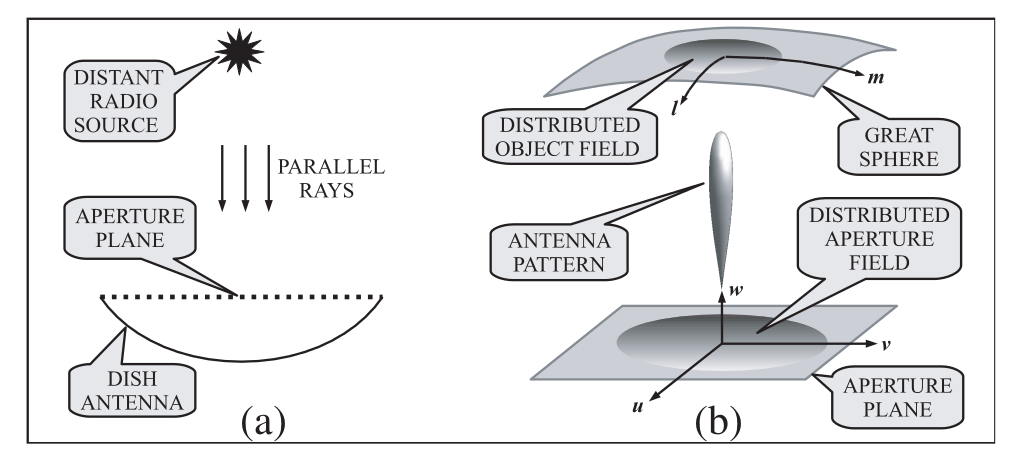
\includegraphics[width=4.2in]{c2/measure-image}
% 	    %\vspace{5 mm}	   
% 	    \caption{(a) \textit{A distant radio astronomical source illuminates a dish antenna with parallel rays.}
% 	    (b) \textit{Electric field distributions of a source on the great sphere and antenna aperture on the aperture plane}}
% 	    \label{fig:hg10}
%        \end{figure}
%   \FloatBarrier 
%   %
%   \noindent  Although single dish radio telescopes, such as the $100$ m GBT and the huge but fixed $305$ m Arecibo Observatory are very advantageous
%     in making primary surveys of the sky at low resolution, the resolution of a telescope is limited by its collecting area  \citep{wright2004single,2002Emerson}.
%     Interferometry is a technique for connecting multiple radio antennas to efficiently form single antenna with a far greater collecting area than the individual components.
%     The separation between the antennas and the rotation of the Earth leads to differences in the observed path length from the object under observation.
%     When the data from each of the antennas is put together, an interference pattern is generated, which can be reconstructed to form an image of the observation.
%     %     However, its data can be put together with antenna array also known as interferometer to obtain a good balance between lower and higher spatial frequency components.\\    
%  Instead of a single dish antenna, an interferometer with the assistance of the rotation of Earth can synthesise a large antenna aperture. This technique is known as 
%  \textit{super-synthesis} \citep{1952Machin,1974Thompson}.
%  
%  Consider a large number of radio telescopes distributed across a plane area situated at a given longitude, latitude and altitude as shown in Fig.~\ref{fig:hg11}(a), 
%  such that they track a distant radio source located on the celestial North pole. Consider also a rectangular coordinate system $(u',v',w')$ whose origin is
%  at the phase centre of telescope plane as in Fig.~\ref{fig:hg11}(b), reproduced from \citep{2010Joardar}, such that $w'$ axis points towards the zenith (source) 
%  and the $u',v'$ plane remains stationary to the observed source. From the observed source towards the antennas, due to the rotation of the Earth, 
%  the position of the antennas appears to be moving over the  $u',v'$ plane.  The outputs of individual radio telescopes is recorded at each integration time and then placed on the $u',v'$ plane.
% %
% %	+++++++++++++++++++++++++++++++++++++++++++
% %	Aperture synthesis
% %	++++++++++++++++++++++++++++++++++++++++++++
% %
% \begin{figure}[ht]
% 	    \centering	    
% 	    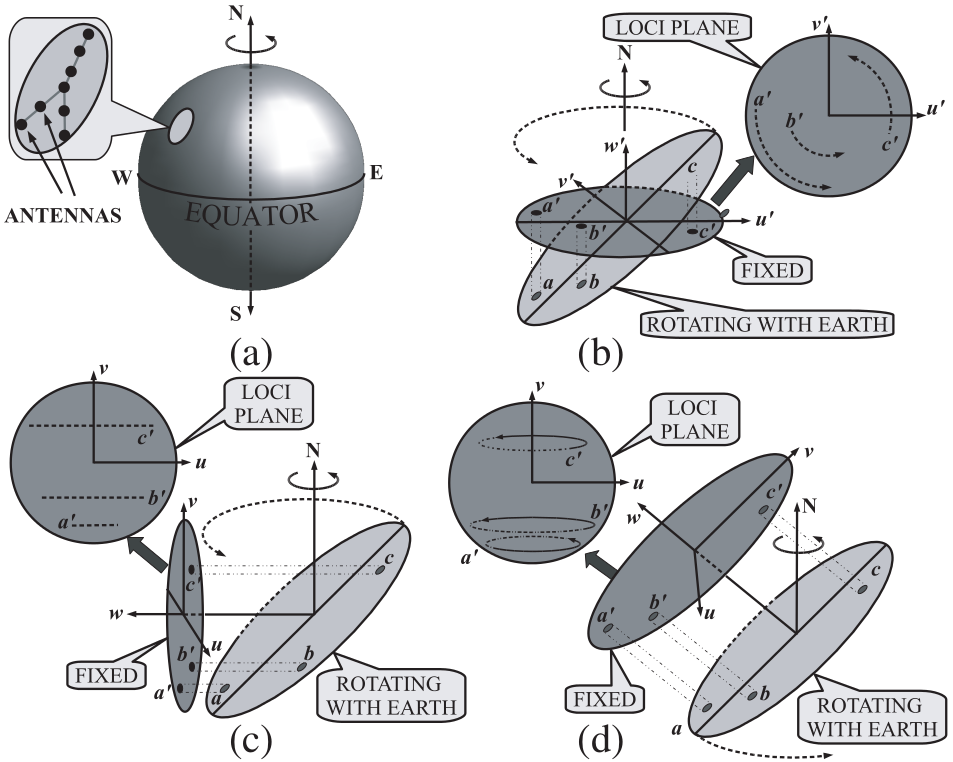
\includegraphics[width=4.2in]{c2/super-synthesis}
% 	    %\vspace{5 mm}	   
% 	    \caption{\textit{The principle of super synthesis}. (a) \textit{An interferometer rotates with the Earth rotation}
% 	    (b) \textit{Observing a radio source towards celestial North Pole.} 
% 	    (c) \textit{Observing a radio source along the celestial equator.}
% 	    (d) \textit{Observing a radio source along a celestial latitude in between.}}
% 	    \label{fig:hg11}
%        \end{figure}
%   \FloatBarrier 
%   %
%  The loci $a' , b'$ and $c'$ of the radio telescopes $a, b$ and $c$ respectively on the $u',v'$ plane forms circles over a period of 24 h.  Having numerous radio telescopes at 
%  different baselines from the origin of the $(u' , v' , w')$ coordinates over a period of 24 h,  the $u',v'$ plane gets highly populated. The $u ',v'$ plane then forms the
%  aperture of a large synthesised antenna. Thus, we apply Fourier transform on the $u',v'$ plane data after calibration to obtain the field distribution of the source.
% %
% Considering a radio source on the celestial equator as presented in Fig.~\ref{fig:hg11}(c), the loci $a',b'$ and $c'$ on the $u',v'$ plane form straight lines. Thus,
% if all the radio telescopes are mounted on a single East-West line then their respective  loci be a  straight line and this not good enough for making a radio image. It is therefore
% necessary to mount some of the radio telescopes spread along the North-South axis. If the observed source is located at a celestial latitude between $(0^{\circ}, 90^ {\circ})$ or 
% $(-90^{\circ}, 0^ {\circ})$, each of the loci form an ellipse as shown in  Fig.~\ref{fig:hg11}(d).
% %
% %
% \subsection{Correlator Super-Synthesis Arrays}	  	 \label{chap2:sec5.2}
% %
% The correlation products between any pair of antennas are used to fill the $u,v$ plane, where the $(u, v, w)$ coordinates are measured in wavelengths. If there are $N$ antennas 
% in an array, then the number of cross correlation is defined as $N\left(\frac{N-1}{2}\right)$. In any pair of antennas in an interferometer, when we fix one of the antennas 
% at the origin of the $(u, v, w)$, the baseline between the two antennas on the $u,v$ plane will rotate through $180^\circ$ in 12 h. We obtain similar observation results when the 
% other antenna is considered as the origin of the $(u, v, w)$ coordinates. This makes it possible to cover $360^\circ$ of baseline rotation in half a day. Thus, 
% data obtained from an interferometer is a measure of the spatial coherence function called \textit{visibility} and is denoted as $V(u, v)$. This visibility data covers only $1/2$
% of the $u,v$ plane from a 12 h observation, but the other $1/2$ can be obtained using Equation~\ref{eq:q26}, where $V^{*}(u, v)$ is the complex conjugate of
% $V(u, v)$. Hence, we can derive 24 h of observed data from a 12 h observation.
% %% Q26
% \begin{equation}
%   \begin{aligned}
%   V(-u, -v) = V^{*}(u, v)
%    \end{aligned}
%    \phantom{\hspace{1cm}}
%   \label{eq:q26}
%  \end{equation} 
%  %
%  %
%  
% % -------------------------------------------------------------------------------------------------------------------------------------
% 
% \subsection{The Van Cittert-Zernike equation}	  	\label{chap2:sec5.3}
% %
% Consider a two-element interferometer observing a radio source as in  Fig.~\ref{fig:hg12}(a) \citep{2010Joardar} such that the first element is positioned at the origin of the $(u, v, w)$
% coordinate system. In addition, consider $I(\gamma_1,  \gamma_2)$ to be the intensity distribution of the source on the celestial sphere such that the origin of the $l, m$
% coordinate system is at the phase reference position. If we denote $I(\bar{s})$ as the sky brightness at a frequency $\nu$ in the direction $\bar{s}$ and assume 
% $A(\bar{s})$ to be the effective aperture area of an antenna in the same direction, then the signal power received over a bandwidth $\Delta \nu$ within
% a solid angular element $d\Omega$ for each antenna is given by $A(\bar{s}) I(\bar{s}) \Delta \nu d\Omega \cos (2\pi \nu \tau_g)$. Therefore, the  correlated signal power $dr$ over
% $d\Omega$ is given as:
% %% Q27
% \begin{equation}
%   \begin{aligned}
%   dr = A(\bar{s}) I(\bar{s}) \Delta \nu d\Omega \cos (2\pi \nu \tau_g)
%    \end{aligned}
%    \phantom{\hspace{1cm}}
%   \label{eq:q27}
%  \end{equation} 
%  %
%  Integrating Equation~\ref{eq:q27} over the celestial sphere we get the correlator power $r$:
%  %% Q28
% \begin{equation}
%   \begin{aligned}
%   r(\overrightarrow{d}_{\lambda}, \bar{s}) = \Delta \nu \int A(\bar{s}) I(\bar{s}) \cos [2\pi (\overrightarrow{d}_{\lambda} \bar{s})] d\Omega 
%    \end{aligned}
%    \phantom{\hspace{1cm}}
%   \label{eq:q28}
%  \end{equation} 
%  %
%  where $\overrightarrow{d}_{\lambda}$ is the baseline  vector specified by the $(u,v,w)$ coordinates and measured in wavelengths.
% %
% %	+++++++++++++++++++++++++++++++++++++++++++
% %	interferometer synthesis
% %	++++++++++++++++++++++++++++++++++++++++++++
% %
% \begin{figure}[ht]
% 	    \centering	    
% 	    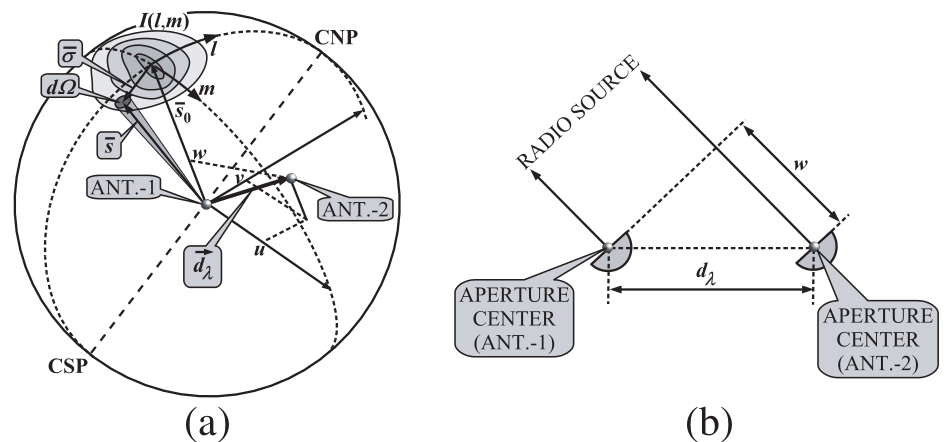
\includegraphics[width=4.8in]{c2/interferometer}
% 	    %\vspace{5 mm}	   
% 	    \caption{\textit{Geometry of a radio source and a simple interferometer}. (a) \textit{An observed radio source with intensity distribution $I(\gamma_1,  \gamma_2)$ 
% 	    using a simple two element radio interferometer.}
% 	    (b) \textit{Lower the elevation angle of the radio source the larger the value of w.} 
% 	    }
% 	    \label{fig:hg12}
%        \end{figure}
%   \FloatBarrier 
%   %
%  \noindent  If we put $ \bar{s} = \bar{\sigma} + \bar{s}_{0}$ such that $\bar{\sigma}$ is the position vector from the phase reference 
%   point to the observing point. Rewriting Equation~\ref{eq:q28} we get:
%    %% Q29
% \begin{equation}
%   \begin{aligned}
%   r(\overrightarrow{d}_{\lambda}, \bar{s}_{0}) = \Delta \nu  \cos [2\pi (\overrightarrow{d}_{\lambda} \bar{s}_{0})]  \int A(\bar{\sigma}) I(\bar{\sigma}) \cos [2\pi (\overrightarrow{d}_{\lambda} \bar{\sigma})] d\Omega\\
% 					-  \Delta \nu  \sin [2\pi (\overrightarrow{d}_{\lambda} \bar{s}_{0})]  \int A(\bar{\sigma}) I(\bar{\sigma}) \sin [2\pi (\overrightarrow{d}_{\lambda} \bar{\sigma})] d\Omega 
%    \end{aligned}
%    \phantom{\hspace{1cm}}
%   \label{eq:q29}
%  \end{equation}  
%  %
%  The visibility $V$ is defined as a complex function:
%   %% Q30
% \begin{equation}
%   \begin{aligned}
%   V = |V| \exp(j\phi_\nu) =  \int A'(\bar{\sigma}) I(\bar{\sigma}) \exp (-j2\pi \overrightarrow{d}_{\lambda} \bar{\sigma}) d\Omega 
%    \end{aligned}
%    \phantom{\hspace{1cm}}
%   \label{eq:q30}
%  \end{equation} 
%  %
%  with the real part being:
%  
%  %% Q31
% \begin{equation}
%   \begin{aligned}
%   V = |V| \cos(\phi_\nu) =  \int A'(\bar{\sigma}) I(\bar{\sigma}) \cos (2\pi \overrightarrow{d}_{\lambda} \bar{\sigma}) d\Omega 
%    \end{aligned}
%    \phantom{\hspace{1cm}}
%   \label{eq:q31}
%  \end{equation} 
%  
%  
%  \noindent and the imaginary part being:
%  
%  %% Q32
% \begin{equation}
%   \begin{aligned}
%   V = |V| \sin(\phi_\nu) =  -\int A'(\bar{\sigma}) I(\bar{\sigma}) \sin (2\pi \overrightarrow{d}_{\lambda} \bar{\sigma}) d\Omega 
%    \end{aligned}
%    \phantom{\hspace{1cm}}
%   \label{eq:q32}
%  \end{equation} 
%  %
% where, $A'(\bar{\sigma}) = \frac{A(\bar{\sigma})}{A_0}$ is the normalised beam pattern of an antenna with $A_0$ being the peak antenna gain.
% Substituting Equation~\ref{eq:q31} into~\ref{eq:q30}, we get:
%  
%   %% Q33
% \begin{equation}
%   \begin{aligned}
%   r(\overrightarrow{d}_{\lambda}, \bar{s}_{0}) = A_{0} \Delta \nu  |V| \cos [2\pi (\overrightarrow{d}_{\lambda} \bar{\sigma} - \phi_\nu)]
%    \end{aligned}
%    \phantom{\hspace{1cm}}
%   \label{eq:q33}
%  \end{equation} 
%  %
%  Equation~\ref{eq:q33} shows that an interferometer measures the visibility which is a measure of the wavefront's spatial coherence across the baseline. 
%  To produce an image from Equation~\ref{eq:q33}, we need to know their positions on the $u, v, w$ coordinate system and compare them with $l, m$ 
%  coordinate system. As the elevation angle of the observed source decreases as in Fig.~\ref{fig:hg12}(b), the $w$ term increases: 
% %% Q34
% \begin{equation}
%   \begin{aligned}
%   \overrightarrow{d}_{\lambda} \bar{s}  = ul + vm + wn
%    \end{aligned}
%    \phantom{\hspace{1cm}}
%   \label{eq:q34}
%  \end{equation} 
%  %
% If $\bar{s} = \bar{s}_{0}$ Equation~\ref{eq:q34} simplifies to:
% %% Q35
% \begin{equation}
%   \begin{aligned}
%   \overrightarrow{d}_{\lambda} \bar{s}  = w
%    \end{aligned}
%    \phantom{\hspace{1cm}}
%   \label{eq:q35}
%  \end{equation} 
%  %
% The solid angle $d\Omega $ can be expressed in polar coordinates as $d\Omega  = \sin \theta\,  d\theta d\phi$, where $\theta$ and $\phi$ are the polar and 
% azimuthal angles in the $(u, v , w)$ plane,that is, $\theta = \sin^{-1} (\sqrt{l^2 + m^2})$ and $\phi = tan^{-1} (m/l)$. Using the Jacobian method, we can transform the 
% coordinates $(\theta, \phi)$ into  $(\gamma_1,  \gamma_2)$:
% %% Q36
% \begin{equation}
%   \begin{aligned}
%   d\Omega = \frac{d\gamma_1 d \gamma_2}{n} = \frac{d\gamma_1 d \gamma_2}{\sqrt{1 - l^2 - m^2}}
%    \end{aligned}
%    \phantom{\hspace{1cm}}
%   \label{eq:q36}
%  \end{equation} 
%  %
% 
% \noindent Using Equations~\ref{eq:q34} to~\ref{eq:q36}, we can therefore rewrite the visibility $V$ in Equation~\ref{eq:q34} in terms of $u, v , w$:
% %% Q37
% \begin{equation}
%   \begin{aligned}
%   V(u,v,w) =  \int\limits_{-\infty}^{\infty} \int\limits_{-\infty}^{\infty} \, \frac{A'(\gamma_1,  \gamma_2) I(\gamma_1,  \gamma_2)}{\sqrt{1 - l^2 - m^2}} \exp \{
%   -j2\pi[ul + vm + w(\sqrt{1 - l^2 - m^2} -1)]\} dl dm
%    \end{aligned}
%    \phantom{\hspace{1cm}}
%   \label{eq:q37}
%  \end{equation} 
%  %
% 
% \noindent Equation~\ref{eq:q37} is known as \textit{van Cittert-Zernike equation} \citep{bkk13,1974Thompson,2009Rau} and it shows that the visibility $V(u, v, w)$, 
% is a Fourier transform of the product of the sky brightness $I(\gamma_1,  \gamma_2)$, the primary beam response $A'(\gamma_1,  \gamma_2)$ and $1/\sqrt{1 - l^2 - m^2}$. 
% When the distance of the observed source becomes less, $|l|$ and $|m|$ become much less such that $w(\sqrt{1 - l^2 - m^2} -1)$ approaches zero and Equation~\ref{eq:q37} reduces to:
% 
% %% Q38
% \begin{equation}
%   \begin{aligned}
%   V(u,v,w) \simeq V(u,v,0) =  \int\limits_{-\infty}^{\infty} \int\limits_{-\infty}^{\infty} \, \frac{A'(\gamma_1,  \gamma_2) I(\gamma_1,  \gamma_2)}{\sqrt{1 - l^2 - m^2}} \exp \{-j2\pi(u\gamma_1 + v\gamma_2)\} dl dm
%    \end{aligned}
%    \phantom{\hspace{1cm}}
%   \label{eq:q38}
%  \end{equation} 
%  %
% and the inverse transform being defined by:
% 
% %% Q39
% \begin{equation}
%   \begin{aligned}
%   \frac{A'(\gamma_1,  \gamma_2) I(\gamma_1,  \gamma_2)}{\sqrt{1 - l^2 - m^2}}  =  \int\limits_{-\infty}^{\infty} \int\limits_{-\infty}^{\infty} \, V(u,v)  \exp \{j2\pi(u\gamma_1 + v\gamma_2)\} du dv 
%    \end{aligned}
%    \phantom{\hspace{1cm}}
%   \label{eq:q39}
%  \end{equation} 
%  %
%  %
%  
%  % -------------------------------------------------------------------------------------------------------------------------------------
% 
% \subsection{Filling the \emph{u,v} Plane with Visibilities}	  \label{chap2:sec5.}
% %
% Consider the phase reference position of an observed radio source is at $(H_{0}, \varphi_{0})$ in the local equatorial coordinate system. Assume $X_{\lambda}, Y_{\lambda}$ and
% $Z_{\lambda}$ are the baseline components in a rectangular coordinate system measured in wavelengths \citep{bkk13}, then the $u,v$ can be written as;
% %% Q40
% \begin{equation}
%   \begin{aligned}
%   u^{2} + \left[\frac{v - Z_{\lambda}\cos(\varphi_{0})}{\sin (\varphi_{0})}\right]^{2} = X_{\lambda}^{2} + Y_{\lambda}^{2}
%    \end{aligned}
%    \phantom{\hspace{1cm}}
%   \label{eq:q40}
%  \end{equation} 
%  %
%  Equation~\ref{eq:q40} represents an ellipse which splits into $2$ in the $u, v$ plane if $Z_{\lambda} \neq 0$  \citep{bkk13}. Fig.~\ref{fig:hg13}(a) produced from \citep{2010Joardar}
%  displays Equation~\ref{eq:q40} when observing a radio source at declination $\varphi_{0})$. That for Fig.~\ref{fig:hg13}(b) displays cases of a North-South baseline for 
%  different values of $\varphi_{0}$.
% %	+++++++++++++++++++++++++++++++++++++++++++
% %	declination plot
% %	++++++++++++++++++++++++++++++++++++++++++++
% %
% \begin{figure}[ht]
% 	    \centering	    
% 	    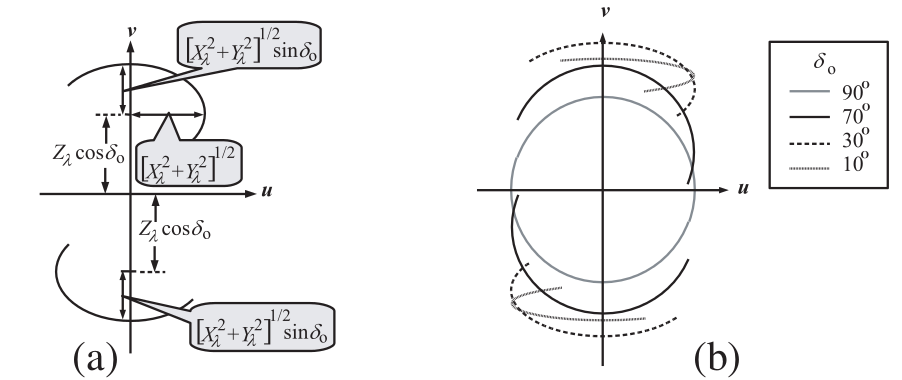
\includegraphics[width=4.8in]{c2/uv-plane}
% 	    %\vspace{5 mm}	   
% 	    \caption{\textit{Locus on the $u, v$ plane.}. (a) \textit{Locus of the
% ellipse on $u, v$ plane for a baseline with $Z_{\lambda} \neq 0$ observing a radio source at declination $\varphi_{0}$.}
% 	    (b) \textit{Different declinations for different cases.} 
% 	    }
% 	    \label{fig:hg13}
%        \end{figure}
%   \FloatBarrier 
%   %
% \noindent The KAT-7 consists of seven observing antennas located at latitude $-30^{\circ}$, longitude $21^{\circ}$ and altitude $1038 \,\mathrm{m}$ in configuration as shown in Fig.~\ref{fig:hg14}(a).
% Fig.~\ref{fig:hg14}(b) displays the $u,v$ coverage at particular synthesis time with observed radio source at the phase centre. The circular structure rotates along with the Earth.
% If the zenith coincides with a celestial pole, then each point traces out a circle. Otherwise, the tracings could be elliptical, broken ellipse, or straight line (zero declination).
% When we increase the synthesis time, more data fill the \emph{uv} plane. Using Equation~\ref{eq:q39}, the intensity distribution $I(\gamma_1,  \gamma_2)$ or image of the radio source is made. This is 
% actually done after calibrating the data \cite{bkk13,1974Thompson,2009Rau,2016arXiv160302126B,2016A&A...586A..76J}.
%  %
%  \begin{figure}[ht]
%   \centering
%      \begin{subfigure}[b]{0.49\textwidth}
%                 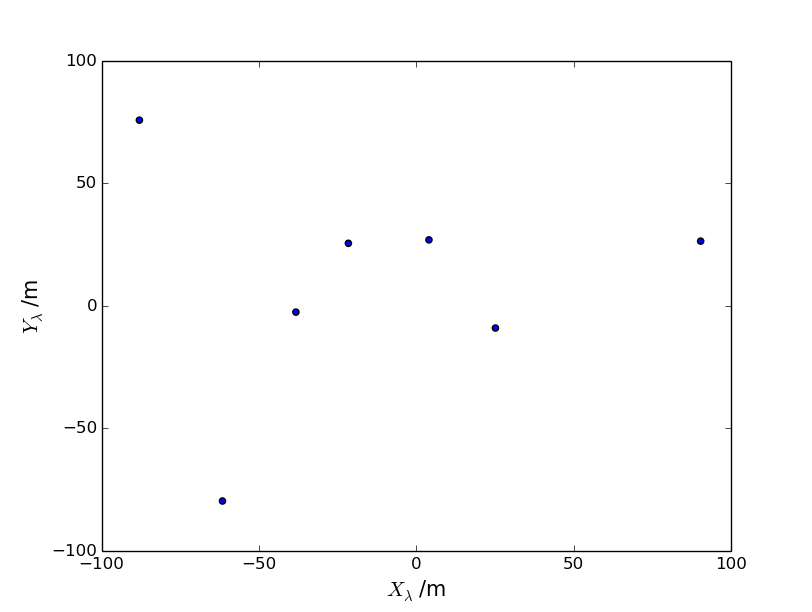
\includegraphics[width=\textwidth]{c2/kat7-setup}
%                 \caption{}
%                 %\label{fig:lab0}
%         \end{subfigure}       
%         \begin{subfigure}[b]{0.50\textwidth}
%                 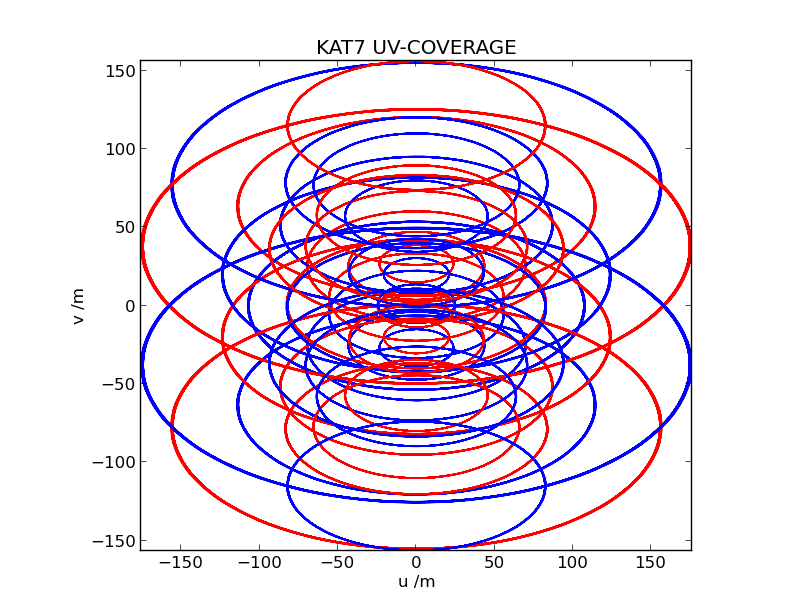
\includegraphics[width=\textwidth]{c2/msuv}
%                 \caption{}
%                % \label{fig:lab1}
%         \end{subfigure}
%         \caption{\textit{Filling the u-v plane with visibilities}. (a) \textit{The KAT-7 configuration.}
% 	    (b) \textit{The u-v plane coverage of a $4 \,\mathrm{h}$ period of observation obtained from a source at the phase centre.} 
% 	    }
% 	    \label{fig:hg14}
%   \end{figure}
% \FloatBarrier 
% %
% 
% \noindent Using the Fast Fourier Transform (FFT) approach, the data on \emph{u,v} plane is interpolated on a uniform grid \citep{bkk13,2005Fu,2007Zhang} and 
% at the same time employs the tapering technique \citep{bkk13} to reduce the side lobes of the synthesised antenna beam. The dirty image obtained after FFT may contain lots of 
% artefacts \citep{2016arXiv160107182D}. These are removed using algorithms such as  CLEAN \citep{2009GGG....10.9U07A,1998Camps,2010ISPM...27...14L,2012JPhCS.355a2020C} or
% MEM \citep{2012JPhCS.355a2020C,2016A&A...586A..76J,2013arXiv1307.6757C}. 







% %	+++++++++++++++++++++++++++++++++++++++++++
% %	kat7 image plot
% %	++++++++++++++++++++++++++++++++++++++++++++
% %
% \begin{figure}[ht]
% 	    \centering	    
% 	    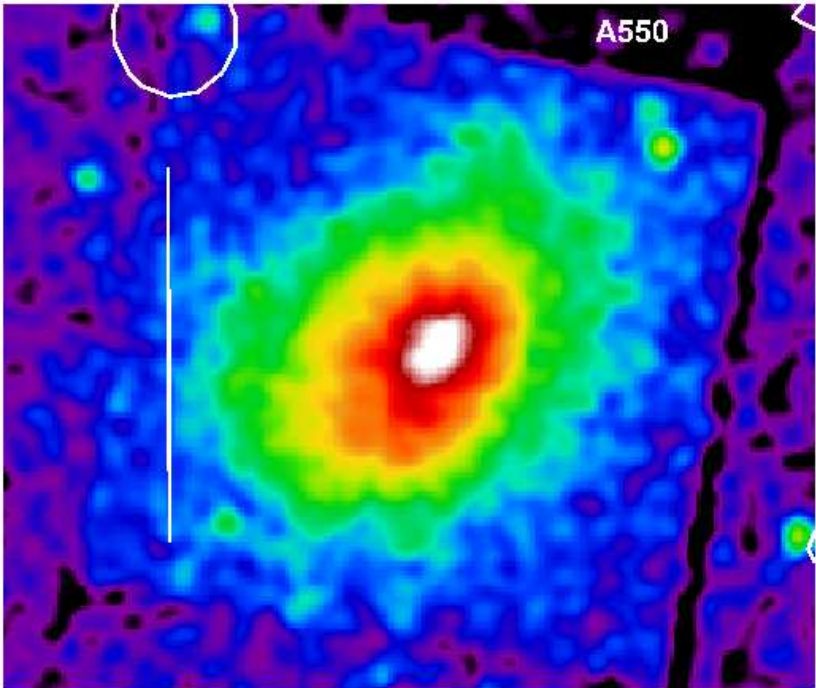
\includegraphics[width=4.8in]{c2/GB}
% 	    %\vspace{5 mm}	   
% 	    \caption{\textit{: 1.86 GHz KAT–7 radio contours of the A 550 cluster overlaid on the X–ray XMM–Newton images as an example of target that does
% 	    not show any diffuse radio emission corresponding to the cluster centre. 
% 	    The image is not corrected by the primary beam. The vertical white bar indicates a $800 kpc$ size.}. 
% 	    }
% 	    \label{fig:hg15}
%        \end{figure}
%   \FloatBarrier 
%   %
% Fig.~\ref{fig:hg15} displays $1.86$ GHz KAT–7 radio contours of the A 550 cluster as in \citep{2016arXiv160307595B} and drawn at $-2.5, 2.5, 10$ and $40 \, mJy\, beam^{-1}$
% with positive (negative) contours drawn using solid (dashed) lines. 
% 
% 
% 
% 

















 

\chapter{Radio Foregrounds and Rotation Measure Synthesis} % Main chapter title

\label{Chapter3} % For referencing the chapter elsewhere, use \ref{Chapter1} 

\textbf{Overview}\\
% \HRule \\[0.4cm]
\par\noindent\rule{\textwidth}{0.4pt}\\
\textit{This chapter presents a brief theoretical review of the diffuse synchrotron emis-
sion and Faraday rotation. We then discuss the simulation algorithm used to
produce the foreground maps with rotation in this research.}
\par\noindent\rule{\textwidth}{0.4pt}\\
% --------------------------------------------------------------------------------------------------------------------------------

%\lhead{Chapter 3. \emph{Cosmological Signal}}


% \HRule \\[1.5cm]
% --------------------------------------------------------------------------------------------------------------------------------
\noindent \texttt{Author’s comment}: 
%%
\small{Part of this work is taken from: \textbf{T. Ansah-Narh}, F. B. Abdalla, O. M. Smirnov, K. M. B. Asad and J. R. Shaw, (2018). Simulations of Systematic Direction-dependent Instrumental Effects in Intensity Mapping Experiments. Monthly Notices of the Royal Astronomical Society (MNRAS), published. It is therefore, widely recognized that some of the text and figures will match that of the article. Therefore, this comment serves as a general reference for all such text.
}

\section{Galactic Foreground}	   \label{chap3:sec1}
%% 
% \texttt{Author’s comment: The indentation part in this section is taken from the work of} \citep{ansah2018simulations}.
% A varying magnetic field can accelerate charge particles to emit radiation.
The measurements of redshifted CO and 21 cm emissions are very powerful tools to understand the star formation and survey the structure of the Universe respectively. 
The emission emerging from different astrophysical sources, other than the signals mentioned above, results in the foreground emission whose magnitude can be the higher than
fourth order of the expected signals. The EM emission from particles normally electrons accelerated by the death of a star and supernova remnant, in the presence of a magnetic field, 
is called the \emph{synchrotron emission}. The synchrotron emission from the Galaxy dominates at low microwave frequencies $(\lesssim 30 \, \rm GHz)$, 
whilst that of thermal dust emission is at higher frequencies $(\gtrsim 70 \, \rm GHz)$. Between these two components in frequency, lies the thermal free-free and non-thermal 
dust emissions, which are formed as a result of spinning dust grains \citep{2016A&A...594A..10P} as shown in Fig.~\ref{fig:cmb1}. 
The free-free emission (also known as thermal bremsstrahlung) is obtained from thermally hot electrons ($\gtrsim 10^4\, \rm K$) \citep{1999astro.ph..2201S} scattering uniformly in
the interstellar plasma hence, having a completely zero polarisation. In the case of the thermal dust emission,
it is formed from dust grains that get warmed by the interstellar radiation field and then emit far-infrared light which eventually lead to multiple temperatures.
The dust grains are composed of Polycyclic Aromatic Hydrocarbons (PAHs), silicates, and graphites. 


%	+++++++++++++++++++++++++++++++++++++++++++
%	Foreground Emission
%	++++++++++++++++++++++++++++++++++++++++++++
%
\begin{figure}[ht]
	    \centering	    
	    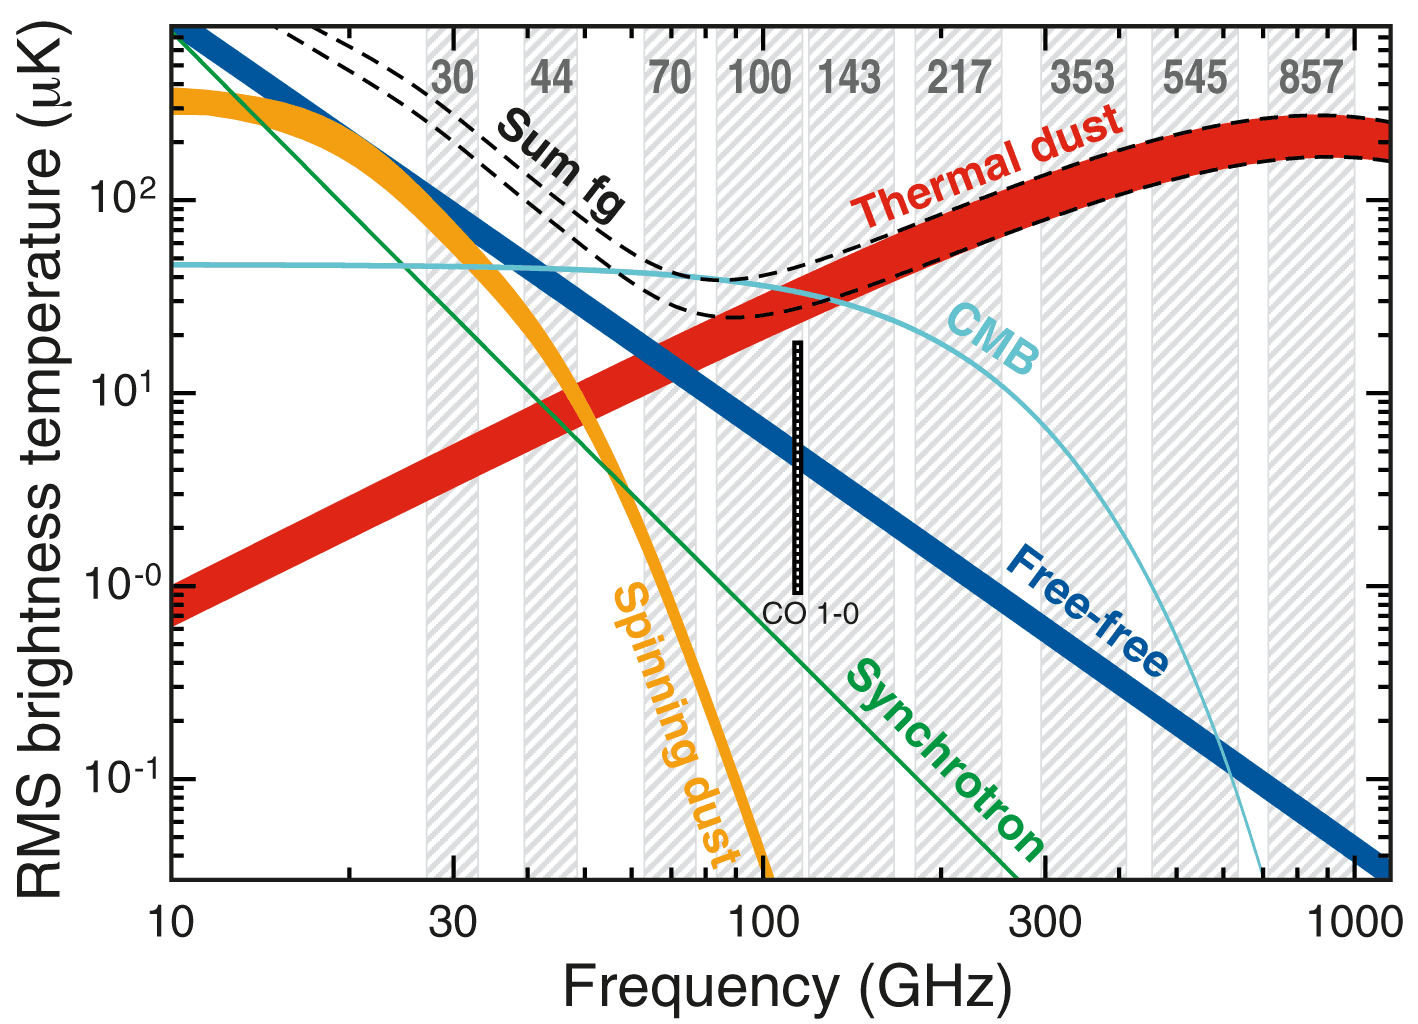
\includegraphics[width=3.8in]{c3/Planck_A12_Fig24_left} %cmb1}	    	   
	    \caption{\theo{Brightness temperature distribution for the components of the Galactic foregrounds with respect to frequency. 
	    The angular resolution for the temperature of each smooth component is $1^\circ$.
	    \emph{Credit:} This figure is obtained from \citep{2016A&A...594A..10P}.}} \label{fig:cmb1}
% 	    {\textit{A model of radio galaxy spectrum \citep[see][]{Murphy:2010kk}. The individual contributions from non-thermal synchrotron, 
% 	    free-free, and thermal dust emission are indicated by dot-dashed, triple dot-dashed, and dashed lines, respectively.} }	   
       \end{figure}
  \FloatBarrier  

\noindent Detailed discussion of the components of the Galactic foregrounds, paying particular attention to their contributions to the polarization
measurements can be found in \cite{2015MNRAS.447..400A,2010MNRAS.409.1647J,2015aska.confE..19S,2014MNRAS.441.3271W}.
% }
% \citep{ansah2018simulations}
% \end{quotation}
 %%
%%


%
\subsection{Diffuse Galactic Synchrotron Emission}	   \label{chap3:sec2.1}
%

 
% A varying magnetic field can accelerate charge particles to emit radiation.
% Galactic synchrotron radiation occurs when the interstellar  magnetic field interacts with charged particles (electrons and positrons) in the cosmic-ray.
% These interacting particles are accelerated to relativistic speeds in very high energetic environments,
% such as shock-waves from supernovae explosions. The synchrotron intensity and spectrum depend on the magnetic field strength and cosmic ray energy,
% showing significant spatial variations on the sky. The energy distribution of cosmic ray electrons follows a power-law 
\theo{
In Section~\ref{chap3:sec1}, we emphasized that the intensity of the synchrotron radiation relies on the strength of the magnetic field and the cosmic-ray energy. 
The distribution of this energy can be given as a function of a power law (also known as scaling law) such that $N_{\rm \,E} \varpropto E^{-\tau}$, where 
$E > 10$ GeV is the energy \citep{2011PhRvL.106t1101A} and $\tau \approx 3.0 $ is the spectral index  of the energy distribution (this index value is usually accepted when modelling
in synchrotron and magnetic field). }
%%

\theo{The intensity of a synchrotron radiation $S_{\rm \, sync}$ with a frequency $\nu$ is defined as \citep{MD2008}: 
% %
\begin{equation}  \label{eq:th1}
  S_{\rm \,  sync}(\nu) = \varepsilon_{\rm \, sync}(\nu)\, \int\limits_z \, n_{\rm \, e}B_{\rm \, \perp}^{(1+\tau)/2}\, dz   
 \end{equation} 
% 
}
\theo{where Equation~\ref{eq:th1} is integrated with respect to the sight-line $z$, $n_{\rm \, e}$ is cosmic ray density and 
$B_{\rm \, \perp} = \sqrt{B_{\rm \, x}^{2} + B_{\rm \, y}^{2}}$ is the $x,y$  components of the magnetic field of the sky.
From the power law, we can express the emissivity term $ \varepsilon_{\rm \, sync}(\nu)$ as:
 %
\begin{equation}
 \varepsilon_{\rm \, sync}(\nu) = \varepsilon_{\rm \, 0}\, \nu^{-(\tau - 1)/2}
 \label{eq:th2}
 \end{equation} 
 %
}
\theo{Recall Rayleigh-Jeans law at frequency $\nu$:
 %
\begin{equation}
  B_{\rm \, \nu}(T) = \frac{2\nu^{2}k_{\rm \, B}T}{c^2}
  \label{eq:th3}
 \end{equation} 
 %
 where $c$ denotes the speed of light, $k_{\rm \, B}$ being the Boltzmann constant and $T$ is the temperature in Kelvin. Using Equation~\ref{eq:th3}, 
 we can convert Equation~\ref{eq:th1} into a brightness temperature $T_{\rm \, sync}$ at frequency $\nu$:
 %
\begin{equation}
  T_{\rm \, sync}(\nu) = \frac{c^{2}S_{\rm \, sync}(\nu)}{2k_{\rm \, B}\nu^2}
  \label{eq:th4}
 \end{equation} 
 %
} 
 \theo{Hence, expressing $T_{\rm \, sync}$ as a power law, we get:
 %
\begin{equation}
  T_{\rm \, sync}(\nu) = T_{\rm \, sync}(\nu_0)\left(\frac{\nu}{\nu_0}\right)^{\gamma_{\rm \, sync}}
  \label{eq:th5}
 \end{equation} 
 %
 where $\gamma_{\rm \, sync} = -(\tau + 3)/2$. The spectral index $\gamma_{\rm \, sync}$, changes at  different frequency bands as displayed in Table~\ref{table:2}.}
 %
%

\begin{table}[H]
\caption{Measured Spectral Indices at Different Frequency Bands}             % title of Table
\label{table:2}      % is used to refer this table in the text
%\begin{threeparttable}
\centering                          % used for centering table
\begin{tabular}{c c}        	  % centered columns (4 columns)
\hline\hline                	  % inserts double horizontal lines
\textbf{$\gamma_{\rm \, sync}$} & \textbf{Frequency Band ($\rm GHz$)}\\    % table heading 
   %
\hline                        % inserts single horizontal line
  $-2.55$ & $0.045 - 0.408$ \\      % inserting body of the table
  $-2.71$ & $0.408 - 2.30$ \\
  $-3.01$ & $2.300 - 33.0$ \\  
\hline                                   %inserts single line
\end{tabular}
% 
\end{table}
 \FloatBarrier 
\theo{
\noindent Fig.~\ref{fig:ch3.3} is the $408$ MHz full-sky survey taken from the LAMBDA-Data Products\footnote{ 
\url{https://lambda.gsfc.nasa.gov/product/foreground/fg_2014_haslam_408_info.cfm}} \citep{2015MNRAS.451.4311R} and originally produced by \citep{1981A&A...100..209H,HaslamMap} 
displaying the sky in mollview form in Galactic  coordinates at a frequency where the diffuse synchrotron emission is most dominant. We can clearly observe other sources 
 outside the Milky Way such as Cen A galaxy and the Magellanic clouds. An in-depth explanation on the concept of synchrotron emission is conferred in \citep{lightman1979radiative}.
}
 %
%	+++++++++++++++++++++++++++++++++++++++++++
%	full-sky map
%	++++++++++++++++++++++++++++++++++++++++++++
%
\begin{figure}[ht]
	    \centering	    
	    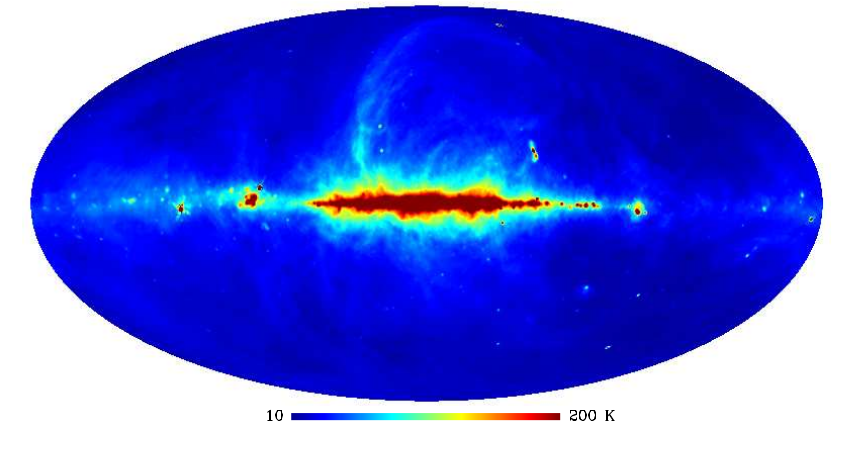
\includegraphics[width=3.8in]{c3/haslam}	    	   
	    \caption{$408$ MHz Full-Sky Map \citep{1981A&A...100..209H} projected in HEALPix, ring
and defined in Galactic coordinates. Data and images can be retrieved from the LAMBDA website.}
	    \label{fig:ch3.3}
       \end{figure}
  \FloatBarrier   
  %
\theo{
\noindent However, studies such as \citep{2010MNRAS.409.1647J,2018ApJ...855...29H} have shown that generally, the diffuse Galactic synchrotron emission is incompletely 
linearly polarised. This is due to the \enquote{spatial and energy distribution of the cosmic ray electrons, as well as the strength and orientation of 
the perpendicular (with respect to the line of sight) component of the Galactic
magnetic field} \citep{2010MNRAS.409.1647J}. Note that the distribution of charge particles can alter smoothly with  pitch angle and this can eliminate the circular part and hence, 
become partially linearly polarised. Therefore, using the cosmic rays and magnetic field distributions of a galaxy, we can predict 
the polarisation foreground from the synchrotron emission and then separate it from observed maps.
The degree of linear polarisation integrated over all electron energy and frequency 
is computed as $l = (\tau + 1)/(\tau + 7/3)$\citep{2010MNRAS.409.1647J,lightman1979radiative}. The polarisation factor ($l$) can be increased to $0.75$ if 
the cosmic ray spectral index $\tau \approx 3$. We can express the polarised intensity in terms of Stokes parameters $Q$ and $U$ at frequency $\nu$ such that:
}
%
\theo{
\begin{equation}
  \begin{aligned}
  lI_{\rm \nu} = \sqrt{Q_{\rm \nu}^2 + U_{\rm \nu}^2}
   \end{aligned}
%    \phantom{\hspace{1cm}}
  \label{eq:th6}
 \end{equation} 
 %%
\noindent with the angle of polarisation given as:
%
%
\begin{equation}
  \begin{aligned}
  \varphi_{\rm \nu} = \frac{1}{2}\arctan \left( \frac{U_{\rm \nu}}{Q_{\rm \nu}} \right)
   \end{aligned}
%    \phantom{\hspace{1cm}}
  \label{eq:th7}
 \end{equation} 
 %
Therefore, in the $Q,\, U$ plane, the modulus of the complex linear polarisation is computed as ($\lvert Q_{\rm \nu} + jU_{\rm \nu} \rvert$).
From Equation~\ref{eq:th1}, we can integrate the polarised parameters ($Q$ and $U$) along the sight-line $z$ as \citep{MD2008}:
%
%
 %
\begin{equation}
  \begin{aligned}
  Q_{\rm \, sync}(\nu) = l_{\rm \, sync}\varepsilon_{\rm \, sync}(\nu)\, \int\limits_z \, n_{\rm \, e}B_{\rm \, \perp}^{(1+\tau)/2} \cos(2\alpha)\sin(\beta)\, dz
  \end{aligned}
%    \phantom{\hspace{1cm}}
  \label{eq:th8}
 \end{equation} 
 % 
%
and 
%
%
 %
\begin{equation}
  \begin{aligned}
  U_{\rm \, sync}(\nu) = l_{\rm \, sync}\varepsilon_{\rm \, sync}(\nu)\, \int\limits_z \, n_{\rm \, e}B_{\rm \, \perp}^{(1+\tau)/2} \sin(2\alpha)\sin(\beta)\, dz
  \end{aligned}
%    \phantom{\hspace{1cm}}
  \label{eq:th9}
 \end{equation} 
%
\noindent where $\cos(2\alpha) = \frac{B_x^2 - B_y^2}{B_{\rm \, \perp}^2} \quad 0 < \cos(2\alpha) < 1 $,\\
$\sin(2\alpha) = -\frac{B_x^2B_y^2}{B_{\rm \, \perp}^2}  \quad 0 < \sin(2\alpha)< 1$ and 
$\sin(\beta) = \sqrt{1 -\frac{B_x^2}{B_{\rm \, \perp}^2}}  \quad 0 < \sin(\beta) < 1$.
}


\section{Faraday Rotation Measure Synthesis}	    \label{chap3:Faraday}
%%
% \emph{Polarisation} is the term used to describe the orientation of the electric field in a light wave.
Usually, light is not polarized when created but can be made so by transporting it through a medium which transmits electric fields oriented in a specific direction and absorbs all others. 
Radio emission from astronomical sources, such as galactic and extra-galactic sources and pulsars is often linearly polarized. Of course, other sources such as OH masers from galactic star formation due to Zeeman splitting 
are mostly circularly polarized \citep{2008ApJ...680..981R}. Generally, polarization in radio astronomy is related to the presence of magnetic fields. 
For instance, radio emission due to synchrotron radiation is linearly polarized with the electric vectors and it is directed at right angles to the magnetic field in the line of emission 
onto the sky plane \citep{2012A&A...540A..80B}. However, the polarization direction may alter as the radio waves
propagate through the ISM. This effect is called the Faraday rotation and it allows radio astronomers to understand the magnetic field strength in the line-of-sight for both ISM and
Earth's ionosphere.
%heiles2008zeeman

The degree of polarization of Faraday rotation is quantified in terms of it's rotation measure ($\Phi_{\rm \, RM}$) and it is mathematically expressed as;
%%
\begin{equation}\label{eq:pangle}
\chi(\lambda) = \chi_{\rm \, 0} + \Phi_{\rm \, RM}.\lambda^2 
\end{equation}

such that, 
 \begin{equation}\label{eq:rm}
  \Phi_{\rm \, RM} = 0.81 \int_{\rm \, source}^{observer} n_{\rm \, e} \vec{B}.d \vec{l}	
 \end{equation}
%\overrightarrow{B}

\noindent where the polarization angle measured at wavelength $\lambda$ is $\chi(\lambda)$, $\chi_{\rm \, 0}$ is the intrinsic polarization,
$n_{\rm \, e}$ is the density electron in cm\textsuperscript{-3}, $\mathbf{B}$ in $\mu$G describes the magnetic field  and $l$ in pc denotes the length of path.
 $\vec{B}.d \vec{l}$ describe the direction of the magnetic field along the sight line.
%%


The observed complex polarization is described by \citep{1966MNRAS.133...67B} as $P(\lambda^2) = pI\exp(2j\chi)$, where $p$ is the degree of polarization. Substituting 
Equation~\ref{eq:pangle} for $\chi$ in \citep{1966MNRAS.133...67B} equation and integrating over all possible values of the rotation measure to get;

 \begin{subequations}\label{eq:sub}
 \begin{align}
  P(\lambda^2) &=\, \int_{\rm \, - \infty}^{+ \infty} pI\exp(2j[\chi_{\rm \, 0} + \Phi_{\rm \, RM}.\lambda^2 ]) d\Phi_{\rm \, RM} \label{eq:suba}\\
               &=\, \int_{\rm \, - \infty}^{+ \infty} F(\Phi_{\rm \, RM})\exp(2j\Phi_{\rm \, RM}.\lambda^2) d\Phi_{\rm \, RM} \label{eq:subb}
  \end{align}
 \end{subequations}
%%
where the intrinsic polarized flux is characterised by the \emph{Faraday dispersion function} $F(\Phi_{\rm \, RM})$ in terms of Faraday depth.
Note how the expression in Equation~\ref{eq:subb} takes the form of a Fourier transform. Therefore, we can invert Equation~\ref{eq:subb}  to obtain the intrinsic
polarization in terms of observable quantities to have;
%%
\begin{equation}\label{eq:invert}
F(\Phi_{\rm \, RM}) = \int_{\rm \, - \infty}^{+ \infty} P(\lambda^2)\exp(-2j\Phi_{\rm \, RM}.\lambda^2) d\lambda^2
\end{equation}
%%

% \noindent  \citep{2005A&A...441.1217B} proposed a window function $W(\lambda^2)$ to address the situations where we cannot observe at wavelengths $\lambda^2 < 0 $ 
% nor observe at all values of $\lambda^2 > 0 $.
%%

In the next section, we present how to simulate the polarized sky maps used in this research and account for the Faraday rotation. 

%% 

 \section{Simulation}    \label{sec:simulation}
%%
We apply the \texttt{CORA} software package\footnote{{\url{https://github.com/radiocosmology/cora/}}} \citep{shaw2015coaxing,Shaw:2013} to reproduce the 
complete polarization sky maps at different frequencies as shown in Figs.~\ref{fig:f1000} to~\ref{fig:f1306}. Even though the foreground simulations
are produced in a scheme similar to those described in \cite{shaw2015coaxing}, we have significantly expanded the description in this work to make it more self contained. 
% 

As now described in \citep{ansah2018simulations}, the polarization sector is simulated by generating a distribution of polarized emission in Faraday space. 
This is designed to make simulations sufficiently complex in the spectral direction, roughly reproduce the polarized 
amplitude across the sky, but does not attempt to match polarization angles anywhere. In addition, the spectral structure of the polarized signal 
from the galaxy occurs because the emission is from a range of Faraday depths. 
As suggested, the 3D structure of the galaxy, particularly the magnetic field means that emission from different regions along the 
line-of-sight collect varying amounts of Faraday rotation. In general, this gives complicated frequency dependent polarized structure 
with multiple independent Faraday components \citep[see Figure 9]{wolleben2010rotation}. Accurate mapping of this distribution is difficult, 
but is being attempted by projects such as GMIMS\footnote{{Global Magneto-Ionic Medium Survey}} \citep{GMIMS}. The most useful full-sky 
polarization measurements come from $1.4$ GHz surveys \citep{Wolleben2006,Testori2008}, the WMAP $23$ GHz \citep{WMAP_9yr_maps},
and Planck $30$ GHz maps \citep{Planck_2015_maps}. However, because of the uncertain amount of instrumental depolarization in the former and the much 
higher frequencies of the latter, these are more useful to tell us about the general properties of the polarized sky (such as the high galactic latitude
polarization fraction, see \cite{Kogut2007}) and less about the specific realisation on the sky.
Due to these drawbacks, the level of polarization within the galactic plane produced in the simulations is appropriate for IM experiments.  %\\~\\
%%
\begin{figure}[ht]
	    \centering
	    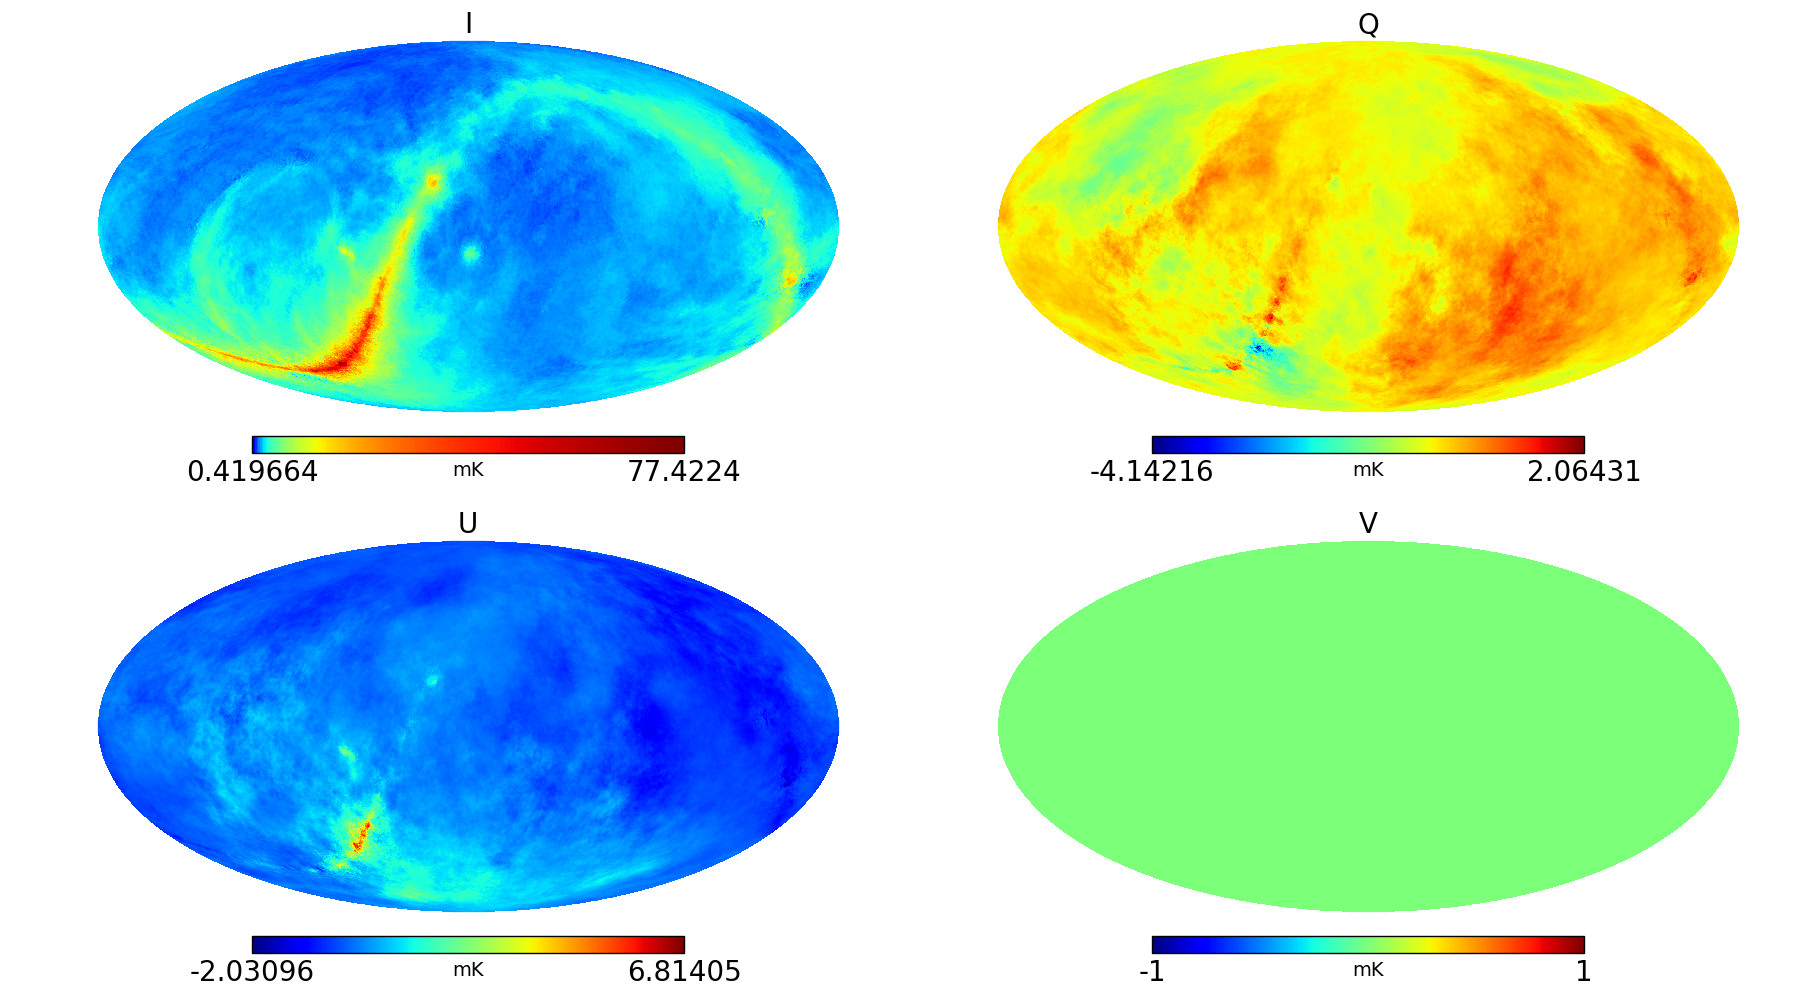
\includegraphics[width=6.0in]{c4/sec3gp_conv/Tchan_253}
	    \caption{1000 MHz full-sky simulated synchrotron maps. These synchrotron maps characterize the 
     full-sky polarization maps for our low resolution simulated observations and are presented here in the mollweide projection form defined by equatorial coordinates in terms of Stokes parameters $I, Q, U$ and $V$.}
	    \label{fig:f1000}
       \end{figure}
\FloatBarrier

Below is the scheme used to generate the foreground simulations:

\begin{enumerate}[label=(\roman*)]
 \item A 3D base map for the unpolarized sky is produced by extrapolating the $408$ MHz \cite{HaslamMap} map to the requested set of frequencies using 
    the spectral index of map of \cite{MD2008} which     was produced by comparing the Haslam map with WMAP $23$ GHz polarization data, assuming that both are dominated by 
    synchrotron emission. This produces a map with power law spectral behaviour with angular fluctuations on scales $\gtrsim 1^\circ$ scales.

    \item Angular and spectral fluctuations are added into the 3D maps according to an angular power spectrum.
    \begin{equation}
        C_\ell(\nu, \nu') \propto \biggl(\frac{\ell}{\ell_0}\biggr)^{-2.8} \biggl(\frac{\nu \nu'}{\nu_0^2}\biggr)^{-2.8} \exp{\Biggl[- \frac{1}{2} \biggl(\frac{\ln{\nu / \nu'}}{4}\biggr)^2\Biggr]} \; ,
    \end{equation}
    taken from \cite{SantosCoorayKnox}. We use a position dependent scaling on large scales to ensure the fluctuations to match their observed variance across the sky
    \citep{LaPorta2008},
    and ensure that we don't add in additional fluctuations on scales constrained by the Haslam map by projecting out the the dominant eigenmodes on these scales.

    \item To simulate the polarized sky, we use the ideas of Faraday Rotation Measure Synthesis \citep{Brentjens2005} and a simple model of the distribution of emission in 
    Faraday depth across the full sky, which we then integrate over to generate the polarized output at each desired frequency. To produce the emission in Faraday space, 
    we use the rotation 
    measure map of \cite{Oppermann2012} to indicate the characteristic scale of the distribution of emission in Faraday depth. We tune the amplitude and correlation 
    properties in Faraday 
    space to crudely reproduce the polarization fraction in the WMAP $23$ GHz map and the $1.4$ GHz surveys. The polarization directions are generated as 
    a Gaussian random field at each
    Faraday depth. For the interested reader, more details of this are found in  \cite{shaw2015coaxing}.

    \item Known bright point sources on the sky are included explicitly, with their polarizations Faraday rotated to the desired frequencies using the \cite{Oppermann2012} map. 
    Faint sources ($S < 10$ Jy at $151$ MHz) are randomly generated.
\end{enumerate} 


Finally, we use the \enquote{Hierarchical Equal Area isoLatitude Pixelation} (\texttt{HEALPix}\footnote{\url{http://healpix.sourceforge.net/}}) 
software \citep{calabretta2007mapping,2005ApJ...622..759G} to project the simulated full-sky maps
into equal pixel area, using a resolution of $N_{\rm \, \rm s} = 512$. This makes our gridded map to uniformly distribute $12N_{\rm \, \rm s}^2$ pixels onto a unit sphere. 
The regular synchrotron maps in Figs.~\ref{fig:f1000} to~\ref{fig:f1306} are depicted in  \texttt{HEALPix} format at different frequencies. 


%  
%  \begin{figure}[H]{\columnwidth}
%       \centering      
%       \includegraphics[width=\linewidth]{/c5/mkk/m/mk_fraw1}         
%      \caption{$950$ MHz full-sky synchrotron maps simulated by using m-mode formalism.}
% 	    \label{fig:fgc5}    
%     \end{figure}
\begin{figure}[ht]
	    \centering
	    \includegraphics[width=6.0in]{c5/mkk/m/mk_fraw1} 
	    \caption{Simulated foreground maps at 950 MHz displayed in mollweide form.}
	    \label{fig:f950}
       \end{figure}
\FloatBarrier
%    
%   \begin{figure}[H]{\columnwidth}
%       \centering      
%       \includegraphics[width=\linewidth]{/c6/spatial/fb1}        
%      \caption{$450$ MHz full-sky synchrotron maps simulated by using m-mode formalism.}
% 	    \label{fig:fgc6B1}    
%     \end{figure}
   \begin{figure}[ht]
	    \centering
	    \includegraphics[width=6.0in]{c6/spatial/fb1}  
	    \caption{Simulated foreground maps at 450 MHz presented in mollweide form.}
	    \label{fig:f450}
       \end{figure}
\FloatBarrier 
% \begin{figure}[H]{\columnwidth}
%       \centering      
%       \includegraphics[width=\linewidth]{/c6/spatial/fb2}         
%      \caption{$990.5$ MHz full-sky synchrotron maps simulated by using m-mode formalism.}
% 	    \label{fig:fgc6B2}    
%     \end{figure}
   \begin{figure}[ht]
	    \centering
	    \includegraphics[width=6.0in]{c6/spatial/fb2}   
	    \caption{Simulated foreground maps at 990.5 MHz displayed in mollweide form.}
	    \label{fig:f990}
       \end{figure}
\FloatBarrier   
%  \begin{figure}[H]{\columnwidth}
%       \centering      
%       \includegraphics[width=\linewidth]{/c6/spatial/fb5}         
%      \caption{$4.6$ GHz full-sky synchrotron maps simulated by using m-mode formalism.}
% 	    \label{fig:fgc6B5}    
%     \end{figure}   
  \begin{figure}[ht]
	    \centering
	    \includegraphics[width=6.0in]{c6/spatial/fb5}   
	    \caption{Simulated foreground maps at 13.6 GHz presented in mollweide form.}
	    \label{fig:f1306}
       \end{figure}
\FloatBarrier    

% \chapter{INVESTIGATING INTENSITY MAPPING OBSERVATION WITH REALISTIC PRIMARY BEAM DISTORTION } % Main chapter title

\chapter{Investigating Primary Beam Effects on HI Intensity Mapping}
%KAT-7 BEAMPATTERN SIMULATION AND FULL-SKY CONVOLUTION TECHNIQUE
\label{Chapter4} % For referencing the chapter elsewhere, use \ref{Chapter1} 
% --------------------------------------------------------------------------------------------------------------------------------
\textbf{Overview}\\
% \HRule \\[0.4cm]
\par\noindent\rule{\textwidth}{0.4pt}\\
\textit{Chapter Four  presents a notional primary beam simulations of KAT-7 using the OSKAR software. These beams are corrupted and then use for
intensity mapping experiments.  
}
\par\noindent\rule{\textwidth}{0.4pt}
%\lhead{Chapter 4. \emph{Polarisation Beam Modelling}}
%%

\noindent \texttt{Author’s comment}:
%%
\small{This work draws largely on: \textbf{T. Ansah-Narh},
F. B. Abdalla, O. M. Smirnov, K. M. B. Asad and J. R. Shaw, (2018). Simulations of Systematic Direction-dependent Instrumental Effects in Intensity Mapping Experiments. Monthly Notices of the Royal Astronomical Society (MNRAS), published. It is therefore, widely recognized that most of the text and all the figures and captions 
in Chapter~\ref{Chapter4} and Appendix~\ref{tbl:excel-table} will be the same as that of the article. 
% We have clearly referenced and indented “match” text to this effect. 
Hence, this note serves as a universal reference for all such text and figures.
}
%%
% --------------------------------------------------------------------------------------------------------------------------------

\section{Modelling the Primary Beam }	 \label{chap4:beam-model}
%

A radio antenna usually contains a receiving element that accepts an EM wave in a particular direction. When we integrate the effective accumulating region of a radio instrument over the Sky position $(\vartheta, \varphi)$, we obtain the \emph{primary beam} (PB) of the instrument. We can make the receiving signal to be more directive by putting multiple receiving elements normally close to each other and then measure the signal.
The radio signals induced in different elements of the array are then combined to form a single output of the interferometer. This combination technique is referred to as \emph{beamforming}. Some of the sophisticated software packages for generating the antenna beam patterns are 
{\tt GRASP}\footnote{\url{http://www.ticra.com/products/software/grasp}}, {\tt FEKO}\footnote{\url{ https://www.feko.info/product-detail/overview-of-feko}} 
and the Cassegrain antenna software ({\tt cassbeam}\footnote{\url{ https://github.com/ratt-ru/cassbeam}})\citep{Brisken2003}.
The first two packages are EM simulators and they are mostly used to produce the voltage pattern for the ideal case. The latter package applies 
the technique of ray tracing to measure the complex beam patterns by tracing a ray from the feed to the point on the secondary reflector, 
then bounces towards the main reflector and finally reflect to the aperture plane. 

The main focus of this chapter is to use the {\tt OSKAR}\footnote{\url{http://www.oerc.ox.ac.uk/~ska/oskar2/}} \citep{2009wska.confE..31D}
beam pattern simulator to simulate an array of stations and try to distort them in an appreciable way.
Each station is designed as a phased array of dipoles which is an appropriate replica for the KAT-7\footnote{\url{ http://public.ska.ac.za/kat-7/}} dishes.
This is technically possible to do with {\tt GRASP} or {\tt FEKO}, but impractically expensive for our purposes 
(primarily because of the many perturbed patterns required). On the other hand, a physically  \emph{precise}
model of the KAT-7 PB is not actually needed, since future IM observations will not be carried out by KAT-7. KAT-7
is a notional example that is adopted for the purposes of this study. 
What is rather needed is a relatively cheap way to compute ideal and perturbed beams, with perturbations that are representative of those seen in actual telescopes.

%%
Unlike the EM softwares above, the {\tt OSKAR} simulator can be accessed publicly and more importantly, it uses an accelerated GPU (\enquote{Graphics Processing
Unit}) to improve the computational performance of the  digital beam-forming simulation for aperture arrays \citep{2009wska.confE..31D,mort2010oskar}. In addition, 
it has the ability to include the following for each station beam response:

\begin{enumerate}[label=(\roman*)]
 \item Introduce independent specification of pointing direction for each station or tile,
 \item Introduce apodisation weighting (this will modify the shape of the station beam),
 \item Introduce antenna element position and dipole orientation error and 
 \item Introduce systematic and random element phase and gain errors.
\end{enumerate}
%%

\noindent Lastly, the simulator is also capable of simulating interferometers produced from large aperture arrays by utilising 
the Radio Interferometer Measurement Equation (RIME) \citep{1996A&AS..117..137H,2011A&A...527A.106S} to generate the simulated visibilities. 
In summary, this software is relatively \enquote*{flexible}  to use for the scope of this chapter compared to the previous softwares discussed above. 
Read the manual to understand how to use the setup file to run this package. 
%%

Below, we show that {\tt OSKAR} can be used to compute \enquote*{dish-like} 
PBs, by generating a geometric dipole distribution that mimics the
aperture illumination function (AIF) of a dish. We stress that the
resulting beam pattern is completely notional, and cannot be treated
as a physically accurate model of the KAT-7 beam. It is, however,
broadly representative of the dish beam. Furthermore, perturbations
with respect to this ideal notional beam can be readily generated
by perturbing the dipole distribution. The {\tt OSKAR} approach gives us
a practical way of generating such ideal and perturbed beams. As
pointed out above, this is sufficient for the purposes of our work.

% --------------------------------------------------------------------------------------------------------------------------------
% 
%%
\section{KAT-7 Beam Pattern Simulation}	   \label{sec:oskar-bm}
%%
 KAT-7 was produced as a forerunner to the 64-dish  MeerKAT\footnote{\url{ http://www.ska.ac.za/gallery/meerkat/}} radio telescope array and demonstrated 
South Africa's ability to host the SKA \citep{woudt2013early}. The MeerKAT instrument is currently fully operational and approaching the completion 
of its commissioning programme \citep{booth2012overview,foley2016engineering}.
When KAT-7 was in operation with only seven $12$ m dishes scattered over a $200$ m baseline, it was considered a compact radio telescope,  both in terms of resolution and sensitivity
but now it is opposed by MeerKAT and the SKA which occupy much larger areas. Its L-band radio receivers had cryogenically cooled front-ends to about $70$ K (-203 $^{\circ}$C) 
in order to increase the system's sensitivity. In addition, its configuration was superb for observing nearby galaxies, which emitted radio waves on a large scale.

In producing a \enquote*{dish-like} OSKAR beam model, we consider the dipole points to be dispersed in a 2-D mode. Note, this will ensure that we imitate the AIF of a 
\enquote*{KAT-7-like} dish. In this work, we look at two main AIF features along these lines:
\begin{enumerate}[label=(\roman*)]
 \item Make the number of dipoles less dense towards the dish-like edge in order to obtain the feed illumination pattern. \label{itm:d1}
%%
 \item Introduce an aperture barrier in the dish-like model. This aperture obstruction is due to the four anchored struts and the feed firmly fixed at the centre.\label{itm:d2}
\end{enumerate}
%%
\noindent In point~\ref{itm:d1}, mathematically, we can express this by defining the dipole locations as $(d_{\rm x}, d_{\rm y})  = (\varLambda\cos \varphi, \varLambda\sin \varphi)$, 
where the degree of orientation $\varphi$, is  uniformly distributed over the interval $[0, 2\pi)$ and $\varLambda$ denotes the distribution of the
dipoles across the radius of the dish. We model $\varLambda$ by drawing 1-D randomly generated values 
from a cumulative distribution function (CDF) of a known probability density function. Here, we adopt the 
Super Gaussian (also known as the Generalized Normal function) distribution $h_{\rm \varLambda}(r)$  \citep{techreport-minimal,techreport-minimal2} to model $\varLambda$,
 thus:
 %++++++++++++++++++++++++++++++++++++++++++++++++++++++++++++++++++++++++++++++++++
%	RADIAL DISTRIBUTION
%++++++++++++++++++++++++++++++++++++++++++++++++++++++++++++++++++++++++++++++++++
% EQ1
\begin{equation}
  \begin{aligned}
  h_{\rm \varLambda}(r) = \frac{\sqrt{\beta}}{2s \Gamma(\frac{1}{\beta})}  \mathrm{e}^{-\left|\frac{r-\overline{r}}{s\sqrt{2}}\right|^\beta}   
  \end{aligned}
  \phantom{\hspace{1cm}}
  \label{eq:fr1}
 \end{equation}
 %%
 
\noindent where $s$ depicts the normal deviation, $\beta$ denotes the peak point, 
and the Gamma distribution $\Gamma$, is written in standard form as $\Gamma(\alpha) = \int_{0}^{\infty}\, \upsilon^{\alpha-1}\, \mathrm{e}^{-\upsilon}\, d\upsilon$.
%%
Next, we compute the CDF of Equation~\ref{eq:fr1}, using the error function $erf(\varpi)$ such that:

% EQ4
\begin{equation}
  \begin{aligned}
   erf(\varpi) = 1 -  \frac{1}{\sqrt{\pi}}\Gamma\left( 1/2, \varpi^2\right)
  \end{aligned}
  \phantom{\hspace{1cm}}
  \label{eq:fr4}
 \end{equation} 
 % 
 
 \noindent If we put $\beta = 2$ in Equation~\ref{eq:fr1}, the normal distribution is produced and the respective CDF becomes:
 
% EQ5
\begin{equation}
  \begin{aligned}
   \int\limits_{-\infty}^{r}\, h(r'| \overline{r}, s^2) = \frac{1}{2}\left[ 1 + erf\left(\frac{r' - \overline{r}}{s \sqrt{2}}\right)\right]
  \end{aligned}
  \phantom{\hspace{1cm}}
  \label{eq:fr5}
 \end{equation}
 % 
Substitute Equation~\ref{eq:fr4} into Equation~\ref{eq:fr5} to get:


% EQ6
\begin{equation}
  \begin{aligned}
    \Psi_{\rm \beta}(r) = 1 - \frac{1}{2\sqrt{\pi}}\Gamma\left( \frac{1}{2}, \frac{r - \overline{r}}{s \sqrt{2}}\right)
  \end{aligned}
  \phantom{\hspace{1cm}}
  \label{eq:fr6}
 \end{equation}
 % 
 Extending Equation~\ref{eq:fr6} into the general form in Equation~\ref{eq:fr1}, we obtain the CDF:
 
 % EQ7 
\begin{eqnarray}
 \begin{aligned}
 H_{\beta}(r) = \left\{\begin{array}{rcl}
                   \frac{\Gamma\left( \frac{1}{\beta},\, \{\frac{r - \overline{r}}{s \sqrt{2}}\}^\beta \right)}{2\Gamma(\frac{1}{\beta})}, & \, \mbox{if} & r \leq \overline{r} \\
                   \\
                  1 -  \frac{\Gamma \left( \frac{1}{\beta}, \, \{\frac{r - \overline{r}}{s \sqrt{2}}\}^\beta \right)}{2\Gamma(\frac{1}{\beta})}, & \, \mbox{if} & r > \overline{r}
                   \end{array}\right.
                   \end{aligned}
  \phantom{\hspace{1cm}}
  \label{eq:fr7}
\end{eqnarray}
%

\noindent Using the \emph{inverse transform approach} and the CDF in Equation~\ref{eq:fr7}, we can generate the uniform random values $u$ within the range $[0,1)$, 
such that $\varLambda = |H_{\beta}^{-1}(u)|$. Eventually, we obtain the radial distribution of the dish as a \enquote{flat-top Gaussian} as presented in Fig.~\ref{fig:layout}, left. 

%%
\begin{figure}[ht]
   \centering
      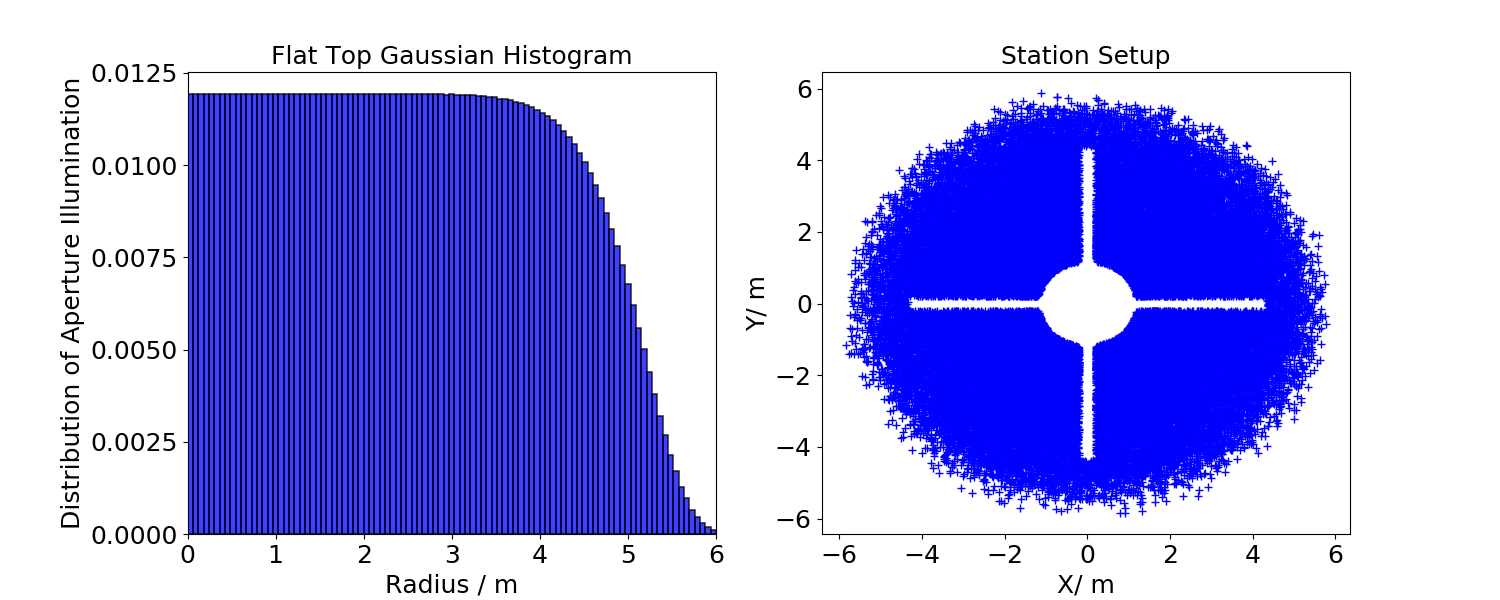
\includegraphics[width=6.0in]{c4/dhist_1} %   
%     \vspace*{1mm}
     \caption{The aperture illumination of dish-like surface is modelled using $80000$ dipoles.
        LEFT PLOT: The \enquote*{flat-top Gaussian} radial distribution of dipole positions, mimicking a realistic aperture illumination where 
        the dipoles get less dense towards the edge of the dish.
        RIGHT PLOT: The resulting 2D dipole distribution  with a mask applied to mimic aperture blockage.}        
    \label{fig:layout}
   \end{figure}
 \FloatBarrier 
%%
The parameters of the Super Gaussian distribution, $s$ and $\beta$ control the width of the distribution and the aggressiveness of the taper. 
 The values adopted in this work to produce the  radial distribution in the figure are $s = 0.82$ and  $\beta = 12.0$.\\
 %%
\noindent  We imitate the aperture blockage in point~\ref{itm:d2} by simply masking the 2D positions. This ultimately results in the dipole distribution 
shown in Fig.~\ref{fig:layout}, right. 
This dipole distribution is then fed into OSKAR as the \enquote*{station layout}. For a given set of observational parameters (in particular, pointing at zenith), 
OSKAR then computes the station primary beam response\footnote{{This takes $\approx 3 \, \rm minutes$} on a Tesla K40 GPU.}.
The resulting \emph{Jones matrix} elements are shown in Fig.~\ref{fig:jns}. 
Note how the beam pattern is broadly similar to that expected from a prime-focus dish. In particular, the first side-lobe shows the four-fold symmetry caused by the strut blockage.
The presence of the phase component in Fig.~\ref{fig:osk_im} clearly shows that the so-called ideal beam is not that perfect since we are randomly placing the dipoles in 
the KAT-7 dish-like form, hence, the norminal $X$ and $Y$ dipoles are not directly orthogonal. In effect, we get the maximum $rmse \approx 0.10 \%$ perturbed inaccuracies on 
the dish surface as reported in Fig.~\ref{fig:err}.
%
% 

\begin{figure}[H]
     \centering
     \begin{subfigure}[b]{0.7\textwidth}
         \centering
         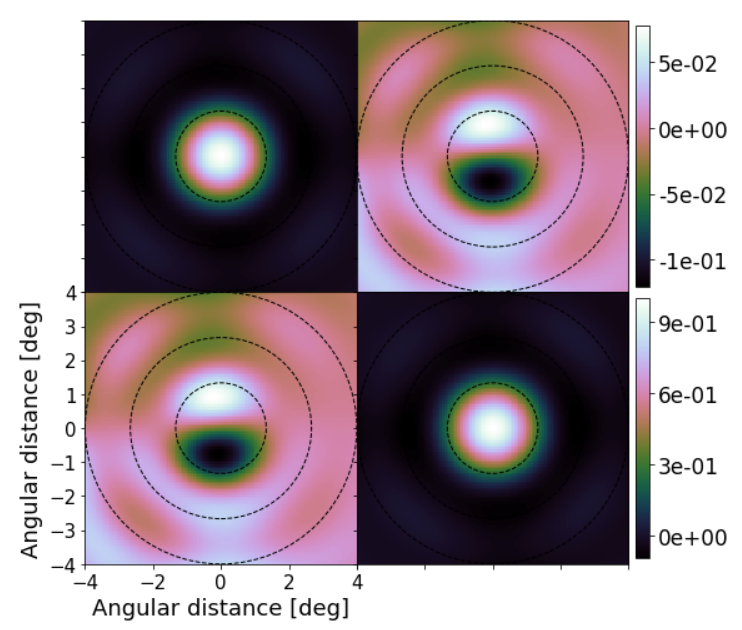
\includegraphics[width=\textwidth]{sec2jones/osk_re}
         \caption{}
         \label{fig:osk_re}
     \end{subfigure}
     \hfill
     \begin{subfigure}[b]{0.7\textwidth}
         \centering
         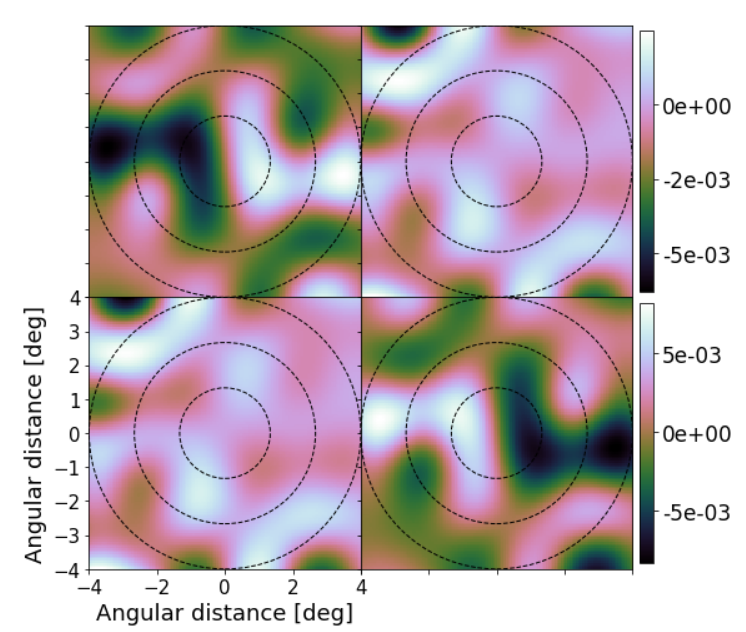
\includegraphics[width=\textwidth]{sec2jones/osk_im}
         \caption{}
         \label{fig:osk_im}
     \end{subfigure}
     \caption{Jones matrix representation of the KAT-7-like beams produced by OSKAR and shown at $1$ GHz: (a) real part (b) imaginary part. 
        The intensity of the imaginary parts increases with fewer dipoles and becomes smaller when more dipoles are used. The four panels in (a) and (b) show
        XX (top-left), XY (top-right), YX (bottom-left) and YY (bottom-right). Note that the notations X and Y denote the horizontal and vertical linear polarised beams.}\label{fig:jns}
\end{figure}
\FloatBarrier
%%
 \begin{figure}
\begin{minipage}[H]{\linewidth}
      \centering
      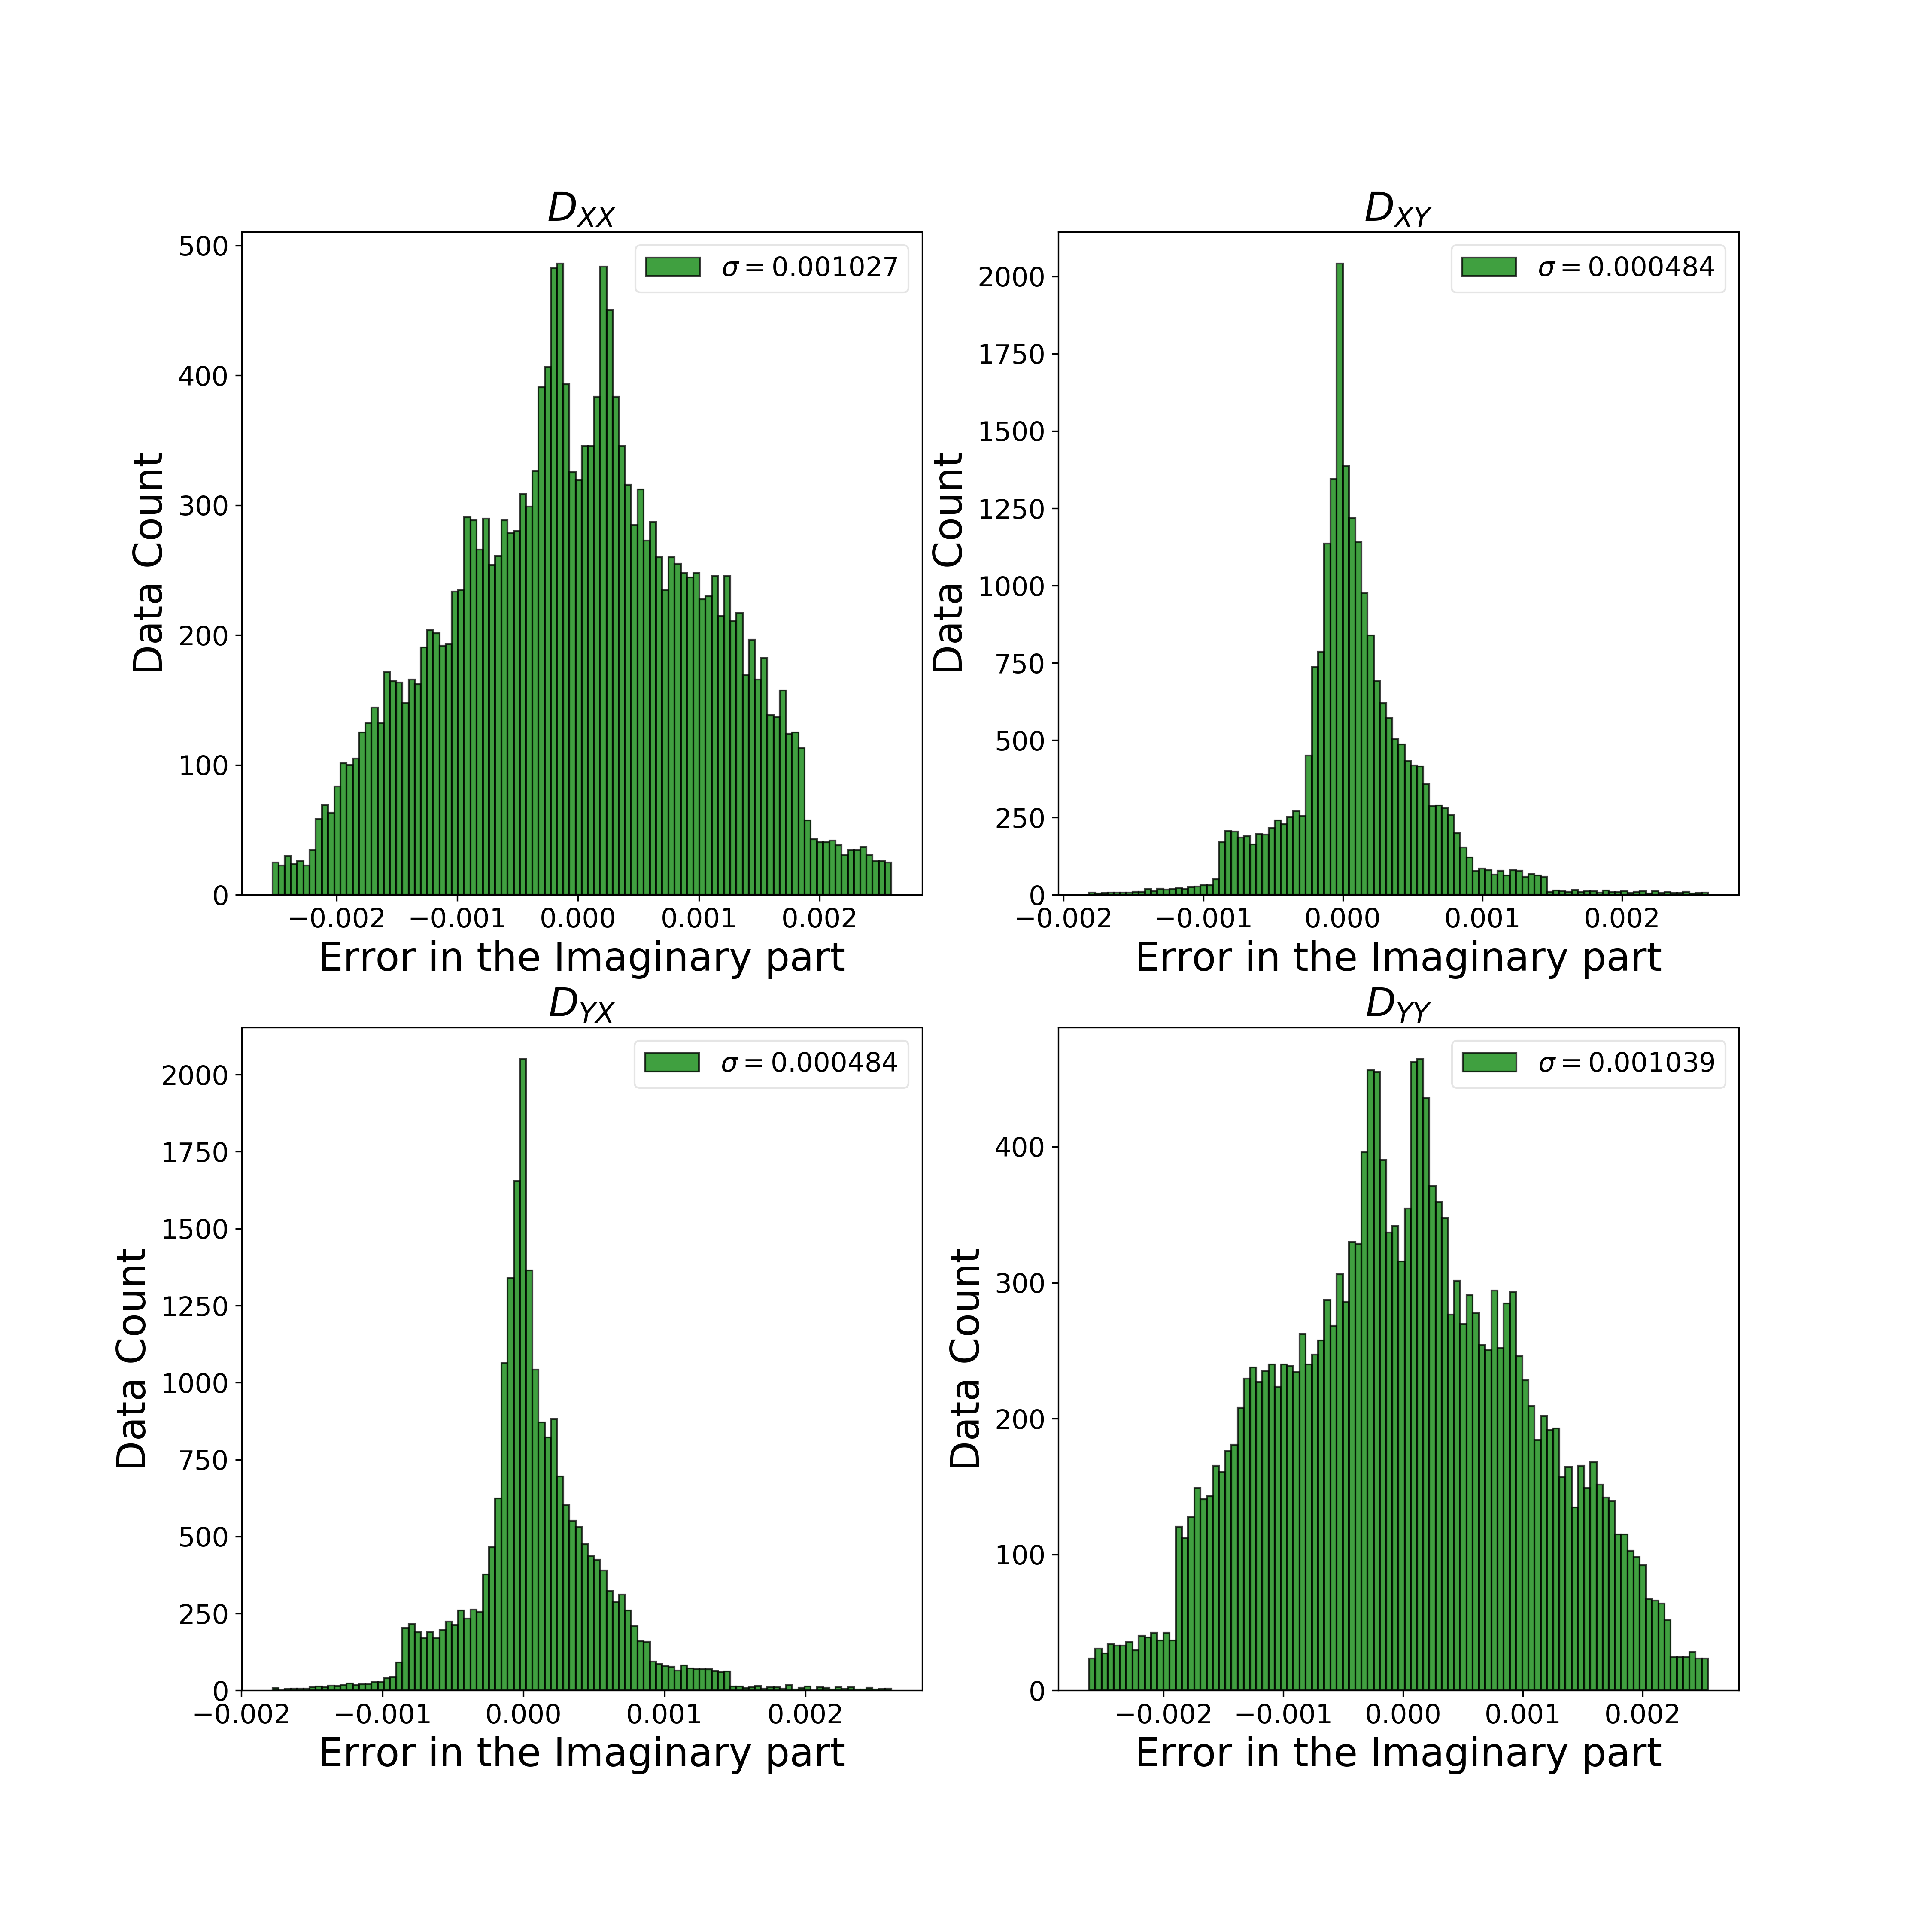
\includegraphics[width=5.8in]{sec2jones/hist_ANT1_chan0} %
    \end{minipage}
    \vspace*{-10mm}
     \caption{Histogram plots of the imaginary components in Fig.~\ref{fig:jns} showing the distribution of inaccuracies on the KAT-7 dish-like surface.}     	    \label{fig:err}
    \end{figure}
    \FloatBarrier
 
% --------------------------------------------------------------------------------------------------------------------------------

Note that the Jones \citep{1948JOSA...38..671J, 1942JOSA...32..486J} formalism, initially designed to describe optical polarization, was used 
by \cite{1996A&AS..117..137H} in radio interferometry  and further extended to direction-dependent effects by \cite{2011A&A...527A.106S}. In the next section,
we adapt the derivations of the latter two works.
%%

% +++++++++++++++++++++++++++++++++++++++++++
\subsection{Jones and Mueller matrices}       \label{sec:mueller}
% ++++++++++++++++++++++++++++++++++++++++++++
%%

An electromagnetic plane wave propagating along axis $z$ can be described, at any point in space and time, by two complex amplitudes, $e_x$ and $e_y$. 
Conventionally, we arrange these into a column vector, $\bm{e} = [e_x,e_y]^T$. A single-dish observation aims to measure the pairwise coherencies of these amplitudes:

\begin{equation}  \label{eq:pairwise}
\bm{x} = \left [ \begin{array}{c} \langle e_x e_x^* \rangle \\ \langle e_x e_y^* \rangle \\ \langle e_y e_x^* \rangle \\ \langle e_y e_y^* \rangle \end{array} \right ] =
\langle \bm{e} \circledast \bm{e}^* \rangle,
\end{equation}

\noindent where $\langle\cdot\rangle$ represents the average over a time/frequency interval, and $\otimes$ is the outer (or Kronecker) product operator.
From these measured coherencies, the Stokes parameters $IQUV$ (written as a column vector $\bm{s}$) may be derived, by definition, as \citep{1980poet.book.....B}:

\begin{equation}  \label{eq:stokes}
\bm{s} = \left [ \begin{array}{c} I \\ Q\\ U \\ V \end{array} \right ] =
\left [ \begin{array}{c} \langle e_x e_x^* \rangle + \langle e_y e_y^* \rangle \\ \langle e_x e_x^* \rangle - \langle e_y e_y^* \rangle \\
\langle e_x e_y^* \rangle + \langle e_y e_x^* \rangle \\ -\imath (\langle e_x e_y^* \rangle - \langle e_y e_x^* \rangle ) \end{array} \right ]
\end{equation}


\noindent We can rewrite this in terms of a $4\times4$ conversion matrix $\bm{S}^{-1}$ as\footnote{This follows \cite{2011A&A...527A.106S} in defining $\bm{S}$ as 
the conversion matrix between Stokes vectors and coherency vectors, $\bm{v}=\bm{Ss}$. Conversely, $\bm{S}^{-1}$ operates in the opposite direction.
Note that \cite{1996A&AS..117..137H} use $\bm{T}$ to refer to $\bm{S}^{-1}$.}:
%%

% \newpage
\begin{equation}  \label{eq:mconversion}
\bm{s} = \left[ \begin{array}{cccc}
                         1 & 0 & 0 & 1 \\
                         1 & 0 & 0 & -1 \\
                         0 & 1 & 1 & 0 \\
                         0 & -\imath & \imath & 0
                         \end{array} \right] \bm{x} = \bm{S}^{-1} \bm{x}.
\end{equation}

What the instrument actually measures is a set of pairwise correlations between two voltages induced by the EM field on two orthogonal mode feeds, $v_a$ and $v_b$. 
The Jones formalism assumes that these are linearly related to the EM field (i.e. that all signal propagation effects are linear). 
This can be written as $\bm{v}=\bm{J} \bm{e}$, where $\bm{v}$ is a column vector of the two voltages, and the $2\times 2$ \emph{Jones matrix} $\bm{J}$ 
describes signal propagation. The \emph{measured} coherency $\bm{x}'$ can then be written as:

% \newpage
\begin{equation}
\bm{x}' = \langle \bm{v} \circledast \bm{v}^* \rangle = (\bm{J} \circledast \bm{J}^* ) \langle \bm{e} \circledast \bm{e}^* \rangle =
(\bm{J} \circledast \bm{J}^* ) \bm{x},
\end{equation}

\noindent and the measured Stokes parameter vector $\bm{s}'$ relates to the original Stokes vector via the so-called \emph{Mueller matrix} $\bm{M}$:

\begin{equation} \label{eq:simpl}
\bm{s}' = \bm{M} \bm{s} = \bm{S}^{-1} (\bm{J} \circledast \bm{J}^* ) \bm{S} \bm{s}
\end{equation}

\noindent For the purposes of this work, we ignore all propagation effects except the primary beam. 
%%
   
\noindent Therefore, expanding the Jones terms in Equation~\ref{eq:simpl}, we can measure the full elements of $\bm{M}$, thus:
%%
\begin{eqnarray} \bm{J} \circledast \bm{J}^* = \left( \begin{array}{cccc}
                         j_{\rm xx}\,j_{\rm xx}^* & j_{\rm xx}\,j_{\rm xy}^* & j_{\rm xy}\,j_{\rm xx}^* & j_{\rm xy}\,j_{\rm xy}^* \\
                         j_{\rm xx}\,j_{\rm yx}^* & j_{\rm xx}\,j_{\rm yy}^*  & j_{\rm xy}\,j_{\rm yx}^* & j_{\rm xy}\,j_{\rm yy}^* \\
                         j_{\rm yx}\,j_{\rm xx}^* & j_{\rm yx}\,j_{\rm xy}^* & j_{\rm yy}\,j_{\rm xx}^* & j_{\rm yy}\,j_{\rm xy}^* \\
                         j_{\rm yx}\,j_{\rm yx}^* & j_{\rm yx}\,j_{\rm yy}^* & j_{\rm yy}\,j_{\rm yx}^* & j_{\rm yy}\,j_{\rm yy}^*
                         \end{array} \right) \label{eq:fr19} \end{eqnarray}
                         %
                         
\noindent  If we substitute Equation~\ref{eq:fr19} into~\ref{eq:simpl}, we can then expand $\bm{M}$ in terms of Jones matrix elements:
%
\begin{subequations}\label{eq:fr20}
  \begin{align}
  m_{\rm II} & = (j_{\rm xx}j_{\rm xx}^{*}\, + j_{\rm xy}j_{\rm xy}^{*}\, + j_{\rm yx}j_{\rm yx}^{*}\, + j_{\rm yy}j_{\rm yy}^{*})/2  	\label{eq:fr20a}\\
  m_{\rm IQ} & = (j_{\rm xx}j_{\rm xx}^{*}\, - j_{\rm xy}j_{\rm xy}^{*}\, + j_{\rm yx}j_{\rm yx}^{*}\, - j_{\rm yy}j_{\rm yy}^{*})/2 	 \label{eq:fr20b}\\
  m_{\rm IU} & = (j_{\rm xx}j_{\rm xy}^{*}\, + j_{\rm xy}j_{\rm xx}^{*}\, + j_{\rm yx}j_{\rm yy}^{*}\, + j_{\rm yy}j_{\rm yx}^{*})/2  	\label{eq:fr20c}\\
  m_{\rm IV} & = i(j_{\rm xx}j_{\rm xy}^{*}\, + j_{\rm yx}j_{\rm yy}^{*}\, - j_{\rm xy}j_{\rm xx}^{*}\, - j_{\rm yy}j_{\rm yx}^{*})/2  	\label{eq:fr20d}\\
  m_{\rm QI} & = (j_{\rm xx}j_{\rm xx}^{*}\, + j_{\rm xy}j_{\rm xy}^{*}\, - j_{\rm yx}j_{\rm yx}^{*}\, - j_{\rm yy}j_{\rm yy}^{*})/2  	\label{eq:fr20e}\\
  m_{\rm QQ} & = (j_{\rm xx}j_{\rm xx}^{*}\, - j_{\rm xy}j_{\rm xy}^{*}\, - j_{\rm yx}j_{\rm yx}^{*}\, + j_{\rm yy}j_{\rm yy}^{*})/2  	\label{eq:fr20f}\\
  m_{\rm QU} & = (j_{\rm xx}j_{\rm xy}^{*}\, + j_{\rm xy}j_{\rm xx}^{*}\, - j_{\rm yx}j_{\rm yy}^{*}\, - j_{\rm yy}j_{\rm yx}^{*})/2 	\label{eq:fr20g}\\
  m_{\rm QV} & = i(j_{\rm xx}j_{\rm xy}^{*}\, - j_{\rm yx}j_{\rm yy}^{*}\, - j_{\rm xy}j_{\rm xx}^{*}\, - j_{\rm yy}j_{\rm yx}^{*})/2 	\label{eq:fr20h}\\
  m_{\rm UI} & = (j_{\rm xx}j_{\rm yx}^{*}\, + j_{\rm yx}j_{\rm xx}^{*}\, + j_{\rm xy}j_{\rm yy}^{*}\, + j_{\rm yx}j_{\rm xy}^{*})/2 	\label{eq:fr20i}\\
  m_{\rm UQ} & = (j_{\rm xx}j_{\rm xy}^{*}\, - j_{\rm xy}j_{\rm xx}^{*}\, + j_{\rm yx}j_{\rm yy}^{*}\, + j_{\rm yy}j_{\rm yx}^{*})/2  	\label{eq:fr20j}\\
  m_{\rm UU} & = (j_{\rm xx}j_{\rm yy}^{*}\, + j_{\rm yy}j_{\rm xx}^{*}\, + j_{\rm xy}j_{\rm yx}^{*}\, + j_{\rm yx}j_{\rm xy}^{*})/2 	 \label{eq:fr20k}\\
  m_{\rm UV} & = i(j_{\rm xx}j_{\rm yy}^{*}\, + j_{\rm yx}j_{\rm xy}^{*}\, - j_{\rm yy}j_{\rm xx}^{*}\, - j_{\rm xy}j_{\rm yx}^{*})/2 	\label{eq:fr20l}\\
  m_{\rm VI} & = i(-j_{\rm xx}j_{\rm yx}^{*}\, + j_{\rm yx}j_{\rm xx}^{*}\, - j_{\rm xy}j_{\rm yy}^{*}\, + j_{\rm yy}j_{\rm xy}^{*})/2  	\label{eq:fr20m}\\
  m_{\rm VQ} & = i(-j_{\rm xx}j_{\rm yx}^{*}\, + j_{\rm yx}j_{\rm xx}^{*}\, + j_{\rm xy}j_{\rm yy}^{*}\, - j_{\rm yy}j_{\rm xy}^{*})/2 	\label{eq:fr20n}\\
  m_{\rm VU} & = i(-j_{\rm xx}j_{\rm yy}^{*}\, + j_{\rm yy}j_{\rm xx}^{*}\, - j_{\rm xy}j_{\rm yx}^{*}\, + j_{\rm yx}j_{\rm xy}^{*})/2 	 \label{eq:fr20o}\\
  m_{\rm VV} & = (j_{\rm xx}j_{\rm yy}^{*}\, - j_{\rm yx}j_{\rm xy}^{*}\, + j_{\rm yy}j_{\rm xx}^{*}\, - j_{\rm xy}j_{\rm yx}^{*})/2  	\label{eq:fr20p} 
 \end{align}
%  \phantom{\hspace{1cm}} 
\end{subequations}
%
The sixteen elements in Equations~\ref{eq:fr20a} to~\ref{eq:fr20p} are the complete PBs of a radio telescope (as shown in Fig.~\ref{fig:truosk}) produced from the complex beams 
(see Fig.~\ref{fig:jns}). The DD effect of the PB will cause each element in Equation~\ref{eq:fr20} to produce different matrices. 
If we substitute the elements in Equation~\ref{eq:fr20} into Equation~\ref{eq:simpl}, we get the measured Stokes parameters in Equation~\ref{eq:fr21}:

\begin{eqnarray} \left( \begin{array}{c}
                         S'_{I}\\
                         S'_{Q}\\
                         S'_{U}\\
                         S'_{V}
                        \end{array} \right) =
\left( \begin{array}{cccc}
                        m_{II} & m_{IQ} & m_{IU} & m_{IV} \\
                        m_{QI} & m_{QQ} & m_{QU} & m_{QV} \\
                        m_{UI} & m_{UQ} & m_{UU} & m_{UV} \\
                        m_{VI} & m_{VQ} & m_{VU} & m_{VV} \end{array} \right)                     
                     \left( \begin{array}{c}
                         S_{I}\\
                         S_{Q}\\
                         S_{U}\\
                         S_{V}
                        \end{array} \right)  \label{eq:fr21}
\end{eqnarray} 

% %%
% \begin{equation}
% \bm{s}'_\mathrm{tot} = \iint\limits_{lm} \bm{M}(l,m) \bm{s}(l,m) \mathrm{d}l \mathrm{d}m,
% \end{equation}
% 
% \noindent where the integration is, in principle, over the entire celestial sphere, but in practice, since the Mueller matrix becomes negligibly 
% small outside of a certain FoV, it can be replaced by a 2D integral over the tangent plane $lm$.
% %%


Note the physical meaning of the matrix elements. The on-diagonal terms of the Jones matrix describe the sensitivity of each feed, as a function of direction, to its matched 
EM field component. The off-diagonal terms describe leakage, i.e. the sensitivity of the feed to the nominally orthogonal EM field component. This leakage is due to mechanical
and electronic imperfections in the antennas and feeds. The diagonal terms of the Mueller matrix describe the sensitivity of the measured Stokes $IQUV$ components to their true counterparts, 
as a function of direction. The off-diagonal terms describe spurious leakage between the measured Stokes components. We can schematically write this as;
% \newpage
$$ \bm{M}  =
\left[ \begin{array}{cccc}
  I \rightarrow I' & Q \rightarrow I' & U \rightarrow  I' & V \rightarrow  I' \\
  I \rightarrow Q' & Q \rightarrow Q' & U \rightarrow  Q' & V \rightarrow  Q'\\
  I \rightarrow U' & Q \rightarrow U' & U \rightarrow  U' & V \rightarrow  U'\\
  I \rightarrow V' & Q \rightarrow V' & U \rightarrow  V' & V \rightarrow  V'
\end{array} \right]
$$


\begin{figure}
  \centering
  \begin{minipage}[H]{\linewidth}
     \begin{subfigure}[b]{0.8\textwidth}
      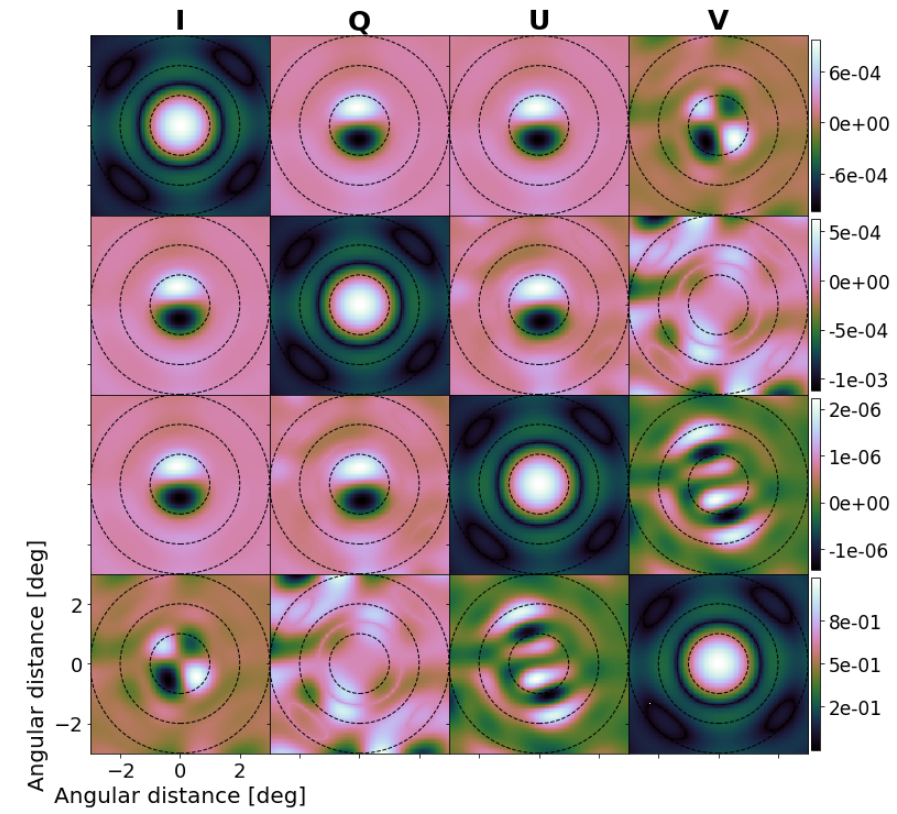
\includegraphics[width=\textwidth]{sec2oskbms/osk_trumueller}
                \caption{}
                \label{fig:truosk1}
        \end{subfigure}
        \qquad
        \begin{subfigure}[b]{0.8\textwidth}
 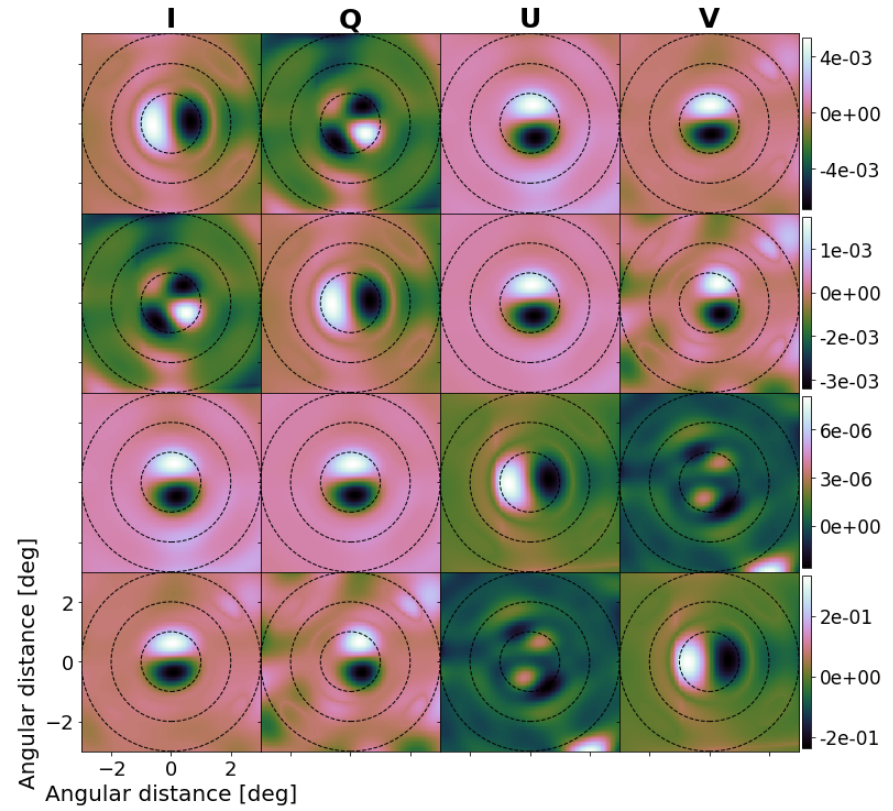
\includegraphics[width=\textwidth]{sec2oskbms/osk_tru-gpmueller}
                \caption{}
               \label{fig:truosk2}
        \end{subfigure}
%         
\end{minipage}
  \end{figure}
  \FloatBarrier
  
 %% 
  \begin{figure}
\ContinuedFloat
\centering
 \begin{minipage}[H]{\linewidth}
\begin{subfigure}[b]{0.8\textwidth}
      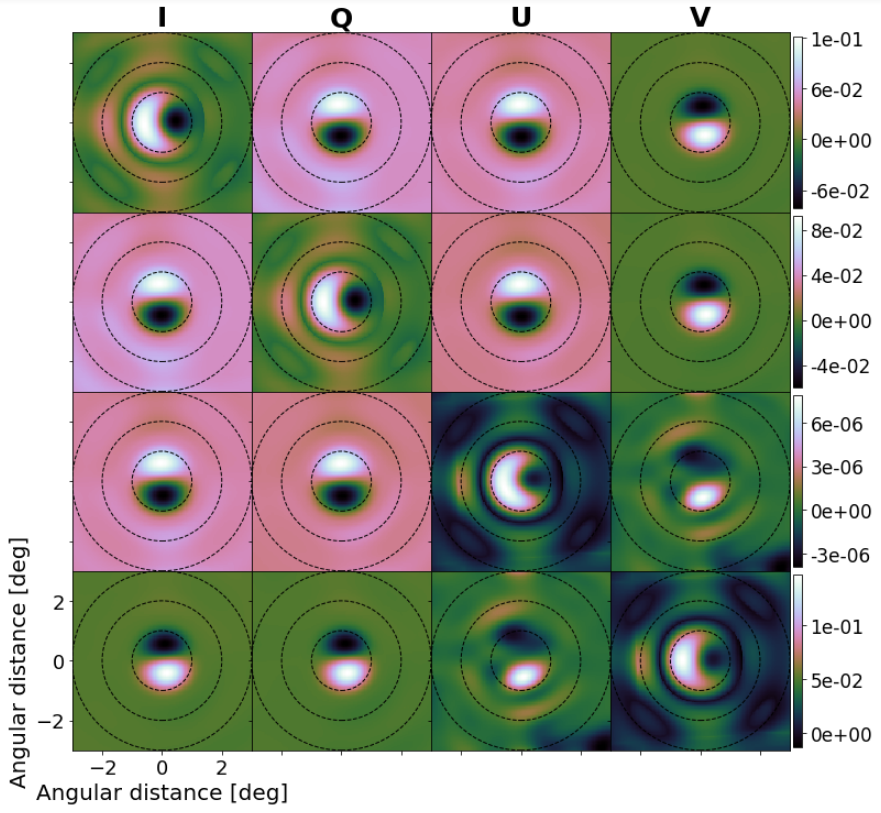
\includegraphics[width=\textwidth]{sec2oskbms/osk_tru-xymueller}
                \caption{}
                \label{fig:truosk3}
        \end{subfigure}
        \qquad
        \begin{subfigure}[b]{0.8\textwidth}
         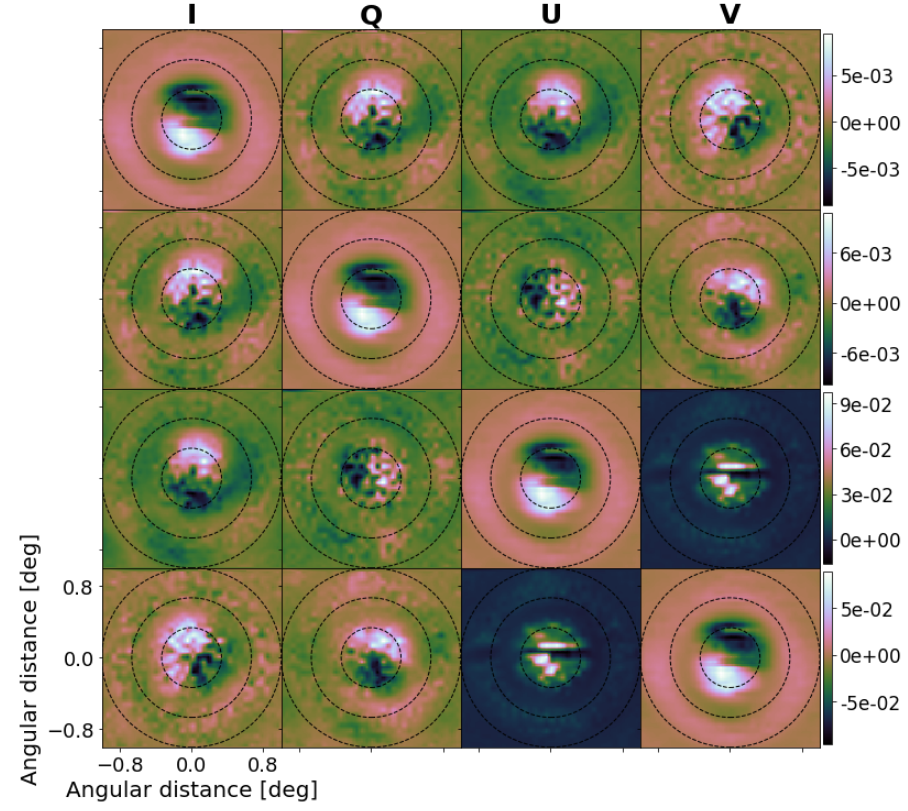
\includegraphics[width=\textwidth]{sec2realbms/vla-diffmueller}
                \caption{}
               \label{fig:truosk4}
        \end{subfigure}
         \end{minipage}
    \caption{\small{ Mueller matrix representations of full polarization beams produced at $1\, \mathrm{GHz}$
    (a) $4 \times 4$ images of KAT-7 uncorrupted OSKAR beams.
    (b) Fractional differences between the uncorrupted OSKAR beams in Fig.~\ref{fig:truosk1} and the gain and phase error beams in appendix~\ref{fig:A1a} 
     (c) Fractional differences between uncorrupted OSKAR beams in Fig.~\ref{fig:truosk1} and the dipole orientation error beams in  appendix~\ref{fig:A1b}.
     (d) Fractional differences between VLA holography measured beams in   Figs.~\ref{fig:A2a} and~\ref{fig:A2b}.}}      
	    \label{fig:truosk}
  \end{figure}
  \FloatBarrier

% +++++++++++++++++++++++++++++++++++++++++++
\subsection{Primary Beam Perturbation}       \label{sec:perturb}
% ++++++++++++++++++++++++++++++++++++++++++++
%%

For the purpose of this research, we try to introduce some distortions on the simulated OSKAR beams for IM experiment.
The first type is to corrupt both the gain and phase of the beam in a systematic manner. Here, we can do this with OSKAR by simulating
the gain and phase of each element so that the weight of the beamformer $W_{\rm B}$ at a particular time $t$, for a given pointing direction $(\vartheta_{\rm B}, \varphi_{\rm B})$
and dipole locations $(\upsilon_{\rm 1}, \upsilon_{\rm 2}, \upsilon_{\rm 3})$ is given in \citep{ansah2018simulations} as:

% EQ11
\begin{equation} W_{\rm B} (\bm{\upsilon}) =  (G_{\rm B}^{ 0} + G_{\rm B}^{error}) W_{B}^{geo}(\bm{\upsilon})\mathrm{e}^{j\left(\varphi_{\rm B}^{0} + \varphi_{\rm B}^{error} \right)} \label{eq:q11} \end{equation} 
%%


% The modelled beams produced in this chapter are corrupted with two kinds of errors. The first error type is the introduction of systematic and time-variable 
% gain and phase errors. The nominal purpose of this in OSKAR is to simulate per-element gain and phase error before the beamformer, so that the beam-forming weight $B^{w}$, 
% for a particular beam direction $(\theta_{bm}, \phi_{bm})$, with dipole position $(x, y, z)$ and time $t$ becomes;%%
% %%
% % EQ11
% \begin{equation} W_{\rm B} =  W_{B}^{geo}(u)(G_{0} + G_{error})\exp(j\left[\phi_{0} + \phi_{error}\right]) \label{eq:q11} \end{equation} 
% %%
\noindent The parameters  $\bm{\upsilon} = (\vartheta_{\rm B}, \varphi_{\rm B}, \upsilon_{\rm 1}, \upsilon_{\rm 2}, \upsilon_{\rm 3}, t)$, 
$G_{\rm B}^{error}$ and $\varphi_{\rm B}^{error}$ use the Gaussian function to generate deterministic random numbers at step-time $t$. We then combine these
parameters with $G_{\rm B}^{ 0}$ (the gain), $\varphi_{\rm B}^{0}$ (phase) and the geometrical kernel function $W_{B}^{geo}$, to obtain the array factor for beam evaluation.
%%
For the purpose of our \enquote{disk-like} simulation, we introduced $5^\circ$ 
phase error and $10 \%$ gain error into the beam-forming weight to distort the beams as shown in Fig.~\ref{fig:A1a}. These types of errors represent imperfections 
in the parabolic reflector surface (which, in real life, result in amplitude and phase errors over the aperture).
%%
The second perturbation is to introduce positional errors per element. Note that for ideal situation, both dipoles $(x,y)$ are orthogonal and the angular differences 
will be zero. However, displacing the dipoles from its nominal positions ($\sim 1^\circ$) will definitely produce an angular difference of being greater than zero, hence, creating a
systematic error in the feed angle and the effect of this is presented in  Fig.~\ref{fig:A1b}. Here, what we do is to indicate the Euler angles of the feeds of the nominal $x$ and $y$ dipoles in each station directory. These angles depict the differences from zero, since in the ideal case  both dipoles are expected to be  orthogonal and in the plane of the station platform.
%%
Figs.~\ref{fig:truosk2} and~\ref{fig:truosk3} 
show the beam errors produced by computing the differences between the true modelled beams in Fig.~\ref{fig:truosk1} and the two distorted beams in Figs.~\ref{fig:A1a} 
and~\ref{fig:A1b} respectively. The on-diagonal components of these beam errors represent the residual leakages and the off-diagonals show the residual systematic leakages. 
The maximum residual leakages produced in Figs.~\ref{fig:truosk2} and~\ref{fig:truosk3} are $\simeq 20 \%$ and $10 \%$ respectively.
%%

%%
Another thing that we considered in this work is to apply the JVLA holography beams to measure the degree of beam perturbation. The numerical scheme used to generate 
the JVLA beams in Figs.~\ref{fig:A2a} and~\ref{fig:A2b} is described in the EVLA Memo \citep{2015Rick} which involves the use of Fourier transform to determine the far-field 
beam pattern of an antenna. Fig.~\ref{fig:truosk4} is the residual error of the JVLA beams, producing $\simeq 10 \%$ leakage. Therefore, the systematic leakage in the holography
beams indicates that the simulated perturbations introduced in the OSKAR beams  are actually practical. 
%%

Now that we are abreast with the model of the instrument, we continue to show how we apply these beams to the simulated full-sky maps discussed in Chapter~\ref{Chapter3}.
%%

\section{Convolution of Foreground Maps}    \label{sec:convolution}
%%%

 %
Mathematically, convolution is an  operator that interpolates two expressions $\varUpsilon_{\rm \alpha}$ and $\varUpsilon_{\rm \beta}$ 
to produce a third function $\chi$ 
that is typically viewed as a modification of one of the original functions. Consider $C_{v}(\varsigma)$ to be the convolution of $ \Psi_{\rm \alpha}(\varsigma)$
with $ \Psi_{\rm \beta}(\varsigma)$, then its Fourier pair  $\chi(\nu)$, is the product of $\varUpsilon_{\rm \alpha} (\nu)$ and $\varUpsilon_{\rm \beta} (\nu)$ which define the 
Fourier pairs of $ \Psi_{\rm \alpha}(\varsigma)$ and $ \Psi_{\rm \beta}(\varsigma)$ respectively. Thus,
%
% EQ1
\begin{equation}  \Psi_{\rm \alpha}(\varsigma)\, \odot\, \Psi_{\rm \beta}(\varsigma) \, \rightleftharpoons \, \varUpsilon_{\rm \alpha} (\nu). \varUpsilon_{\rm \beta} (\nu) \label{eq:u31} \end{equation}
%

\noindent where the symbol $\odot$ denotes the convolution operator. By definition,
%% EQ2
\begin{equation}
 \begin{aligned}
  C_{v}(\varsigma) &=  \Psi_{\rm \alpha}(\varsigma) \,\odot \,  \Psi_{\rm \beta}(\varsigma)\\
  &= \int_{- \infty}^{\infty}\,  \Psi_{\rm \alpha}(\varsigma')  \Psi_{\rm \beta}(\varsigma - \varsigma') \mathnormal{d\varsigma} 
  \end{aligned}
  \label{eq:u32}
\end{equation}
%
Taking the Fourier transform of both sides in Equation~\ref{eq:u32}, we get:
% % EQ3
\begin{equation}
\begin{aligned}
 \chi(\nu) &= \int_{- \infty}^{\infty} C_{v}(\varsigma)\mathnormal{e}^{-2\pi j \nu \varsigma}\mathnormal{d\varsigma}\\
 &= \int_{- \infty}^{\infty} \int_{- \infty}^{\infty} \,
  \Psi_{\rm \alpha}(\varsigma')  \Psi_{\rm \beta}(\varsigma - \varsigma')\mathnormal{e}^{-2\pi j \nu \varsigma}\mathnormal{d\varsigma'\, d\varsigma}
 \end{aligned}
   \label{eq:u33}
\end{equation}
%
Let $ y = \varsigma - \varsigma' \, \Rightarrow \, \mathnormal{dy} = \mathnormal{d\varsigma} $
%% EQ4
\begin{equation}
  \chi(\nu) =  \int_{- \infty}^{\infty} \int_{- \infty}^{\infty} \,   \Psi_{\rm \alpha}(\varsigma')  \Psi_{\rm \beta}(y)\mathnormal{e}^{-2\pi j\nu(\varsigma' + y)}
  \mathnormal{d\varsigma'} \mathnormal{dy}
   \label{eq:u34}
\end{equation}
%
Equation~\ref{eq:u34} can therefore be separated to give:

% EQ5
\begin{equation}
 \begin{aligned}
  \chi(\nu)  & =\,  \int_{- \infty}^{\infty} \,   \Psi_{\rm \alpha}(\varsigma')\mathnormal{e}^{-2\pi j \nu \varsigma'} \mathnormal{d\varsigma'}.
  \int_{- \infty}^{\infty} \,  \Psi_{\rm \beta}(y)\mathnormal{e}^{-2\pi j \nu y} \mathnormal{dy} \\
   & =\,  \varUpsilon_{\rm \alpha}(\nu). \varUpsilon_{\rm \alpha}(\nu)
\end{aligned}
\label{eq:u35}
\end{equation}
%
Expressing the general definition in Equation~\ref{eq:u35} into $\rm 2D$ discrete form, we have:

%% EQ6
 \begin{equation}
   \begin{aligned}
   \chi(\nu_{\rm \alpha}, \nu_{\rm \beta}) &=   \Psi_{\rm \alpha}(\nu_{\rm \alpha}, \nu_{\rm \beta}) \,\odot \Psi_{\rm \beta}(\nu_{\rm \alpha}, \nu_{\rm \beta}) \\ 
  &= \, \sum_{m = - \infty}^{\infty} \sum_{n = - \infty}^{\infty} \,   \Psi_{\rm \alpha} (m - \nu_{\rm \alpha}, n - \nu_{\rm \beta}) \Psi_{\rm \beta}(m, n)
  \end{aligned}
\label{eq:u36} 
\end{equation}
%
In Equation~\ref{eq:u36}, the values $  \chi(\nu_{\rm \alpha}, \nu_{\rm \beta})$ of the discrete function $ \chi$ for any particular $ (\nu_{\rm \alpha}, \nu_{\rm \beta})$ follows by multiplying
each value $ \Psi_{\rm \beta}(m, n)$ of the discrete function $ \Psi_{\rm \beta}$ with a kernel function $ \Psi_{\rm \alpha} (m - \nu_{\rm \alpha}, n - \nu_{\rm \beta})$
between a particular 
$ (\nu_{\rm \alpha}, \nu_{\rm \beta})$ and varying $(m, n)$ where, $(- \infty \, < \, m, \, n \, <  \, + \infty)$. Thus, each value $  \chi(\nu_{\rm \alpha}, \nu_{\rm \beta})$ of the function 
$ \chi$ is a weighted mean of the values $ \Psi_{\rm \beta}(m, n)$ with weights $ \Psi_{\rm \alpha} (m - \nu_{\rm \alpha}, n - \nu_{\rm \beta})$ defined by the function
$ \Psi_{\rm \alpha}$. In this chapter, we apply similar approach to simulate the foreground of the sky.
To perform an IM experiment, the radio telescope(s) is pointed at different patches of the sky so that the instrument can measure the overall
intensity emerging from patches from the autocorrelation of the radio signal, as a function of frequency. In order to emulate this observation 
technique in our IM simulation, the discrete convolution in Equation~\ref{eq:q13} is used to measure the intensities of the full sky synchrotron 
maps in Fig.~\ref{fig:f1000}. Let $(\theta, \phi)$ denote the celestial coordinates of the foregrounds of the sky, such that $\bm{B}$ are the fully
polarised beams  and $\bm{f_{\rm sky}}$ are the foregrounds of the sky. We can then model the convolved foregrounds to be: 
 
%% EQ7
\begin{equation}	\label{eq:q13}  
\begin{aligned}  
  \bm{F^{conv}}(\theta, \phi) & =\,  \bm{B}(\theta, \phi) \, \odot \bm{f_{\rm sky}}(\theta, \phi) \\
  & = \sum_{ (\theta', \phi') = \,\lfloor \, (\theta, \phi) \, \rceil} \!\!\!  
  \bm{B}(\theta' - \theta, \phi' - \phi).\bm{f_{\rm sky}}(\theta', \phi')
\end{aligned} 
  \end{equation}
 % 
 
\noindent where  $ (\theta', \phi') \leq npix$ and the symbol $\lfloor \, \rceil$ denotes the nearest pixels. The measured foreground
pixel values $\bm{ F^{conv}}(\theta, \phi)$ of the discrete function $\bm{F^{conv}}$ for any particular $ (\theta, \phi)$ follows by 
multiplying each foreground pixel value $\bm{f_{\rm sky}}(\theta, \phi)$ of the discrete function $\bm{f_{\rm sky}}$ with a beam  $\bm{B}(\theta' - \theta, \phi' - \phi)$
between a particular $ (\theta', \phi')$ and varying $(\theta, \phi)$. Thus, each pixel value $\bm{ F^{conv}}(\theta, \phi)$ of the function $\bm{F^{conv}}$ is 
a weighted mean of the pixel values $\bm{f_{\rm sky}}(\theta, \phi)$ with weights $\bm{B}(\theta' - \theta, \phi' - \phi)$ defined by the function $\bm{B}$.

The convolution technique in Equation~\ref{eq:q13} is implemented in this work using the {\tt HEALPix} query disc function (Python package). 
This function is applied on the {\tt HEALPix} map (the full-sky map) with $Nside = 512$ to query all the nearby pixels that fall within the primary beamwidth for every pointing.
These query pixels are then convolved with the corresponding pixel values in the beam. So for each pointing, we get different query pixels even though there can be overlapping pixels
like the rings shown in Fig.~\ref{fig:implota}, as you point the beam to the next direction. To measure the exact intensity of the foreground, the convolved {\tt HEALPix} map is normalised by the power beam (Stokes I). For instance, in Equation~\ref{eq:q13}, if we let $\bm{B}$ to be the complete beams in Fig.~\ref{fig:truosk1}  and then replace $\bm{f_{\rm sky}}$ with Fig.~\ref{fig:f1000}, we generate $\bm{ F^{conv}}$ as shown in Fig.~\ref{fig:fgTrCnv}. We repeat the procedure, using the beams in Figs.~\ref{fig:A1a} and~\ref{fig:A1b} to obtain perturbed maps.  Similarly, doing same for the JVLA beams in Figs.~\ref{fig:A2a} and~\ref{fig:A2b}, we produce their corresponding  measured sky maps. In Fig.~\ref{fig:fgTrCnv}, we can observe that the spatial representation of the inclining maps from left to right are retained as that of the initial foreground images displayed in Fig.~\ref{fig:f1000}. This happens when we convolve the sky maps with the gain terms (i.e. $m_{\rm II}, m_{\rm QQ}, m_{\rm UU}$).

%%

In performing IM,  we are mostly curious about the absolute intensity of the foreground. This can be done by transforming the spatial representation of the convolved sky maps 
into spherical harmonics in order to estimate the power spectrum in a scale of moments ($l$). The next section presents the angular power spectrum described in \citep{ansah2018simulations}.
% actually interested in, is to measure the total intensity of a signal. Therefore, in Section~\ref{sec:spectrum},
%  we present a mathematical model of the convolved power spectrum using the angular power spectrum approach to describe the spatial distribution of the measured foregrounds in a spherical harmonic domain
%%

\begin{figure}
\centering
\begin{minipage}[H]{\linewidth}
       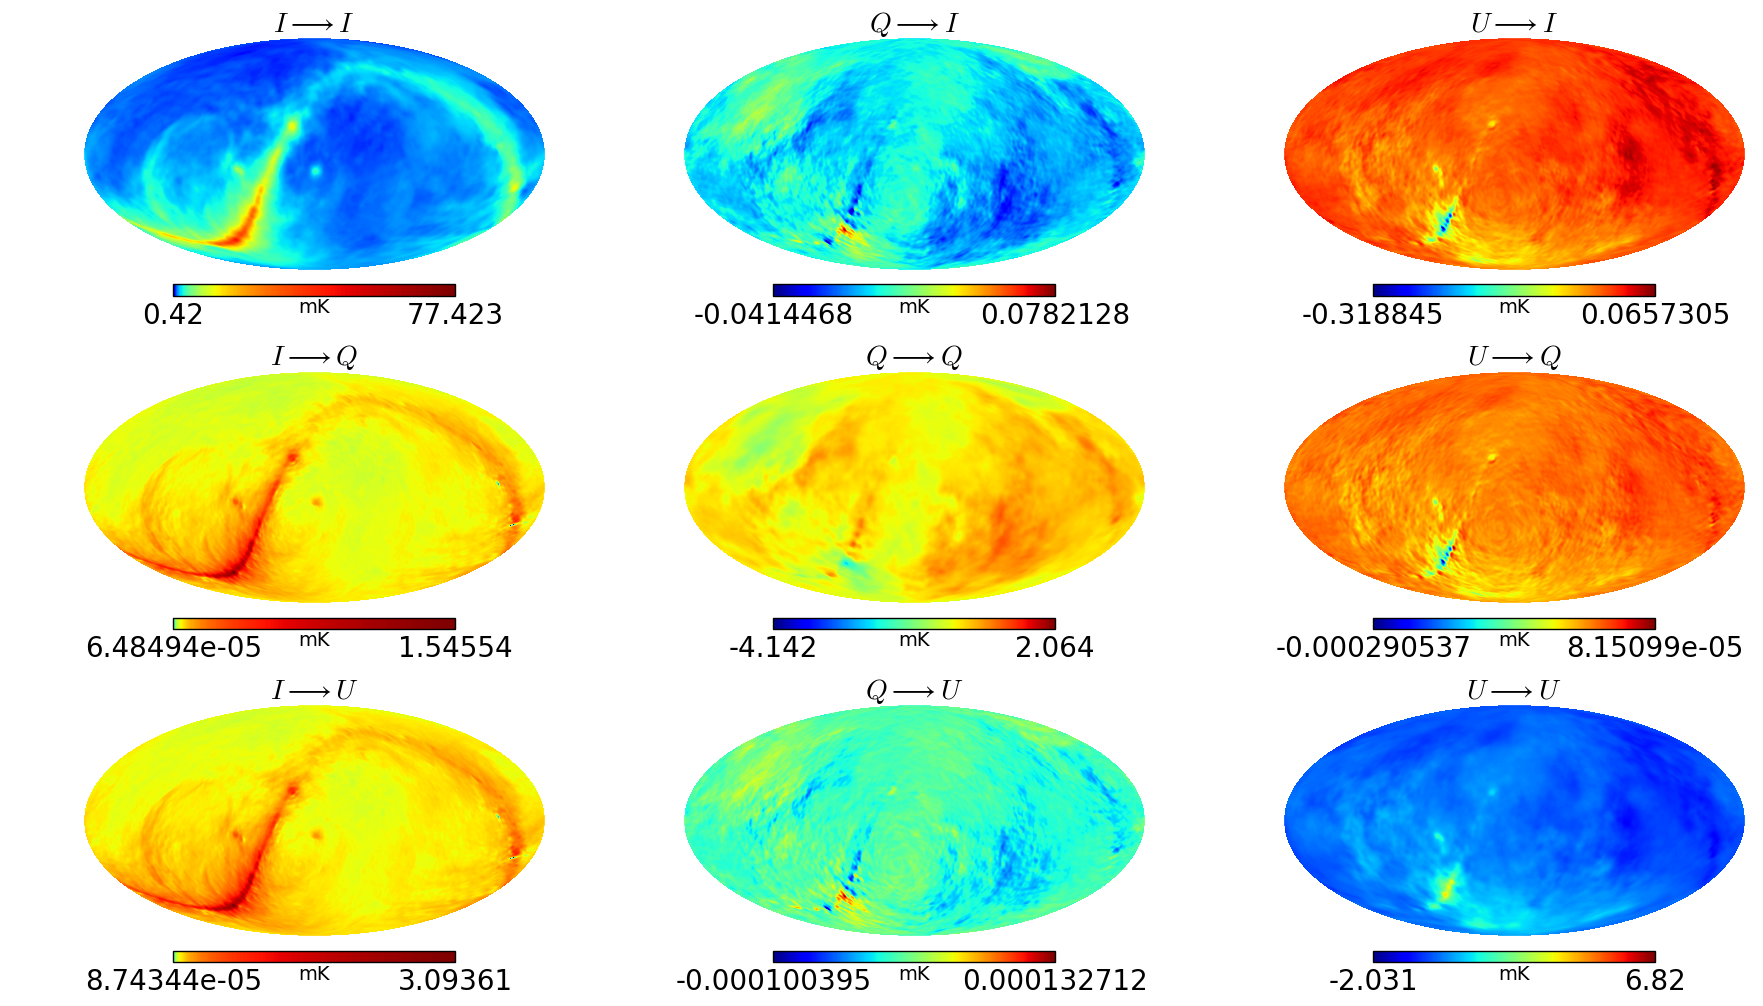
\includegraphics[width=6.6in]{sec3gp_conv/osk_Tr1}
      \end{minipage}
    \caption{Convolved full-sky polarization maps using the non-distorted OSKAR beams. 
    For example, we used the $m_{\rm II}$ beam in Fig.~\ref{fig:truosk1} to convolve Stokes $I$ in Fig.~\ref{fig:f1000} and produce the convolved map $I \rightarrow I$ , 
    then we used $m_{\rm QI}$ beam to convolve Stokes $Q$ to obtain the convolved map $Q \rightarrow I$, also, using the $m_{\rm UI}$ beam to convolve Stokes $U$ we produced the convolved map $U \rightarrow I$. The other convolved maps are produced in the same manner using their respective beams.} \label{fig:fgTrCnv}
\end{figure}
\FloatBarrier


% 
\subsection{Angular Power Spectrum}    \label{sec:spectrum}
%%  
In CMB studies \citep{2016MNRAS.457.1796A,2016A&A...588A..65K,2015aska.confE..35W,2006NewAR..50..854S,2006ApJ...645L..89S,1998PhRvD..57.5273W},
it is a common practice to characterise the distribution of flux in a sphere with the angular power spectrum. The same approach is employed in
this project to describe the diffuse foreground intensity over spherical harmonics $Y_{l,m}$.
%%

Consider the foreground of the sky is emitted by our own galaxy or the distribution galaxies emitting $21$ cm with an intensity equivalent to $ T(\hat{\sigma})$. We can measure the total source emission temperature $T(\hat{\sigma})$, in each sky pixel and represent the distribution as an expansion in 2D spherical harmonics:
%%

 %% EQ8
 \begin{equation}  	\label{eq:q14} 
                    T(\hat{\sigma}) = \mathop{\sum_{l\, = 0}^{\infty}\sum_{m\, = -l}^{l}} \, a_{lm}Y_{lm}(\hat{\sigma})
     \end{equation}
 %%

\noindent where $\hat{\sigma} \equiv (\psi, \xi)$ is the unit vector in some direction in the sky and $Y_{lm}(\hat{\sigma})$ are 
the spherical harmonic functions evaluated in the direction $\hat{\sigma}$, such that they form a complete orthonormal set 
on the unit sphere and can be expressed as:
%%

\begin{equation} 	\label{eq:q15}
            Y_{lm}(\psi ,\xi) = (-1)^m \, \sqrt{\frac{2l + 1}{4\pi} \, \frac{(l - m)!}{(l + m)!}}\, P_{ l}^{m}(\cos \psi)e^{im\xi} 
		      \end{equation}
%%

\noindent In Equation~\ref{eq:q15}, the indices $l = 0, \dots, \infty$ and $-l \leq m \geq l$ with $P_{ l}^{m}$ denoting the
Legendre polynomials. $l$ is known as the multipole which denotes a given angular scale $\gamma$ in the sky, where
$\gamma \simeq 180^{\circ}/l$. The coefficients $ a_{lm}$ in Equation~\ref{eq:q14},
 %% EQ44
 
 \begin{equation} 	  \label{eq:q16}
         a_{lm} = \int_{\psi = - \pi/2}^{\pi/2} \,\int_{\xi = 0}^{2\pi} \, T_{lm}(\hat{\sigma})Y_{lm}^{*}(\hat{\sigma})\mathnormal{{d\xi}{d\psi}}                            
		      \end{equation}
%
are related to what we normally do in the Fourier space.
%

Consider any two pixels, then the correlation function of the temperatures is expressed as;
 % EQ11
  \begin{equation}		\label{eq:q17}   
   C_{cr}(\Theta) = \langle T(\hat{\sigma_i})T(\hat{\sigma_j})\rangle \, , \quad \Theta = \sigma_{i}.\sigma_{j}   
  \end{equation}
%
 where the brackets $\langle \, \rangle$, denote averaging over $2l+1$ values of $m$. Equation~\ref{eq:q17} 
strictly relies on the separation angle between two sources as discussed in \citep[p. 78]{1997Schramm} and, therefore can be rewritten in terms of Legendre polynomials:
%
% EQ12
\begin{equation}  	 \label{eq:q18}
   C_{cr}(\Theta) = \mathop{\sum_{l\, = 0}}\, \frac{2l + 1}{4\pi}\,C_{l}P_{l}(\cos \Theta)  
  \end{equation}
  %%
  
\noindent From Equation~\ref{eq:q18}, we can estimate the statistical distribution of the angular power spectrum $\hat{C_l}$ of the entire sky in terms of $a_{lm}$:
 %
 % EQ13
 \begin{equation}  	\label{eq:q19}
  \hat{C_l} = \frac{1}{2l + 1}\, \mathop{\sum_{m}}\, |\hat{a_{lm}}|^{2} \, , \quad -l < m < l 	
\end{equation}
% 

In this work, we used \emph{anafast} in HEALPix library to compute the auto-power spectrum $\hat{C}_{l}$ of foregrounds of the sky
in Section~\ref{sec:convolution} by executing an approximate, discrete point-set quadrature on a sphere sampled at the HEALPix pixel centres.
Spherical harmonic transforms are then computed using recurrence relations for Legendre polynomials on co-latitude $\psi$ and Fast Fourier Transforms on longitude $\xi$.
%%

\section{Results and Analysis}    \label{sec:results}
 %%
The top three rows in Fig.~\ref{fig:fgGP} depict the total convolved full-sky images in Stokes parameters $I, Q$ and $U$. If we convolve the initial sky maps in Fig.~\ref{fig:f1000}
with the correct modelled beams in Fig.~\ref{fig:truosk1} and then put their respective Stokes terms together, we obtain the images in the first row. We repeat the steps
to produce the images in the second and third rows, but this time around, we use the false modelled beams in Fig.~\ref{fig:A1}.
% The measured full-sky maps of $\{I^{\rm T}, Q^{\rm T}, U^{\rm T} \}$ (reported in row $1$), $\{I_{}^{\rm GP}, Q_{}^{\rm GP}, U_{}^{\rm GP}\}$ (reported in row $2$) and
% $\{I_{}^{\rm XY}, Q_{}^{\rm XY}, U_{}^{\rm XY}\}$ (reported in row $3$) in Fig.~\ref{fig:fgGP}{ are generated by convolving both the true (in Fig.~\ref{fig:truosk})
% and perturbed  model beams (in  Figs.~\ref{fig:A1a} and~\ref{fig:A1b} respectively) with the foregrounds and then adding up the respective maps in each row of the convolved Stokes terms.
Note the similarities between these measured maps, if we compute the differences between the maps in the first and second rows and also, the first and third rows,
we obtain the corresponding error maps in rows 4 and 5 respectively. Obviously, these simulated maps in Fig.~\ref{fig:fgGP} are not the 
same and this is even confirmed by the systematic differences presented in Fig.~\ref{fig:fgerr}, between the true convolved maps in Fig.~\ref{fig:fgTrCnv} and the corrupted maps due to errors 
introduced in the gain and phase of the PBs.  We then repeat the same approach using the JVLA measured beams displayed in Fig.~\ref{fig:A2} 
to obtain the systematic error terms in Fig.~\ref{fig:B1} and the overall  measured full-sky maps reported in Fig.~\ref{fig:B2}.
The main concept about applying the beams measured by holography on the initial complete maps in Fig.~\ref{fig:f1000}, is to 
examine the perturbation introduced in the angular power spectrum if we assume a simulated beam, whilst convolving with a measured beam.
% In this work, the idea to use the JVLA holography beams to also convolve the full-sky polarization maps is to compare the error we make in the power spectrum estimation if a model beam is considered, whilst the 
% foreground is actually convolved with a \enquote{real} beam.
%	++++++++++++++++++++++++++++++++++++++++++++
%	Conv maps with GP  Beams

\begin{figure}
\begin{minipage}[H]{\linewidth}
      \centering
      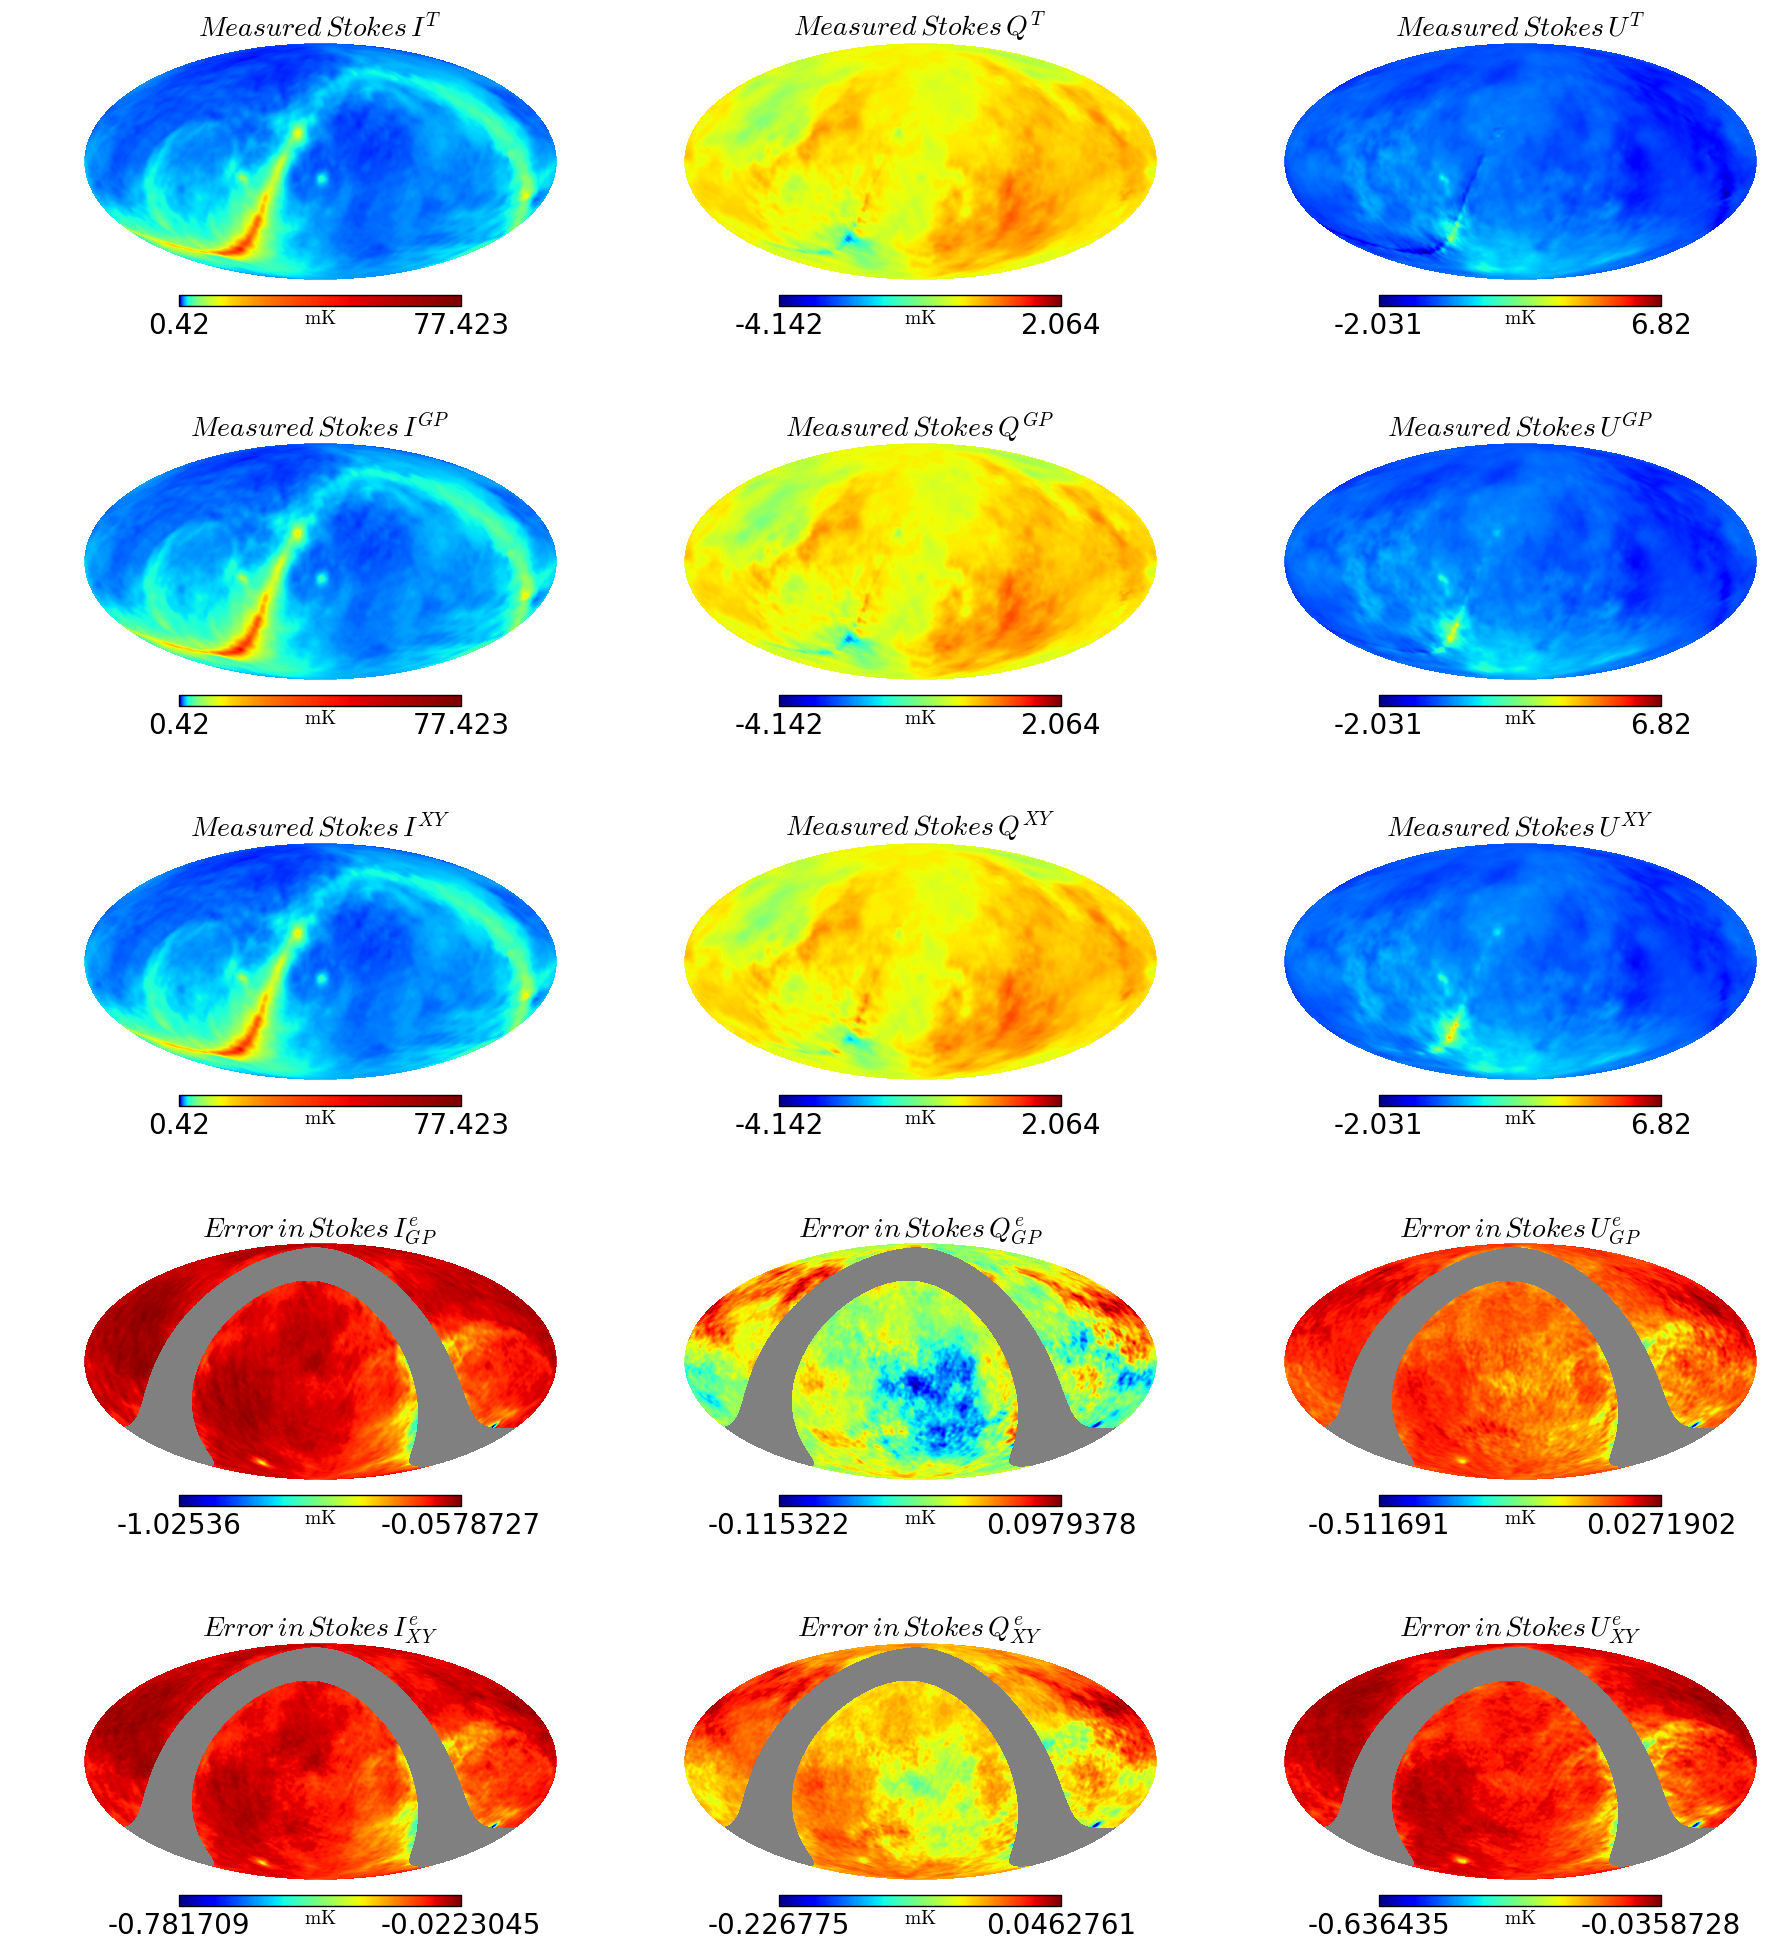
\includegraphics[width=6.6in]{sec3gp_conv/osk_ALL1}
    \end{minipage}
     \caption{The 1\textsuperscript{st} row maps depict the measured foregrounds of Stokes $I$, $Q$ and $U$ for using the non-distorted fully polarised beams in 
     Fig.~\ref{fig:truosk1} whilst the 2\textsuperscript{nd} and 3\textsuperscript{rd} rows represent the corrupted measured foregrounds due to gain and phase and dipole 
     orientation errors introduced into the beams respectively. The next two maps are the corresponding errors in $I$, $Q$ and $U$.}\label{fig:fgGP}
    \end{figure}
    \FloatBarrier
    %%    
The auto-power spectra presented in Fig.~\ref{fig:fg15} estimate the density of the measured foregrounds at different multipole moments. The first three rows in column $1$ show the respective power spectra plots of Stokes I, Q, U when we convolve the polarised foreground with true and gain and phase error beams produced from OSKAR. The next three rows in column $2$ represent the power spectra plots of Stokes I, Q, U respectively when we convolve the polarised foreground with true and dipole position error beams also produced from OSKAR. The last rows in the third column depict the respective power spectra plots of Stokes I, Q, U when we convolve the polarised foreground with two station beams of the JVLA. Note how the beam power in each plot of both OSKAR and the holographic measured beams is normalised to $1$. It is computed by finding the quotient of the power spectrum of the convolved sky map and the original sky map. In addition, note also in all cases, the PB effect of the convolved power spectrum.
The OSKAR beam power plots in Stokes $I$, $Q$ and $U$, converge at a multipole moment of $l=60$.
This value relates to an angular scale of $3.0^\circ$ on the sky whilst the power spectra of the VLA beams converge just at a multipole moment of $l=90$, giving an
angular scale of $2.0^\circ$ on the sky. The change in the value of multipole moments is because of different dish sizes which also results in producing different beamwidths. 
Furthermore, the angular scales computed are equivalent to the beam sizes used to convolve the original maps in Fig.~\ref{fig:f1000}. 
Note, even though we used two different aperture sizes for the simulation, the effect of these two PBs on the convolved power spectra of Stokes $I$, $Q$ and $U$ 
remains unaltered. This shows that in IM experiment, where we  measure the collective emission from many sources, smaller and relatively cheaper instruments can be used.
In this study, the measured values for the convolved power spectra of Stokes $I$, $Q$ and $U$ in both cases are $10\, \mathrm{mK^2}$, $0.1\, \mathrm{mK^2}$ 
and $0.1\, \mathrm{mK^2}$ respectively. Observe carefully how these values in Fig.~\ref{fig:fg15} actually predicted the foreground's temperature of the true sky.
Hence, the power spectrum of the corresponding errors in $I$, $Q$ and $U$ due to perturbation of the beams are $\approx$ $0.01\, \mathrm{mK^2}$, $10^{-4}\, \mathrm{mK^2}$ 
and $10^{-5}\, \mathrm{mK^2}$ respectively.
%%
%% I
  \begin{figure}
      \centering      
      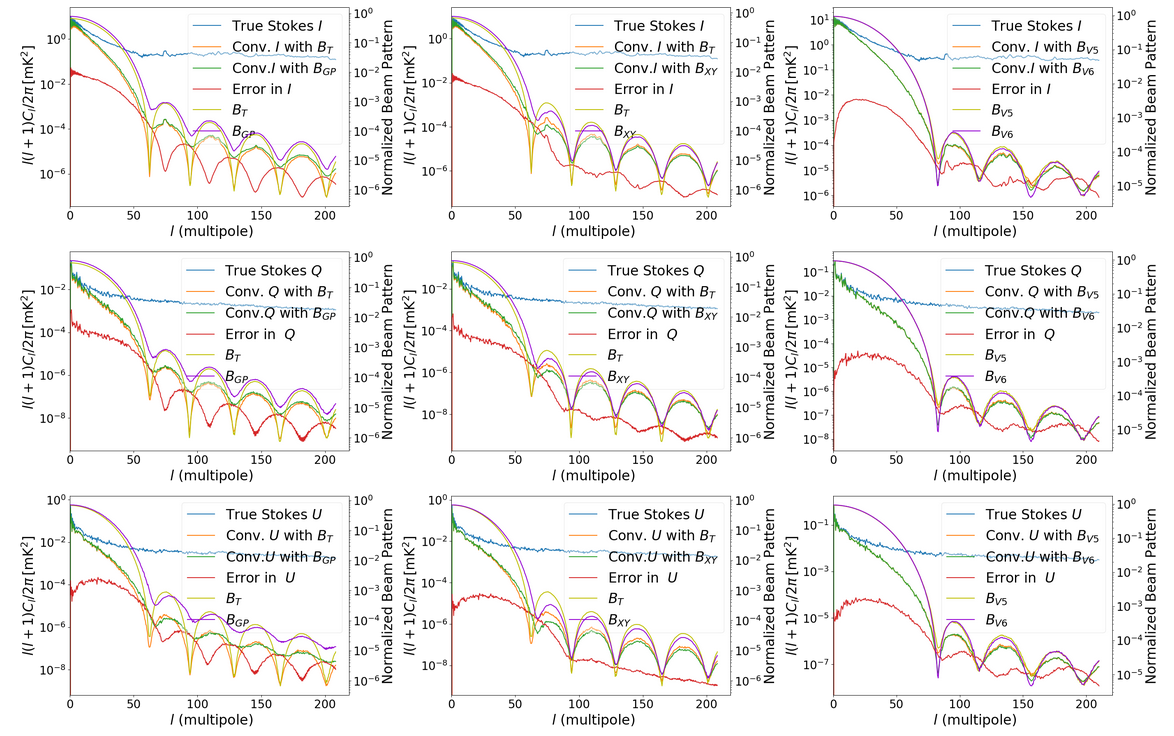
\includegraphics[width=6.8in]{powspectrum/fuck2}    
     \caption{Convolved angular power spectra  estimation of foreground maps. First row: Shows Stokes $I$ spectra plots for using simulated beams and holography measured beams. Second row: Displays Stokes $Q$ spectra plots for using simulated beams and holography measured beams. 
         Third row: Displays Stokes $U$ spectra plots for using simulated beams and holography measured beams.
          }\label{fig:fg15}   
    \end{figure}
    \FloatBarrier
 
% In either case, given the strength of the foregrounds in the galactic 
% centre we will not be able to recover scales less than that (i.e., $l<25$).
%%

% Next, we evaluate the systematic effects of beam errors in Stokes $I$, $Q$ and $U$. 
% 
% We then compute the standard errors of these residual plots to estimate the uncertainties in the angular power spectra when.
The spectra plots in Fig.~\ref{fig:sperr} depict the systematic effects of beam errors in Stokes $I$, $Q$ and $U$. These residual plots are measured as a result of the respective differences between the perturbed and true  measured full-sky maps. From the plots we can clearly observe that the systematic effects of beam errors between the simulated modelled beams and the holographic measurements   differ by 2 or 3 orders of mangitude with respect to the multipole moment ($l$). This is due to the uncertainties introduced in the power spectrum estimation for considering a notional beam over a measured beam.

Table~\ref{tbl:excel-table} shows the corresponding inaccuracies in the power spectrum estimation of Stokes $I$, $Q$ and $U$. It is computed as the standard deviations of the sampling distributions of the residual maps. Here, the residuals are determined as a result of the respective differences between the distorted and non-distorted convolved full-sky maps as reported in Fig.~\ref{fig:fgerr}. This is repeated for the systematic error maps (of using the JVLA holography beams) in Fig.~\ref{fig:B1}. For instance, the standard errors introduced in $Q \longrightarrow I$ are $\approx 0.015$ (due to gain and phase errors) and $0.014$ (due to the main dish surface orientation errors). Also, that of $U \longrightarrow I$ are $\approx 0.005$  and $0.0045$ accordingly. 
% These errors are then used to estimate the imperfections in the simulation by 
% The uncertainties in the spectra plots are as a result of the inaccuracies on the surface of the modelled dish presented in Fig.~\ref{fig:err}.
%%


    %%
 \begin{figure}
\begin{minipage}[H]{\linewidth}
      \centering
      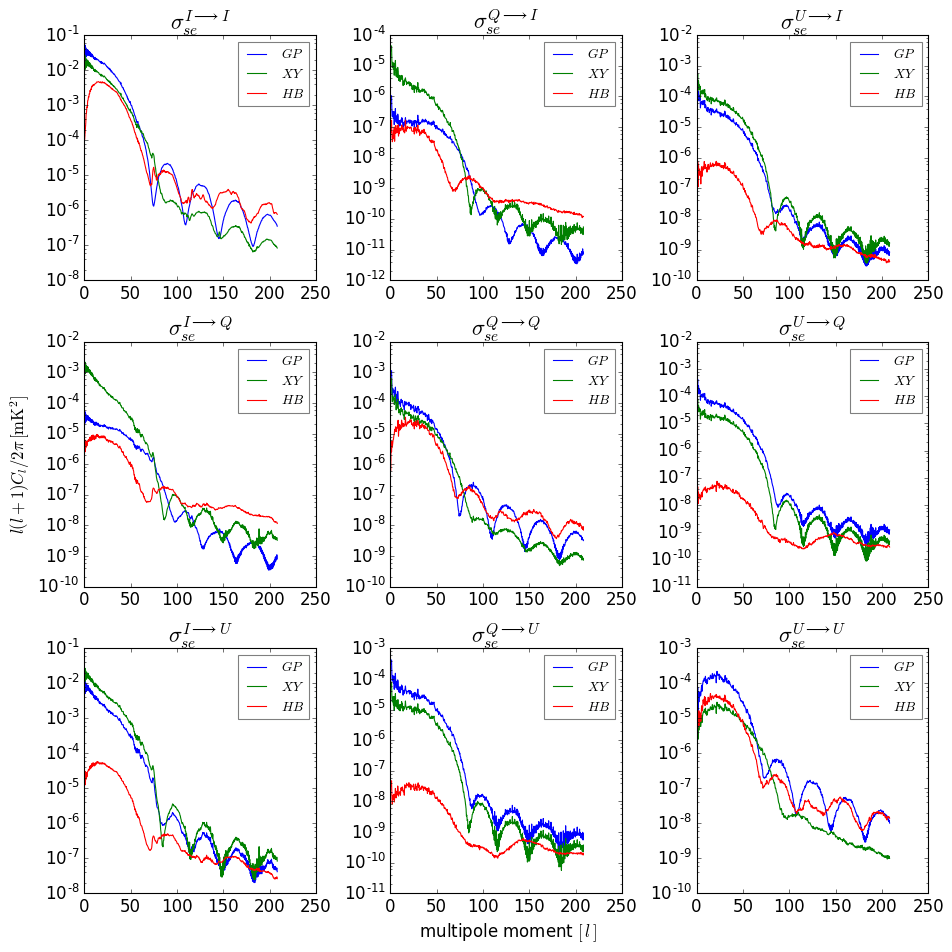
\includegraphics[width=6.6in]{powspectrum/osk_errplots}
      \end{minipage}
    \caption{These are the spectra plots of the systematic errors as shown in Fig.~\ref{fig:fgerr}. 
   The notations $GP$ and $XY$ in the legends denote the residuals for gain-phase and surface orientation errors in the simulated modelled beams, that of $HB$ depicts the errors  in the holography beams. These errors are then used to estimate the imperfections in the simulation by computing the expected value of the standard deviations of the sampling distributions of the residual maps to produce Table~\ref{tbl:excel-table}.}\label{fig:sperr}
\end{figure}
\FloatBarrier
% 
\begin{table}[H]\centering
\caption{Error introduced in the power spectrum estimation} 
\label{tbl:excel-table}
% \ra{1.1}
\begin{tabular}{@{}rrrcrrcrrcrr@{}}\toprule
& \multicolumn{2}{c}{$\bm{I}$} & \phantom{abc}& \multicolumn{2}{c}{$\bm{Q}$} & \phantom{abc} & \multicolumn{2}{c}{$\bm{U}$} & \phantom{abc} & \multicolumn{2}{c}{$\bm{TOTAL}$}\\
\cmidrule{2-3}  \cmidrule{5-6} \cmidrule{8-9} \cmidrule{11-12}
 & $GP $ & $XY $ && $GP$ & $XY $  && $GP $ & $XY $  && $GP$ & $XY $ \\ \midrule
% & GP $ & $ XY $ && $ GP  $ & $ XY $  && $ GP $ & $ XY $  && $ GP $ & $ XY $ \\ \midrule
{}\\
$\bm{I}$ & 0.0640 & 0.0640 && 0.0151 & 0.0137  && 0.0050 & 0.0045 && \textbf{0.0841} & \textbf{0.0822}\\
$\bm{Q}$ & 0.0010 & 0.0008 && 0.0221 & 0.0224 && 0.0007 & 0.0055 && \textbf{0.0238} & \textbf{0.0287}\\
$\bm{U}$ & 0.0007 & 0.0007 && 0.0194 & 0.0341 && 0.0354 & 0.0362  && \textbf{0.0555} & \textbf{0.0710}\\
\bottomrule
\end{tabular}
%\caption{Caption}
\end{table}
 \FloatBarrier     

In IM experiments, the HI signal is measured in Stokes $I$, so we are particularly interested in the total intensity and the leakages from polarization 
into Stokes $I$ (that is, $|Q + iU| \longrightarrow I$). Fig.~\ref{fig:lk} shows how the $|Q + iU| \longrightarrow I$  and the error in Stokes $I$ map affect the HI signal. 
Here, a spherical power spectrum of the simulated model of $21\, \mathrm{cm}$  brightness temperature at $z \approx 0.67$ produced from the 
CRIME\footnote{{\tt http://intensitymapping.physics.ox.ac.uk/CRIME.html}} fast simulation software and described by \citep{2014MNRAS.444.3183A} 
is generated and then compared with the spectra plots of the  Galactic foregrounds. % presented in Figs.~\ref{fig:lk1} and~\ref{fig:lk2}. 
The HI signal power in the right side of the plot is higher than the $|Q + iU| \longrightarrow I$ at a multipole moment of $l=100$ which is about $4$ orders of magnitude greater at lower scales. 
This occurs when we do not correct the beam errors (i.e., gain, phase and orientation) in Stokes $I$ at all. 
The fractional leakage of $|Q + iU|/I$ is computed to give $\approx 1.0 \%$ for the intrinsic case (i.e., $|Q + iU|_{\rm T}$) where a true model of the beam is known.
The spectra plots reported in the other plot, try to correct the columns that feeds into Stokes $I$ (i.e., $Q \longrightarrow I$, $U \longrightarrow I$ and $I \longrightarrow I$)
by assuming the corresponding beams (i.e., $m_{\rm QI}$, $m_{\rm UI}$ and $m_{\rm II}$) are not known to the extent to which they have been assumed in this paper. In this case,
the power spectrum of the HI signal can be observed at a multipole moment of $l=25$.
We conclude that if the knowledge of the beam is of a similar quality than the one assumed in this paper, then we will be able to recover the cosmological HI signal 
without great problems and without further calibration on scales larger than $l = 100$. However, this work suggests that if polarization calibration is performed correctly 
then results can be improved and we can recover scales above $l=25$. 
%%
\begin{figure}
\centering    
    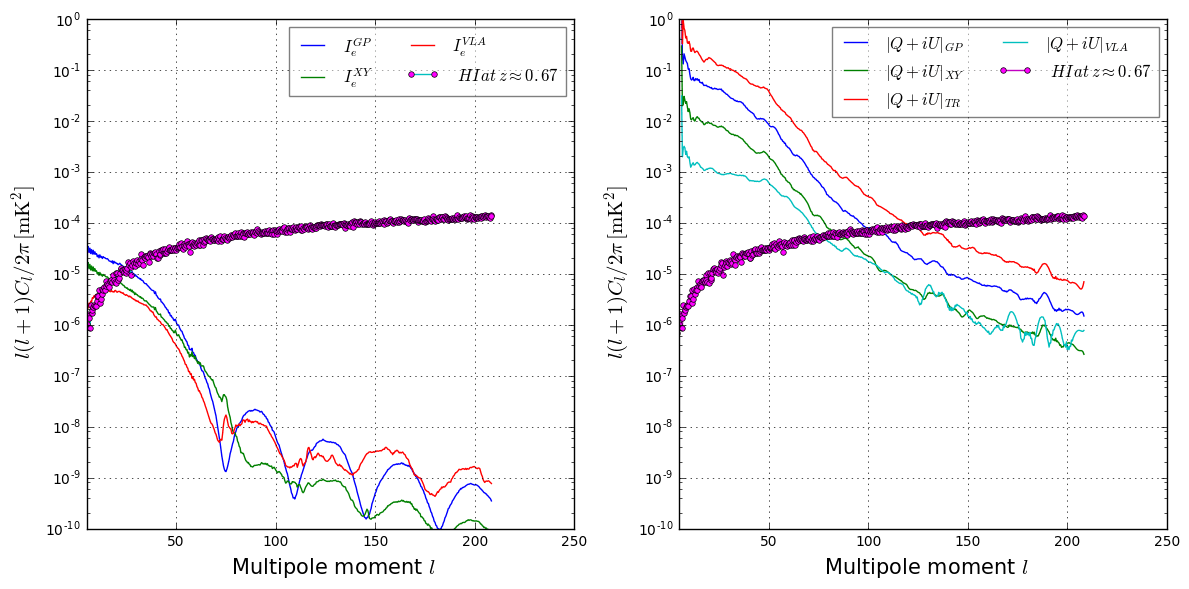
\includegraphics[width=\linewidth]{powspectrum/hisim}
 \caption{The spectra plots compare the effect of recovering the cosmological $21\, \mathrm{cm}$ signal by calibrating for the beam errors in Stokes $I$ 
  to when there is no beam correction at  all. The solid circular spectrum is the simulated $21\, \mathrm{cm}$ 
  brightness temperature described by \citep{2014MNRAS.444.3183A} at a $z\approx 0.67$. 
  LEFT SIDE PLOT: Here, we show how to estimate the $21\, \mathrm{cm}$ signal when we correct the errors in Stokes $I$.         
  RIGHT SIDE PLOT: We quantify the amount of leakages into Stokes $I$ when we do not perform any beam correction.
  The spectrum $ (|Q + iU|_{T} )$, is the intrinsic leakage in $I$ when we adopt true modelled beams as shown in  Fig.~\ref{fig:truosk1}.
  The other plots $( |Q + iU|_{GP}, |Q + iU|_{XY} , |Q + iU|_{VLA})$  are the leakages in $I$ when we use perturbed modelled beams (i.e., gain, phase and main dish surface orientation errors) and holography measured beams respectively.}\label{fig:lk}
 \end{figure} 
 \FloatBarrier

 
%     
\section{Conclusions} \label{sec:conclusions}
%%
The study introduces an application of the OSKAR software as a relatively cheap technique to produce realistic PBs and perturbations
(using gain, phase, and main dish surface orientation errors) for IM experiments. These fully polarized modelled beams are then
used to simulate the full-sky polarization maps by the method of convolution in order to compute the intensities of the diffuse
Galactic foregrounds and determine the amount of signal that has seeped from linear polarization into total intensity. The simulation is
repeated using the holography-measured beams and then compared with the modelled beams in order to estimate the error introduced in
the power spectrum when modelled beams are used. The following are the key findings of the research:

\begin{itemize}
\item We use $80 000$ dipoles to model the distribution of the dish-like surface of the antenna. This produces $\approx 0.10$ per cent perturbed
inaccuracies on the dish surface due to the random placement of the dipoles, which are not exactly phased up. The value of the perturbed
inaccuracies will increase if the number of dipoles is $\ll 80 000$.
%%
\item The perturbed inaccuracies due to the imperfections in the nominal orientation of the dipoles introduce fractional errors of
$0.08 \%$ for Stokes $I$, $0.03 \%$ for $Q$ and $0.07 \%$ for $U$ in the convolved power spectrum estimation. 
Note that these occur when we assume to use modelled beams whilst we convolve the foregrounds with measured beams.
%%
\item Furthermore, if we construct a model of a beam and then carry out polarization rotation and calibration of the phase in order
to correct the beam in Stokes $I$, then the power of the HI signal can be estimated at a multipole moment of $l = 25$. But, if we don’t do
any correction at all for the beam, then the power spectrum of the HI signal is measured at a multipole moment of $l=100$. This makes
the latter multipole moment be $\approx 4$ orders of magnitude higher than when we correct the error in the beam.

\item Finally, if a true model of the beam is assumed, then the intrinsic fractional leakage of $|Q + iU|_{\rm T} \longrightarrow I$ is $\approx 1.0$ percent.
\end{itemize}
%%
\noindent  To recap, we have shown that the {\tt oskar} package can simulate the beam patterns and as well as distortions of the dish. The model we adopted to do this, is to 
create a dense set of dipole orientations that imitate the aperture illumination patterns of the dish, with full blockage from the quad leg structure and other supporting frame.
The convolution technique has shown to be a good mathematical model to use for measuring the intensity of the foreground. Hence, for a full polarization model 
of the beams, we can  actually measure the fractional leakages we are instereted in. For the next chapter, we extend this simulation technique to investigate HI intensity mapping 
with MeerKAT L-band beams. 
%%

%%
\chapter{MeerKAT L-Band Primary Beams: Effects of HI Intensity Mapping} \label{Chapter5} 
%% Main chapter title

 % For referencing the chapter elsewhere, use \ref{Chapter1} 

\textbf{Overview}\\
% \HRule \\[0.4cm]
\par\noindent\rule{\textwidth}{0.4pt}\\
\textit{This chapter introduces us to the Zernike model and how it can be used to reconstruct a realistic beam model using
the strongest coefficients (selected number of Zernike coefficients) with corresponding basis patterns. An intensity mapping experiment is performed with these
primary beams to evaluate the angular power spectrum of 21 cm signal.
}%\\
% \HRule \\[1.5cm]
\par\noindent\rule{\textwidth}{0.4pt}
%%

\noindent \texttt{Author’s comment:} 
\small{The primary beam model used in this chapter is part of the work in: K. M. B. Asad, J. N. Girard, M. de Villiers, \textbf{T. Ansah-Narh}, K. Iheanetu, O. Smirnov, M. G. Santos, and others, Primary Beam Effects of Radio Astronomy Antennas – II. Modelling the MeerKAT L-band Beam using Holography. The Monthly Notices of the Royal Astronomical Society (MNRAS), accepted. We therefore confirm that part of the wording in this chapter will  “match” that of the paper. Hence, this note serves as a universal reference for all such text.}

%%
\section{Introduction}	   \label{chap5:intro}
%%

The completely operational MeerKAT instrument is situated in Karoo (a desert area) of South Africa and, is  made up of $64$ \enquote*{offset Gregorian} interferometer. The measurement across the main dish is $13.5 \, \rm m$, that of the secondary reflector is $3.8 \, \rm m$  and, has a maximum separation of $8\, \rm km$.
Almost $70\%$ of the receptors are found in the core area of $1 \, \rm km$ in width. The central location of the interferometer is at latitude $-30\rm d42\rm m47.41\rm s$ and longitude $21\rm d26\rm m38.00\rm s$. There are four feeds on each receptor with the L-band having a frequency range of $0.9 - 1.67\, \rm GHz$.
It also has digitisers supported on the feed indexer. The offset design of MeerKAT provides a better aperture efficiency, a symmetric beam pattern with a decrease in the side-lobes and an increase in the antenna gain. 
The relatively small diameter of the MeerKAT antennas coupled with the large number of antennas and large total collecting makes it a powerful wide-field imaging instrument, with a combination of large field-of-view, wide-bandwidth, high sensitivity and outstanding sampling of the Fourier transform of the sky with 2016 instantaneous baseline samples.

Fig.~\ref{fig:meerkat_layout} displays the station layout of the MeerKAT elements with the left panel showing the representation of the outermost layout and  that of the right panel showing the innermost layout. 
\noindent Refer to \citep{jonas2018meerkat,2018PhyW...31h...8M,2018SPIE10704E..1UR,Santos:2017qgq,taylor2017mightee} for further reading on the design of MeerKAT and its capabilities for science research.

%
%	+++++++++++++++++++++++++++++++++++++++++++
%	MeerKAT Layout
%	++++++++++++++++++++++++++++++++++++++++++++
%
\begin{figure}[ht]
    \centering	    
    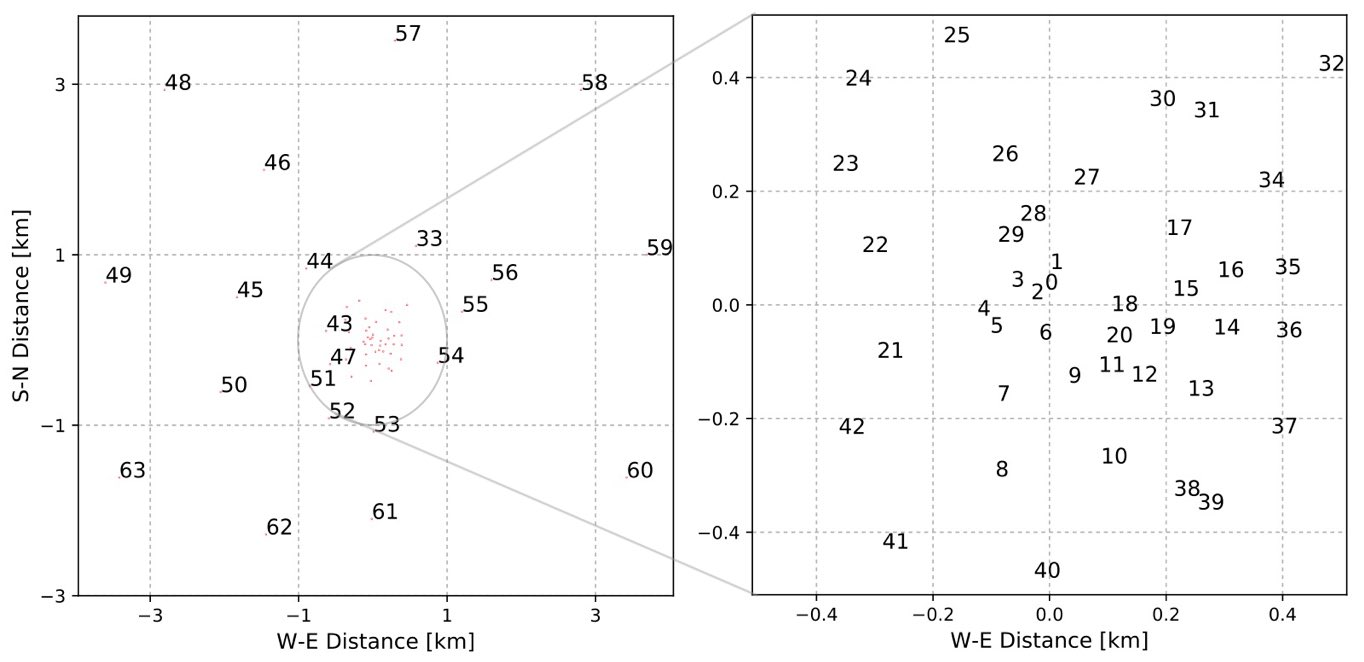
\includegraphics[width=5.8in]{c5/meerkat_layoutt}	    	   
    \caption{The distribution of the 64 antennas of MeerKAT, each identified by an integer ranging from 0 to 63. Note that the actual names of the antennas are given as M000, M001, M002 and so on. Left: The distribution outside the 1 km core. Right: The distribution inside the 1 km  core is loosely delimited by a hexagonal boundary. The West-East and South-North distances are shown relative to the arbitrary centre located at −30d42m47.41s South, 21d26m38.00s East.}
	    \label{fig:meerkat_layout}
       \end{figure}
  \FloatBarrier 
%%

 \begin{figure}[ht]
	    \centering	    
	    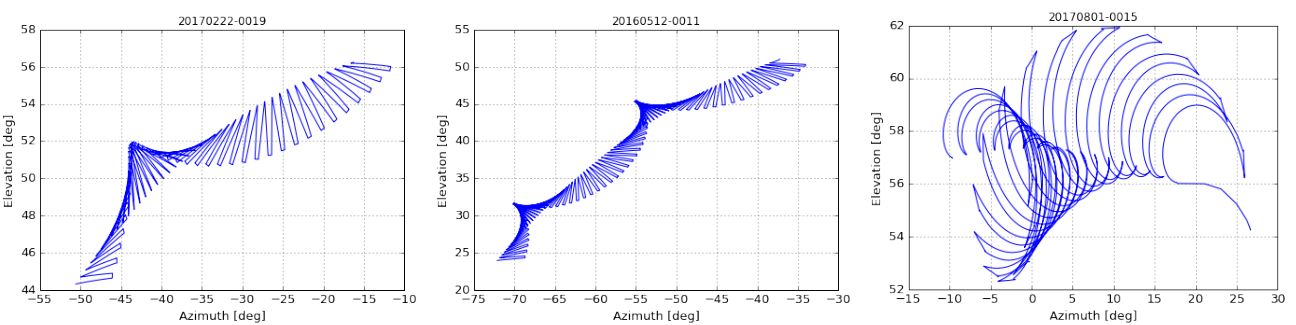
\includegraphics[width=6.2in]{c5/nn} %rasterscnn
	    %\vspace{5 mm}	   
	    \caption{The raster scanning patterns of three of the astro-holographic observations of MeerKAT. The title indicates the observation
ID. More information about the observations can be found in Table 1 and inside the text.}
	    \label{fig:rasterscn}
       \end{figure}
  \FloatBarrier 
% 

One major technique used in radio interferometry in order to measure the complex beam pattern of an antenna, is the holography. Generally, to produce a holography beam model, one radio telescope points constantly at a cosmic radio source whilst another telescope drifts across the source, usually in a raster scan form. We then obtain the complex beam pattern in terms of amplitude and phase by correlating the respective output powers with the reference antenna pointing at the same source. 

The main target source observed in this work is 3C 273 at a frequency of $1.365 \, \rm GHz$. In addition, Fig.~\ref{fig:rasterscn}  shows the patterns of the various raster scans used in this study. The 2017-02-22 observation was performed using three scanning antennas (M000, M012, M017) and one tracking antenna (M011). The scanning and tracking were performed from an elevation angle of $44^{\circ} \sim 57^{\circ}$, as seen in the figure, but we can also see that the beam is well-sampled within only a circular region of around $\sim 6^{\circ}$ diameter, centred at an elevation of $51.08^{\circ}$. The centre elevation is obtained from the average of the tracked elevations.
%
\noindent The holographic measurement of this radio interferometer is discussed extensively in  \citep{7305152}. Here, the observation is done not directly using the traditional raster scan approach as presented in \citep{1988A&A...190..353E} but instead, a complex scanning pattern like the one displayed in Fig.~\ref{fig:rasterscn}. This method is efficient because it cuts out the need for slew scans in the traditional way, and hence reduces the tracking period. However, the complex beams produced from this scheme are perturbed with undesirable radio frequency interference (RFI). The source of this disturbing noise can be resolving satellites and other physical radio emissions. Therefore, it is necessary to introduce a mathematical model to reconstruct these holography measured beams which is the main objective of this research, in order to denoise the data and achieve a high accuracy. In the original paper, we demonstrated three different numerical techniques namely; modified-Principal Component Analysis (PCA), Spherical Harmonics (SH) and Zernike Moment (ZM) to model the measured beams. For the purpose of this study, we focus on ZM only. Here, we want to further explore how the IM techniques discussed in Chapter~\ref{Chapter4} scale  to MeerKAT telescopes. Thus, instead of using {\tt OSKAR} to simulate perturbed fully polarized beams, we fit Zernike polynomials to MeerKAT holography measured beams using a particular number of Zernike coefficients with corresponding basis functions and then perturb the beams with the fit again, using different number of coefficients. We then simulate these reconstructed beams with the foregrounds to determine the leakage terms. 

The mathematical function of ZMs was originally developed to tactle wavefronts in optics. Now, the model has been adopted in many applications of image analysis such as image reconstruction~\citep{6243926}, image classification~\citep{1414392,khotanzad1990classification}, and image retrieval~\citep{7569541}. The orthogonal property of ZMs can depict an image with arbitrary number of polynomilas using the highest coefficients~\citep{teh1988image}. 

Next we present the mathematical model of ZM.
% Note, One of the MeerKAT beam models presented here is available through the openly accessible package EIDOS. 
%  the effects of the beam on HI intensity mapping 
 


\section{Methodology}	   \label{chap5:mkbeams}
%%

\subsection{Mathematical Basis of Zernike Polynomials}	   \label{chap5:zernike}
%%


Consider a wavefront  denoted by $\Phi_{w}(\rho,\theta)$, in polar coordinates $(\rho,\theta)$, to be a linear combination of Zernike polynomials over a circular unit, then this phenomenon can mathematically be expressed as:
\begin{equation}
 \Phi_{w}(\rho,\theta) = \sum\limits_{\rm \beta, \rm \alpha}^{M} C_{\rm \beta}^{\rm \alpha}Z_{\rm \beta}^{\rm \alpha}(\rho,\theta) %\sum\limits_{m = 0}^{n}
  \label{eq:wavefront}
\end{equation}
%

\noindent The \textit{basis of ZM} $Z_{\rm \beta}^{\rm \alpha}(\rho,\theta)$, in Equation~\ref{eq:wavefront} is defined as \citep{2015arXiv150607396F}: 
 
 \begin{equation}  \label{eq:zm}
Z_{\rm \beta}^{\rm \alpha}(\rho,\theta) = \left\{ \begin{array}{cc} 
                \Lambda_{\rm \beta}^{\rm \alpha} R_{\rm \beta}^{\lvert \rm \alpha \rvert}(\rho) \cos(\rho \rm \alpha \theta), & \hspace{3mm} \rm \alpha \geq 0 \\
                -\Lambda_{\rm \beta}^{\rm \alpha} R_{\rm \beta}^{\lvert \rm \alpha \rvert}(\rho) \sin(\rho \rm \alpha \theta), & \hspace{3mm} \rm \alpha < 0\\                
                \end{array} \right.
\end{equation}

\noindent The \textit{radial polynomial} $R_{\rm \beta}^{\lvert \rm \alpha \rvert}(\rho)$ and the \textit{normalisation factor} $\Lambda_{\rm \beta}^{\rm \alpha}$ in Equation~\ref{eq:zm} are respectively denoted as:\\

$R_{\rm \beta}^{\lvert \rm \alpha \rvert}(\rho)  = \sum\limits_{s = 0}^{\frac{\rm \beta - \lvert \rm \alpha \rvert}{2}}  \frac{(-1)^{s}(\rm \beta-s)! \rho^{\rm \beta-2s}}{s!\left[\frac{\rm \beta + \lvert \rm \alpha \rvert}{2} -s\right]!\left[\frac{\rm \beta - \lvert \rm \alpha \rvert}{2} -s\right]!}$, \quad 
$\Lambda_{\rm \beta}^{\rm \alpha} = \sqrt{\frac{2\rm \beta+1}{1+\delta_{\rm \alpha,\rm 0}}}$ \\
 
\noindent where $\delta_{\rm \alpha,\rm 0}$ is the Kronecker delta function such that $\delta_{0,0} = 1$ and $\delta_{\rm \alpha,\rm 0} = 0$ when $\rm \alpha \neq 0$.  The index $\rm \beta \geq 0$: $\rm \beta = 0, 1, 2, \ldots $ and 
for a specific $\rm \beta$, the index $\rm \alpha$ takes the values $\rm \alpha = -\rm \beta, -\rm \beta + 2, -\rm \beta + 4,  \ldots , \rm \beta$.
%%

\noindent The polynomials $Z_{\rm \beta}^{\rm \alpha}(\rho,\theta)$ are a set of complete orthogonal over a unit circle and this is conveniently represented in Equation~\ref{eq:zm} as the products of angular functions and radial polynomials. The orthogonality of this function makes the coefficients not to be dependent on one another \citep{charman2005wavefront,wyant1992basic} and hence, these coefficients are normally expressed in double $(\rm \beta, \rm \alpha)$ or single $(j)$ modes. The $\rm \beta$ mode characterises the order of aberration and mode $\rm \alpha$ represents the azimuthal frequency of the sinusoidal. The radius parameter, denoted $\rho$, is continuous over the range of $(0, 1)$ and this means the azimuthal component is continuous over the range of $\theta$, such that $ 0 \leq \theta \leq 2\pi $. Fig.~\ref{fig:rp} displays $8$ of such radial responses, where it can clearly be observed that the polynomials converge as they approach the edge of the unit disc. This also confirms that the Zernike polynomials of all orders are confined to the interval $(-1,1)$ as shown in Fig.~\ref{fig:d_indx}. 
%
% 

\begin{figure}
\begin{minipage}[H]{\linewidth}
      \centering
      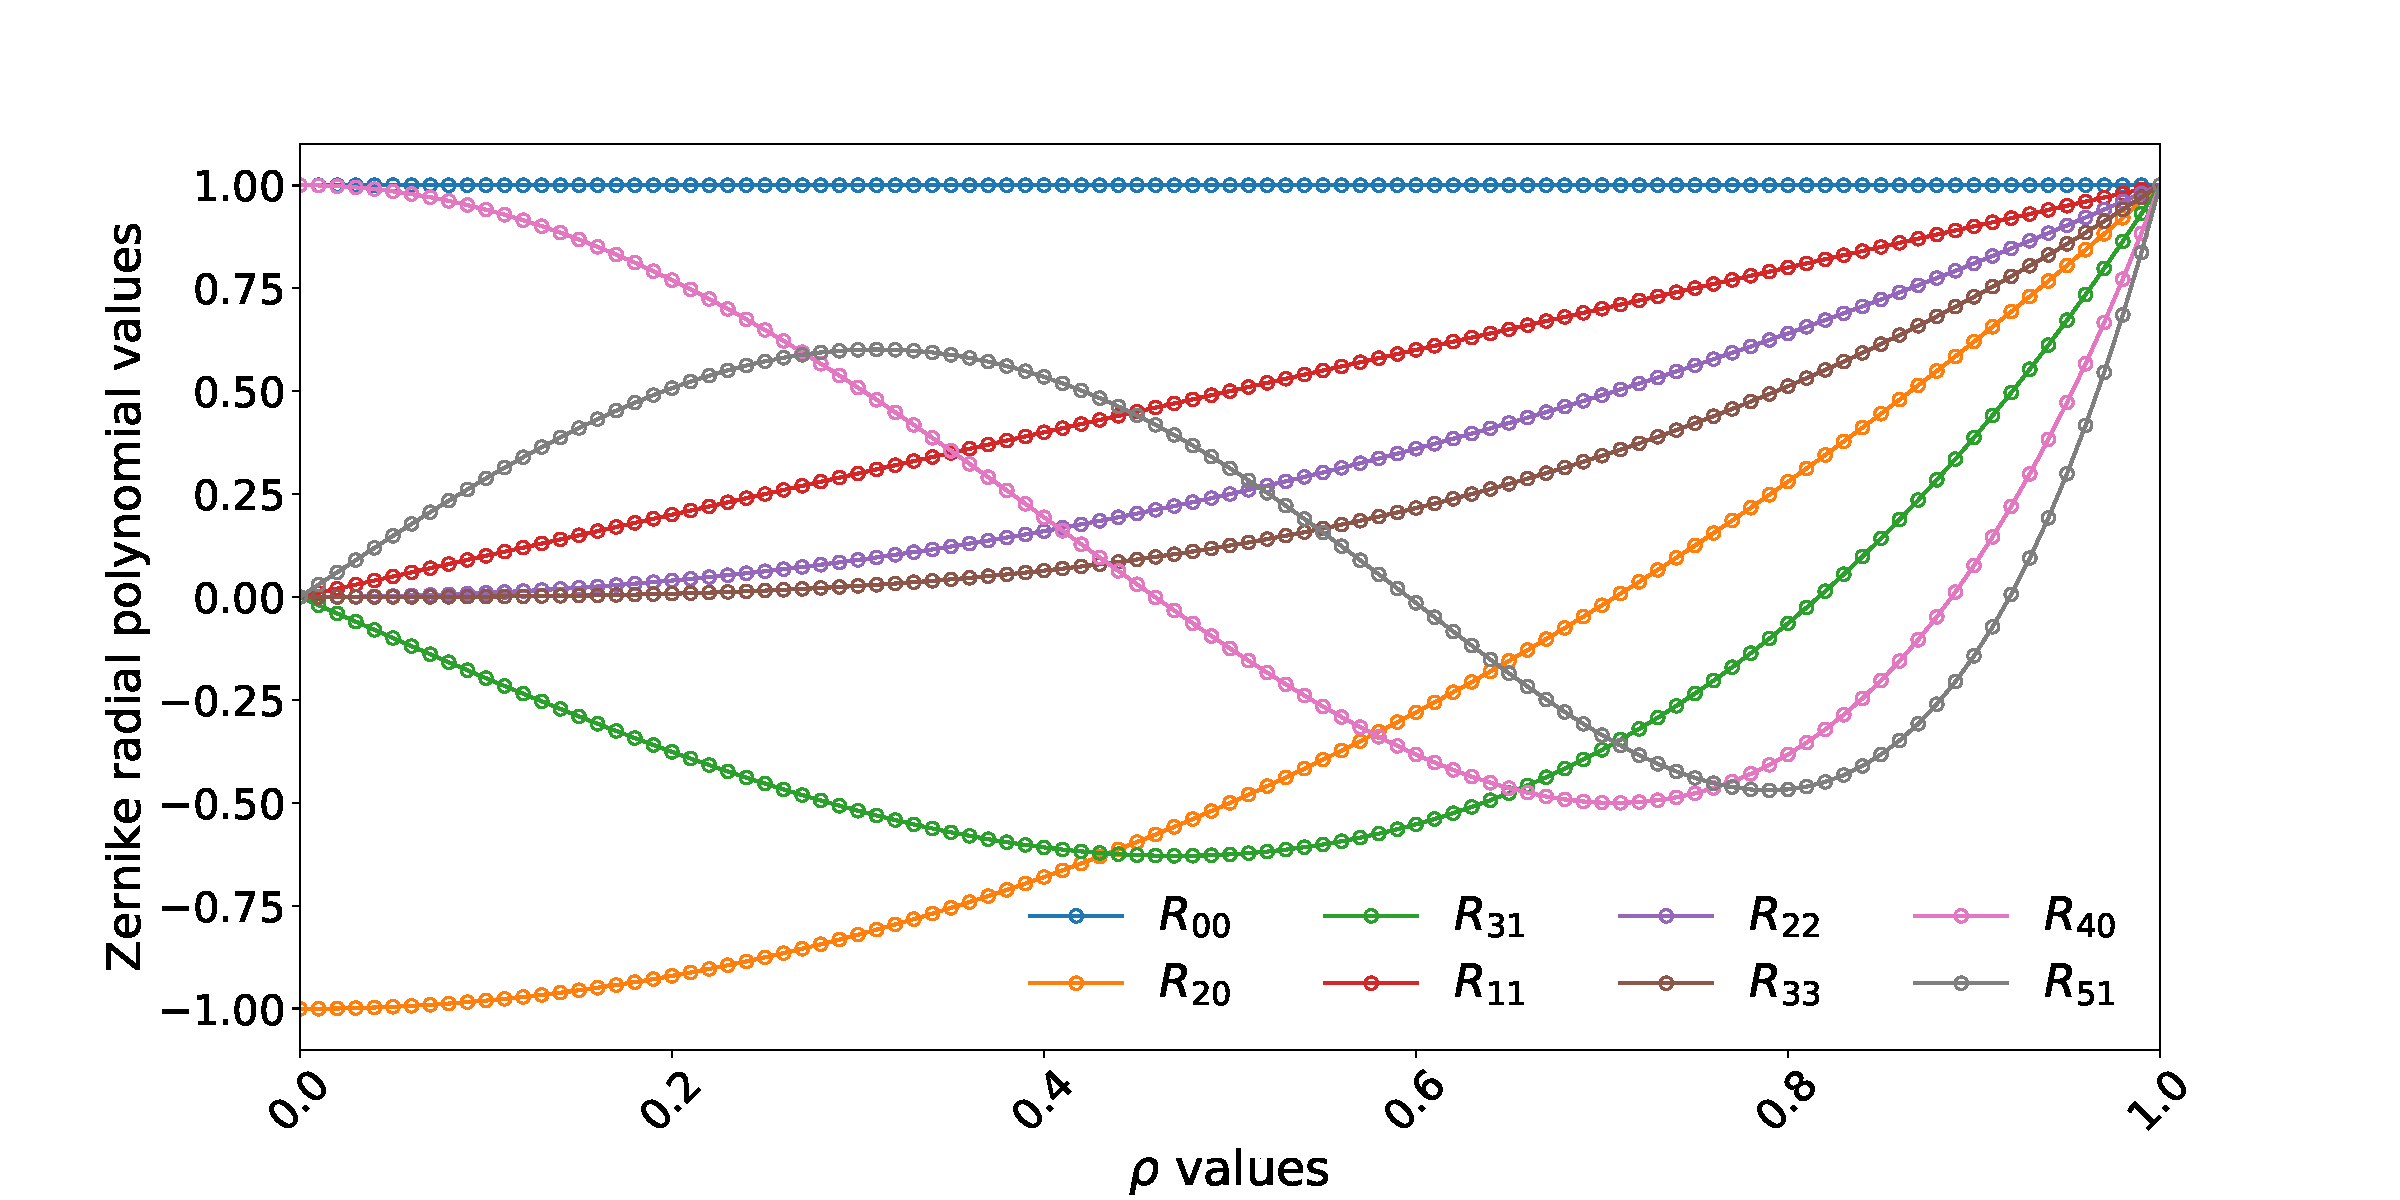
\includegraphics[width=\linewidth]{c5/rad_plot} %6.6in
      \end{minipage}
    \caption{\label{fig:rp} Expansion of eight orthogonal radial polynomial $R_{}^{\lvert \rm \alpha \rvert}(\rho)$ plots. Here, the value of unity can be obtained at the
outer edge, since $R_{\rm \beta}^{\lvert \rm \alpha \rvert}(1) = 1$.}
\end{figure}
\FloatBarrier
%%
%%

The surface plots in Fig.~\ref{fig:d_indx} depict the Zernike pyramid formed by the first $6$ levels. In the central column, the modes are invariant by rotation $(\text{i.e.} \, \rm \alpha=0)$ and hence, the column can be seen as a symmetry around the axis. On each level (i.e. same $\rm \beta$ value), the Zernike modes of opposite azimuthal frequency value have the same overall shape, but a different orientation. These pairs are required to enable any mode to be freely moved around $360^\circ$, by selectively adjusting the weight of each mode to obtain the desired orientation. Note, for further discussions on ZM, we can refer to these articles \citep{campbell2003new,lakshminarayanan2011zernike,1976JOSA...66..207N,wyant1992basic}.
% For further reading on ZM

%%

\begin{figure}
\begin{minipage}[H]{\linewidth}
\centering
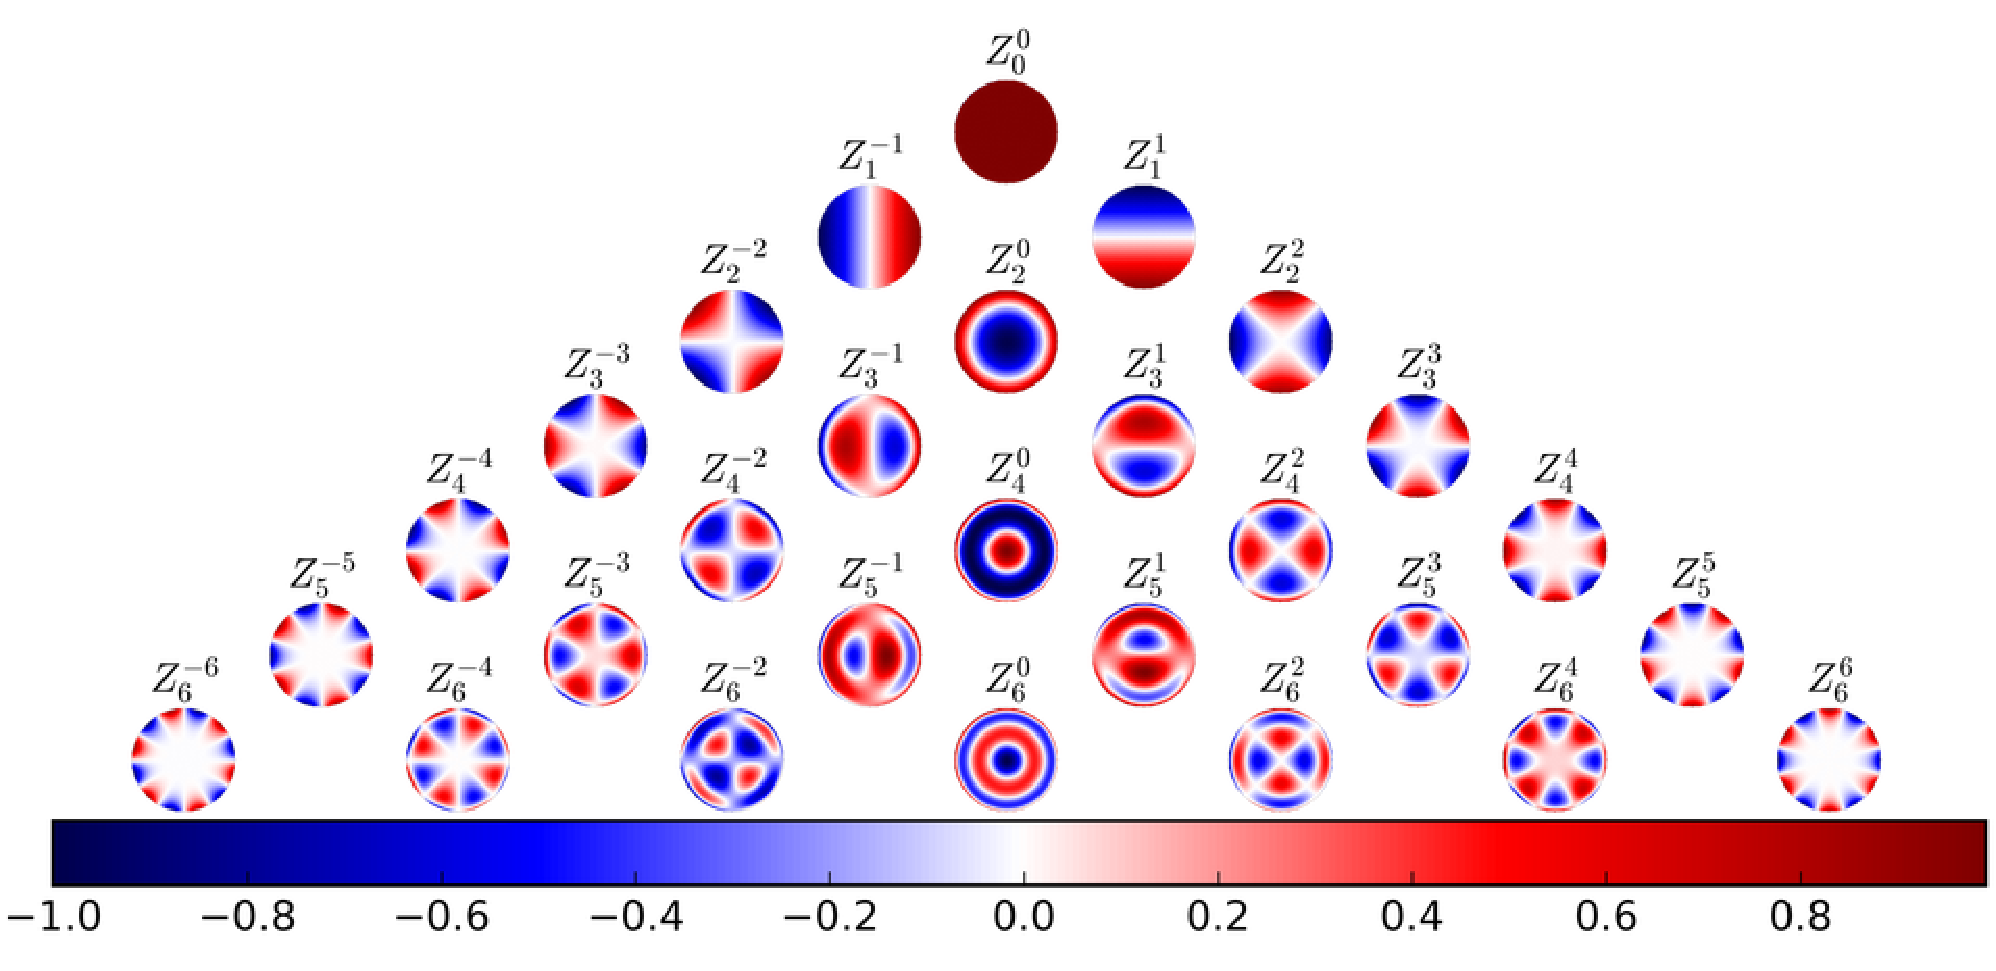
\includegraphics[width=\linewidth]{c5/kelazern}
\end{minipage}
\caption{\label{fig:d_indx} Representation of basis patterns of Zernike moments $Z_{\rm \beta}^{\rm \alpha}(\rho,\theta)$ of order $6$, plotted on a unit circle.}
\end{figure}
\FloatBarrier
%%

% %%
\subsection{Numerical Computation of Zernike Coefficients}	   \label{chap5:zcoff}
%%
In Equation~\ref{eq:wavefront}, the vector variable $C_{\rm \beta}^{\rm \alpha}$ (Zernike coefficient) is the only unknown factor that needs to be computed. 
Let $L$ denote the pixel positions of the measured beam $\Phi_{w}$, such that $\Phi_{w}^{\tau}(\rho_{\tau},\theta_{\tau})\mid_{\tau = 1,2,3,\ldots,L}$, where
$(\rho_{\tau},\theta_{\tau})$ is the corresponding pixel coordinate usually in polar form.  We then estimate the parameter $C_{\rm \beta}^{\rm \alpha}$ 
by rewriting Equation~\ref{eq:wavefront} in a simple form as expressed in Equation~\ref{eq:lsq} and then try to solve the least square problem using 
the matrix inversion approach. 
%%

\begin{equation}\label{eq:lsq}
 \bm{Z}_{\rm P \times L} \bm{C}_{\rm P \times 1} = \bm{\Phi}_{\rm L \times 1}
\end{equation}

\noindent where $\bm{\Phi}$ is the $L \times 1$ data array\footnote{{\tt The package numpy.ravel will return a neighbouring flattened array.}} that consists of  
the MeerKAT beams, $\bm{C}$ is the unknown coefficients of $ P \times 1$ array and  $\bm{Z}$ is the $P \times L$ matrix of polynomials that  provides 
the physical features of $\bm{\Phi}$. Expanding Equation~\ref{eq:lsq} we get;

\begin{equation}
{
 \begin{pmatrix}
   Z_{1}(\rho_{1},\theta_{1}) & Z_{2}(\rho_{1},\theta_{1}) & \cdots & Z_{P}(\rho_{1},\theta_{1})\\
   Z_{1}(\rho_{2},\theta_{2}) & Z_{2}(\rho_{2},\theta_{2}) & \cdots & Z_{P}(\rho_{2},\theta_{2})\\
    \vdots                    &     \vdots                 & \ddots &    \vdots  \\     
   Z_{1}(\rho_{L},\theta_{L}) & Z_{2}(\rho_{L},\theta_{L}) & \cdots & Z_{P}(\rho_{L},\theta_{L})
   \end{pmatrix}  \begin{pmatrix} c_{1}\\
				  c_{2}\\
				  \vdots\\
				  c_{L}
    
   \end{pmatrix} = 
   \begin{pmatrix}
    \Phi(\rho_{1},\theta_{1})\\
    \Phi(\rho_{2},\theta_{2})\\
    \vdots\\
    \Phi(\rho_{L},\theta_{L})\\
    
   \end{pmatrix}
  } \label{eq:lsq1}
  \end{equation}
%%
The resultant equation can be written in the form:

\begin{equation} \label{eq:invmthd}
 \bm{Z^{T}ZC} =  \bm{Z^{T}\Phi}
\end{equation}

\noindent such that, the desired Zernike coefficients can be obtained by direct inversion;

\begin{equation} \label{eq:invmthd2}
 \bm{C} =  \bm{(Z^{T}Z)^{-1}Z^{T}\Phi}
\end{equation}
%%

\noindent Therefore, given the basis patterns of Zernike polynomials and the corresponding coefficients, we can use these to reconstruct a particular wavefront.
In this study, the MeerKAT holography primary beams are used to represent the wavefront and then fit Zernike polynomials to reconstruct the measured beams.


%%%
% \subsection{Image Reconstruction} \label{chap5:img_reconstr}
%%
\subsection{Spatial Representation}	   \label{chap5:spatial}
%%

Note here that we represent the MeerKAT beams in the Jones matrix form as XX\footnote{{\tt Horizontal linearly unpolarized beam}}, XY\footnote{{\tt Horizontal linearly polarized beam}}, YX\footnote{{\tt Vertical linearly polarized beam }}, YY\footnote{{\tt Vertical linearly unpolarized beam}}. Therefore, these notations have the same meaning through out this chapter.

In this work, we select the strongest coefficient values to denoise the MeerKAT beams at $990\, \mathrm{MHz}$. The selection is done base on the modal number with a reduced value of root mean square deviation (RMSD: $[ 1/N \sum\limits_{k=1}^{N} \parallel \bm{D}_{\rm k}^{a} - \bm{D}_{\rm k}^{e}\parallel^{2}]^{1/2}$ where $N$ is the beam size, $\bm{D}_{\rm k}^{e}$ is the Zernike fitted beam and $\bm{D}_{\rm k}^{a}$ is the original beam) as reported in Fig.~\ref{fig:beams_mse}. The RMSD plots of XX and YY in Fig.~\ref{fig:beams_mse} (blue and red) show that, we can use $20$ strongest angular frequencies (m-modes) with $RSMD \approx 0.001$ to model the gain part of the original holography beams, since increasing the number of m-modes will not significantly improve the reconstructed model. The same explanation goes to the cross term plots (yellow and green), where we choose the $5$ strongest modes with $RSMD \approx 0.001$ and the respective coefficients to reconstruct.

The principal idea to adopt the Zernike scheme in this study is to decrease the number of feature parameters (i.e. Zernike basis functions)
required to depict the spatial morphology since generally, Zernike coefficients are highly sparse. If we use a smaller number of coefficients, there's the possibility that the modelled image  will not be well-fitted. In addition, if the number of coefficients is very high, there's the likelihood of over-fitting the modelled image. In this research, we cautiously choose the strongest number of coefficients by truncating the coefficients up to a given threshold parameter based on the RMSD value.
%%
%%
\begin{figure}
\begin{minipage}[H]{\linewidth}
\centering
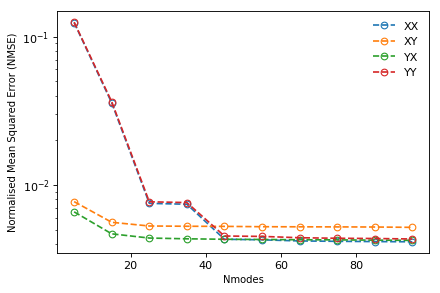
\includegraphics[width=\linewidth]{c5/mse_err3} %mkk/mse}
\caption{\label{fig:beams_mse} The expected value of the squared error loss  between the holography beam and the predicted beam model with respect to 
increase in the number of Zernike modes. (XX, YY) and  (XY,YX) are the linear polarization for the gain and cross terms of the Jones beams respectively.}
\end{minipage}
\end{figure}
\FloatBarrier
%%
We use this idea to reconstruct a 2D image from a Zernike fit. Here, all we need to have are the coefficients and the respective basis functions.
Fig.~\ref{fig:b20-5} shows a reconstructed MeerKAT beam model at a frequency of $990$ MHz for antenna M017. Note how the Zernike modelled beams (middle plots)
have de-noised the original beams. To test the goodness of fit of this model, we vary the number of Zernike coefficients and compare their residuals. The 1st $2$ plots in Fig.~\ref{fig:3rad} are the radial profile plots 
when we use the $5$ strongest coefficients for all the Jones terms and the $10$ strongest coefficients for all the Jones terms respectively. 
Note how the standard errors of these plots are higher than the 3rd plots which occur when we use the coefficients of $20$ and $5$  for the gain and cross terms respectively. This is confirmed when we also look at the distribution of the histogram plots in Fig.~\ref{fig:3hist}. Using $>5$ strongest coefficients to model the cross terms and  $<20$ strongest coefficients to model the gain terms will result in the perturbation of the beams. 

% 
%% Figs.~\ref{fig:3rad} and~\ref{fig:3hist}
% display the radial profile and a histogram of the distribution of different residual plots.
\begin{figure}
\begin{minipage}[H]{\linewidth}
\centering
\includegraphics[width=\linewidth]{c5/2im/20-5}
\caption{\label{fig:b20-5} Zernike reconstructed MeerKAT beam model at $990\, \mathrm{MHz}$, using $20$ and $5$ strongest coefficients to model the gain and cross components respectively. The first and fourth columns are the amplitude beams of XX and YY respectively whilst the beams in the second and third columns are XY and YX correspondingly.}
\end{minipage}
\end{figure}
\FloatBarrier
%%


\begin{figure}[H] 
  \centering
     \begin{subfigure}[b]{\columnwidth} %{0.3\textwidth}%{\columnwidth}
%                 \includegraphics[width=\linewidth]{c5/2im/5-5r}
                \includegraphics[height=1.6in]{c5/2im/5-5r}
                \caption{}
                \label{fig:A5a}
        \end{subfigure} \\ %\hfill
        %%
        \begin{subfigure}[b]{\columnwidth}%{0.3\textwidth} %{\columnwidth}
                \includegraphics[height=1.6in]{c5/2im/10-10rd}
                \caption{}
               \label{fig:A5b}
        \end{subfigure}\\ % \hfill
        %%
        \begin{subfigure}[b]{\columnwidth}%{0.3\textwidth}%{\columnwidth}
                \includegraphics[height=1.6in]{c5/2im/20-5rd}
                \caption{}
               \label{fig:A5c}
        \end{subfigure}
        
        \caption{Radial profile of Fig.~\ref{fig:b20-5}. (a) Using $5$ strongest Zernike coefficients for the Jones components.  
        (b) Using $10$ strongest Zernike coefficients for the Jones components.
        (c) Using $20$ strongest Zernike coefficients for the gain components and $10$ strongest Zernike coefficients for the cross components.}
	     \label{fig:3rad}
  \end{figure}
  \FloatBarrier
 
\begin{figure}[H]
  \centering
     \begin{subfigure}{\columnwidth}
                \includegraphics[width=\linewidth]{c5/2im/5-5h}
                \caption{}
                \label{fig:A10a}
        \end{subfigure} \hfill
        %%
        \begin{subfigure}{\columnwidth}
                \includegraphics[width=\linewidth]{c5/2im/10-10h}
                \caption{}
               \label{fig:A10b}
        \end{subfigure} \hfill
        %%
        \begin{subfigure}{\columnwidth}
                \includegraphics[width=\linewidth]{c5/2im/20-5h}
                \caption{}
               \label{fig:A10c}
        \end{subfigure}
        
        \caption{Histogram plots showing the residual distribution. (a) Plots obtained from using $10$ strongest Zernike coefficients for the Jones components.
        (b) Plots obtained from using $10$ strongest Zernike coefficients for the Jones components.
        (c) Plots obtained from using $20$ strongest Zernike coefficients for the gain components and $10$ strongest Zernike coefficients for the cross components.
	    }
	    \label{fig:3hist}
  \end{figure}
  \FloatBarrier

Next, we discuss how we reconstructed missing channels of the holography beams, using the DCT \enquote*{Discrete Cosine Transform} approach.
 %%
 
\subsection{Spectral Representation}	   \label{chap5:spectral}
%%

Most of the MeerKAT beams in the L-band are highly corrupted by RFI. The extremely damaged channels are within the following 
ranges;\\
$[(920, 960), (1125, 1305), (1463, 1492), (1520, 1630)]\, \rm MHz$.
We discard the measurements in these patches, and reconstruct the coefficients therein by interpolation from the surrounding unaffected
channels. The spectral interpolation and compression are done simultaneously using Discrete Cosine Transform (DCT) for the amplitudes
$A(\bm{\nu}) = |C(\bm{\nu})|$ of the complex coefficients, and a three-parameter sine wave for the sines and cosines of the corresponding phases
$\phi(\bm{\nu}) = \tan^{-1}[\rm Im(C)/\rm Re(C)]$.
We found the amplitude and phase to be the more natural parameters to model in case of linear polarization feeds, such as
that of MeerKAT, as opposed to circular polarization feeds, e.g. that of VLA, where modelling the real and imaginary
parts of the coefficients, in frequency, seemed to be more appropriate.
%%%%

In this work, we compute the amplitude of the coefficients by packing the damaged parts mentioned above with temporary values which is 
linearly interpolated from the uncorrupted nearby channels. We can easily do this by using the \enquote*{\tt numpy.interp} Python package.

The interpolated amplitudes $A(\bm{\nu})$ are then decomposed using DCT (of Type II) as
 
 \begin{equation}\label{eq:dctA}
 A_{\rm k} = \frac{2}{\sqrt{wN_{\rm \nu}}} \sum_{n=0}^{N_{\rm \nu}-1}  A_{\rm n}(\bm{\nu}) \cos\left[ \frac{\pi k (2n +1)}{2N_{\rm \nu}} \right]
\end{equation}
 
 \noindent for $0 \leq  k < N_{\rm \nu}$ where $w = 4$ when $k = 0$ and $w = 2$ otherwise. Subsequently, we select the strongest $N^d$ DCT coefficients 
 and put the rest to zero resulting in the sorted coefficients $A'$ which, in turn, are used to reconstruct a smooth
spectral model of the amplitudes by Inverse DCT (same as DCT of Type III) as
\begin{equation}\label{eq:dctB}
 \hat{A}_{\rm n}(\bm{\nu}) = \frac{A'_{\rm 0}}{N_{\rm \nu}} + \sqrt{\frac{2}{N_{\rm \nu}}}+ \sum_{n=0}^{N_{\rm \nu}-1}  A'_{\rm k} \cos\left[ \frac{\pi n}{N_{\rm \nu}}(n+1/2) \right]
 \end{equation}
 for $0 \leq n < N_{\rm \nu}$.
 
The spectral profile in Fig.~\ref{fig:se_ampl} displays the amplitude of the Zernike coefficients where the dense dotted points are the fitted beams with missing channels whilst
the thin dotted lines are the interpolated beams obtained from $\hat{A}_{\rm n}(\bm{\nu})$ in Equation~\ref{eq:dctB}. The bad channels (missing gaps) in the plots are represented 
as light-gray vertical dashes. Here, we show in the descending order the strongest coefficients and the corresponding activated basis patterns that are unique in the reconstruction 
of all the channels (from $[856,1700]$ MHz). The plots in Fig.~\ref{fig:implota} represent the amplitude component of the horizontal linearly unpolarized beam (XX) of the Jones 
elements (usually referred to as the gain term) whilst Fig.~\ref{fig:implotb} represent the cross term (XY) of the Jones elements. The thick-gray dashes in Fig.~\ref{fig:implota}
are fiducial markings used to distinguish the activated basis functions whose coefficients are above $\sim 10 \%$. In our case, these are 
$Z_{\rm 2}^{0}, Z_{\rm 4}^{0}$ and  $Z_{\rm 6}^{0}$, and can be located at the principal axis of Fig.~\ref{fig:d_indx}. Their official names 
in \cite{lakshminarayanan2011zernike} are defocus ($Z_{\rm 2}^{0}$), $\rm 1^{st}$ spherical ($Z_{\rm 4}^{0}$) and $\rm 2^{nd}$ spherical ($Z_{\rm 6}^{0}$). Note that these 
basis functions are activated because we can observe from the plots that the ripple effect in the MeerKAT beams (XX) looks more stable across all frequencies, but this is 
not always the case for all antennas as we shall witness this change effect in SKA1-mid beams in the next chapter. On the other hand, the strongest basis patterns used in 
Fig.~\ref{fig:implotb} are $Z_{\rm 4}^{-2}, Z_{\rm 7}^{-1}, Z_{\rm 6}^{-2}, Z_{\rm 2}^{-2}, Z_{\rm 8}^{-2}$ and $Z_{\rm 5}^{-1}$ which are mostly 
composed of Zernike functions such as astigmatism ($Z_{\rm 4}^{-2}, Z_{\rm 6}^{-2}, Z_{\rm 2}^{-2}, Z_{\rm 8}^{-2}$) and coma ($Z_{\rm 7}^{-1}, Z_{\rm 5}^{-1}$). These patterns
are well defined for the representation of the solid cloverleaf patterns in the cross terms (XY) of MeerKAT beams. Note that the basis patterns in Fig.~\ref{fig:se_ampl} are the
same for the other components in the Jones matrix, thus, the component YY can be modelled with other patterns in Fig.~\ref{fig:implota} and YX uses the Zernike functions in 
Fig.~\ref{fig:implotb}. The MSE plots in Fig.~\ref{fig:beams_mse} confirm this too.
%%

 \begin{figure}
\begin{minipage}[H]{\linewidth}
\centering
    \begin{subfigure}[b]{1.0\textwidth}
	      \includegraphics[width=\textwidth]{c5/m_xxa}               
	      \caption{}                
	      \label{fig:implota}
      \end{subfigure}       
      \begin{subfigure}[b]{1.0\textwidth}
	      \includegraphics[width=\textwidth]{c5/m_xya}                
	      \caption{}               
	      \label{fig:implotb}
      \end{subfigure}        
	\end{minipage}
      \caption{\label{fig:se_ampl} Spectral representation of the amplitude of MeerKAT primary beams for L band. The light-gray vertical dashes are the missing gaps due to high RFI whilst the thin dotted lines are the DCT plots used to correct the bad channels for the respective Jones terms [XX (top) and XY (down)].}
	\end{figure}
\FloatBarrier
%
% \begin{figure}[H]{\columnwidth}
% \centering
% \includegraphics[height=3in]{/c5/spectral-mod/ampl}
% \caption{\label{fig:se_ampl} Spectral representation of the amplitude of MeerKAT primary beams for L band.
%                                      The dotted lines are the Zernike plots with missing frequency channels due to high RFI whilst
%                                      the solid lines are the DCT plots used to correct the bad channels 
%                                      for the respective Jones terms [XX (upper-left), XY (upper-right), YX (lower-left), YY (lower-right) ].}
% \end{figure}
% \FloatBarrier
%%


%%
\begin{figure}
\begin{minipage}[H]{\linewidth}
\centering
\includegraphics[width=\linewidth]{/c5/phase_angle}
\caption{\label{fig:sp_phse} Spectral representation of the phase of MeerKAT primary beams for L band.
                                     The thick dotted lines are the Zernike plots with missing frequency channels due to high RFI whilst
                                     the solid lines are the Sine and Cosine plots used to correct the bad channels 
                                     for the phase terms of XX and XY.}
      \end{minipage}
\end{figure}
\FloatBarrier
%%

\noindent In addition, we apply the sine wave with parameters $\alpha, \beta$ and $\gamma$ to model the beam phase:
 \begin{equation}\label{eq:phs}
  \zeta(\upsilon) = \sin(2\pi \frac{\nu}{\alpha} + \beta \cos 2\pi \frac{\nu}{\gamma}) 
 \end{equation}

 \noindent Therefore, using the \enquote*{\tt lmfit.minimize} Python package with the Nelder-Mead method,  we can then 
 fit $\zeta(\upsilon)$ to $\sin \phi(\nu)$ and $\cos \phi(\nu)$ to obtain the plots in Fig.~\ref{fig:sp_phse}. Here, the missing channels are reconstructed by taking  the Sine and Cosine of the imaginary and real parts of the Jones terms accordingly. Note how the Sine and Cosine functions actually predicted the Zernike coefficients for the  phase beams of XX. Nevertheless, we obtained some deviations for the imaginary part of the cross term (XY) even though the real part actually predicted the missing gaps correctly.  

We now discuss the results obtained when we simulate the foregrounds with the above modelled beams to compute  the polarization leakage when performing an IM experiment.
% 

%% 
\section{Results and Discussion}	   \label{chap5:RnD}
%%

 The convolved maps presented in Fig.~\ref{fig:mz} are a repetition of the simulation we discussed in Section~\ref{sec:convolution}.  Here the reconstructed MeerKAT primary beams are transformed from the Jones terms into complete Mueller beams. These Mueller beams are then used to convolve the foregrounds maps  in Fig.~\ref{fig:f990}. The 1st row is the true measured maps when the modelled beams used are constructed with $20$ and $10$ strongest coefficients for the  gain and cross terms respectively. The next $2$ rows are the perturbed measured maps  when we fully model the beams with $5$ and $10$ Zernike coefficients in a respective manner. The remaining rows are the residual maps between the true and the perturbed  measured maps. Note carefully how these scaled measured maps (both true and perturbed) are very similar but the actual differences are shown in the error maps.
 %%
 
 \begin{figure}
 \begin{minipage}[H]{\linewidth}
      \centering      
      \includegraphics[width=\linewidth]{/c5/mkk/m/mk_fconv}     
     \caption{ \label{fig:mz}  Measured Stokes $I, Q$ and $U$ convolved with reconstructed MeerKAT beam models with corresponding error maps. $1^{\rm st}$ row: These are maps convolved with Zernike beams with $20$ highest coefficients.
     $2^{\rm nd}$ row: These are maps convolved with Zernike beams with $5$ highest coefficients.
     $3^{\rm rd}$ row: These are maps convolved with Zernike beams with $10$ highest coefficients. The $4^{\rm th}$ and  $5^{\rm th}$ rows are the corresponding residual maps between the $1^{\rm st}$ and  $2^{\rm nd}$ rows and between the $1^{\rm st}$ and  $3^{\rm rd}$ rows.} 	   
	 \end{minipage}
    \end{figure}
%%


 The spectra plots displayed in Fig.~\ref{fig:hI} show how the HI signal power is estimated when we correct the errors in the reconstructed beams and vice versa. If the errors in the reconstructed beams are corrected in Stokes $I$ 
as shown in the left plot, then the HI signal power is estimated at a multipole moment of $l \backsimeq 25$ and if the error is not corrected at all 
in Stokes $I$ but the intrinsic polarization leakage ($|Q + iU|_z$) in $I$ is known, then the HI signal power is estimated at a multipole moment of $l \backsimeq 100$. This multipole moment is about $4$ orders of magnitude greater than the foreground at lower scales. However, if the intrinsic  $|Q + iU|_{z} \longrightarrow I$ is corrected, then the HI signal power is evaluated at a multipole moment of $l \backsimeq 50$. This multipole moment is about $2$ orders of magnitude greater than the foreground at lower scales.
 % %%

\begin{figure}
 \begin{minipage}[H]{\linewidth}
      \centering      
      \includegraphics[width=\linewidth]{/c5/mkk/m/mk_hi_sim1}     
     \caption{ \label{fig:hI}    The distribution of angular power plots displaying the errors due to perturbed Zernike fits in Stokes $I$ map (left plots) and 
     the intrinsic leakage in $I$ (right plots) affect the $21$ cm signal (solid circular spectrum plot).}
     \end{minipage}	    
    \end{figure}
%%

\section{Conclusion}	   \label{chap5:concs}
%%
% 

In this chapter, we have clearly shown that the Zernike decomposition is a very well-fitted model for IM experiments. The model was able to reconstruct
the MeerKAT L-band holography measured beams. The reconstruction of the true modelled beam was done by using the strongest Zernike coefficients and the corresponding
basis functions. In order to distort the true modelled beams, the study used more and less strong Zernike coefficients with the respective basis functions
to perturb the modelled beams. In addition, to measure the HI signal power spectrum, the study performed an IM experiment by convolving these modelled beams 
with the foregrounds of the sky. The following are the key outcomes in this research:

\begin{itemize}
\item The true modelled beams were reconstructed with $20$ strongest Zernike coefficients for the gain terms of the Jones matrix (XX and YY) and 
$5$ strongest coefficients for the cross terms of the Jones matrix (XY and YX). The maximum standard error obtained from the reconstruction is $\backsimeq 0.05$.

\item The corrupted modelled beams were generated with $5$ strongest coefficients for all the Jones matrix terms (XX, XY, YX and YY). The second distortion was done
with $10$ strongest coefficients for all the Jones matrix terms (XX, XY, YX and YY). The maximum  standard errors obtained are $0.12$ (for using $10$ strongest coefficients)
and  $0.08$ (for using $10$ strongest coefficients).

\item The astigmatism and coma Zernike functions turn out to have the strongest coefficients to model the cloverleaf nature for the cross terms (XY, YX) of MeerKAT beams whilst 
the piston and spherical basis functions prove to be the best model for the gain terms (XX, YY). 

% \item Currently, there

\item The HI signal power is measured at a multipole moment of $l \backsimeq 25$ if we correct the beam errors in Stokes $I$ and at a multipole moment of $l \backsimeq 100$ if we do not correct the beam errors in $I$. 
\end{itemize}

\noindent  In summary,  the primary beam is critical in IM experiments and therefore, the plots in Fig.~\ref{fig:beams_mse} have shown that we can decompose the beams with an arbitrary number of Zernike polynomials but then we must select the highest coefficients up to a given threshold parameter based on the RMSD value. Hence, with a good Zernike model of the primary beams, we can actually measure the amount of foregrounds that have leaked from intensity into polarization.


\chapter{SKA1-mid Multiband Primary Beams: Effects of HI and CO Intensity Mapping Experiments} % Main chapter title
% INVESTIGATING INTENSITY MAPPING EXPERIMENTS WITH SKA1-MID PRIMARY BEAMS 
\label{Chapter6} % For referencing the chapter elsewhere, use \ref{Chapter1} 

\textbf{Overview}\\
\par\noindent\rule{\textwidth}{0.4pt}\\
 \textit{This Chapter introduces us to the SKA1-mid instrument and describes how we generate the beam patterns of Bands $1, 2$ and $5$ using the {\tt GRASP} software package.
 Zernike models of these beams for the various bands are produced  and used to investigate the effects of CO and HI intensity mapping.
%  is a measure of how numerically stable the true polarization can be recovered from measured antenna voltages.\ldots
% the simulation methods utilized in the numerical study of the
% reflector antenna systems with the Eleven antenna feed. The methodology and theory are introduced in Section 4.1. 
% The specification details of simulations performed in TICRA’s software {\tt GRASP} 9 [31] are presented in Section 4.2. 
}
\par\noindent\rule{\textwidth}{0.4pt}\\


%%
\section{Introduction}	  \label{chap6:intro}
%%

%%
% \subsection{The Design of SKA1-mid}	  \label{chap6:ska1-mid}
%%
SKA1-mid is currently being assembled in South Africa and forms part of the three interferometric array of the SKA \citep{2018AAS...23121503S,8105424,vermij2014exascale}. The instrument is designed to have $197$ parabolic dishes (with $64$ MeerKAT dishes inclusive) and a maximum baseline of $150 \, \rm km$. The feed design of the dishes will be a single-pixel with a total number of $254$ \citep{vermij2014exascale} and it will have the ability to capture signals within five different bands between $0.35 \, \rm GHz$ to $13.8 \, \rm GHz$. The design topology of this instrument is to have $\sim 1\, \rm km$ diameter of dense inner elements and a randomly dispersed offset dishes in a spiral shape as shown in Fig.~\ref{fig:ska1-mid}. Refer to \citep{2018arXiv180511455S} to understand the technical details in Fig.~\ref{fig:ska1-mid}.
%%%
\begin{figure}
\begin{minipage}[H]{\linewidth}
\centering
\includegraphics[width=\linewidth]{c6/ska1-mid}
\caption{\label{fig:ska1-mid} 
\enquote{Layout of the planned SKA1-MID telescope showing the locations of the antennas in the core and in the three spiral arms} (Fig.~\ref{fig:ska1-mid} and the caption are obtained from \citep{2018arXiv180511455S}).}
   \end{minipage}
\end{figure}
\FloatBarrier


\noindent \enquote{This telescope will primarily address observations of radio pulsars and observations of the 21 cm hyperfine line of neutral hydrogen from the local Universe, to moderate redshifts, as well as high
sensitivity observations of continuum emitting objects. It will also be well suited for conducting
observations of various spectral lines in addition to the 21-cm hydrogen line (e.g. OH-lines), many classes
of radio transients, magnetized plasmas both in the Galaxy and intergalactic space, and potentially protoplanetary disks}
\citep{dewdney2015ska1}.


Although this instrument is not exclusively designed for IM experiments, it will be good to investigate its 
potential for this technique, especially for Bands $1$, $2$ and $5$ receivers which fall within the permitted budget of SKA1-mid. For further details on the description and classification of SKA1 system refer to \citep{chai2016experiments,dewdney2015ska1}.


%%
%  \subsection{Line Intensity Mapping}	 \label{chap6:line-im}	
%%  of carbonmonoxide (CO),
% The technique employed in the IM experiments is to use the integrated emission from spectral lines in galaxies and /or
% diffuse IGM to track the growth and evolution of cosmic structure. This is essential to understand the spatial 
% fluctuations in the line emission from many individually unresolved galaxies, rather than targeting galaxies one by one. 
% Currently, dozens of research on IM as stated in Chapter \ref{Chapter1} promise new insights into the evolution of the Universe at low redshifts 
% and into the Epoch of Re-ionisation and Cosmic Dawn at high redshifts. The most general spectral line discussed is the 21 cm neutral hydrogen line.
% However, other lines trace different physical processes, and some lines may be easier to study, either because they are
% brighter or they appear in a less difficult frequency band. Thus, it is useful to study other lines in addition to the 21 cm
% line. Some other lines which have been proposed include 
Here, we investigate the IM of CO line (for high redshift) in addition to HI at low redshift, particularly focusing on the observational effects of primary beam distortion of the SKA1-mid for Band $1$ (i.e. $350 - 1050$ MHz), Band $2$ (i.e. $950 - 1760$ MHz), Band $5a$ (i.e. $4.5 - 8.4$ GHz) and Band $5b$ (i.e. $8.4 - 13.6$ GHz). CO is a powerful tool to detect atomic gas and star formation in immediate galaxies and also, the most dominant molecular species after H\textsubscript{2}.

Next, we describe how we use the EM simulator to produce the primarily beams of SKA1-mid. 
% tracing the metal-enriched, relatively dense ($\gtrsim 10^2 $ cm\textsuperscript{-3})
% specifically, to study the feasibility of a CO intensity mapping survey targeted at $z \sim 5$, using the SKA1-mid primary beams.
% However, .....
% 
% Intensity mapping can be performed using many different spectral lines. The most commonly discussed is the 21
% cm neutral hydrogen line. 

\let\cleardoublepage\clearpage

%%
\section{{\tt GRASP} Beam Measurement}			  \label{chap6:em}
%%

{\tt GRASP} software is a commercial package used to design and analyse single and dual reflector telescopes as well as multi-reflector and multi-feed antennas. This section concentrates on the physical geometry and EM methods applied for the SKA1-mid analysis. A complete description of the package with mathematical expressions of the geometries and EM models as well as output data capabilities is given in the {\tt GRASP} Technical Description, which may be retrieved from the Help Menu.
% and antenna farms. Single and dual reflector antennas, multi-reflector
% and multi-feed antennas, as well as gridded and shaped reflector antennas can be set-up and analyzed. Reflector imperfections can be considered by
% including thermal and mechanical distortions, gaps between reflector panels, supporting struts and scatterer material properties.
%%
\subsection{Model Specification}	  		\label{chap6:mspec}
%%
% The simulation environment setup of the reflector and feed models is described in this section.
Here, we setup the actual geometry of the instrument.

%%
\subsubsection{Reflector Antenna Models}		  \label{chap6:rspec}
%%%

Fig.~\ref{fig:geo-model} illustrates the dual reflector design of SKA1-mid. It includes an offset paraboloidal main reflector and a sub-reflector, with the principal focus hosting the receiver. Note how the receiving rays bounce off from the main dish to the secondary reflector and then finally go into the feed. This can be achieved by manually defining the following parameters:
%%%
\begin{figure}
\begin{minipage}[H]{\linewidth}
\centering
\includegraphics[width=\linewidth]{c6/image3D}
\caption{\label{fig:geo-model} A geometrical dual reflector model of SKA1-mid oriented in the $xz-$ direction and generating highly contoured beam.}
   \end{minipage}
\end{figure}
\FloatBarrier
%%

\begin{itemize} %{enumerate}
 \item focal length of the reflector;
\item angle between the axis of the primary reflector and the sub-reflector;
\item focal distance for the sub-reflector;
 \item eccentricity for the sub-reflector;
 \item angle between the axis of the secondary reflector  and the feed;
\item  aperture diameter of the main reflector;
 \item the wavelength of the operating frequency. 
\end{itemize}%{enumerate}
%%

% \noindent Either these parameters may be entered directly by the user or automated by means of the mouse. The automation will control the
% position of the feed and allow the user to obtain a wide range of designs in a flexible manner by altering the values of the parameter's
% angle  and the focal distance. 
% %%
% 
% When these parameters are provided, the design is constructed in the following way: the central ray
% from the feed, the direction of which is defined by the angles from the main reflector axis to the sub-reflector axis and 
% from the sub-reflector axis to the feed axis, is reflected from the sub-reflector and hits the main reflector at a point which is selected as the centre for
% the circular main reflector aperture.
% %%


%%
\subsubsection{Feed Models}				  \label{chap6:feedspec} 
%%

The feed system used in this chapter is an aperture illumination of the antenna system and this is possible in a receiver situation. A general way to represent the illumination from a feed is through tabulated data from its beam pattern, which may come from measurements or calculations. The beam pattern of the feed used in the analysis is the measured far-field pattern, which consists of received fields in $\theta, \phi \rm -plane$
($\theta, \phi$ define the field point on a sphere). 
%
%% 	+++++++++++++++++++++++++++++++++++++++++++++++++++++++++++++++++++++++++++
\section{Modelling EM Beams}   \label{chap6:mdling}
The {\tt GRASP} software used to produce the EM beams considers the basis of physical optics (PO) together with the physical theory of diffraction (PTD). The simulations are made for Bands $1, 2$ and $5$. For the purpose of this work, we present a 2D grid for the simulated beams at $450 \, \rm MHz$, $990.5 \, \rm MHz$ and $4.6 \, \rm GHz$ as shown in the first rows of Figs.~\ref{fig:band1}, \ref{fig:band2} and \ref{fig:band5a} independently. These beams are presented in the Jones matrix (XX\footnote{{\tt Horizontal linearly unpolarized beam}}, XY\footnote{{\tt Horizontal linearly polarized beam}}, YX\footnote{{\tt Vertical linearly polarized beam }}, YY\footnote{{\tt Vertical linearly unpolarized beam}}) and we can clearly observe from the gain components (XX and YY) that at lower frequencies particularly, for Band 1, we have a wider field-of-view (with less or no side-lobes) as compared to higher frequencies (with more side-lobes) as that of Band 5. Generally, in all parabolic reflectors, observing at higher frequencies produce narrower beam widths and therefore, it is just obvious that the Band 5 beam widths are much narrower than the lower bands (1 and 2). Nevertheless, such a beam width entails specifically, accurate dish surface regularity along with strong pointing accuracy. 
Understanding this primary beam effect is very significant in IM experiment since the technique involves multiple pointing in the sky in order to estimate the total intensity.

With the aim of investigating IM experiment with the SKA1-mid, we try to model the simulated beams, using Zernike polynomials (ZP) discussed in Chapter~\ref{Chapter5}. After that, we introduce errors in the physical geometry of the instrument and finally, use these beams to simulate the foreground examined in Chapter~\ref{Chapter3}.
% , we try to reconstruct the {\tt GRASP} beam models using Zernike fits and also, introduce errors in these {\tt GRASP} beams for IM experiments.

\subsection{ Fitting 2D Zernike Polynomials on EM Beams}	  \label{chap6:zern}
%https://github.com/kmbasad/eidos

The mathematical basis of ZP is discussed extensively in Chapter~\ref{Chapter5}. In this section, we repeat the same approach, using the appropriate radial order
to reconstruct the beams to display both the spatial and spectral representations of the EM beams. 

%   
\subsubsection{Spatial Representation}	  \label{chap6:zspatial}
%
The reproduction of the EM beams for channels 450 MHz, 990.5 MHz and 13.6 GHz, depend on the upper limit of Zernike modes (angular frequencies) to use. This maximum number defines the strongest modes necessary for extracting features from the simulated beams. Fig.~\ref{fig:nmodes} shows the mean square error (MSE) plots needed to choose the maximum number of modes\footnote{{\tt Nmodes is computed as $ n+1 + \sum range(n+1)$, n is the radial order.}}. For instance, to reconstruct the unpolarized components (XX and YY) of the beams at 450 MHz, we choose an upper limit of $56$ modes as shown in Fig.~\ref{fig:xx} (blue plot). The same number of modes is selected (refer to Fig.~\ref{fig:xy} (blue plot)) if we want the basis functions to model the cross terms (XY and YX). Note that these $56$ modes of ZP are obtained from an n-order (radial index) of $10$. Similarly, taking the beams at the next two channels (990.5 MHz and  13.6 GHz), we select $100$ modes (orange plot) and $150$ modes (green plot) in Fig.~\ref{fig:xx} to model the diagonal parts. After that, we select the same number of modes (100 and 150) in  Fig.~\ref{fig:xy} to describe the cross terms.  These MSE plots, clearly show that if we increase the number of modes other than what we have chosen, there would not be any significant variation  in  the reconstructed beams.

Next, the corresponding coefficients can be computed, using Equation~\ref{eq:invmthd2}. Now, having the strongest coefficients ($\bm{C_{\rm k}}$) and the strongest basis functions ($\bm{\eta_{\rm k}}$), we reconstruct the simulated beams ($\bm{R_{\rm \Phi}}$) as:
%%
\begin{equation}\label{eq:R}
\bm{R_{\rm \Phi}} = \sum\limits_{k=0}^{N^m} \bm{C_{\rm k} \eta_{\rm k}}
\end{equation}

%%

\begin{figure}
%%
\centering
 \begin{minipage}[H]{\linewidth}
\begin{subfigure}[b]{0.8\textwidth}
      \includegraphics[width=\textwidth]{c6/XX_co} %mse_xx}
                \caption{}
                \label{fig:xx}
        \end{subfigure}
        \qquad
        \begin{subfigure}[b]{0.8\textwidth}
         \includegraphics[width=\textwidth]{c6/XY_co} %mse_xy}
                \caption{}
               \label{fig:xy}
        \end{subfigure}
         \end{minipage}
    \caption{Representation of MSE for using the number of ZP at 450 MHz (blue), 990.5 MHz (orange) and 13.6 GHz (green).
    Panel (a) shows the gain term (XX) for each channel band whilst Panel (b) displays the cross term (XY). }
	    \label{fig:nmodes}
  \end{figure}
  \FloatBarrier
%%utmost

\noindent The second rows in Figs.~\ref{fig:band1}, \ref{fig:band2} and \ref{fig:band5a} show the Zernike beam models of $\bm{R_{\rm \Phi}}$ for Bands $1$, $2$ and $5$ respectively. These restored images clearly show that the Jones elements XX and YY can be represented using almost the same modes due to the similarities of the power coefficients in both cases. Similar explanations go for the off-diagonal elements. Moreover, the high number of modes used in the Band $5$ channel is due to the increase in the number of sidelobes. Note that an increase in the number of modes brings about a high radial order which is very important to model high sidelobes like in the case of Band $5$. Nervetherless, at lower frequencies, less or no side-lobes will be present within the same region, and hence, lower orders will dominate the model like in the case of Band $1$ and to some extend the lower channels of Band $2$.

% Band $1$ beams are reconstructed with the $10$ highest Zernike coefficients and that of Bands $2$ and $5$ can be reconstructed with the $40$ and $500$ 
% highest Zernike coefficients accordingly. The high value of coefficients in Band $5$ is due to the decrease in the beamsize 
% as a result of high antenna gain at high frequencies, making IM at this band very difficult since the radio telescope will require very careful control over its position.
% Hence, in modelling the Band $5$, we need at least $1000$ Zernike coefficients with corresponding basis patterns to choose the highest $500$ coefficients from.
After the reconstruction, the residual value obtained in the gain terms is $\approx 1 \%$ (for Bands $1, 2$ and $5$) and the cross terms, we have $ \approx 0.01 \%$ (for Bands $1, 2$ and $5$), showing that the proposed mathematical model in this case ZP, is good to consider when modelling beam patterns.
%%%
\begin{figure}
\begin{minipage}[H]{\linewidth}
\centering
\includegraphics[width=\linewidth]{c6/spatial/zb1img}
\caption{\label{fig:band1} Top Row: Simulated EM model of SKA1-mid beam (in amplitude form) with a diameter of $6^\circ$ at $450$ MHz in a normalised unit. Middle Row: The restored model of the first row, using Zernike fit. Last Row: The respective beam errors between the top two rows.
Here, columns one and four are the amplitude beams of XX and YY respectively whilst the beams in the second and third columns are XY and YX correspondingly.}
\end{minipage}
\end{figure}
\FloatBarrier
%%


%%
\begin{figure}
\begin{minipage}[H]{\linewidth}
\centering
\includegraphics[width=\linewidth]{c6/spatial/band2a}
\caption{\label{fig:band2} Top Row: Simulated EM model of SKA1-mid beam (in amplitude form) with a diameter of $6^\circ$ at $990.5$ MHz in a normalised unit. Middle Row: The restored model of the first row, using Zernike fit.
Last Row: The corresponding beam errors between the 1\textsuperscript{st} two rows.
Here, columns one and four are the amplitude beams of XX and YY respectively whilst the beams in the second and third columns are XY and YX correspondingly.}
\end{minipage}
\end{figure}
\FloatBarrier
%%


%%
\begin{figure}
\begin{minipage}[H]{\linewidth}
\centering
\includegraphics[width=\linewidth]{c6/spatial/band5a1}
\caption{\label{fig:band5a} Top Row: Simulated EM model of SKA1-mid beam (in amplitude form) with a diameter of $4^\circ$ at  $13.6$ GHz in a normalised unit. Middle Row: The restored model of the first row, using Zernike fit. Last Row: The corresponding beam errors between the 1\textsuperscript{st} and 2\textsuperscript{nd} rows. Here, columns one and four are the amplitude beams of XX and YY respectively whilst the beams in the second and third columns are XY and YX correspondingly.}
\end{minipage}
\end{figure}
\FloatBarrier
%%

\subsubsection{Spectral Representation}	  \label{chap6:zspectral}
%

Here, instead of fitting the Zernike model on a specific channel like we did in Section~\ref{chap6:zspatial}, the technique is applied on all the frequencies for all the  bands in order to understand the beam behaviour across the frequencies and more importantly, interpolate for any missing channels and reconstruct the beams
within Bands 1, 2 and 5. This can easily be done by generating the Zernike coefficients for these bands. This section presents spectra plots showing the strongest coefficients that is common in  full polarization components (XX, XY, YX and YY) of all the channels for all the bands. 
The spectra plots displayed from Fig.~\ref{fig:band1spec} to~\ref{fig:band5bspec} show that at lower wavelengths the ripple effect is much less than the higher ones, since the ripple must be in the order of wavelength. These plots are produced from the highest $6$ Zernike coefficients for Bands $1,2$ and $5$. The $Z_{\rm j}$ indexes in the legends are the Zernike basis functions in single modes. 
%%


%%
\begin{figure}[H]
\centering
\includegraphics[width=\linewidth,angle=0]{c6/spectral/cf/band1_1050n} % [width=14cm, height=8cm]
\caption{\label{fig:band1spec} Spectral profile showing the various energy levels of Zernike coefficients for Band $1$ ($350 - 1050$ MHz).   The Zernike indexes (in the legends) are the activated basis functions that are frequent in all the channels.}
\end{figure}
\FloatBarrier
%%

%%
%%
\begin{figure}[H]
\centering
\includegraphics[width=\linewidth,angle=0]{c6/spectral/cf/band2_1760n} % [height=13cm, width=9cm]
\caption{\label{fig:band2spec} Spectral profile showing the various energy levels of Zernike coefficients for Band $2$ ($950 - 1760$ MHz).
The Zernike indexes (in the legends) are the activated basis functions that are frequent in all the channels.}
\end{figure}
\FloatBarrier
%%

%%
\begin{figure}[H]
% \begin{minipage}[H]{\linewidth}
\centering
\includegraphics[width=\linewidth]{c6/spectral/cf/band5an}
\caption{\label{fig:band5an} Spectral profile showing the various energy levels of Zernike coefficients for Band $5a$ ($4.6 - 8.4$ GHz). The Zernike indexes (in the legends) are the activated basis functions that are frequent in all the channels.}
% \end{minipage}
\end{figure}
\FloatBarrier
%%

%%
\begin{figure}[H]
% \begin{minipage}[H]{\columnwidth}
\centering
\includegraphics[width=\linewidth]{c6/spectral/cf/band5bn}
\caption{\label{fig:band5bspec} Spectral profile showing the various energy levels of Zernike coefficients for Band $5b$ ($8.4 - 13.6$ GHz). The Zernike indexes (in the legends) are the activated basis functions that are frequent in all the channels.} 
% \end{minipage}
\end{figure}
\FloatBarrier
%%

\noindent This is equivalent to the double index $Z_{\rm n}^{m}$ such that $n = ceil(-3/2 + \surd[9 + 8j]/2)$ and $m = 2j -n^2 - 2n$. For instance, in Band 1 (350 - 1050 MHz), $Z_{\rm 1} \longmapsto Z_{\rm 1}^{-1}, Z_{\rm 2} \longmapsto Z_{\rm 1}^{1}, Z_{\rm 4} \longmapsto Z_{\rm 2}^{0}, Z_{\rm 11} \longmapsto Z_{\rm 4}^{-2}, Z_{\rm 22} \longmapsto Z_{\rm 6}^{-4}, Z_{\rm 56} \longmapsto Z_{\rm 10}^{-8}$. We follow the same scheme to compute the double indexes for the other bands.


The next section presents how the {\tt GRASP} beams are corrupted.

\subsection{Model Beam Perturbation}	  \label{chap6:mbp} 
%%

Reflector imperfections can be considered by introducing thermal and mechanical distortions, gaps between reflector panels,
supporting struts and scatterer material properties. In this work, we displace the receiver from its focus to alter 
the aperture illumination pattern of the dish. This introduces a regular phase perturbations across the aperture and also,
a reduction in the signal gain. We can do this by adding regular phase error ($\sim 2^\circ$) in the beam-forming weight when generating the beams.
The effect of this beam distortion at 450 MHz, 990.5 MHz, and 13.6 GHz is represented in Figs.~\ref{fig:bandD1},  \ref{fig:bandD2}
and \ref{fig:bandD5a} respectively. Here, we note that there is a maximum error of $\approx 1\%$ in the residual plots (third row) of Figs.~\ref{fig:bandD1} and  \ref{fig:bandD2})
and $\approx 10\%$ error in Fig.~\ref{fig:bandD5a}. The high sensitivity of errors in the Band $5b$ beams (refer to the perturbed images in Fig.~\ref{fig:bandD5a}) 
confirms a reduction in the antenna directivity which is very crucial
in  IM experiments.
% This is because antennas operating at high frequencies, have shorter wavelengths
%%%
\begin{figure}
\begin{minipage}[H]{\linewidth}
\centering
\includegraphics[width=\linewidth]{c6/distort-sim/beams/Dim1}
\caption{\label{fig:bandD1} Perturbed beams for Band $1$ at $450$ MHz. The data part (row 1) represents the original EM beams and the 
second row shows the corrupted EM beams due to systematic phase errors. The last row reports the differences between the respective beams in the top beams.  Note, the first and fourth columns are the amplitude beams of XX and YY respectively whilst the beams in the second and third columns are XY and YX correspondingly.}
\end{minipage}
\end{figure}
\FloatBarrier
%%

%%
\begin{figure}
\begin{minipage}[H]{\linewidth}
\centering
\includegraphics[width=\linewidth]{c6/distort-sim/beams/Dim2}
\caption{\label{fig:bandD2} Perturbed beams for Band $2$ at $990.5$ MHz. The data part (row 1) represents the original EM beams and the 
second row shows the corrupted EM beams due to systematic phase errors. The last row reports the differences between the respective beams in the top beams. Note, the first and fourth columns are the amplitude beams of XX and YY respectively whilst the beams in the second and third columns are XY and YX correspondingly.}
\end{minipage}
\end{figure}
\FloatBarrier
%%


%%
\begin{figure}
\begin{minipage}[H]{\linewidth}
\centering
\includegraphics[width=\linewidth]{c6/distort-sim/beams/Dim5a}
\caption{\label{fig:bandD5a} Perturbed beams for Band $5$ at $13.6$ GHz. The data part (row 1) represents the original EM beams and the 
second row shows the corrupted EM beams due to systematic phase errors. The last row reports the differences between the respective beams in the top beams.
 Note, the first and fourth columns are the amplitude beams of XX and YY respectively whilst the beams in the second and third columns are XY and YX correspondingly.}
\end{minipage}
\end{figure}
\FloatBarrier
%%


\subsection{Intrinsic Cross-Polarisation (IXR)}	  \label{chap6:ixr} 
%%

Since the design of SKA1-mid is to operate in full polarization, it is therefore necessary to take measure of the performance of polarimetric. A common technique to do this is to use the intrinsic cross-polarization ratio (IXR) introduced in \cite{carozzi2011fundamental}.  \enquote{IXR is essentially the Jones matrix condition expressed as a cross-polarization ratio, and as such it is a measure of how numerically stable the true polarization can be recovered from measured antenna voltages} \citep{7303206}.

\noindent In this work, we are interested in Stokes polarimeters and so, the IXR is computed by converting the Jones matrix into Mueller matrix. Chapter~\ref{Chapter4}
discusses how the Mueller matrix is gleaned from the Jones formalism. 
%%
% figure of merit (FoM) to understand the polarization performance of a polarimeter is the intrinsic cross-polarization
% ratio (IXR) introduced by \citet{carozzi2011fundamental}. The term \enquote{intrinsic} in IXR indicates that the parameter is independent of the choice
% of coordinate systems. IXR is related to the invertibility of a DD Jones matrix. The Jones matrices are calculated by calibration and are inverted and multiplied with the data to give the 
% \enquote{corrected} data, and hence the intrinsic invertibility of a Jones matrix puts a fundamental limit to the extent to which data can be corrected. For Stokes polarimeters, 
% IXR can be easily converted to a Mueller IXR, which, in turn, is directly related to the fractional polarization leakage (fraction of Stokes $I$ signal 
% leaked into Stokes $Q, U, V$ and vice versa) caused by the beam, mathematically:
% 
%%
%\begin{figure}[ht!]
%    \centering
%    \begin{subfigure}{0.4\linewidth}
%        \includegraphics[scale=0.7]{c6/ixr/ixr_450mhz}
%        \caption{cc}
%    \end{subfigure}\\
%%    \hskip2em
%    \begin{subfigure}{0.4\linewidth}
%        \includegraphics[scale=0.7]{c6/ixr/ixr990-5mhz}
%        \caption{bb}
%    \end{subfigure}
%    \end{figure}
%    
%    \begin{figure}
%\ContinuedFloat
%\centering
%    \begin{subfigure}{0.4\linewidth}
%        \includegraphics[scale=0.7]{c6/ixr/ixr_13-6}
%        \caption{tt}
%    \end{subfigure}
%    \caption{Several subfigures}
%\end{figure}
%
\begin{figure}[H]
%\begin{minipage}{\linewidth}
  \centering
     \begin{subfigure}[b]{1.0\textwidth}
                \includegraphics[width=\textwidth]{c6/ixr/ixr_450mhz}%ixr450} %zb1rad}
                \caption{}
                \label{fig:fg1a}
        \end{subfigure} \\
        \begin{subfigure}[b]{1.0\textwidth}
                \includegraphics[width=\textwidth]{c6/ixr/ixr990-5mhz} %ixr13gh} %b5rad}
                \caption{}
               \label{fig:fg1b}
        \end{subfigure} \\
        \begin{subfigure}[b]{1.0\textwidth}
                \includegraphics[width=\textwidth]{c6/ixr/ixr_13-6.png} %13ixr} %ixr_4-6ghz} %ixr4-6} %b5rad}
                \caption{}
               \label{fig:fg1c}
        \end{subfigure} 
%        \end{minipage}        
        \caption{Representation of $IXR_{\rm mu}$ (right panels) with the corresponding Stokes $I$ beams (left panels) at 450 MHz, 990.5 MHz and 13.6 GHz. Stokes I is computed in Jones terms as $(j_{\rm xx}j_{\rm xx}^{*}\, + j_{\rm xy}j_{\rm xy}^{*}\, + j_{\rm yx}j_{\rm yx}^{*}\, + j_{\rm yy}j_{\rm yy}^{*})/2$.}
    \label{fig:ixrbands}
  \end{figure} 
%%

\noindent Mathematically, we can present the IXR in Mueller form as:

\begin{equation}  \label{eq:ixr}
 IXR_{\rm mu} = 10\mathrm{log_{10}}\left( \frac{\sqrt{M_{IQ}^2 +M_{IU}^2 + M_{IV}^2}}{\lvert  M_{II}  \rvert} \right)
\end{equation}

\noindent The $IXR_{\rm mu}$ relates to the ideal rate of polarization leakage ($I$ into $QUV$ and in reverse) of the beam. Fig.~\ref{fig:ixrbands} shows the IXRs (the right plots) and the corresponding Stokes $I$ beams (the left plots) for the various bands. The expected IXR for SKA1-mid is maximized at $-20$ dB in the direction of the phase centre. Here, the negative dB units shown in the colour bar plots denote an increase in the seepage away from the observation phase centre. In addition, the rings in the IXR plots correspond to the beam nulls where the signals can not be detected. Note how the ring spacing scales with frequency. 

Now that we are well-informed about the SKA1-mid primary beams, we apply these with the foreground simulation discussed in Chapter~\ref{Chapter3} to estimate the spectral lines
in this chapter. Next, we discuss the CO spectrum at $z\sim3$.

%  \section{Modelling CO Emission}
%  %%
%  
%  In this section we will outline our method for modelling the power spectrum of CO fluctuations. In order to understand the derivation of CO temperature refer
%  to \citet{Breysse:2014uia}. Here, we concentrate on the methods to adopt to estimate the angular spectrum distribution of CO emission.
%  
 
 
 \section{The CO Power Spectrum}
 
 \enquote{In order to derive the power spectrum to be observed in typical CO intensity mapping experiments, one also needs to model the clustering of the CO sources. In analogy with the methods for other species, e.g., neutral hydrogen intensity mapping, this can be done by weighting the dark matter halo bias by the CO luminosity-halo mass relation}  \citep{2018MNRAS.475.1477P}.

 
%  With the view to estimate the angular power spectrum of CO emission ($C_l$) , we have to deduce the underlying 3D mass distribution to $C_l$.
%  The brief description below shows the approach of \citet{Huterer:2000uj,Tegmark:2001xb,Blake:2004dg,Padmanabhan:2006cia,Thomas:2010wi}.  
%  The angular power spectrum $C_l$ is a projection  of the spatial power spectrum of mass fluctuations at different red-shifts,  $P(k, z)$, where $k$ is a co-moving wavenumber. In linear perturbation theory, fluctuations with different
% $k$ evolve independently, scaling with redshift according to the growth factor $D(z)$. Under this assumption we can simply scale the 
% present-day matter power spectrum $P_{0}(k)$ back with redshift:
% %%
Here, the intensity of the CO signal $S_{\rm P}^{\rm CO}$ is expressed as a wavenumber $k_{w}$ at every $z$:
\begin{equation}  \label{eq:ps1}
S_{\rm P}^{\rm CO}(k_{w},z) = \langle T_{\rm b}^{\rm CO} \rangle (z)^{2}[d_{\rm b}^{\rm CO}(z)^{2} S_{\rm lin}(k_{w},z) + S_{\rm shot}(z)] 
\end{equation}

\noindent where $T_{\rm b}^{\rm CO}$ is the CO brightness temperature, $d_{\rm b}^{\rm CO}$ is the CO halo bias source, $S_{\rm lin}$ is the power spectrum of linear matter,
and $S_{\rm shot}$ is the addition of shot noise to the power spectrum.

Modelling the system in Equation~\ref{eq:ps1} as a linear relation and projecting the CO intensity distribution into spherical form, we obtain a reduce function 
over the halo mass as given in Equation~\ref{eq:ps2}:

\begin{equation}  \label{eq:ps2}
 C_{l} = \langle T_{\rm b}^{\rm CO} \rangle (z)^{2}\int S_{\rm lin}(k_{w},z)W_{l}(k_{w}) dk_{w}
\end{equation}

\noindent  The kernel function $W_{l}(k_{w})$ in Equation~\ref{eq:ps2} is defined in spherical Bessel expression as:
%%
\begin{equation}  \label{eq:ps3}
 W_{l}(k_{w}) = \frac{2}{\pi}\left[ \int_{0}^{\infty}  j_{l}(u) f(u/k_{w}) du \right]^2
\end{equation}

\noindent  where  $f(u/k_{w})$ is the weight describing the  distribution of the source. 
%%
% \begin{equation}  \label{eq:ps4}
%  f_{z}(x) = p(z)D(z)b(z)\frac{dz}{dx}
% \end{equation}
% 
% \noindent  In Equation~\ref{eq:ps4}, $x$ is the co-moving radial coordinate at redshift $z$, $p(z)$ is the redshift probability distribution of the sources, such that
% the normalised form is defined as $\int p(z) dz = 1$ and the linear bias factor $b(z)$  correlates the clustering of galaxies to clustering of the underlying mass such that
% $P_{gal}(k,z) = b(z)^{2}P_{mass}(k,z) $.


\noindent At large $l$, we can approximate the spherical Bessel function in Equation~\ref{eq:ps3} such that $j_{l}(x) \approx \sqrt{\frac{\pi}{2l}} \delta(x-l)$ to get:
\begin{equation}  \label{eq:ps5}
 W_{l}(k) \approx \frac{1}{l} f(l/k_{w})^2
\end{equation}

\noindent  Therefore, as $l$ becomes large, the kernel function changes along the $k_{w}$-axis. Replace  Equation ~\ref{eq:ps5} into~\ref{eq:ps2} obtain the angular spectrum:
\begin{equation}  \label{eq:ps6}
 C_{l} \approx \langle T_{\rm b}^{\rm CO} \rangle (z)^{2}\frac{1}{l} \int S_{\rm lin}(k_{w},z)f(l/k_{w})^2 dk_{w}
\end{equation}


\noindent  Therefore, at $z \sim 3$, the signal is expected to be at most $1.5\, \mathrm{\mu K}$ at the halo bias level of $b(z) = 0.2$ \citep{2011ApJ...728L..46G}. Using this
normalisation constant, we can translate Equation~\ref{eq:ps6} into an integral over radial co-ordinate:


\begin{equation}  \label{eq:ps7}
  C_{l} \approx 2.25\times 10^{-06}\int S_{\rm lin}(k_{w},z)f(l/k_{w})^2 dk_{w} \quad [\mathrm{mK^2}]
\end{equation}

\noindent  Due to the variations in gravitational energy and mass density, we consider the spatial spectrum to have a power law such that
$S_{\rm lin}(k_{w},z) \alpha k_{w}^n$ and therefore, we can evaluate the angular spectrum as $C_{l} \alpha l^n$.
For $n = 1$ gives $C_{l}  \alpha \frac{1}{l(l+1)}$ at low $l$. 
%%

In this work, we adopt the {\tt CAMB}\footnote{\url{ http://camb.readthedocs.io/en/latest/}} software package to compute the $C_{l}$ of CO signal at $z=3$.
This package is able to set cosmological parameters in terms of physical densities and parameters used in \cite{Ade:2015xua}. %Planck 2015 analysis 
% pars.set_cosmology

%  def set_cosmology(self, H0=67, ombh2=0.022, omch2=0.12, omk=0.0, num_massive_neutrinos=1, mnu=0.06, nnu=3.046,
%                       YHe=None, meffsterile=0, standard_neutrino_neff=3.046, TCMB=constants.COBE_CMBTemp, tau=None,
%                       tau_neutron=bbn.tau_n):
%         """
%         Sets cosmological parameters in terms of physical densities and parameters used in Planck 2015 analysis.
%         Assumes a single distinct neutrino mass eigenstate, by default one neutrino with mnu = 0.06eV.
%         If you require more fine-grained control can set the neutrino parameters directly rather than using this function.
% 
%         :param H0: Hubble parameter (in km/s/Mpc)
%         :param ombh2: physical density in baryons
%         :param omch2:  physical density in cold dark matter
%         :param omk: Omega_K curvature parameter
%         :param num_massive_neutrinos:  number of massive neutrinos
%         :param mnu: sum of neutrino masses (in eV)
%         :param nnu: N_eff, effective relativistic degrees of freedom
%         :param YHe: Helium mass fraction. If None, set from BBN consistency.
%         :param meffsterile: effective mass of sterile neutrinos
%         :param standard_neutrino_neff:  default value for N_eff in standard cosmology (non-integer to allow for partial
%                 heating of neutrinos at electron-positron annihilation and QED effects)
%         :param TCMB: CMB temperature (in Kelvin)
%         :param tau: optical depth; if None, current Reion settings are not changed
%         :param tau_neutron: neutron lifetime, for setting YHe using BBN consistency
%         """
\section{Results and Analysis} 
%%

Repeating the full-sky simulation discussed in Chapter~\ref{Chapter4}, we perform IM experiments by convolving the foregrounds in 
Figs.~\ref{fig:f450},~\ref{fig:f990}, and ~\ref{fig:f1306} with the simulated {\tt GRASP} beams (original EM beams), Zernike reconstructed beams and the distorted modelled beams 
for each band (at 450 MHz, 990.5 MHz and 13.6 GHz). Note here that these voltage beams must first be converted into  their Mueller forms before applying them to the polarized sky maps.
Fig.~\ref{fig:erD1} shows the systematic error maps\footnote{{\tt The grey parts of the error plots are masked galaxies.}} for Band $1$ (at 450 MHz) when we compute
the differences between the convolved foregrounds using the fully polarized {\tt GRASP} beams (in Mueller form) that are obtained from the beams in Fig.~\ref{fig:band1} (Data row) 
and the distorted beams in Fig.~\ref{fig:bandD1} (Distorted row). Fig~\ref{fig:erZ1} also shows the the differences between the measured foregrounds using the same {\tt GRASP} beams in Fig.~\ref{fig:band1} (Data row) and Zernike beams in Fig.~\ref{fig:band1} (Model row). 
Similar explanations can be given to the error maps in Figs.~\ref{fig:erD2},~\ref{fig:erZ2} and Figs.~\ref{fig:erD},~\ref{fig:erZ} for using Bands $2$ (at 990.5 MHz) and $5$ (at 13.6 GHz) fully polarized primary beams accordingly.

\begin{figure}
\begin{minipage}[H]{\linewidth}
\centering
\includegraphics[width=1.2\linewidth]{/c6/grasp/b1D} %band_1_errD1}
\caption{\label{fig:erD1} Systematic errors of the measured maps in Stokes I, Q, U, due to feed displacement at $450$ MHz.
}
\end{minipage}
\end{figure}
\FloatBarrier

\begin{figure}
\begin{minipage}[H]{\linewidth}
\centering
\includegraphics[width=1.2\linewidth]{/c6/grasp/b1Z} %band_1_errZ}
\caption{\label{fig:erZ1} Systematic errors of measured maps using Zernike model beams at $450$ MHz.}
\end{minipage}
\end{figure}
\FloatBarrier


\begin{figure}
\begin{minipage}[H]{\linewidth}
\centering
\includegraphics[width=1.2\linewidth]{/c6/grasp/b2D} %band_2_errD}
\caption{\label{fig:erD2} Systematic errors of measured maps due to feed displacement at $990.5$ MHz.}
\end{minipage}
\end{figure}
\FloatBarrier

\begin{figure}
\begin{minipage}[H]{\linewidth}
\centering
\includegraphics[width=1.2\linewidth]{/c6/grasp/b2Z} %band_2_errZ}
\caption{\label{fig:erZ2} Systematic errors of measured maps using Zernike model beams at $990.5$ MHz.}
\end{minipage}
\end{figure}
\FloatBarrier

% B 5

\begin{figure}
\begin{minipage}[H]{\linewidth}
\centering
\includegraphics[width=1.2\linewidth]{/c6/grasp/b5D} %band_5_errD}
\caption{\label{fig:erD} Systematic errors of measured maps due to feed displacement at $13.6$ GHz.}
\end{minipage}
\end{figure}
\FloatBarrier

\begin{figure}
\begin{minipage}[H]{\linewidth}
\centering
\includegraphics[width=1.2\linewidth]{/c6/grasp/b5Z} %band_5_errZ}
\caption{\label{fig:erZ} Systematic errors of measured maps using Zernike model beams at $13.6$ GHz.}
\end{minipage}
\end{figure}
\FloatBarrier
%%

% shows the measured Stokes and the corresponding errors in Stokes $I, Q$ and $U$ 

\noindent Fig.~\ref{fig:b5ALL} is produced when we convolve the full-sky polarization maps in Fig.~\ref{fig:f1306} with the primary beams at 13.6 GHz. 
The maps in the first row are the convolved foregrounds, using the complete beams of the original simulated {\tt GRASP} model in Fig.~\ref{fig:band5a} (Data row). 
The second row is obtained for using the perturbed beams in Fig.~\ref{fig:bandD5a} (Distorted row) and the third row is as a result of using the Zernike beam models 
in Fig.~\ref{fig:band5a} (Model row). The remaining two rows are the respective errors in Stokes $I, Q$ and $U$ for using distorted
and reconstructed beam models. Next, we quantify the foregrounds measured by transforming these spatial distributions into spherical harmonics to determine the angular power
spectrum.

%%

\begin{figure}
\begin{minipage}[H]{\linewidth}
\centering
\includegraphics[width=1.2\linewidth]{/c6/grasp/B5zCV} %band_5_ALL}
\caption{\label{fig:b5ALL} Convolved full-sky maps at $13.6$ GHz  with respective error in Stokes $I, Q$ and $U$.}
\end{minipage}
\end{figure}
\FloatBarrier
% 

The power spectra plots reported in Fig.~\ref{fig:HC} enable us to estimate both the HI (grey-magenta circular spectral plots) and CO (grey spectral plots) signals at a specific
multipole moment. The left spectra plots in Figs.~\ref{fig:H1},~\ref{fig:H2},~\ref{fig:Co} show how we recovered the HI and CO signals in Stokes $I$ when the errors 
in the primary beams of a particular band are corrected. For instance, in Band $1$ (at 450 MHz), when the beam errors are corrected in Stokes $I$, we expect 
the HI signal at $z \approx 0.67$ to be measured at a multipole moment of $l \lesssim 50$ which is about $3$ orders of magnitude greater than that of the foreground at lower scales. 
In the case of Band $2$ (at 990.5 MHz), the HI signal is also measured at a multipole moment of $l \lesssim 50$ and about $4$ orders of magnitude greater than the foreground at lower scales. For the Band $5$ (at 13.6 GHz),
the CO signal at $z \approx 3$ is expected to be measured at a multipole moment of $l \ll 50$ which is about $3$ orders of magnitude lower than the foreground at lower scales. 
On the other hand, the right spectra plots in Figs.~\ref{fig:H1},~\ref{fig:H2},~\ref{fig:Co} show how we measure the signals when the intrinsic linear polarization leakage in Stokes $I$ is known
whilst the  errors in the primary beams of a particular band are not corrected. The power spectrum of the HI signal for Bands $1$ and $2$ can be estimated at a 
multipole moment of $\approx 50$ and $\approx 100$ respectively. For Band $5$, the estimated power spectrum of the CO signal can be estimated up to
a multipole moment of $\approx 50$. In addition, the spectra plots due to Zernike model of the beam for all bands clearly predicted both the HI and CO signals to be 
at a multipole moment of $l \lesssim 50$, making Zernike fitting a good  reconstructed model for intensity mapping experiments.

\begin{figure}[H]
  \centering
     \begin{subfigure}{\columnwidth}
                \includegraphics[width=\linewidth]{/c6/hb1a} %grasp/band_1_HIsim}
                \caption{}
                \label{fig:H1}
        \end{subfigure} \hfill
        %%
        \begin{subfigure}{\columnwidth}
                \includegraphics[width=\linewidth]{/c6/hb2} %band_2_HIsim}
                \caption{}
               \label{fig:H2}
        \end{subfigure} \hfill
        %%
        \begin{subfigure}{\columnwidth}
                \includegraphics[width=\linewidth]{/c6/hb5b} %index}
                %{/c6/grasp/band_5_HIsim}
                \caption{}
               \label{fig:Co}
        \end{subfigure}
        
        \caption{Comparing the distribution of angular power plots between corrected beam errors due to Zernike fits or feed displacement
        in Stokes $I$ map (left plots) and  intrinsic polarization leakage in $I$ (right plots) and how these affect both the $21$ 
        cm and CO signal (solid circular spectrum plot). (a) For Band $1$ at $450$ MHz  (b) For Band $2$ at $990.5$ MHz  (c) For Band $5$ at $13.6$ GHz 
      }
	    \label{fig:HC}
  \end{figure}


%         """
\section{Conclusion} 
%%


This work showed how to simulate EM primary beams of SKA1-mid for Bands $1,2$ and $5$ using {\tt GRASP}, a commercial software package. A Zernike fit was then
used to reproduce these EM beams and then went on further to produce errors beams by including a systematic phase perturbations across the aperture 
to corrupt the beam pattern. HI IM experiment was performed with the primary beams of Bands $1$ (at 450 MHz) and $2$ (at 990.5 MHz) and then CO IM with Band $5$ (at 13.6 GHz) 
in order to estimate the power spectrum of both HI and CO signals. The following are the key findings of the research:
%%
\begin{itemize}
 \item We can use the MSE approach to choose the required number of Zernike modes with the corresponding coefficients to reconstruct the beams. Here,
       we select the modes where the MSE converges (refer to Fig.~\ref{fig:nmodes}). Note that the selected coefficients are what we define as the strongest coefficients.
      
%  The co- and cross-polarization level of amplitude ($\rho$) for Band $1$ (refer to Fig.~\ref{fig:cutsB1}) at different spherical cuts are within the 
%   range of ($-20 \leqslant \rho \leqslant 40$) dB and ($-40 \leqslant \rho \leqslant 10$) dB respectively, that of Band $2$ (refer to Fig.~\ref{fig:cutsB2})
%   are ($-10 \leqslant \rho \leqslant 40$) dB and ($-40 \leqslant \rho \leqslant 10$) dB respectively and then for 
%   Band $5$ (refer to Fig.~\ref{fig:cutsB5}) we have ($0 \leqslant \rho \leqslant 60$) dB and ($-20 \leqslant \rho \leqslant 30$) dB respectively.
  \item Reconstructing the original EM beams with the Zernike model, produces a maximum residual error of 
  $\simeq 1 \%$ (refer to the bottom rows of Figs.~\ref{fig:band1}, \ref{fig:band2} and \ref{fig:band5a}) for Bands 1 (at 450 MHz),  2 (at 990.5 MHz) and 5 (at 13.6 GHz).
%   is easier to reconstruct Zernike model of EM beams for Bands $1$ and $2$ than Band $5$ (refer to Figs.~\ref{fig:band1}, \ref{fig:band2} and \ref{fig:band5a}).
%   This because at lower wavelengths, the antenna has a very large gain and  a very small beamwidth, making the instrument very difficult to control over its position.
%   Hence, making CO IM relatively more difficult to perform as compared to HI IM.
  \item In addition, Zernike polynomial is a good model to study the ripple effect in the beams for all channels (refer to Figs.~\ref{fig:band1spec} to~\ref{fig:band5bspec}).   The research shows that, due to the order of wavelength of the beams, the ripple effect is much less at higher bands as compared to the lower bands. 
%   The spectra profiles reported in Figs.~\ref{fig:band1spec}, \ref{fig:band2spec} and \ref{fig:band5bspec} show that at lower wavelengths 
% the ripple effect is much smaller compared to the higher ones. This is because we expect the ripple effect to be in the order of wavelength.
% \item The IXR of SKA1-mid is shown in Fig.~\ref{fig:ixrbands} is calculated at $-20$ dB within HPBW.
\item  There are different ways to realistically introduce inaccuracies in the primary beams. For the purpose of this work, a very simple way to do this is to include systematic phase errors in the beam-forming weight ($\sim 2^{\circ}$) in order to displace the mechanical feed slightly from its focus. The effect of this is seen 
Figs.~\ref{fig:bandD1} to \ref{fig:bandD5a}.

\item Ideally, to measure the intrinsic polarization leakage of the beam irrespective of the pointing direction, we adopt the IXR approach. Therefore, as we observe closely to the Zenith direction, we obtain an $\lvert IXR \rvert$ of $20\, \rm dB$. This value increases as we gradually move away from the phase centre (refer to Figs.~\ref{fig:ixrbands}).

\item The angular power spectra plots in Figs.~\ref{fig:H1},~\ref{fig:H2},~\ref{fig:Co} show that when we correct the errors in the beam in Stokes $I$, the power of the $21$ cm signal can be determined at a multipole moment of $l \lesssim 50$ for Bands $1$ and $2$ and that of the CO signal can be estimated up to a multipole moment of $l \ll 50$ for Band $5$. However, if the errors in the beam are not corrected in Stokes $I$ because we do not have a prior knowledge of a true modelled beam, then we expect both signals to be estimated at  $l > 50$ (for  Bands $2$ and $5$) and at $l > 25$ (for Band $1$). % \leq l \leq 100$. 
\end{itemize}

\noindent  In summary, the study shows that Zernike is a very good model for performing HI and CO IM experiments. In addition, although the SKA1-mid is not exclusively built for IM experiments, these simulations have clearly shown that it can be used to investigate HI and CO IM experiments. However, care should be taken when performing CO IM, since the narrow beamwidth  of the instrument at higher bands requires accurate dish surface regularity in addition to strong pointing accuracy.  This is relatively less of a problem at lower bands with broader beamwidth.

% We perform IM experiments with the SKA1-mid primary beams of various bands. HI IM of bands $1,2$ and $5$ 
%

\chapter{Conclusions and Recommendations} % Main chapter title

\label{Chapter7} % For referencing the chapter elsewhere, use \ref{Chapter1} 

IM is very sensitive to the aggregate line emission of galaxies other than the limiting magnitude of traditional galaxy surveys,
which focus on only discrete sources whose emission lies above some flux threshold, defined within a limited aperture. 
As such it represents a promising technique for statistical studies of galaxies that are faint. However, to extract the meaningful information we have
to address the exact subtraction of the foreground continuum signal from Galactic and extra-galactic radio sources.
% the confusion problems caused by interloping lines from foreground galaxies.
The main focus of this work is to develop IM techniques for mapping out primary beams of a radio telescope and then, introduce realistic errors to perturb these modelled beams.
We then attempt a correction and calibration of these distorted modelled beams and ultimately, use the final data for IM experiments. Thus, we use
these modelled beams to simulate  the full-sky polarization maps and then, determine the amount of foregrounds that have corrupted the total intensity due to 
polarization leakage and errors in the primary beams which have not been accounted for. Therefore, the two critical things the study addresses are: 
\begin{enumerate}[label=(\roman*)]
 \item the contribution of polarization leakage to the measured HI and CO power spectrum, given some more or less realistic primary beams; and \label{itm:first}
 \item the uncertainty on the estimate of~\ref{itm:first} introduced by unmodelled perturbations in the primary beam.
\end{enumerate}

\noindent The following are some of the main findings of the research:
\begin{itemize}
% \item  The IXR computed for the SKA1-mid shows that the angular separation for which the magnitude of the beam pattern decreases is approximately $-20$ dB 
% from the peak of the main beam.
\item A realistic primary beam pattern can be simulated with the {\tt OSKAR} software by modelling a single dish as a collection of dipoles, such that the orientation 
of the dipoles are uniformly distributed across the radius of the dish.
\item Zernike fitting is a good model to reconstruct primary beams especially at Bands $1$ and $2$ hence, a very useful tool for IM experiments . 
\item If we consider a correct model of the primary beam, then the intrinsic partial leakage of linear polarization ($|Q + iU|_{T} \longrightarrow I$) is given at $\approx 1.0 \%$, 
hence, making it possible to evaluate the angular spectrum of both CO and $21$ cm  at a multipole moment of $l \lesssim 50$  which agrees with when we correct for
the beam errors in Stokes $I$. However, this is contrary if no beam correction is made.
\item Convolution is also a very good technique for IM experiments since we can use this approach to measure total intensity of a signal. 
\item CO IM is more difficult to perform as compared to HI IM, because this type of experiment is observed at high frequencies and when an antenna has a very large gain,
the beamwidth is also very small and the antenna requires very careful control over its position.
\end{itemize}
%%

\noindent Future expansion of this work is as follows:
\begin{itemize}
 \item Use the PCA and Spherical harmonics models of MeerKAT L-band primary beams that are discussed in \citep{asad2018} to perform IM experiment and valid our existing results.
 
 \item Explore other beam distortions schemes such as dish mis-alignment and secondary blockage (supporting frames) to give a better understanding of the primary beam effects on 
 IM.
 
 \item Adopt recent techniques such as deep learning algorithms to also investigate the potential of IM experiments.
\end{itemize}


\noindent  In short, with a good model of the primary beams we can actually estimate the amount of foregrounds that leak from intensity to polarization.


% \input{/home/tan/Documents/New_Thesis/Msc-thesis/chap/diff01.tex}
% \input{/home/tan/Documents/New_Thesis/Msc-thesis/chap/diff02.tex}
% \input{/home/tan/Documents/New_Thesis/Msc-thesis/chap/diff03.tex}
% \input{/home/tan/Documents/New_Thesis/Msc-thesis/chap/diff04.tex}
% \input{/home/tan/Documents/New_Thesis/Msc-thesis/chap/diff05.tex}
% \input{/home/tan/Documents/New_Thesis/Msc-thesis/chap/diff06.tex}
% \input{/home/tan/Documents/New_Thesis/Msc-thesis/chap/diff07.tex}
% \input{Theory}
% \input{Implementation}
% \input{Results}
% \input{Conclusion}
% \appendix
\begin{appendices}
 

\chapter{OSKAR BEAMPATTERN AND FOREGROUND SIMULATIONS} % Main appendix title
\label{appendix:A1}
% \appendix 
\section{Modelled and measured beams}  \label{sec:A}

The Mueller matrix representations in Fig.~\ref{fig:A1} show the  different perturbation methods (i.e. gain, phase and surface orientation errors) used to corrupt the OSKAR beam model. Note that the distortions in Fig.~\ref{fig:A1}, are clearly visible at the upper and lower diagonals of the beams.
These perturbed beams are then compared with the errors produced from \enquote{real} measured beams of the VLA in Fig.~\ref{fig:A2}. % \ContinuedFloat
The PBs presented in Fig.~\ref{fig:A2} are taken from 2 different stations (i.e. antennas $5$ and $6$) whose fractional differences (refer to Fig.~\ref{fig:truosk4}) 
are relatively higher than any other pair of stations.


 \begin{figure}
 \begin{minipage}[!b]{\linewidth}
  \centering
     \begin{subfigure}[b]{0.8\textwidth}
                \includegraphics[width=\textwidth]{sec2oskbms/osk_gpmueller}
                \caption{}
                \label{fig:A1a}
        \end{subfigure}
        \begin{subfigure}[b]{0.8\textwidth}
                \includegraphics[width=\textwidth]{sec2oskbms/osk_xymueller}
                \caption{}
               \label{fig:A1b}
        \end{subfigure}
         \end{minipage}
        \caption{Fully polarised distorted primary beams of KAT-7. (a) Due to gain and phase errors.  (b) Due to dipole orientation errors.}
	    \label{fig:A1}
  \end{figure}
  \FloatBarrier
 %


\begin{figure}
  \centering
  \begin{minipage}[H]{\linewidth}
     \begin{subfigure}[b]{0.8\textwidth}
                \includegraphics[width=\textwidth]{sec2realbms/vla5mueller}
                \caption{}
                \label{fig:A2a}
        \end{subfigure}
        \begin{subfigure}[b]{0.8\textwidth}
                \includegraphics[width=\textwidth]{sec2realbms/vla6mueller}
                \caption{}
               \label{fig:A2b}
        \end{subfigure}
         \end{minipage}
        \caption{$1\, \mathrm{GHz}$ holography measured Mueller beams of VLA. (a) Antenna $5$.
      (b) Antenna 6.} \label{fig:A2}
  \end{figure}
  \FloatBarrier
%%


\section{Measured Full-sky maps} \label{sec:B}
%%
  %	++++++++++++++++++++++++++++++++++++++++++++
%%

% Fig.~\ref{fig:BB1} displays the complete corrupted convolved maps generated from simulating the foregrounds in Fig.~\ref{fig:fg8} with perturbed model beams (due gain and phase errors) in Fig.~\ref{fig:A1a}.

%\begin{quotation}
%\enquote{
Figs.~\ref{fig:B1} and~\ref{fig:B2} represent the respective systematic error maps and the overall full-sky convolved maps simulated with the holography measured beams 
JVLA in Fig.~\ref{fig:A2}. The latter maps are used to produce the convolved power spectrum of the JVLA as presented in Fig.~\ref{fig:fg15}. 
%\indent Table~\ref{tbl:excel-table} displays the errors recorded in the angular power spectrum estimation when modelled beams are assumed, 
%whilst the foregrounds are actually convolved with real measured beams. These errors are tabulated from the absolute differences 
%of the standard errors reported in Fig.~\ref{fig:fg18}.}
%\citep{ansah2018simulations}
%\end{quotation}
%%
%%% +++ RESIDUAL ++++++
%%
 \begin{figure}
\begin{minipage}[H]{\linewidth}
      \centering
      \includegraphics[width=6.6in]{sec3gp_conv/osk_errG1}
      \end{minipage}
 \caption{Systematic errors of full-sky maps produced by computing the relative error between the absolute of the convolved true sky maps and the corrupted sky maps due to gain and phase error beams.}\label{fig:fgerr}
\end{figure}
\FloatBarrier
%%

\begin{figure}
\begin{minipage}[H]{\linewidth}
      \centering
      \includegraphics[width=6.6in]{sec3gp_conv/osk_V5-V6_err}
      %xy_All_chan_2}
    \end{minipage}
     \caption{Systematic differences of the full-sky polarisation maps produced by computing the relative error between the convolved sky using VLA PBs in Fig.~\ref{fig:A2}.}  \label{fig:B1}
\end{figure}
    \FloatBarrier
%%% +++ RESIDUAL ++++++
%
%%%%


\begin{figure}
\begin{minipage}[H]{\linewidth}
      \centering
      \includegraphics[width=6.6in]{sec3gp_conv/osk_VLA-ALL}
      %v_All_chan_2}
    \end{minipage}
     \caption{Measured Stokes $I$, $Q$ and $U$  for holography measured beams of JVLA with corresponding errors terms.}\label{fig:B2}
    \end{figure}
    \FloatBarrier
    %%
 
 \chapter{Zernike Polynomial Sequence} % Main appendix title
\label{appendix:A2}   
 %%
In this research, we will deal exclusively with the double indexed Zernike polynomials as portrayed by \citet{campbell2003new,lakshminarayanan2011zernike}. 

\begin{table}[H]
% Add the following just after the closing bracket on this line to specify a position for the table on the page: [h], [t], [b] or [p] 
%- these mean: here, top, bottom and on a separate page, respectively
\caption{Relationship between single and double index schemes to third order.} % Table caption, can be commented out if no caption is required
\label{tab:single_index} % A label for referencing this table elsewhere, references are used in text as \ref{label}
\centering % Centers the table on the page, comment out to left-justify
\begin{tabular}{l c c c c c c c} % The final bracket specifies the number of columns in the table along with left and right borders which are specified using vertical bars (|); each column can be left, right or center-justified using l, r or c. To specify a precise width, use p{width}, e.g. p{5cm}
\toprule % Top horizontal line
& \multicolumn{7}{c}{Angular frequency, $m$} \\ % Amalgamating several columns into one cell is done using the \multicolumn command as seen on this line
\cmidrule(l){2-8} % Horizontal line spanning less than the full width of the table - you can add (r) or (l) just before the opening curly bracket to shorten the rule on the left or right side
Radial order, $n$ & -3 & -2 & -1 & 0 & 1 & 2 & 3\\ % Column names row
\midrule % In-table horizontal line
0 &   &   &  & $j=0$ &   &  &  \\ % Content row 1
1 &  &   & $j=1$  &   & $j=2$  &   & \\ % Content row 2
2 &   & $j=3$  &   & $j=4$  &   & $j=5$  & \\ % Content row 3
3 & $j=6$  &   & $j=7$  &  & $j=8$  &   & $j=9$ \\ % Content row 4
% JSB724 & 0.916 & 0.933 & 0.482 & 0.644 & 0.937\\ % Content row 5
\midrule % In-table horizontal line
\midrule % In-table horizontal line
% Average Rate & 0.920 & 0.882 & 0.477 & 0.539 & 0.923 & 0.682 & 0.801\\ % Summary/total row
% \bottomrule % Bottom horizontal line
\end{tabular}
\end{table}
\FloatBarrier



%%
\section{Orthonormality}	   \label{chap5:ortonormal}
%%

The orthonormality of the Zernike polynomials of modes $k$ and $k'$ can be expressed as:
%%

\begin{equation} \label{eq:orthonormal} 
\frac{\int\limits_{0}^{1}\int\limits_{0}^{2\pi} Z_{k}(\rho,\theta)Z_{k'}(\rho,\theta) \rho\, d\rho d\theta}{\int\limits_{0}^{1}\int\limits_{0}^{2\pi} \rho\, d\rho d\theta }
=\delta_{kk'}
\end{equation} 

\noindent where %\[ %\]
$\delta_{kk'} =
  \begin{cases}
    1       & \quad \text{if } k=k' \\
    0  & \quad \text{if } k\neq k'   %\text{ is odd}
  \end{cases}
$ \,. The function in Equation~\ref{eq:orthonormal} can be defined in radial orthogonality term as:
%%
\begin{equation} \label{eq:ortho_radial} 
 \int\limits_{0}^{1} R_{n}^{m}(\rho,\theta)R_{n'}^{m'}(\rho,\theta) \rho\, d\rho = \frac{1}{2(n + 1) } \delta_{nn'}
\end{equation}

\noindent and angular orthogonality term as:
%%
\begin{equation} 
{
\int\limits_{0}^{2\pi}  d\theta %\delta_{nn'}  
\begin{cases}
     \cos m\theta \cos m'\theta & \\  %\quad \text{if } n=n' \\
      \sin m\theta \sin m'\theta & \\
     \cos m\theta \sin m'\theta & \\    % & \quad \text{if } n\neq n'   %\text{ is odd}
      \sin m\theta \cos m'\theta & 
  \end{cases} 
  = 
  \begin{cases}
   \pi(1 + \delta_{m0})\delta_{mm'} & \\
	\pi\delta_{mm'}  & \\
	 0 & \\
	 0 &
  \end{cases}
}\label{eq:ortho_angular} 
\end{equation}


% \begin{figure}
% \begin{minipage}[H]{\linewidth}
% \centering
%     \includegraphics[width=6.6in]{powspectrum/osk_errplots}
%  \end{minipage}
%  \caption{\enquote{These are the spectra plots of the systematic errors as shown in Fig.~\ref{fig:fgerr}. 
%    The notations ${GP}$ and ${XY}$ in the legends denote the residuals for gain-phase and surface orientation errors in the OSKAR beams, 
%    that of ${HB}$ depicts the errors  in the holography beams. These errors are then used to estimate the imperfections in the simulation by 
%    computing the expected value of the standard deviations of the sampling distributions of the residual maps to produce Table~\ref{tbl:excel-table}.
%    } (Figure~\ref{fig:fg18} and the caption are obtained from \cite{ansah2018simulations})} \label{fig:fg18}.
%  \end{figure}
%  \FloatBarrier
%  %%


% % 
% \begin{table}\centering
% \caption{\enquote{Error introduced in the power spectrum estimation} (Table~\ref{tbl:excel-table} is reproduced from \cite{ansah2018simulations})} 
% \label{tbl:excel-table}
% % \ra{1.1}
% \begin{tabular}{@{}rrrcrrcrrcrr@{}}\toprule
% & \multicolumn{2}{c}{$\bm{I}$} & \phantom{abc}& \multicolumn{2}{c}{$\bm{Q}$} & \phantom{abc} & \multicolumn{2}{c}{$\bm{U}$} & \phantom{abc} & \multicolumn{2}{c}{$\bm{TOTAL}$}\\
% \cmidrule{2-3}  \cmidrule{5-6} \cmidrule{8-9} \cmidrule{11-12}
%  & $GP $ & $XY $ && $GP$ & $XY $  && $GP $ & $XY $  && $GP$ & $XY $ \\ \midrule
% % & GP $ & $ XY $ && $ GP  $ & $ XY $  && $ GP $ & $ XY $  && $ GP $ & $ XY $ \\ \midrule
% {}\\
% $\bm{I}$ & 0.0640 & 0.0640 && 0.0151 & 0.0137  && 0.0050 & 0.0045 && \textbf{0.0841} & \textbf{0.0822}\\
% $\bm{Q}$ & 0.0010 & 0.0008 && 0.0221 & 0.0224 && 0.0007 & 0.0055 && \textbf{0.0238} & \textbf{0.0287}\\
% $\bm{U}$ & 0.0007 & 0.0007 && 0.0194 & 0.0341 && 0.0354 & 0.0362  && \textbf{0.0555} & \textbf{0.0710}\\
% \bottomrule
% \end{tabular}
% %\caption{Caption}
% \end{table}
\end{appendices}
% \chapter{Software documentation}
% %st 1
% The following appendix serves as additional documentation for the installation and use of the {\sc meqsilhouette} simulator. Please reference \citep{Blecher_2016} when publishing results based on this code.
% 
% \section{Installation}
% %st 1
% 
% The {\sc meqsilhouette} repository is currently private, however if made public it is maintained here\footnote{https://github.com/ratt-ru/MeqSilhouette}. For bug reports, if public, open an issue on github/submit a pull request. Currently, the simulator is running on {\sc Ubuntu 14.04} and has not been tested on other operating systems. Software requirements which are being maintained elsewhere and are publicly available: 
% \begin{itemize}
%  \item {\sc simms}\footnote{https://github.com/radio-astro/simms}
%  \item {\sc MeqTrees}\footnote{https://ska-sa.github.io/meqtrees/} 
%  \item {\sc Scatterbrane}\footnote{http://krosenfeld.github.io/scatterbrane}
% \end{itemize}
% 
% Note that {\sc simms} in turn requires {\sc casa}, where we have had success with version 4.2.2. Several different routes for the installation of {\sc MeqTrees} are available\footnote{https://github.com/ska-sa/meqtrees/wiki/Installation}. As {\sc atm} is not currently being maintained or easily available, we include it within the {\sc meqsilhouette} repository. 
% 
% 
% Once the {\sc meqsilhouette} repository has been cloned, either add the framework module to the PYTHONPATH directly or install using pip,
% \begin{verbatim}
% $ cd MeqSilhouette/framework/; sudo pip install .
% \end{verbatim}
% \section{Usage}
% 
% %st 1
% We will first discuss the simple case of running a simulation with the canonical pre-written driver script. Following this, we will discuss how to write one's own driver script. We also list various miscellaneous notes which one should to be aware of when using {\sc meqsilhouette}.
% \subsection{Running a standard simulation}
% %st1
% 
% We will focus on the standard `azishe' pipeline, the central concepts are captured in Fig.~\ref{flow}, however antenna pointing errors are not included and the sky model needs to be in {\sc fits} format. 
% 
% To run in the MeqSilhouette repository we pass the driver script and parameter dictionary to {\sc Python},
% \begin{verbatim}
% $python driver/azishe.py input/parameters.json
% \end{verbatim}
% 
% 
% %Experimenting with parameters
% The content of the parameter dictionary is shown, slightly altered, in table~\ref{tab:parameters}. The parameters in the dictionary can be edited directly. 
% 
% %logging
% The primary log is set by `v.LOG' variable, initialised in the driver script. If the variable is commented out, the logs will display to screen. 
% 
% %Outputs
% The output directory is set by the `v.OUTPUT' variable, initialised in the driver script. In this directory there will be a variety of files, a list and explanation of which is given in table~\ref{tab:outputs}.
% 
% \begin{longtable}{p{0.5\linewidth}|p{0.5\linewidth}}
% \caption[List and explanation of files output by a standard simulation]{List and explanation of files output by a standard simulation. There are several file formats and data types in parenthesis for easier comprehension. (antenna-based) {\sc NumPy} arrays have a shape corresponding to indexing (Time, Frequency, Antenna); ({\sc ms}-structured) {\sc NumPy} arrays reflect the data format of the {\sc ms} (i.e. Row, Frequency, Polarisation); (baseline dictionary) refers to {\sc pickle} dictionaries where keys are (Station 1, Station 2); (triangle dictionary) is same as a (baseline dictionary) except with an extra dimension i.e. (Station 1, Station 2, Station 3).}
% \label{tab:outputs}\\
% \hline
% name&comment\nl
% \hline
% measurement set (.MS) & simulated Measurement set \nl
% sky models (.fits)& sky models which were observed\nl
% parameters (.json) &input parameter dictionary\nl
% (atm/antenna number)atm abs (.txt)& zenith atmospheric opacity and sky brightness temperature output by {\sc atm}\nl
% (atm/antenna number)atm disp (.txt)& zenith atmospheric delays output by {\sc atm}\nl
% closure phases (.p) & Dictionary of closure phases  (triangle dictionary)\nl
% closure phase uncertainties (.p) & Dictionary of closure phase uncertainties (triangle dictionary)\nl
% Thermal noise  (.p)  & Dictionary of expected thermal noise levels used to generate closure phase uncertainties (baseline dictionary)\nl
% SNR (.p)  & Dictionary of SNR values (see equation~\ref{eq:snr}) used to generate closure phase uncertainties (baseline dictionary). \nl
% receiver noise (.npy) & thermal noise generated from $SEFD$s ({\sc ms}-structured)\nl
% sky noise (.npy) & thermal noise generated from atmosphere ({\sc ms}-structured)\nl
% transmission (.npy) & atmosphere transmission (antenna-based)\nl
% turbulent phases (.npy) & atmospheric phase terms (antenna-based)\nl
% Stokes I (.p)& visibilities in total intensity (baseline dictionary)\nl
% phase standard deviations (.npy)& standard deviations of the phase error between two data points at zenith (antenna-based)\nl
% turbulent phases (.npy) & turbulent contribution to the atmospheric phase error (antenna-based)\nl
% phase normalisation (.npy) & mean contribution to atmospheric phase error (antenna-based)\nl
% 
% 
% \end{longtable}
% 
% \subsubsection{Further notes and reminders}
% \begin{itemize}
%  \item If the content of antenna table is changed, so should the content of station information file, which contains station $SEFD$ and weather information. 
%  \item Ensure that the order of stations in the station information file matches the order in the antenna table.
%  \item Ensure that the antenna table is complete, including names, positions in metres and dish diameters.
%  \item Ensure that the {\sc fits} file is complete with satisfactory header and data shape (see examples in the input directory for guidance).
%  \item Currently one spectral window can be simulated at a time.
%  \item Currently only total intensity (RR and LL components) are simulated, see section~\ref{sec:full_stokes} for more information.
%  \item There are several cautions related to usage of {\sc scatterbrane}, including a restriction on the compactness of sky models. See original documentation \footnote{http://krosenfeld.github.io/scatterbrane/current/}. 
%  \item The path of the folder containing the sky model is also located in the parameter dictionary, for multiple fits files, i.e. a time-variable source, the order of their implementation is the same as if their names with sorted with numpy.sort, where each fits files is observed for approximately the same amount of time. If the ISM-scattering is turned on, the extra logistics of moving and creating fits files and folders are automatically handled.
% \end{itemize}
% 
% \subsection{Writing a driver script}
%  
% Often it is useful to perform iterations of subset of steps of the standard pipeline which is straightforward with a \emph{for} loop and several simple functions or clearing and copying measurement sets. A number of different pipelines are available in the driver scripts folder, which should be provide `worked examples' when writing a novel driver script. The most important steps are:
% \begin{enumerate}
%  \item setup parameter dictionary as well as sub-dictionaries
%  \item create measurement set
%  \item initialise SimCoordinator class
%  \item Use SimCoordinator to generate visibilities and apply signal corruptions
% \end{enumerate}
% 
%  Also, it is also possible to save/load from most of the signal corruptions if you needed to ensure that the corruption used is exactly the same in different realisations. 
% 
% 
% 
% If additional instrumental corruptions are implemented, this should be within the TropMS class for consistency. Also it is important that the pipeline respects the causality of signal transmission path and/or the commutativity of Jones-matrices.
% 
% 

















\backmatter
% \bibliography{thesis} 
\bibliography{references1} %refnew}
% \bibliographystyle{plainnat}
% \bibliographystyle{abbrvnat}
% \bibliographystyle{newapa} 
% \bibliographystyle{IEEEtran}
% \bibliographystyle{apalike}
%  \bibliographystyle{IEEEtran}
\bibliographystyle{mnras}
% \printbibliography[heading=bibintoc]
\addcontentsline{toc}{chapter}{Bibliography}

\end{document}
